% !TeX encoding = UTF-8
% !TeX program = xelatex
% !TeX spellcheck = en_US

\documentclass[degree=master,language=chinese,font=external,cjk-font=external]{sustechthesis}
  %%%%%%%%%%%%%%%%%%%%%%%%
  %   研究生学位论文模板
  %%%%%%%%%%%%%%%%%%%%%%%%

  % 学位 degree:
  %   master (默认) | doctor
  % 语言 language:
  %   chinese (默认)| english
  % 英文字体 font
  %   auto (默认,自动选择系统自带字体)| external (包内字体)| times | termes | 等
  %   Windows 和 macOS 系统上,无需设定。系统自带对应字体,可以删除该参数。
  %   Unix 系统推荐使用包内字体,而非TeX自带的克隆版字体,以达到和其他系统一致的字体效果。
  %   Windows 系统上可以删除该参数,使用系统内置字体。
  % 中文字体 cjk-font
  %   auto (默认,自动选择系统自带字体)| external (包内字体)| windows | mac | 等
  %   在 **非Windows** 的系统上推荐使用包内字体,而非系统字体。
  %   以达到和 Windows 系统一致的字体效果。
  %   Windows 系统自带对应字体,可以删除该参数。


% 论文基本配置,加载宏包等全局配置
% 在此文件中可以选择
% 1. 生成的PDF为无空白页的用于电子版提交的版本 或 插入空白页的以便双面打印的版本
% 2. 学位学科门类(理学、工学、医学)
% 3. 培养单位
% 4. 作者姓名、指导教师等
% 5. 修改gongshuo的值, 默认为false代表生成学术型研究生毕业设计模板, 改为true则将生成专业型研究生毕业设计模板
% !TeX root = ./sustechthesis-example.tex

% 论文基本信息配置

\thusetup{
  %******************************
  % 注意:
  %   1. 配置里面不要出现**空行**
  %   2. 不需要的配置信息可以删除
  %   3. 建议先阅读文档中所有关于选项的说明
  %******************************
  %
  % 输出格式
  %   选择打印版(print)或用于提交的电子版(electronic),前者会插入空白页以便直接双面打印
  %
  output = print,
  %
  % 文档类型
  %   选择开题报告(proposal)、年度考核报告(progress)或学位论文(thesis)【默认值】。
  %
  type = thesis,
  %
  % 标题
  %   可使用“\\”命令手动控制换行
  %   如果需要使用副标题,取消 subtitle 和 subtitle* 的注释即可。
  %   特别字符允许小写,例如行内公式,其他所有字词全部大写。
  %
  title  = {面向离子阱量子计算的实验测控系统研究},
  title* = {Research on Experimental Measurement and Control System for Ion Trap Quantum Computating},
  % subtitle = {可选的副标题可选的副标题可选的副标题可选的副标题可选的副标题可选的副标题},
  % subtitle* = {optional subtitle optional subtitle optional subtitle optional subtitle optional subtitle optional subtitle},
  %
  % 学位
  %
  degree-domain = {工学}, % 【中文】学科门类:可选理学、工学、医学
  degree-domain* = {Engineering}, % 【英文】学位等级:可选Science, Engineering, Medicine
  gongshuo = false, % 是否为专业型学位。专业型学位则填 true ,学术型或其他为 false 。
  %
  % 培养单位
  %   填写所属院系的全名
  %   超长英文系名可以手动换行
  department = {量子科学与工程研究院},
  department* = {Institute of Quantum Science and Engineering},
  %
  % 学科
  %   1. 学术型学位
  %      获得一级学科授权的学科填写一级学科名称,其他填写二级学科名称
  %   2. 工程硕士
  %      工程领域名称
  %
  discipline  = {电子科学与技术},
  discipline* = {Electronic Science and Technology},
  %
  % 姓名
  %   英文用全拼,姓在前,名在后,姓和名的首字母大写,其余小写
  %
  author-id  = {12132850},
  author  = {彭道杰},
  author* = {PENG Daojie},
  %
  % 指导教师
  %   一般情况下,只写一名指导教师。
  %   填写导师姓名,后衬导师职称“教授”,“副教授”,“研究员”等
  %
  supervisor  = {张君华副研究员},
  supervisor* = {Assistant Researcher ZHANG Junhua},
  % 副指导教师
  %   一般无需启用该项,留空或者注释掉即可。
  %   如需启用限填写一名,且需要向学位办确认和备案,职称要求同指导教师。
  % associate-supervisor  = {大卫查理助理教授},
  % associate-supervisor* = {Assistant Prof. David Charlie},
  %
  % 日期
  %   使用 ISO 格式;默认为当前时间
  %   date 为第一页全中文大写日期,defense-date 为第二、三页的答辩日期。
  %   需要按 {年-月-日} 格式填写,如不显示“日”,可以随意填一个日期,但是不能为空。
  %
  date = {2024-6-1},
  defense-date = {2024-11-1},
  %
  % 密级
  %   公开, 秘密, 机密, 绝密
  %
  statesecrets={公开},
  %
  % 国内图书分类号:查询网址:https://ztflh.xhma.com/
  %   国内图书分类号可先参考知网上类似学位论文的分类号,再进行确认。
  % 国际图书分类号,查询网址:https://udcsummary.info/php/index.php?lang=chi
  %
  natclassifiedindex={TN47},
  intclassifiedindex={621.3},
}

\thusetup{
  %
  % 数学字体
  % math-style = GB,  % GB (中文默认) | TeX (英文默认)
  math-font  = cambria,  % cambria (默认,同 Word 默认数学字体一致) | times (Times New Roman 的TeX克隆版)| xits | stix
}

% 载入所需的宏包

% 可以使用 nomencl 生成符号和缩略语说明
% \usepackage{nomencl}
% \makenomenclature

% 表格加脚注
\usepackage{threeparttable}

% 表格中支持跨行
\usepackage{multirow}

% 量和单位
\usepackage{siunitx}

% 定理类环境宏包
\usepackage{amsthm}
% 也可以使用 ntheorem
% \usepackage[amsmath,thmmarks,hyperref]{ntheorem}

%%%%%% 顺序编码制的文献引用形式
%%%%%% 参考文献编译方式二选一,不要同时开启。
%%%% 选择一:使用 BibTeX + natbib 宏包
\usepackage[sort&compress]{gbt7714}
\citestyle{super} % 全局上标数字模式
% \citestyle{numbers} % 全局行内数字模式,在写作指南2022年8月23日版本已废弃, 并决定中英文都采用上标数字格式
\bibliographystyle{sustechthesis-numeric}

%%%% 选择二:使用 BibLaTeX 宏包(兼容性不佳,不太推荐)
% \usepackage[backend=biber,style=gb7714-2015,gbalign=left]{biblatex}
% \addbibresource{ref/refs.bib} % 声明 BibLaTeX 的数据库

% 定义所有的图片文件在 figures 子目录下
\graphicspath{{figures/}}

% 数学命令
\newcommand\dif{\mathop{}\!\mathrm{d}}  % 微分符号

% hyperref 宏包在最后调用
\usepackage{hyperref}
\usepackage{ragged2e}

% 固定宽度的表格。放在 hyperref 之前的话,tabularx 里的 footnote 显示不出来。
\usepackage{tabularx}

% 跨页表格,必须在 hyperref 之后使用否则会报错。
\usepackage{longtable}

% % 源代码 minted 高亮,二选一即可。【不再推荐,会有兼容性问题:导致图表间距异常】
% %% 使用 minted 包有内置高亮颜色,需要 Python 环境编译,并安装 Pygement 包。
% \usepackage{minted}

% 源代码 listings 高亮,二选一即可。
\usepackage{listings}
%% 使用 listings 包需要自行定义高亮颜色,此处给出 Java 的例子。
\definecolor{javared}{rgb}{0.6,0,0} % for strings
\definecolor{javagreen}{rgb}{0.25,0.5,0.35} % comments
\definecolor{javapurple}{rgb}{0.5,0,0.35} % keywords
\definecolor{javadocblue}{rgb}{0.25,0.35,0.75} % javadoc

\lstset{language=Java,
  keywordstyle=\color{javapurple}\bfseries,
  stringstyle=\color{javared},
  commentstyle=\color{javagreen},
  morecomment=[s][\color{javadocblue}]{/**}{*/},
  numbers=left,
  numberstyle=\tiny\color{black},
  stepnumber=1,
  numbersep=10pt,
  tabsize=4,
  showspaces=false,
  showstringspaces=false
}

% 伪代码环境
\usepackage[ruled,linesnumbered]{algorithm2e}
% 定义伪代码的continue
\SetKw{Continue}{continue}
\SetKw{Break}{break}
% 定义算法注释
\SetKwComment{Comment}{/* }{ */}
\SetKwComment{SingleComment}{// }{}
\SetKwComment{TriComment}{$\triangleright$\ }{}

% tabular 扩展命令
\newcolumntype{R}[1]{>{\raggedleft\arraybackslash}p{#1}} % 定义R为表格左右居左,用于自定义表格列宽度
\newcolumntype{L}[1]{>{\raggedright\arraybackslash}p{#1}} % 定义L为表格左右居右,用于自定义表格列宽度
\newcolumntype{C}[1]{>{\centering\arraybackslash}p{#1}} % 定义C为表格左右居中,用于自定义表格列宽度

% tabularx 扩展命令,会对单元格内容进行单元格内自动换行
% X 默认就是两端对齐
% Y 左对齐
\newcolumntype{Y}{>{\raggedright\arraybackslash}X}
% Z 右对齐
\newcolumntype{Z}{>{\raggedleft\arraybackslash}X}
% A 居中对齐
\newcolumntype{A}{>{\centering\arraybackslash}X}

% 表格旋转
\usepackage{rotating}


\newcommand\undefcolumntype[1]{\expandafter\let\csname NC@find@#1\endcsname\relax}
\newcommand\forcenewcolumntype[1]{\undefcolumntype{#1}\newcolumntype{#1}}

% ------------------------另外自添加的外部文档引入包---------------------------
\usepackage{thmtools}
\usepackage{tcolorbox}
\usepackage{fontenc} % 保证英文字体加粗有效
\usepackage{graphicx}
% \usepackage{amsmath, amsthm, amssymb, amsfonts}
% \usepackage[amsmath,thmmarks,hyperref]{ntheorem}

\declaretheoremstyle[name=Addition,]{thmsty} % 这个name决定了显示的时候的问题文字内容
\declaretheorem[style=thmsty,numberwithin=section]{note}
\tcolorboxenvironment{note}{colback=white} % green, gray, lightgray, 

% \hypersetup{hidelinks,
% 	colorlinks=true,
% 	allcolors=blue,
% 	pdfstartview=Fit,
% 	breaklinks=true}% 设置超链接颜色为蓝色。


\usepackage{braket} % 量子算符宏包
\usepackage{svg} % 插入svg图需使用包
% \usepackage{graphicx} % 支持并列显示图表
% \usepackage{floatrow} % 支持并列显示图表
% \usepackage{multirow}
% ------------------------另外自添加的外部文档引入包---------------------------


\begin{document}

% 封面
\maketitle

% 学位论文公开评阅人和答辩委员会名单
% !TeX root = ../sustechthesis-example.tex

% 填写说明:
% 1、各类名单按实际人数逐行填写,可增加或删除行,不留空行。
% 2、“公开评阅人名单”仅填写公开评阅人信息,不填写隐名评阅人信息。
% 3、填写完毕后请及时删除提示红框。

\begin{committee}[name={学位论文公开评阅人和答辩委员会名单}]

  \vspace{18bp}

  \forcenewcolumntype{C}[1]{@{}>{\centering\arraybackslash}p{#1}}

  \section*{公开评阅人名单}

  \begin{center}
    \begin{tabular}{C{3cm}C{3cm}C{9cm}@{}}
      刘XX & 教授   & 南方科技大学                    \\
      陈XX & 副教授 & XXXX大学                    \\
      杨XX & 研究员 & 中国XXXX科学院XXXXXXX研究所 \\
    \end{tabular}
  \end{center}


  \section*{答辩委员会名单}

  \begin{center}
    \begin{tabular}{C{2.75cm}C{2.98cm}C{4.63cm}C{4.63cm}@{}}
      主席 & 赵XX                  & 教授                    & 南方科技大学       \\
      委员 & 刘XX                  & 教授                    & 南方科技大学       \\
          & \multirow{2}{*}{杨XX} & \multirow{2}{*}{研究员} & 中国XXXX科学院 \\
          &                       &                         & XXXXXXX研究所  \\
          & 黄XX                  & 教授                    & XXXX大学       \\
          & 周XX                  & 副教授                  & XXXX大学       \\
      秘书 & 吴XX                  & 助理研究员              & 南方科技大学       \\
    \end{tabular}
  \end{center}

\end{committee}



% 也可以导入 Word 版转的 PDF 文件
% \begin{committee}[file=figures/scan-committee.pdf]
% \end{committee}


% 南方科技大学学位论文原创性声明和使用授权说明
% 本模版不会对扫描版的页码进行处理,建议定稿后打印声明页再插入编译,以免页码出错。
% 或者,使用其他 pdf 拼接软件也可达到替换声明页面的目的。
\statementcopyright % 生成未签名的声明
% \statementcopyright[scan-statement.pdf] % 插入已签名的声明文件(扫描版)

\frontmatter
% !TeX root = ../sustechthesis-example.tex

% 中英文摘要和关键字

\begin{abstract}
  量子计算因其强大的计算能力和潜在的应用前景而受到广泛关注。在量子算法的配合下,量子计算机可以实现许多通过经典计算机难以实现的计算,如大素数分解、量子多体系统仿真等。

  离子量子计算是当前最具发展前景的量子计算平台之一,它的实现需要电子学、光学、真空、测控等多种学科领域的支持。其中量子测控系统处于十分核心的地位,它将系统涉及的电子学、光学、真空等其余各个部分联系了起来,给出特定的微波信号、激光信号等策略对量子比特进行调控并采集结果进行分析和处理,以实现量子计算的各种操作。

  本文面向离子量子计算系统提出了一种强实时性、分布式、易拓展的RTMQ量子测控系统架构,介绍了其微处理器核心的设计及FPGA实现和与之相配套的指令集与时序控制结构,并给出若干重要片上外设拓展的设计及FPGA实现,如、、、高速通用数字PID及高速通用数字IIR滤波器等;
  另外,使用有限元仿真及实验的方法对离子阱系统中一种重要的测控器件——螺线管谐振腔进行了仿真、实验、建模、设计等方面的优化研究,给出了设计特定频率下的高Q谐振腔的方法和更方便易用的机械结构设计;
  在上述基础之上,结合实际的实验系统需求实现了离子量子计算场景下基于RTMQ系统的离子阱频率稳定、激光功率稳定和激光拍频稳定等几个关键子系统的搭建和测试,展示了RTMQ量子测控系统的优越性,极大地促进了离子量子计算系统的数字化、集成化进程,为未来大规模通用量子计算奠定了测控方面的重要基础。
  
  % 本文重点研究了电学系统中谐振腔,创新性地开发和引入了一种可支持分布式计算的用于量子物理实验的实时微系统(RTMQ),并且基于测控系统和光电系统对用脉冲激光实现量子门的关键子系统进行了搭建和原理验证。
  % 以使用脉冲激光实现离子量子门为目标,在电学方面对微波系统中的关键器件——谐振腔进行了系统的仿真和实验研究;在测控系统方面协助开发了RTMQ系统并将其应用到了脉冲光离子量子比特门的几个关键的子系统,实现了阱频率稳定、脉冲激光拍频锁定、激光功率稳定等系统的原理和实现,用RTMQ系统及相应外设对这些系统进行了集成化、数字化的升级。

  % 关键词用“英文逗号”分隔,输出时会自动处理为正确的分隔符
  \thusetup{
    keywords = {量子计算, 离子阱, 测控系统, FPGA},
  }
\end{abstract}

\begin{abstract*}
  Quantum computing has attracted extensive attention due to its potentially powerful computing capabilities. With the cooperation of quantum algorithm, quantum computer can realize many calculations that are difficult to be realized by classical computers like factorization of large prime numbers, simulation of quantum many body systems. 

  Ion quantum computing is one of the most promising quantum computing platforms at present. Its implementation needs the support of electronics, optics, vacuum, measurement and control and other fields. Among them, the quantum measurement and control system is in a core position. It connects the other parts of the system, such as electronics, optics, vacuum, and so on. It gives specific strategies such as microwave signal and laser signal to regulate and control the quantum bits and collect the results for analysis and processing, so as to realize various operations of quantum computing.

In this paper, a RTMQ quantum measurement and control system architecture with strong real-time, distributed and easy to expand is proposed for ion quantum computing system. The design and FPGA implementation of high-speed universal digital PID and high-speed universal digital filter are given;
In addition, the simulation, experiment, modeling and design of helical resonator, an important measurement and control device in the ion trap system, are optimized by using the finite element simulation and experiment method. The design method of high-Q resonator at a specific frequency and the more convenient mechanical structure design are given;
Based on the above, combined with the actual experimental system requirements, several key subsystems such as ion trap frequency stability, laser power stability and laser beatnote stability based on RTMQ system in the ion quantum computing scenario were built and tested, which showed the advantages of RTMQ quantum measurement and control system, greatly promoted the digitization and integration process of ion quantum computing system, and laid an important foundation for the measurement and control of large-scale universal quantum computing in the future.


  % Use comma as seperator when inputting
  \thusetup{
    keywords* = {Quantum Computating, Ion Trap, Measurement and Control System, FPGA},
  }
\end{abstract*}


% 目录
\tableofcontents

% 插图和附表清单
\listoffiguresandtables  % 插图和附表清单
% \listoffigures           % 插图清单
% \listoftables            % 附表清单

% 符号对照表(非强制性要求,如果论文中所用符号不多,可以略去)
% !TeX root = ../sustechthesis-example.tex

% denotation 环境带一个可选参数,用来指定符号列的宽度(默认为 2.5cm),下面改3cm为例。
% 如果论文中使用了大量的物理量符号、标志、缩略词、专门计量单位、自定义名词和术语等, 应编写“符号和缩略语说明”。
% 论文中主要符号应全部采用法定单位, 严格执行《量和单位》(GB3100~3102-93)的有关规定、单位名称的书写,可以采用国际通用符号,也可以用中文名称,但全文应统一,不得两种混用。
% 缩略语应列出中英文全称。符号和缩略语说明排序方法先按拉丁字母大写、小写排序, 再按希腊字母大写、小写排序, 如下表所示:
% ABCDEFGHIJKLMNOPQRSRUVWXYZ
% abcdefghijklmnopqrstuvwxyz
% Alpha
% Beta
% Gamma
% Delta
% Epsilon
% Zeta
% Eta
% Theta
% Iota
% Kappa
% Lambda
% Mu
% Nu
% Xi
% Omicron
% Pi
% Rho
% Sigma
% Tau
% Upsilon
% Phi
% Chi
% Psi
% Omega
% alpha
% beta
% gamma
% delta
% epsilon
% zeta
% eta
% theta
% iota
% kappa
% lambda
% mu
% nu
% xi
% omicron
% pi
% rho
% sigma
% tau
% upsilon
% phi
% chi
% psi
% omega

% 希腊字母详见 https://xilazimu.net/


\begin{denotation}[3cm]
  \item[RF] 射频(Radio Frequency)
  \item[PQS] 量子叠加原理(Principle of Quantum Superposition)
  \item[DCT] 动态解耦技术(Dynamic Decoupling Technology)
  \item[UQC] 通用量子计算机(Universal Quantum Computer)
  \item[BA] 布尔代数(Boolean Algebra)
  \item[RLG] 可逆逻辑门(Reversible Logic Gate)
  \item[ILG] 不可逻辑逆门(Irreversible Logic Gate)
  \item[ULG] 通用逻辑门(Universal Logic Gate)
  \item[QNG] 量子非门(Quantum Not Gate)
  \item[ME] 马修方程(Mathieu Equation)
  \item[LDP] Lamb-Dick参数(Lamb-Dick Parameter)
  \item[EMCCD] 电子倍增电荷耦合器件(Electron-multiplying charge-coupled device)
  \item[PMT] 光电倍增管(Photomultiplier Tube)
  \item[SRT] 受激拉曼跃迁(Stimulated Raman Transition)
  \item[FE] 有限元(Finite Element)
  \item[SP] 散射参数(Scattering Parameter)
  \item[CZ-Gate] Cirac-Zoller门(Cirac-Zoller Gate)
  \item[MS-Gate] Mølmer-Sørensen门(Mølmer-Sørensen Gate)
  \item[PP] 部分积(Partial Product)
  \item[CSA] 进位保留加法器(Carry Save Adder)
  \item[RTMQ] 用于量子物理实验的实时微系统(Real Time Microsystem for Quantum physics)
  \item[AOM] 声光调制器(Acousto-Optic Modulator)
  \item[EOM] 电光调制器(Electro-Optic Laser)
  \item[IF] 指令获取(Instruction Fetch)
\end{denotation}



% 也可以使用 nomencl 宏包,需要在导言区
% \usepackage{nomencl}
% \makenomenclature

% 在这里输出符号说明
% \printnomenclature[3cm]

% 在正文中的任意为都可以标题
% \nomenclature{As-PPT}{聚苯基不对称三嗪}
% \nomenclature{DFT}{密度泛函理论 (Density Functional Theory)}
% \nomenclature{DMAsPPT}{聚苯基不对称三嗪双模型化合物(水解实验模型化合物)}
% \nomenclature{$E_a$}{化学反应的活化能 (Activation Energy)}
% \nomenclature{HMAsPPT}{聚苯基不对称三嗪模型化合物的质子化产物}
% \nomenclature{HMPBI}{聚苯并咪唑模型化合物的质子化产物}
% \nomenclature{HMPI}{聚酰亚胺模型化合物的质子化产物}
% \nomenclature{HMPPQ}{聚苯基喹噁啉模型化合物的质子化产物}
% \nomenclature{HMPY}{聚吡咙模型化合物的质子化产物}
% \nomenclature{HMSPPT}{聚苯基对称三嗪模型化合物的质子化产物}
% \nomenclature{HPCE}{高效毛细管电泳色谱 (High Performance Capillary lectrophoresis)}
% \nomenclature{HPLC}{高效液相色谱 (High Performance Liquid Chromatography)}
% \nomenclature{IRC}{内禀反应坐标 (Intrinsic Reaction Coordinates)}
% \nomenclature{LC-MS}{液相色谱-质谱联用 (Liquid chromatography-Mass Spectrum)}
% \nomenclature{MAsPPT}{聚苯基不对称三嗪单模型化合物,3,5,6-三苯基-1,2,4-三嗪}
% \nomenclature{MPBI}{聚苯并咪唑模型化合物,N-苯基苯并咪唑}
% \nomenclature{MPI}{聚酰亚胺模型化合物,N-苯基邻苯酰亚胺}
% \nomenclature{MPPQ}{聚苯基喹噁啉模型化合物,3,4-二苯基苯并二嗪}
% \nomenclature{MPY}{聚吡咙模型化合物}
% \nomenclature{MSPPT}{聚苯基对称三嗪模型化合物,2,4,6-三苯基-1,3,5-三嗪}
% \nomenclature{ONIOM}{分层算法 (Our own N-layered Integrated molecular Orbital and molecular Mechanics)}
% \nomenclature{PBI}{聚苯并咪唑}
% \nomenclature{PDT}{热分解温度}
% \nomenclature{PES}{势能面 (Potential Energy Surface)}
% \nomenclature{PI}{聚酰亚胺}
% \nomenclature{PMDA-BDA}{均苯四酸二酐与联苯四胺合成的聚吡咙薄膜}
% \nomenclature{PPQ}{聚苯基喹噁啉}
% \nomenclature{PY}{聚吡咙}
% \nomenclature{S-PPT}{聚苯基对称三嗪}
% \nomenclature{SCF}{自洽场 (Self-Consistent Field)}
% \nomenclature{SCRF}{自洽反应场 (Self-Consistent Reaction Field)}
% \nomenclature{TIC}{总离子浓度 (Total Ion Content)}
% \nomenclature{TS}{过渡态 (Transition State)}
% \nomenclature{TST}{过渡态理论 (Transition State Theory)}
% \nomenclature{ZPE}{零点振动能 (Zero Vibration Energy)}
% \nomenclature{\textit{ab initio}}{基于第一原理的量子化学计算方法,常称从头算法}
% \nomenclature{$\Delta G^\neq$}{活化自由能(Activation Free Energy)}
% \nomenclature{$\kappa$}{传输系数 (Transmission Coefficient)}
% \nomenclature{$\nu_i$}{虚频 (Imaginary Frequency)}



% 正文部分
\mainmatter
% !TeX root = ../sustechthesis-example.tex

\chapter[简介]{简介\label{section:introduction}}
\section[离子量子计算和量子测控]{量子计算和量子测控}
量子计算(Quantum Computing, QC)因其强大的计算能力和潜在的应用前景而受到广泛关注。
在量子算法的配合下,量子计算机在一些特定问题上相对于经典通用计算机有着显著优势,如大素数分解\cite[]{Shor_1997, Singleton_Jr_2023}、量子多体系统仿真\cite[]{Feynman_1982, Lloyd_1996}、加速搜索过程\cite[]{Grover_2002}等。
离子阱是当前最具发展前景的量子计算平台之一,它的实现需要多种学科领域的支持,其中测控系统处于十分核心的地位,它将系统涉及的其余各个部分联系起来,
% 给出特定的微波信号、激光信号等策略对量子比特进行调控并采集结果进行分析和处理
结合相应的控制策略以实现量子计算的各种操作。

% \subsection[量子计算]{量子计算}


和经典计算机的实现方式类似,量子计算机也采用\emph{比特(Bit)}作为计算单元来实现计算。与经典计算机使用的\emph{经典比特(Bit)}不同的是量子计算的计算单元是\emph{量子比特(Qubit)}。在量子计算机中,这个最小的计算单元通常被表示为:$\ket{0}$和$\ket{1}$。经典比特可能处于的状态只有两个,一般来说$0$(低电平)或$1$(高电平),而量子比特不仅可能处于$\ket{0}$态或$\ket{1}$态,还可能处于两者的概率叠加状态。采用\emph{狄拉克符号(Dirac-Notation)}的方式,一个量子比特可以被表示为概率叠加:$\ket{\phi}=a_0\ket{0}+a_1\ket{1}$,其中$|a_0|^2+|a_1|^2=1$。对于多个量子比特共同存在的情况,整个系统$(N-qubits)$的状态可以被表示为:
\begin{align}
    \ket{\phi}=a_0\ket{0\dots0}+\dots+a_{2^N-1}\ket{1\dots1}\nonumber
\end{align}

这就是所谓的\emph{量子叠加原理(Principle of Quantum Superposition, PQS)}\cite[]{Fedorov_Manko_2019}。这也是量子计算机的\emph{量子并行性(Quantum Parallelism)}这一强大特性的来源。
为了实现量子比特这个量子计算机的最小计算单元,我们必须有某种定义明确的二能级量子系统。David DiVincenzo对量子计算机的实现要素进行了总结\cite[]{DiVincenzo_2000}:
\begin{enumerate}
    \item 一个定义明确的二能级系统来编码量子比特;
    \item 足够长的相干时间来执行量子操作;
    \item 能够将量子比特近乎完美的初始化到确定性纯态;
    \item 定义的量子比特能够组合实现通用量子门;
    \item 接近完美的量子比特状态读出;
\end{enumerate}

以上的这些原则被用于选择合适的物理平台来进行量子计算的实现,经过筛选后目前已经被证明有实现通用量子计算机潜力的物理系统平台有:离子阱系统、超导系统、线性光学系统、硅基量子点、原子系统、拓扑系统等。

迄今为止,作为1995年提出的量子计算的第一个候选者的激光冷却\emph{离子阱系统(Ion trap system)}仍然是实现大规模量子计算机最有前途的平台之一。离子拥有相干时间极长\cite[]{Fisk_Sellars_Lawn_Coles_1997}的内部状态,它保证了出色的纠缠和初始化特性\cite[]{Blatt_Wineland_2008}。储存在单个离子中的的量子比特状态可以有长达几秒钟的寿命\cite[]{Langer_Ozeri_Jost_Chiaverini_DeMarco_Ben_Kish_Blakestad_Britton_Hume_Itano_et_al_2005},在\emph{动态解耦技术(Dynamic Decoupling Technology, DCT)}的帮助下这个寿命可以超过$10$分钟\cite[]{Wang_Um_Zhang_An_Lyu_Zhang_Duan_Yum_Kim_2017},这是在所有现有量子计算物理平台中保持最长的相干时间记录。关于纠缠态的制备,离子阱系统在2011年已经实现了$14$个纠缠态的制备\cite[]{Monz_Schindler_Barreiro_Chwalla_Nigg_Coish_Harlander_Hänsel_Hennrich_Blatt_2011},这个数字在2018年更新到了20\cite[]{Friis_Marty_Maier_Hempel_Holzäpfel_Jurcevic_Plenio_Huber_Roos_Blatt_et_al_2018}。同时,四量子比特多部纠缠态的存储时间达到$1.1$秒\cite[]{Kaufmann_Ruster_Schmiegelow_Luda_Kaushal_Schulz_von_Lindenfels_Schmidt_Kaler_Poschinger_2017}。
此外,运动自由度可以用于实现不同量子比特之间的通信,确保全量子比特连接\cite[]{Debnath_Linke_Figgatt_Landsman_Wright_Monroe_2016}。离子的状态也可以用几乎完美的效率读出\cite[]{Myerson_Szwer_Webster_Allcock_Curtis_Imreh_Sherman_Stacey_Steane_Lucas_2008},在此基础上可以构建高保真量子逻辑门\cite[]{Ballance_Harty_Linke_Sepiol_Lucas_2016}。
DiVincenzo的原始论文还为构建大规模量子计算机所需的量子通信指定了两个额外的标准:能平稳地进行量子比特和所谓的“飞行”量子比特之间的相互转换(例如光子,量子信息编码在偏振、频率或相位),以及将这些飞行量子比特从一个位置高保真地传输到另一个位置的能力。
% 如果目标是构建一个平稳的大规模量子计算机,这些标准并不重要,但对于包括量子网络在内的其它一些应用来说是十分必要的。面向构建一个平稳的大规模量子计算机所需的系统间长距离量子信息互换,
在这方面,离子阱领域中一些方案采用囚禁离子的中尺度模块之间的光子互连来实现量子处理器的互联\cite[]{Monroe_Raussendorf_Ruthven_Brown_Maunz_Duan_Kim_2014}。虽然离子本身不太可能作为长距离量子通信或量子网络的飞行量子比特,但离子和光子之间的高保真纠缠已被实现\cite[]{Moehring_Blinov_Madsen_Duan_Monroe_2004}。
总之,离子满足量子计算的五个主要DiVincenzo标准,也验证了将它们的量子信息转移到飞行量子比特的能力。事实上,早在2004,所有这些标准在离子量子比特平台基本上都得到满足\cite[]{Leibfried_DeMarco_Meyer_Lucas_Barrett_Britton_Itano_Jelenković_Langer_Rosenband_et_al_2003,Moehring_Blinov_Madsen_Duan_Monroe_2004}。

% \begin{figure}
%     \centering
%     \caption[离子阱量子计算的组成]{离子阱量子计算的四大组成部分\label{fig:quantum_computing_ion_trap_system}}
%     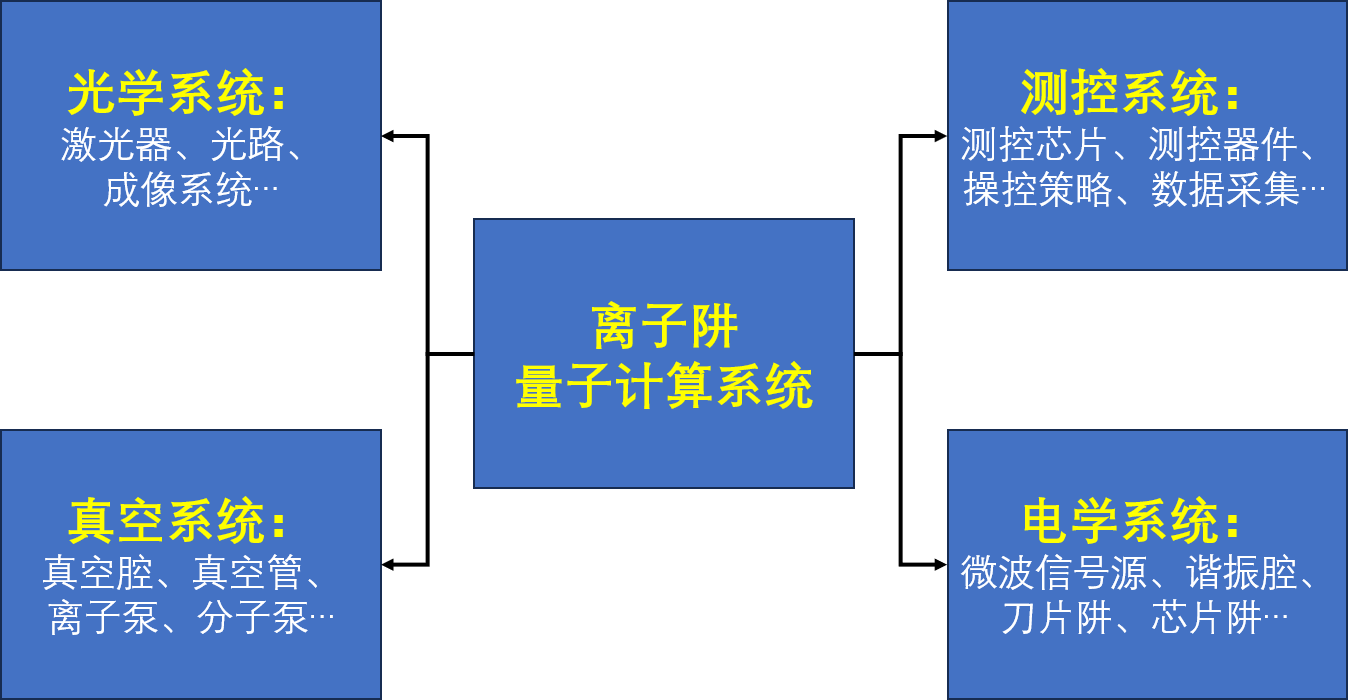
\includegraphics[width=0.8\linewidth]{quantum_computing_ion_trap_system}
% \end{figure}

离子阱量子计算系统是一个复杂综合的系统,
% 如图\ref{fig:quantum_computing_ion_trap_system}所示,
它主要由四大部分组成:1.  电学系统,主要包括微波信号源、谐振腔、阱电极等;2. 光学系统,主要包括激光器、由各类镜片组成的光路、成像系统等;3. 真空系统,主要包括真空腔、真空管、离子泵、分子泵等;4. 测控系统,主要包括测控芯片、测控器件以及配套的硬件和软固件等。想要实现基于离子阱的量子计算需要以上各大部分的相互配合。
其中量子测控系统处于十分核心的地位,它将电学、光学、真空等其余各个部分联系了起来,给出特定时序的微波、激光等信号对量子比特进行调控并采集结果进行分析和处理。
量子物理实验常常涉及到一些物理量的精确调控和测量,这既包括强度上的精确性,也包括时间上的精确性。随着量子技术的发展,量子物理实验系统也开始产生对数据处理、复杂流程控制和实时计算的需求。
% 不同于传统行业,量子物理实验系统对时间控制的精度和分辨率的要求在纳秒量级、延迟要求在百纳秒至数十微秒量级\cite[]{Ryan_Johnson_Ristè_Donovan_Ohki_2017,Guo_Qin_Schulz_2023},与当前微处理器的主频相当,这对量子物理实现的测控系统提出了很多新的要求。
具有更强实时性、更好可拓展性、集成度更高的量子测控系统对量子计算领域的发展至关重要。

% \subsection[量子测控]{量子测控}
现有的实时系统一般使用主频在数百MHz至GHz量级的通用微处理器或微控制器作为控制的主体,以计时器中断和时间片分配等方式实现实时控制。这一方案成立的前提是时间控制精度与指令执行频率之间有3-6个数量级的差异,可忽略处理器架构和中断系统的不确定性。
% 然而近来随着量子技术的发展,量子物理实验系统也开始产生对数据处理、复杂流程控制和实时控制的需求。
不同于传统行业,量子物理实验系统对时间控制的精度和分辨率的要求在纳秒量级、延迟要求在百纳秒至数十微秒量级\cite[]{Ryan_Johnson_Ristè_Donovan_Ohki_2017,Guo_Qin_Schulz_2023,junhua03},与当前微处理器的主频相当,从而前述的现有的实时控制方案难以满足需求。
因此早年在量子物理实验领域内,通常用FPGA(现场可编程门阵列)设计特定的时序脉冲发生器来产生高时间精度的脉冲序列,以此作为其它实验设备的触发信号,进行准确的时序控制。然而,这类方案的灵活性较差,只能产生预定的序列,无法在实验中对实验数据进行即时的处理,或根据实验的中间结果对后续的流程进行及时的调整\cite[]{junhua01}。随着量子算法发展,实验方案复杂,需在数十纳秒至数十微秒内处理中间结果并确定后续流程,简单的时序脉冲发生器已无法满足,实验测控系统需具备通用计算能力。

当前解决问题的思路是另置通用微处理器处理实验数据和产生时序。对于离子阱量子计算体系,量子物理高级实时基础设施(ARTIQ)\cite[]{Bourdeauducq_Jördens_Zotov_Britton_Slichter_Leibrandt_Allcock_Hankin_Kermarrec_Sionneau_et_al_2016}是控制量子物理实验的硬件、固件和软件的完整且免费开源框架。这也是目前大多数离子阱量子计算领域实验组所使用的测控系统技术方案。然而,ARTIQ的控制流架构使用在FPGA中实现的通用CPU,即所谓的软核CPU。这种方案虽然已经可以满足当前的离子阱量子实验需求,但是其进一步的拓展也受到多器件同步以及通信时延的影响而受限,并且对于对事件响应速率要求更高的超导量子比特实验难以保证可用性。针对超导量子计算的需求,来自UCSB/Google\cite[]{Chen_Sank_O’Malley_White_Barends_Chiaro_Kelly_Lucero_Mariantoni_Megrant_et_al_2012, Sank_Jeffrey_Mutus_White_Kelly_Barends_Chen_Chen_Chiaro_Dunsworth_et_al}、ETH Zurich\cite[]{Steffen_Salathe_Oppliger_Kurpiers_Baur_Lang_Eichler_Puebla_Hellmann_Fedorov_Wallraff_2013}、TU Delft\cite[]{Riste_Dukalski_Watson_Lange_Tiggelman_Blanter_Lehnert_Schouten_DiCarlo,Bultink_Rol_OBrien_Fu_Dikken_Dickel_Vermeulen_de_Sterke_Bruno_Schouten_et_al_2016}和Yale\cite[]{Ofek_Petrenko_Heeres_Reinhold_Leghtas_Vlastakis_Liu_Frunzio_Girvin_Jiang_et_al_2016}的研究者们也使用FPGA开发了自己的量子测控系统,且在进行将其应用到低温系统中的探索\cite[]{Homulle_Visser_Patra_Ferrari_Prati_Sebastiano_Charbon_2017, Conway_Lamb_Colless_Hornibrook_Pauka_Waddy_Frechtling_Reilly_2016},但是他们的这些软件都是不向整个量子计算社区开放的。
近几年来,随着量子计算领域的蓬勃发展,很多商业公司也逐步参与到量子测控系统的研发之中。Colm A. Ryan等人\cite[]{Ryan_Johnson_Ristè_Donovan_Ohki_2017}描述了雷声BBN技术公司为超导量子比特的动态量子信息处理实验开发的硬件、网关和软件。该方案的读出和控制平台都广泛地使用FPGA,使得量子比特控制系统的重构和迭代更加方便。但是该方案依赖两个独立器件(量子数字信号发生器(QDSP)和 任意波形发生器APS)的配合完成比特的读出和控制,其进一步的规模化拓展仍然受限于设备间的通信速率及设备的运算能力。

总体来说,这种面向量子领域的测控系统很难依靠经典CPU实现,当前大多数研究者开发的系统都是基于经典CPU+FPGA或者在FPGA上实现经典软核CPU的方式实现的,大都存在微处理器和时序脉冲发生器相互独立、同步困难的问题,会复杂化时序设计并产生时间浪费,影响其性能的进一步提升。
这些方案的另一问题在于,当系统规模较大,一个时序脉冲发生器无法控制整个系统时,就需要同时使用多个时序脉冲发生器,而一个微处理器同时处理过多的实验数据、同时控制过多的时序脉冲发生器,将不可避免的产生拥塞,这会进一步加剧前述的同步性问题。而如果同时使用多个微处理器,则不同微处理器之间的同步性又将成为问题。此外,当前主流的微处理器架构和指令集都是针对通用计算而优化的,主流的微处理器使用的通信协议都是针对高吞吐率而优化的,二者都难以实现精确的时序同步。
% 因此,一种能满足量子实时控制和信息处理的可大规模拓展的测控系统需求迫切,这种量子测控系统的实现可能需要专门设计强实时的微处理器架构以及相应的指令集,并且对于其大规模拓展也应具备强大的系统间同步能力。


尽管到目前为止离子阱量子计算发展迅速,但在实现通用量子计算机之前仍有许多问题有待解决。其中十分重要的一方面是量子测控系统\cite[]{Bourdeauducq_Jördens_Zotov_Britton_Slichter_Leibrandt_Allcock_Hankin_Kermarrec_Sionneau_et_al_2016,Chen_Sank_O’Malley_White_Barends_Chiaro_Kelly_Lucero_Mariantoni_Megrant_et_al_2012,Sank_Jeffrey_Mutus_White_Kelly_Barends_Chen_Chen_Chiaro_Dunsworth_et_al,Steffen_Salathe_Oppliger_Kurpiers_Baur_Lang_Eichler_Puebla_Hellmann_Fedorov_Wallraff_2013},一种能满足量子实时控制和信息处理的可大规模拓展的测控系统需求迫切,这种量子测控系统的实现可能需要专门设计强实时的微处理器架构以及相应的指令集,并且对于其大规模拓展也应具备强大的系统间同步能力。
除此之外,许多研究者也致力于芯片离子阱\cite[]{Mehta_Eltony_Bruzewicz_Chuang_Ram_Sage_Chiaverini_2014}、离子穿梭和规模化\cite[]{Monroe_Kim_2013, Sterling_Rattanasonti_Weidt_Lake_Srinivasan_Webster_Kraft_Hensinger_2014, Lee_Jeong_Park_Jung_Kim_Cho_2021}、光学集成\cite[]{Niffenegger_Stuart_Sorace_Agaskar_Kharas_Bramhavar_Bruzewicz_Loh_Maxson_McConnell_Reens_et_al_2020, Mehta_Zhang_Malinowski_Nguyen_Stadler_Home_2020}、多离子的单独寻址\cite[]{Ivory_Setzer_Karl_McGuinness_DeRose_Blain_Stick_Gehl_Parazzoli_2020}和量子比特纠错\cite[]{Cramer_Kalb_Rol_Hensen_Blok_Markham_Twitchen_Hanson_Taminiau_2016,Reichardt_2021}等技术,以实现最终目标——\emph{通用量子计算机(Universal Quantum Computer, UQC)}。

\section[论文章节结构介绍]{论文章节结构介绍}
% \textcolor{red}{简要阐述一下后续章节的主要内容...}
离子量子计算是当前最具发展前景的量子计算平台之一,它的实现需要电子学、光学、真空、测控等多种学科领域的支持。其中测控系统扮演着十分重要的角色,
% 测控系统涵盖着十分广阔的范围,包括测控核心板卡以及由其构成的如结合螺线管谐振腔的离子阱频率稳定、结合激光器的激光功率和激光拍频稳定等相关测控子系统。
以面向离子阱量子计算的实验测控系统研究为主旨,本文后续的章节结构如下:
\begin{itemize}
    \item 第\ref{section:quantum_computation}章,介绍囚禁离子量子比特的相关内容,以分析和明确量子物理实验对测控系统的切实需求。内容包括离子囚禁和量子化过程中涉及的在囚禁势场中的经典和量子运动,离子运动的量子化和离子与光场的耦合,离子(具体来说是镱离子)作为量子比特的编码和操控方案以及基于离子的通用量子门的构建;
    \item 第\ref{section:fpga_rtmq}章,引入了一种强实时性、可拓展性好、高度数字化和集成化的测控系统架构——RTMQ,以满足量子物理实验对测控系统的更高要求。同时也对RTMQ微处理器所配套设计的汇编指令集和多节点同步的实时通信链路系统进行了描述和分析,为后续量子测控板硬件设计及其功能拓展的实现和应用打下基础;
    \item 第\ref{section:helical}章,针对螺线管谐振腔这种离子囚禁系统中的重要射频器件进行了仿真、实验、建模、设计等方面的优化研究。谐振腔更高的Q值可以提高离子囚禁的稳定性和离子比特的保真度,针对螺线管谐振腔的Q值和频率运用有限元仿真软件HFSS进行了仿真模型的建立并与实验制作测量结果进行了验证。同时,针对旧有谐振腔惯用机械结构设计的缺点,给出了一种更加稳定易用、更模块化且装配方便的谐振腔机械结构设计;
    \item 第\ref{section:implementation}章,基于RTMQ测控系统架构(第\ref{section:fpga_rtmq}章),设计了一套适配的测控板硬件并实现了相应的功能外设。
    在此基础上,
    % 基于螺线管谐振腔(第\ref{section:helical}章)、激光器等器件并结合
    针对实验系统对量子比特操作保真度的实际需求,实现了RTMQ测控系统在离子量子计算应用场景下的几个关键子系统搭建和测试,包括离子阱频率稳定、激光功率稳定和激光拍频稳定等,展示了RTMQ系统的优越性。
    在此过程中也给出了高速通用数字PID和高速通用数字IIR滤波器的设计及FPGA实现。基于RTMQ架构的测控板的使用极大地促进了离子量子计算系统的数字化、集成化进程,同时也可以满足未来大规模通用量子计算对可拓展性的需求;
    \item 最后一章,对本论文进行了总结。
    % 并对离子量子计算及量子测控领域未来的发展进行了展望。
\end{itemize}
% !TeX root = ../sustechthesis-example.tex

\chapter[囚禁离子量子比特]{囚禁离子量子比特\label{section:quantum_computation}}
% \textcolor{red}{
% 介绍离子在离子阱中的经典和量子运动、介绍离子的一些特别的运动量子态;
% 讲一下离子量子比特的主要特点(一致性、全连接性、相干时间长等)、介绍一下单比特门操作的主要方案(微波、激光拉曼);离子的运动不用讲太多,先讲囚禁,再讲一下运动的量子化、拉曼光对运动的耦合以及M-S门就行,特殊量子态可以不用讲,或至少不用大篇幅。这里M-S门部分可以给后面Helical部分做点铺垫,讲一下阱频率对门操作保真度和操作时间的影响。
% 整体而言,离子量子比特的量子态制备、探测和单比特门一个小节,运动部分再2个小节,差不多。
% }
量子测控是量子计算系统中的重要组成部分,相对于传统测控系统来说,量子测控系统的特别之处在于它不仅需要具备经典场景下的信息处理能力,还需要具备量子场景下的信息处理能力。总体来说,量子物理场景对测控系统提出了实时性、拓展性、信息处理方式等方面的新需求。对于离子量子计算来说,具体需求的认识和处理都需要我们对目标系统拥有充分的了解,这样才能更好地开发、优化和部署适宜的测控系统。
本章内容将介绍与量子测控系统紧密相关的离子量子计算的重要背景以分析和理解其切实需求,内容包括离子的囚禁及其涉及到的经典和量子运动,特别地,针对当前实验室所使用的镱离子介绍它的能级结构、比特编码、比特控制,以及基于离子构建的通用量子门。


\section[离子的囚禁及在阱中的经典和量子运动]{离子的囚禁及在阱中的经典和量子运动\label{section:ion_trap_motion}}
离子阱量子计算的一个最基本的问题就是获得在空间中稳定存在的离子,利用其具备的量子特性来作为量子计算的比特载体。离子阱采用射频阱对离子进行动态囚禁,最具代表性的一类是四极阱,它及它的一些变型也是目前在离子阱量子计算研究中应用最广泛的一类离子阱。四极阱的电势描述如下:
\begin{align}
    % \label{eq:quadrupolar_trap_potential}
    \Phi(x, y, z, t) = &U\frac{1}{2}(\alpha x^2 + \beta y^2 + \gamma z^2) \label{eq:time_independent_part}\\
    \label{eq:time_dependent_part}
    &+ \tilde{U}\cos (\omega_{rf}t)\frac{1}{2}(\alpha ' x^2 + \beta ' y^2 + \gamma ' z^2) 
\end{align}

其中$\Phi(x, y, z, t)$是四极阱的电势,$U$和$\tilde{U}$分别是静态和动态信号的幅值,$\omega_{rf}$是动态信号的频率,$\alpha, \beta, \gamma$及$\alpha', \beta', \gamma'$。公式\eqref{eq:time_independent_part}是不依赖时间的项,公式\eqref{eq:time_dependent_part}是随时间变化的项。整个电势的表达式每时每刻都要满足拉普拉斯方程(Laplace equation)$\Delta \Phi=0$的约束条件,从中可以导出整个四极阱的几何参数约束:
\begin{align}
    \alpha + \beta + \gamma =0,\\
    \alpha ' + \beta ' + \gamma ' =0
\end{align}

其中各参数的定义在公式\eqref{eq:time_independent_part}和公式\eqref{eq:time_dependent_part}定义。从这些限制可以明显看出,在自由空间中电势不可能稳定地产生局部三维最小值,因此电势只可能以动态方式来对离子进行囚禁。通过选择合适的四极阱几何参数,再结合适当的驱动微波的频率和驱动电压我们可以做到这一点,其中一种几何参数选择如下:
\begin{align}
    -(\alpha + \beta )= \gamma > 0,\\
    \alpha ' = - \beta '
\end{align}

这种几何参数的设置会使离子在$x,y$平面上动态地被囚禁,在$z$方向上静态地被囚禁。在这种设置的离子阱中,多个离子会沿着$z$轴形成线性的离子链,这便是人们所知的\emph{线性离子阱(Linear Trap)},也被称为\emph{Paul Trap}\cite[]{Paul_1990}。


\subsection[离子在RF阱中的经典运动]{离子在RF阱中的经典运动\label{section:ion_classical_motion}}

在接下来的两小节里将介绍囚禁离子的经典运动方程及其解析解(第\ref{section:classical_motion}节),并给出这些解的低阶近似(第\ref{section:lowest_order_approximation}节)。

\subsubsection[经典运动方程]{经典运动方程\label{section:classical_motion}}

一个质量为$m$电荷量为$Z|e|$的粒子在如公式\eqref{eq:time_independent_part}所描述的电场中的经典运动方程由Paul等人\cite[p415]{Paul1958}给出。粒子的运动在空间坐标方向上中是解耦的。下面只讨论$x$方向上的运动;其他方向可以类似地处理。运动方程如下:
\begin{align}
    \ddot{x}=-\frac{Z|e|}{m}\frac{\partial \Phi}{\partial x}=-\frac{Z|e|}{m}[U\alpha + \tilde{U}\cos(\omega_{rf}t)\alpha ']x
\end{align}

经过下面的参数代换,这个方程可以转化为标准的\emph{马修方程(Mathieu Equation, ME)}形式:
\begin{align}
    \frac{d^2x}{d\xi^2}+[a_x-2q_x\cos(2\xi)]x=0\label{eq:mathieu_equation}
\end{align}

相应的参数代换为:
\begin{align}
    \xi=\frac{\omega_{rf}t}{2},\ a_x=\frac{4Z|e|U\alpha}{m\omega_{rf}^2},\ q_x=\frac{2Z|e|\tilde{U}\alpha '}{m\omega_{rf}^2}\label{eq:parameters_substitution}
\end{align}

ME方程属于一般的周期系数微分方程。它的稳定解的一般形式可以由\emph{弗洛奎定理(Floquet Theorem)}导出\cite[]{McLachlan, McQuarrie}:
\begin{align}
    x(\xi)=&Ae^{i\beta_x\xi}\sum_{n=-\infty}^{\infty}C_{2n}e^{i2n\xi}\\
    &+ Be^{-i\beta_x\xi}\sum_{n=-\infty}^{\infty}C_{2n}e^{-i2n\xi}\label{eq:mathieu_solution}
\end{align}

其中实值特征指数$\beta_x$和系数$C_{2n}$仅是$a_x$和$q_x$的函数,不依赖于初始条件。$A$和$B$是任意常数,可用于满足边界条件或规格化特解。将公式\eqref{eq:mathieu_solution}代入公式\eqref{eq:mathieu_equation}可以得到一个递归关系:
\begin{align}
    C_{2n+2}-D_{2n}C_{2n}+C_{2n-2}=0,\\
    D_{2n}=[a_x-(2n+\beta_x)^2]/q_x\label{eq:recursion_raltion}
\end{align}

这一递归关系将实值特征指数$\beta_x$、系数$C_{2n}$与$a_x$、$q_x$联系起来。通过进一步地整理也可以得到$C_{2n}$的表达式:
\begin{align}
    C_{2n+2}=\frac{C_{2n}}{D_{2n}-\frac{1}{D_{2n+2}-\frac{1}{\dots}}}\\
    C_{2n}=\frac{C_{2n-2}}{D_{2n}-\frac{1}{D_{2n-2}-\frac{1}{\dots}}}\label{eq:c_2n_fraction}
\end{align}

利用结合上述公式$\beta_x$也可以计算:
\begin{align}
    \beta_x^2=a_x-q_x\left(\frac{1}{D_0-\frac{1}{D_2-\frac{1}{\dots}}} + \frac{1}{D_0-\frac{1}{D_{-2}-\frac{1}{\dots}}}\right) \label{eq:beta_x_fraction}
\end{align}

可以根据所需的精度,选择截断公式\eqref{eq:c_2n_fraction}和公式\eqref{eq:beta_x_fraction}中的连分式来获取相应的结果。
实际上,对于实验中常用到的典型$a_x$和$q_x$值,连分式中高阶项的贡献会迅速下降。

% \textcolor{red}{这里的$a_x, q_x$具体的含义后面有时间了可以再看看。}

\subsubsection[低阶近似]{低阶近似\label{section:lowest_order_approximation}}
实际实验系统中采用的在公式\eqref{eq:parameters_substitution}中定义的参数往往是满足$(|a_x|,q_x^2)\ll 1$的。在此条件下,假设$C_{\pm 4}\simeq 0$,则可以得到$x(t)$轨迹的\emph{低阶近似(Lowest-order Approximation)}。再同时设置初始条件$A=B$,公式\ref{eq:recursion_raltion}可以得到:
\begin{align}
    \beta_x\approx \sqrt{a_x+q_x^2/2},\\
    x(t)\approx2AC_0\cos\left(\beta_x\frac{\omega_{rf}}{2}t\right)\left[1-\frac{q_x}{2}\cos(\omega_{rf}t)\right]\label{eq:classical_motion_solution}
\end{align}

囚禁离子在$x$方向上的轨迹$x(t)$的由频率为$\nu=\beta_x\omega_{rf}/2\ll \omega_{rf}$的谐波振荡叠加频率为$\omega_{rf}$的RF频率造成的\emph{驱动位移}组成,分别称为\emph{长期运动(Secular-motion)}和\emph{微运动(Micro-motion)}两者相位相差$180^\circ$;
离子在离子阱中的微运动的频率为$\omega_{rf}\ll \nu$,且其振幅为长期运动振幅的$q_x/2\ll 1$,这也是它被称为微运动的原因。如果忽略微运动,则长期运动可以近似为频率为$\nu$的谐振子的运动。在大多数情况下,如果离子处于相当低的动能,即使我们用量子力学的方法来处理离子的质心运动,这个处理也是合理的。


\subsection[离子在RF阱中的量子力学运动]{离子在RF阱中的量子力学运动\label{section:quantum_motion}}
% \textcolor{red}{主要参考文献\cite[chap2-B]{Leibfried_Blatt_Monroe_Wineland_2003}}

如第\ref{section:ion_classical_motion}节中已经讨论过的,经典中的运动分析似乎已经可以很好地描述离子在离子阱中的运动了。但是,由于四极阱产生的囚禁势场不是静态的而是与时间相关的,因此不能理所当然地认为在有效时间平均势中量化运动已经为我们提供了囚禁离子足够的图景。实际上,在离子阱的实验中,即使是对离子阱中的冷却过程的简单解释,以及对非经典状态的描述,也都依赖于运动的量子力学图景的。

在接下来的两小节里,我将根据文献\cite[]{Arimondo_Phillips_Strumia_1992}中的方法导出囚禁离子在射频场中的量子力学表述。同时在这里讨论,在实验中使用的捕获参数范围内,囚禁离子的量子化运动可以用静态谐振子来近似。

\subsubsection[量子力学运动方程]{量子力学运动方程}
对于囚禁离子运动的量子力学处理,我们假设与时间相关的势在囚禁离子质心的三个笛卡尔坐标中的每一个中都是二次的(一维谐振子势\cite[]{Solimeno_Di_Porto_Crosignani})。然后,与经典运动一样,问题可分为三个一维问题。在一维中,用各自的算子$\hat{x}$替换坐标$x$,于是可以将与时间相关的势$V(T)$写为:
\begin{align}
    V(t)=\frac{m}{2}W(t)\hat{x}^2
\end{align}

其中,
\begin{align}
    W(t)=\frac{\omega_{rf}^2}{4}\left[a_x+2q_x\cos(\omega_{rf}t)\right]
\end{align}

可以被认为是一个时变弹簧常数,它的作用类似于在静态势谐振子中$\omega^2$的作用。在以上的定义下,囚禁离子运动的哈密顿量$H^{(m)}$的形式和我们在量子力学中处理的静态谐振子的哈密顿量很相似:
\begin{align}
    \hat{H}^{(m)}=\frac{\hat{p}^2}{2m}+\frac{m}{2}W(t)\hat{x}^2\label{eq:static_harmiltonian_oscillator}
\end{align}

于是我们可以很轻松地写出这些运动算子在\emph{海森堡图景(Heisenberg Picture)}下的的方程:
\begin{align}
    \dot{\hat{x}}= \frac{1}{i\hbar}\left[\hat{x,\hat{H}^{(m)}}=\frac{\hat{p}}{m}\right],\\
    \dot{\hat{p}}= \frac{1}{i\hbar}\left[\hat{p},\hat{H}^{(m)}\right]=-mW(t)\hat{x}
\end{align}

他们的一个更紧凑的方程形式如下:
\begin{align}
    \ddot{\hat{x}}+W(t)\hat{x}=0 \label{eq:quantum_motion_equation}
\end{align}

如果用函数$u(t)$替换算子$\hat{x}$,我们可以很容易验证这个公式\eqref{eq:quantum_motion_equation}与\emph{马修方程}\eqref{eq:mathieu_equation}是等价的。这就是我们能够借助前面所叙述的马修方程的解来寻找公式\eqref{eq:quantum_motion_equation}的解。添加边界条件:
\begin{align}
    u(0)=1,\ \hat{u}(0)=i\nu \label{eq:boundary_condition}
\end{align}

这对应于公式\eqref{eq:mathieu_solution}中的$A=1,\ B=0$,可以得到:
\begin{align}
    u(t)=e^{i\beta_x\omega_{rf}/2}\sum_{n=-\infty}^{\infty} C_{2n}e^{i n\omega_{rf}t}\equiv e^{i\beta_x\omega_{rf}t/2}\Phi(t) \label{eq:ut_expression}
\end{align}

其中$\Phi(t)$是一个周期为$T=2\pi/\omega_{rf}$的周期函数。于是公式\eqref{eq:boundary_condition}变为:
\begin{align}
    u(0)=\sum_{n=-\infty}^{\infty}C_{2n}=1,\ \nu = \omega_{rf}\sum_{n=-\infty}^{\infty}C_{2n}(\beta_x/2+n)
\end{align}

这个解及其复共轭是线性独立的;因此,它们服从\emph{Wronskian恒等式}:
\begin{align}
    u^*(t)\dot{u}(t)-u(t)\dot{u}^*(t)=u^*(0)\dot{u}(0)-u(0)\dot{u}^*(0)=2 i \mu
\end{align}

未知坐标$\hat{x}(t)$和$u(t)$满足相同的微分方程,因此复杂的线性组合:
\begin{align}
    \hat{C}(t)=\sqrt{\frac{m}{2\hbar \nu}}i\left\{u(t)\dot{\hat{x}(t)-\dot{u}(t)\hat{x}(t)}\right\} \label{eq:complex_combination}
\end{align}

与其如下的Wronskian恒等式成正比,并且在时间上也是恒定的:
\begin{align}
    \hat{C}(t)=\hat{C}(0)=\frac{1}{\sqrt{2m \hbar \nu}}\left[m\nu\hat{x}(0)+i\hat{p}(0)\right]
\end{align}

此外,等式右边恰好是质量$m$和频率$\nu$的在静态谐振子势场中的湮灭算符:
\begin{align}
    \hat{C}(t)=\hat{C}(0)=\hat{a}
\end{align}

也就是说有如下式:
\begin{align}
    \left[\hat{C},\hat{C}^\dagger\right]=\left[\hat{a},\hat{a}^\dagger\right]=1
\end{align}

这个静态势场中的谐振子在后续将被称为\emph{参考谐振子(Reference Oscillator)}。

海森堡算符$\hat{x}(t)$和$\hat{x}(t)$可以用$u(T)$和参考振荡器的算符用公式\eqref{eq:complex_combination}重新表示:
\begin{align}
    \hat{x}(t)=\sqrt{\frac{\hbar}{2m\nu}}\left\{\hat{a}u^*(t)+\hat{a}^\dagger u(t)\right\},\\
    \hat{p}(t)=\sqrt{\frac{\hbar m}{2\nu}}\left\{\hat{a}\dot{u}^*(t)+\hat{a}^\dagger \dot{u}(t)\right\}
\end{align}

所以囚禁离子的整个时间依赖性由特殊解$u(t)$及其复共轭给出。
这样一来,对于接下来的计算,在海森堡图景中表述一些列的时间依赖波函数就很方便了。同样,上面使用的参考振荡子也将非常有帮助。与静态势的情况类似,我们将考虑一系列的基态$\ket{n,t}$,其中$n=1,2,\dots,\infty$。这些状态被称为谐波振荡器\emph{数态(Fock States)}的动态对应物。参考振荡子$\ket{n=0}_\nu$的基态满足条件:
\begin{align}
    \hat{a}\ket{n=0}_\nu=\hat{C}(t)\ket{n=0}_\nu=0 \label{eq:obey_condition}
\end{align}

由于海森堡算子$\hat{C}$是通过$\hat{C}(t)=\hat{U}^\dagger(t)\hat{C}_S\hat{U}(t)$与$\hat{C}_S$联系起来的,我们可以很快得到(其中$\hat{U}(t)=\exp{\left[-(i/\hbar)\hat{H}^{(m)}\right]}$):
\begin{align}
    \hat{C}_S(t)\hat{U}(t)\ket{n=0}_\nu=\hat{C}_S(t)\ket{n=0,t}=0 \label{eq:oscillator_condition}
\end{align}

只需要通过将公式\eqref{eq:obey_condition}左侧与$\hat{U}(t)$相乘,并注意到$\hat{U}(t)\ket{n=0}_\nu$是从静态潜在参考振荡子的基态演变而来的时间相关振荡器的薛定谔态。由于薛定谔算子$C_S(t)$的时间依赖完全取决于$u(t)$的时间演化,于是公式\eqref{eq:oscillator_condition}等价于:
\begin{align}
    \left[u(t)\hat{p}-m\dot{u}\hat{x}\right]\ket{n=0,t}=0
\end{align}

在坐标空间表述为:
\begin{align}
    \left\{u(t)\frac{\hbar}{i}\frac{\partial}{\partial x'}\right\}\braket{x'|n=0,t}=0
\end{align}

归一化后的解为:
\begin{align}
    \braket{x'|n=0,t}=\left(\frac{mv}{\pi\hbar}\right)^{1/4}\frac{1}{\{u(t)\}^{1/2}}\exp\left[\frac{i m}{2\hbar}\frac{\dot{u}(t)}{u(t)}x'^2\right]
\end{align}

与静态势谐振子完全类似,可以通过创建算子$\hat{C}_S^\dagger(t)$对基态重复操作来创建完全正交基的所有其它状态:
\begin{align}
    \ket{n,t}=\frac{\left[\hat{C_S^\dagger(t)}\right]^n}{\sqrt{n!}}\ket{n=0,t}\label{eq:basic_sattes}
\end{align}

将$u(t)$如公式\eqref{eq:ut_expression}重写后,在坐标空间表述为:
\begin{align}
    \braket{x'|n,t}=\exp\left[-i\left(n+\frac{1}{2}\right)\nu t\right]\chi_n(t) \label{eq:quantum_states_expression}
\end{align}

其中,$H_n$是$n$阶厄米多项式,$\chi_n(t)$表达式如下:
\begin{align}
    \chi_n(t)=\frac{1}{\sqrt{2^n n!}}\left(\frac{m\nu}{\pi  \hbar}\right)^{1/4}
    \frac{\exp\{-i n \arg\left[\Phi(t)\right]\}}{\{\Phi(t)\}^{1/2}}\\
    \times H_n\left\{\left[\frac{m\nu}{\hbar|\Phi|^2}\right]^{1/2}x'\right\}\\
    \times \exp\left\{\frac{m\nu }{2\hbar}\left[1-\frac{i\Phi(t)}{\nu\Phi(t)}\right]x'^2\right\}
\end{align}

经典的微运动作为射频驱动场周期的脉动出现在波函数中。对于静态势谐振子,能量本征态的演化只将波函数乘以相位因子(这就是为什么它们被称为静止态)。在此处研究的时间相关电势场中,同样如此,不同之处仅在于这里时间只能取得RF周期$T=2\pi/\omega_{rf}$的整数倍。公式\ref{eq:quantum_states_expression}给出的状态并不是能量本征态(它们周期性地与驱动场交换能量,类似于经典的微运动),但它们是时间相关势中可能的平稳状态的很好的近似。因此,它们通常被称为\emph{准平稳状态(Quasistationary States)}。

紧接着的小结节中将介绍与第\ref{section:lowest_order_approximation}节中提出的经典伪势解类似的量子力学中的运动解的低阶近似,找到对静态势谐振子图景的最低阶修正。


\subsubsection[量子低阶近似]{量子低阶近似}
量子力学中的低阶近似从导出$u(t)$的近似表达开始。与经典的情况类似,低阶近似需要满足条件:$|a_x|,q_x^2\ll 1$、$C_{\pm 4}=0$。结合公式\eqref{eq:boundary_condition}中的初始条件可以得到:
\begin{align}
    \beta_x\approx\sqrt{a_x+q_x^2/2},\ \nu\approx\beta_x\omega_{rf}/2,\\
    u(t)\approx\exp{i\nu t}\frac{1+(q_x/2)\cos(\omega_{rf}t)}{1+q_x/2}\label{eq:quantum_lowest_order_approximation}
\end{align}

这实质上就是前面第\ref{section:lowest_order_approximation}节在公式\eqref{eq:classical_motion_solution}中找到的经典解。
仍然必须强调的是,只有在这种低阶近似中,参考谐振子的频率$\nu$才等于特征指数$\beta_x\omega_{rf}/2$。现在很明显地可以看出$\chi_n(t)$以周期$T_{rf}$进行周期性呼吸。具体可以从基态波函数的近似表达式$\chi_0(t)$中看到:
\begin{align}
    \chi_0(t)=\left(\frac{m\nu}{\pi \hbar}\right)^{1/4}\sqrt{\frac{1+q_x/2}{1+(q_x/2)\cos(\omega_{rf}t)}}
    \times \exp\left(\left\{i\frac{m\omega_{rf}\sin(\omega_{rf}t)}{2\hbar\left[1/q_x+\cos(\omega_{rf}t)\right]}-\frac{m\nu}{2\hbar}\right\}x'^2\right)
\end{align}

而公式\eqref{eq:quantum_states_expression}中的相位因子由基态伪能量$\hbar\nu/2$控制。如果设置$\omega_{rf}=0$,则这个表达式与静态谐波势基态波函数相同。



\subsection[囚禁离子的光场耦合]{囚禁离子的光场耦合}
% \textcolor{red}{这部分主要参考文献\cite[p3-8]{Leibfried_Blatt_Monroe_Wineland_2003}}

想要用离子实现量子计算,需要用一定的方式作用于离子对其进行操控。通过对离子施加合适的电磁场,可以使得囚禁离子的内部能级相互相干耦合,并且也可以与离子的外部运动自由度耦合。
囚禁良好和耦合度高的离子可以被看作为
\emph{Jaynes-Cummings 哈密顿量(Jaynes-Cummings Hamiltonian)}\cite[]{Janszky_Yushin_1986}
因此,许多致力于囚禁离子相干相互作用的工作都受到这种耦合在量子光学中所起的重要作用的启发。
除了上面这种特殊情况之外,其余多种可能得情况下会涉及到多个运动量子之间的相互交换,类似于量子光学中的多光子跃迁。
此外,原子-光子耦合中隐含的能量守恒不必局限在囚禁离子的内部态和运动态之间的转换,也可以实现囚禁离子内部态的相互转换,比如吸收来自耦合光场的能量跃迁到更高的能级上。
最后,如果考虑了运动方面的全量子力学图景,包括微运动引起的修正,则另一类跃迁可能需要被考虑,涉及到在离子阱的RF电势中运动态整数倍数的相互转换或驱动场整数倍数的组合和长期运动(微运动边带)。

% \subsection[囚禁离子的光场耦合]{囚禁离子的光场耦合}
\subsubsection[二能级近似]{二能级近似\label{section:two_level_approximation}}
在常规的离子阱研究中,会把囚禁离子的电子能级结构近似为\emph{二能级系统(Two-level System)},这为研究提供了很大的方便。这个二能级系统表示为$\ket{g}$和$\ket{e}$,他们之间有着$\hbar \omega=\hbar(\omega_e-\omega_g)$的能量差。这对于实际的囚禁离子不总是适用的,仅在广场与离子两能级近似共振耦合且耦合的拉比频率远强于衰减到其它态的强度时才成立。不过这个条件对当今研究的多数实验系统中的离子(如镱离子、钡离子、钙离子等等)来说都是成立的。
相应的二能级哈密顿量$\hat{H}^{(e)}$的表述如下:
\begin{align}
    \hat{H}^{(e)}=\hbar(\omega_g\ket{g}\bra{g}+\omega_e\ket{e}\bra{e})\\
    =\hbar\frac{\omega_e+\omega_g}{2}(\ket{g}\bra{g}+\ket{e}\bra{e})\\
    +\hbar\frac{\omega}{2}(\ket{g}\bra{g}-\ket{e}\bra{e}) \label{eq:two_level_hamiltonian}
\end{align}

任何二能级系统有关的算子都可以被映射到$1/2$自旋算子基矢上,因此上述的$\hat{H}^{(e)}$及其相关的算子也可以被表示为泡利矩阵的形式,它们之间的映射关系如下:
\begin{align}
    \ket{g}\bra{g}+\ket{e}\bra{e}\mapsto \hat{I},\ \ket{g}\bra{e}+\ket{e}\bra{g}\mapsto \hat{\sigma}_x,\ \\
    i(\ket{g}\bra{e}-\ket{e}\bra{g})\mapsto \hat{\sigma}_y,\ \ket{e}\bra{e}-\ket{g}\bra{g}\mapsto \hat{\sigma}_z
\end{align}

在这种映射情况下,$\hat{H}^{(e)}$可以被表述为:
\begin{align}
    \hat{H}^{(e)}=\hbar\frac{\omega}{2}\sigma_z
\end{align}

相应的能量以$-\hbar(\omega_e+\omega_g)/2$重新缩放,以抑制公式\eqref{eq:two_level_hamiltonian}中与状态无关的能量贡献。

\subsubsection[耦合的理论表述]{耦合的理论表述\label{section:coupling_theory}}

为了以一种简单而充分的方式描述囚禁离子与光场的相互作用,如前一节所述,我们假设囚禁离子的运动在所有三个维度上都是谐波的。
下面的描述将包括囚禁电势的显式时间依赖,但在许多情况下,将离子的运动建模为三维静态势谐振子是足够的。
因为如果无量纲Paul阱参数$a_x$和$q_x^2$的模量相对于与静态势和射频势(见第\ref{section:ion_classical_motion}节)远小于1,则一般理论只会引入非常微小的变化。这对于实验中常用的离子阱是成立的。
内部状态和运动耦合的广义描述遵循文献\cite[]{Cirac_Garay_Blatt_Parkins_Zoller_2002,1996Paul}中的方法。

另外还假定,在光场的多极展开中处理最低阶展开就足够了,在所讨论的近共振电子状态之间产生一个不退化的矩阵元。
电子波函数的扩展远小于耦合场的波长这一事实证明了这一假设是合理的。
对于偶极允许跃迁,将用偶极近似来处理场,而对于偶极禁止跃迁,只考虑场的四极分量。
对于拉曼跃迁,近共振的中间能级将绝热消除,使这些跃迁在形式上等同于其它类型的跃迁。

% \subsubsubsection[总哈密顿量和相互作用哈密顿量]{总哈密顿量和相互作用哈密顿量\label{section:total_hamiltonian}}
系统的总哈密顿量可以写作如下形式:
\begin{align}
    \hat{H}=\hat{H}^{(m)}+\hat{H}^{(e)}+\hat{H}^{(i)}
\end{align}

其中$\hat{H}^{(m)}$是沿着离子阱轴向的运动哈密顿量,如在第\ref{section:quantum_motion}节公式\eqref{eq:static_harmiltonian_oscillator}中讨论过的;
$\hat{H}^{(e)}$代表如第\ref{section:two_level_approximation}节中所述的离子的内部电子能级结构;
$\hat{H}^{(i)}$代表本部分将要讨论施加的光场与离子之间的耦合。

电偶极跃迁、电四极跃迁和激发拉曼跃迁可以在一个统一的框架中描述,该框架将某个共振拉比频率$\Omega$、有效光频率$\omega$和有效的波矢量$\mathbf{k}$与这些跃迁类型中的每一种相关联。
% 电偶极跃迁和电四级跃迁的耦合光场的频率和波矢量是相同的,但两者驱动受激拉曼跃迁的光场频率差$\omega=\omega_1-\omega_2$,波矢量差$\mathbf{k}=\mathbf{k_1}-\mathbf{k_2}$。
电偶极跃迁和电四级跃迁的耦合光场驱动受激拉曼跃迁的光场频率相差$\omega=\omega_1-\omega_2$,波矢量差$\mathbf{k}=\mathbf{k_1}-\mathbf{k_2}$,而两者的频率和波矢量是相同的。


对于行波光场,可以用以下形式的耦合哈密顿量来描述上面所有三种跃迁类型:
\begin{align}
    \hat{H}^{(i)}=(\hbar/2)\Omega(\ket{g}\bra{e}+\ket{e}\bra{g})\\
    \times\left[e^{i(k\hat{x}_S-\omega t + \phi)}+e^{-i(k\hat{x}_S-\omega t + \phi)}\right]
\end{align}

在$1/2$自旋代数中我们可以将其重新表述为:
\begin{align}
    \ket{e}\bra{g}\mapsto\hat{\sigma}_+=1/2(\hat{\sigma}_x+i\hat{\sigma}_y),\\
    \ket{g}\bra{e}\mapsto\hat{\sigma}_+=1/2(\hat{\sigma}_x-i\hat{\sigma}_y)
\end{align}

为了便于说明和理解,我们以一个维度的阐述为例。有效波矢量$\mathbf{k}$选为沿着离子阱中的$x$轴方向。转换到相互作用表象,可以得到自由哈密顿量$\hat{H}_0=\hat{H}_{(m)}+\hat{H}_{(e)}$与相互作用哈密顿量$\hat{V}=\hat{H}_{(i)}$的最简单的一个动力学图景。记$\hat{U}_0=\exp[-(i/\hbar)\hat{H}_0t]$,转换后的相互作用哈密顿量为:

\begin{align}
    \hat{H}_{int} &=\hat{U}_0^\dagger\hat{H}^{(i)}\hat{U}_0\\
    &=(\hbar/2)\omega e^{(i/\hbar)\hat{H}^{(e)}t}(\sigma_++\sigma_-)\\
    &\times e^{-(i/\hbar)\hat{H}^{(e)}t}e^{(i/\hbar)\hat{H}^{(m)}t}\left[e^{i(k\hat{x}-\omega t + \phi)}+e^{-i(k\hat{x}-\omega t + \phi)}\right]e^{-(i/\hbar)\hat{H}^{(m)}t}\\
    &=(\hbar/2)\Omega(\sigma_+e^{i\omega_0 t}+\sigma_-e^{-i\omega_0 t}) e^{(i/\hbar)\hat{H}^{(m)}t} \\
    &\left[e^{i(k\hat{x}-\omega t + \phi)}+e^{-i(k\hat{x}-\omega t + \phi)}\right]e^{-(i/\hbar)\hat{H}^{(m)}t}
\end{align}

上面公式表述中与时间相关的振动项提取出来后就是$\exp[\pm i (\omega\pm \omega_0)t]$。这两项一项振动频率为$\delta_f=\omega+\omega_0$,是快速振荡项;另一项振动为$\delta=\omega-\omega_0\ll \omega_0$,是慢速振荡项。在研究中我们一般会忽略快速振动项的贡献,也就是所谓的\emph{旋波近似(Rotating-wave Approximation)}。

引入\emph{Lamb-Dick参数(Lamb-Dick Parameter, LDP)}$\eta=kx_0$,其中$x_0=\sqrt{\hbar/(2m\nu)}$是参考振荡子基态波函数的$x$轴方向的扩展,海森堡图景下的$\hat{x}(t)$表述为:
\begin{align}
    k\hat{x}(t)=\eta\left\{\hat{a}u^*(t)+\hat{a}^\dagger u(t)\right\}
\end{align}

相互作用哈密顿量经过旋转波近似后的最终形式为:
\begin{align}
    \hat{H}_{int}(t)=(\hbar/2)\Omega\hat{\sigma}_+ \exp(i\{\phi+\eta[\hat{a}u^*(t)+\hat{a}^\dagger u(t)]-\delta t\})+H.c.
\end{align}

指数项中的时间依赖性由频率差$\delta$和$u(t)$控制。
考虑公式\eqref{eq:ut_expression}中的解形式及Lamb-Dicke 参数下的拓展有:
\begin{align}
    &\exp(i\{\phi + \eta [\hat{a}u^*(t)+\hat{a}^\dagger u(t)]-\delta t\})\\
    &=e^{i(\phi-\delta t)}\sum_{m=0}^{\infty} \frac{(i\eta)^m}{m!}\left\{\hat{a}e^{-i\beta_x\omega_{rf}t} \sum_{n=-\infty}^{\infty}C_{2n}^* \times e^{-i n\omega_{rf}t+H.c.}\right\}^m
\end{align}

很容易验证任何时刻的衰减满足下式:
\begin{align}
    (l'+l\beta_x)\omega_{rf}=\delta
\end{align}

其中$l$和$l'$为整数且$l\neq l', if l'\neq 0$,它们是哈密顿量中的两项慢速变化,贡献了含时变化的主要部分(其余部分可以忽略)。如果其中一个调制边带与静止离子的跃迁频率$\omega_0$重合,则该边带可以诱导离子内部状态跃迁。实际上,由于实验中$(|a_x|,q_x^2)\ll 1$,因此公式\eqref{eq:quantum_lowest_order_approximation}中的$\beta_x\omega_{rf}\approx\nu$且$C_o\approx(1+q_x/2)^{-1}$。于是相互作用哈密顿量就可以简化成如下形式:
\begin{align}
    \hat{H}_{int}(t)=(\hbar/2)\Omega_0\sigma_+ \exp\{i\eta(\hat{a}e^{-i\nu t}+\hat{a}^\dagger e^{i\nu t})\}e^{i(\phi-\delta t)}+ H.c. \label{eq:interaction_hamiltonian}
\end{align}

其中缩放的相互作用强度为$\Omega_0=\Omega/(1+q_x/2)$,这个缩放反映了射频驱动频率下波包振荡引起的耦合减少。

% \textcolor{red}{这里的波包 ‘breathing’ 应该怎么翻译?}

% \subsubsubsection[拉比频率]{拉比频率\label{section:rabi_frequency}}

依赖失谐变量$\delta$,公式\eqref{eq:interaction_hamiltonian}中的哈密顿量会耦合一定的内态和运动态。如果公式\eqref{eq:interaction_hamiltonian}在$\eta$范围内,这会产生一个包含$\sigma_{\pm}$的组合项,它有$l$个$\hat{a}$算符和$m$个$\hat{a}^\dagger$算符并以频率$(l-m)\nu=s\nu$转动。
当$\delta\approx s\nu$时,这些组合将是共振的,同时会将多态$\ket{g}\ket{n}$和$\ket{e}\ket{n+s}$耦合起来。
% 对于$s>0(s<0)$的情况,耦合强度通常称为$|s|$级\emph{蓝(红)边带}拉比频率,
对于$s>0$的情况,耦合强度通常称为$|s|$级\emph{蓝边带}拉比频率,
对于$s<0$的情况,耦合强度通常称为$|s|$级\emph{红边带}拉比频率,
表达式为\cite[]{Leibfried_Meekhof_King_Monroe_Itano_Wineland_2002, Beige_Bose_Braun_Huelga_Knight_Plenio_Vedral_2000}:
\begin{align}
    \Omega_{n,n+s}=\Omega_{n+s,n}=\Omega_0|\braket{n+s|e^{i\eta(a+a^\dagger)}|n}|\\
    =\Omega_0 e^{-\eta^2/2}\eta^{|s|}\sqrt{\frac{n_<!}{n_>!}}L_{n_<}^{|s|}(\eta^2)
\end{align}

其中$n_<$是比$n+s$和$n$小,$n_>$是比$n+s$和$n$大,$L_n^\alpha(X)$是广义拉盖尔多项式:
\begin{align}
    L_n^\alpha(X)=\sum_{m=0}^{n}(-1)^m\begin{pmatrix}
        n+\alpha \\ n-m
    \end{pmatrix}\frac{X^m}{m!}
\end{align}

% \subsection[小结]{小结}

% 上述的两部分(第\ref{section:total_hamiltonian}和\ref{section:rabi_frequency}节)介绍了光与离子耦合的主要基础。实际上关于光与离子的耦合还有许多内容可以介绍,这些耦合特性也在离子量子计算中被使用到了,不过我并不打算在这里就将其一一说明。作为替代,我将在后续结合离子量子计算的相关操作来对这些特性做出相应的介绍,比如离子量子比特的冷却(第\ref{section:yb_laser_cooling}节)、初始化(第\ref{section:yb_state_init}节)、探测(第\ref{section:yb_state_detection}节)、操作(第\ref{section:yb_state_manipulation}节)等。











% ============================================================================
% ============================================================================
% =======================     镱离子量子计算    ===============================
% ============================================================================
% ============================================================================
\section[镱离子量子计算]{镱离子量子计算\label{section:yb_computation}}
目前所有实现的用于离子量子计算的离子都属于\emph{类氢离子(Hydrogen-like ions)}, 比如$Be^+$(NIST\cite[]{Monroe_Meekhof_King_Itano_Wineland_2002,Lin_Gaebler_Reiter_Tan_Bowler_Wan_Keith_Knill_Glancy_Coakley_et_al_2016}),$Mg^+$(NIST\cite[]{Barrett_Schaetz_DeMarco_Britton_Chiaverini_Itano_Jelenkovic_Jost_Langer_Leibfried_et_al_2003, Wan_Kienzler_Erickson_Mayer_Tan_Wu_Vasconcelos_Glancy_Knill_Wineland_et_al_2019}),$Ca^+$(Univer-sity of Innsbruck\cite[]{Lanyon_Hempel_Nigg_Müller_Gerritsma_Zähringer_Schindler_Barreiro_Rambach_Kirchmair_et_al_2011,Monz_Nigg_Martinez_Brandl_Schindler_Rines_Wang_Chuang_Blatt_2016}, University of Oxford\cite[]{Ballance_Harty_Linke_Sepiol_Lucas_2016,Schäfer_Ballance_Thirumalai_Stephenson_Ballance_Steane_Lucas_2018}),$Ba^+$(Washington University\cite[]{Dietrich_2009,Dietrich_Kurz_Noel_Shu_Blinov_2010},UCLA\cite[]{Hucul_Christensen_Hudson_Campbell_2017}),$Yb^+$(University of Maryland\cite[]{Olmschenk_Younge_Moehring_Matsukevich_Maunz_Monroe_2007,Debnath_Linke_Figgatt_Landsman_Wright_Monroe_2016}, University of Sussex\cite[]{Weidt_Randall_Webster_Lake_Webb_Cohen_Navickas_Lekitsch_Retzker_Hensinger_2016})。
类氢离子具有最简单的能量结构,处理起来相对其它类型的离子要简单很多。它们具有的内态$^2S_{1/2}$到$^2P_{1/2}$之间的闭环光学跃迁,能方便地实现激光冷却、高保真初始化和内态读出操作\cite[]{Harty_Allcock_Ballance_Guidoni_Janacek_Linke_Stacey_Lucas_2014},这对于量子计算的实现至关重要。要挑选出合适的类氢离子,还有一些其它的参数需要被考虑,如离子的质量、循环跃迁的波长、核自旋的值和$^2D$能级的亚稳态的寿命等\cite[]{Bruzewicz_Chiaverini_McConnell_Sage_2019}。


要实现用离子实现量子计算,首先需要选择合适的离子体系,并且需要对选定离子的能级结构和量子态控制原理和方法有着充分的了解。出于历史和现实的原因,我们实验室选择$Yb^+$离子作为实现量子计算的物理平台。在接下的几节中,我将阐述用镱离子实现量子计算的一些重要的概念,如镱离子的能级结构和比特编码方式、镱离子的态初始化、镱离子的探测、镱离子的操控、基于离子的通用量子门构建等。


\subsection[镱离子的能级结构和和比特编码方式]{镱离子的能级结构和和比特编码方式}
在第\ref{section:introduction}章介绍中我们介绍过实现量子计算对物理平台的要求,最基本的要求是要能找到合适的量子系统来编码量子比特,即$\ket{0}$、$\ket{1}$。离子的内态是十分稳定并且易于操控的,因此一般选择离子的两个内部状态来编码量子信息并执行计算。对于我们现在系统中采用的$^{171}Yb^+$离子来说,用来编码量子比特的是有着$1/2$自旋的处于$^2S_{1/2}$基态的超精细能级\cite[]{Olmschenk_Younge_Moehring_Matsukevich_Maunz_Monroe_2007}。如图\ref{fig:energy_structure}所示,$\ket{0}$和$\ket{1}$分别被编码到了基态的相应状态,具体来说是分别是$\ket{0}=\ket{F=0,m_F=0}$和$\ket{1}=\ket{F=1,m_F=0}$,当$B=0$两个能级的能量差为$12.64$GHz。

\begin{figure}
    \centering
    \caption[镱离子的能级结构和比特编码方式]{镱离子的能级结构和比特编码方式\label{fig:energy_structure}}
    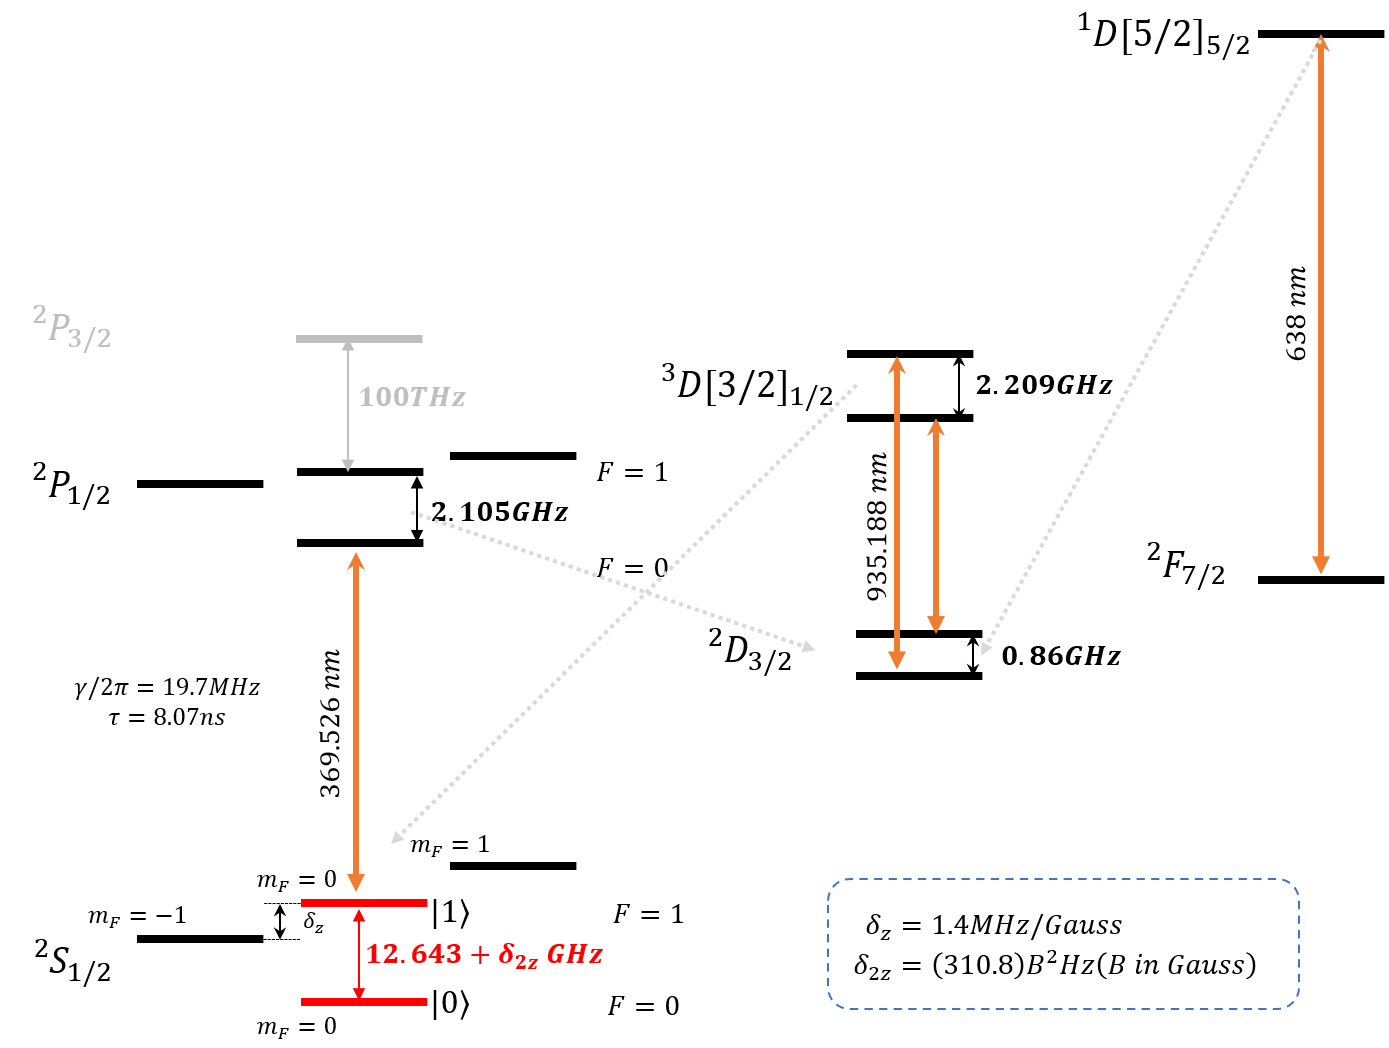
\includegraphics[width=1.0\linewidth]{energy_structure}
\end{figure}

通过在阱外向阱中离子施加的约$6$高斯的静磁场会使离子产生约$11$Hz的二阶\emph{Zeeman}能级劈裂。从$\ket{1}$态向$^2P_{1/2}$能级跃迁回路的驱动波长在$369.526$nm附近,这个波段的激光有成熟的商业激光系统供应,同时对光纤传输也很友好。略有遗憾的是这个$\ket{1}{^2P}_{1/2}$跃迁回路并不是完全闭合的,因为存在从$^2P_{1/2}$到$^2D_{3/2}$的微弱态泄露,分支比约为$0.5$\%\cite[]{Olmschenk_Younge_Moehring_Matsukevich_Maunz_Monroe_2007}。不过这个可以通过使用一个带$3.07$GHz边带的$935$nm波长的激光来将泄露的态再回泵浦到整个回路中。另外,背景撞击可能导致离子跑到$^2F_{7/2}$使离子“熄灭”,这个可以通过一个$638$nm波长的激光器来克服,重新将离子“点亮”。值得注意的是,这个任务除了$638$nm波长的激光器可以完成外,$760$nm\cite[]{Huntemann_Okhapkin_Lipphardt_Weyers_Tamm_Peik_2012}、$355$nm\cite[]{Senko_2014}。另外,由于从$^2F_{7/2}$到$^3F[1/2]_{3/2}$的跃迁大部分共振在$375.856$nm波长上,因此$375$nm波长的激光也可以完成。

\subsection[镱离子的电离和囚禁]{镱离子的电离和囚禁}
为了能够研究离子的特性我们首先需要将离子电离并稳定地囚禁住。
离子的囚禁采用的是
% 如第\ref{section:ion_classical_motion}节中介绍的
动态囚禁的方式,离子的电离一般是通过激光电离的方式实现的。对于$Yb^+$离子来说,电离的方式是采用的是\emph{两步电离法(two-step ionization)}\cite[]{Olmschenk_Younge_Moehring_Matsukevich_Maunz_Monroe_2007},这种方法可以避免紫外激光的使用。
首先,我们使用$398.991$nm波长的激光将镱原子重$^1S_0$能级激发到$^1P_1$能级;然后再使用一个低于$394.088$nm波长的激光将最外层电子激发到连续态区域中去,比如通常采用的$369.526$nm波长激光,或者$355$nm波长、$375$nm波长。在实践中,镱原子一般填充在原子炉中并被放置在真空室中。需要激发时就通过施加恒定电流加热原子,使原子从原子炉中热喷射出来的,其中会有一小部分穿过离子阱的中心。$398.911$nm和$369.525$nm波长的激光束在离子阱中心与原子炉中喷射出的原子重叠。于是,该区域的原子就可以被电离,并在高效冷却后被离子阱动态囚禁。由于同位素位移,我们可以通过微调$398.911$nm激光的波长来选择性地电离镱离子不同的同位素。为了抑制多普勒频移的影响,激光器的路径最好垂直于原子流。

\begin{figure}
    \centering
    \caption[刀片阱实物图]{实验中刀片阱实物图\label{fig:trap_blads}}
    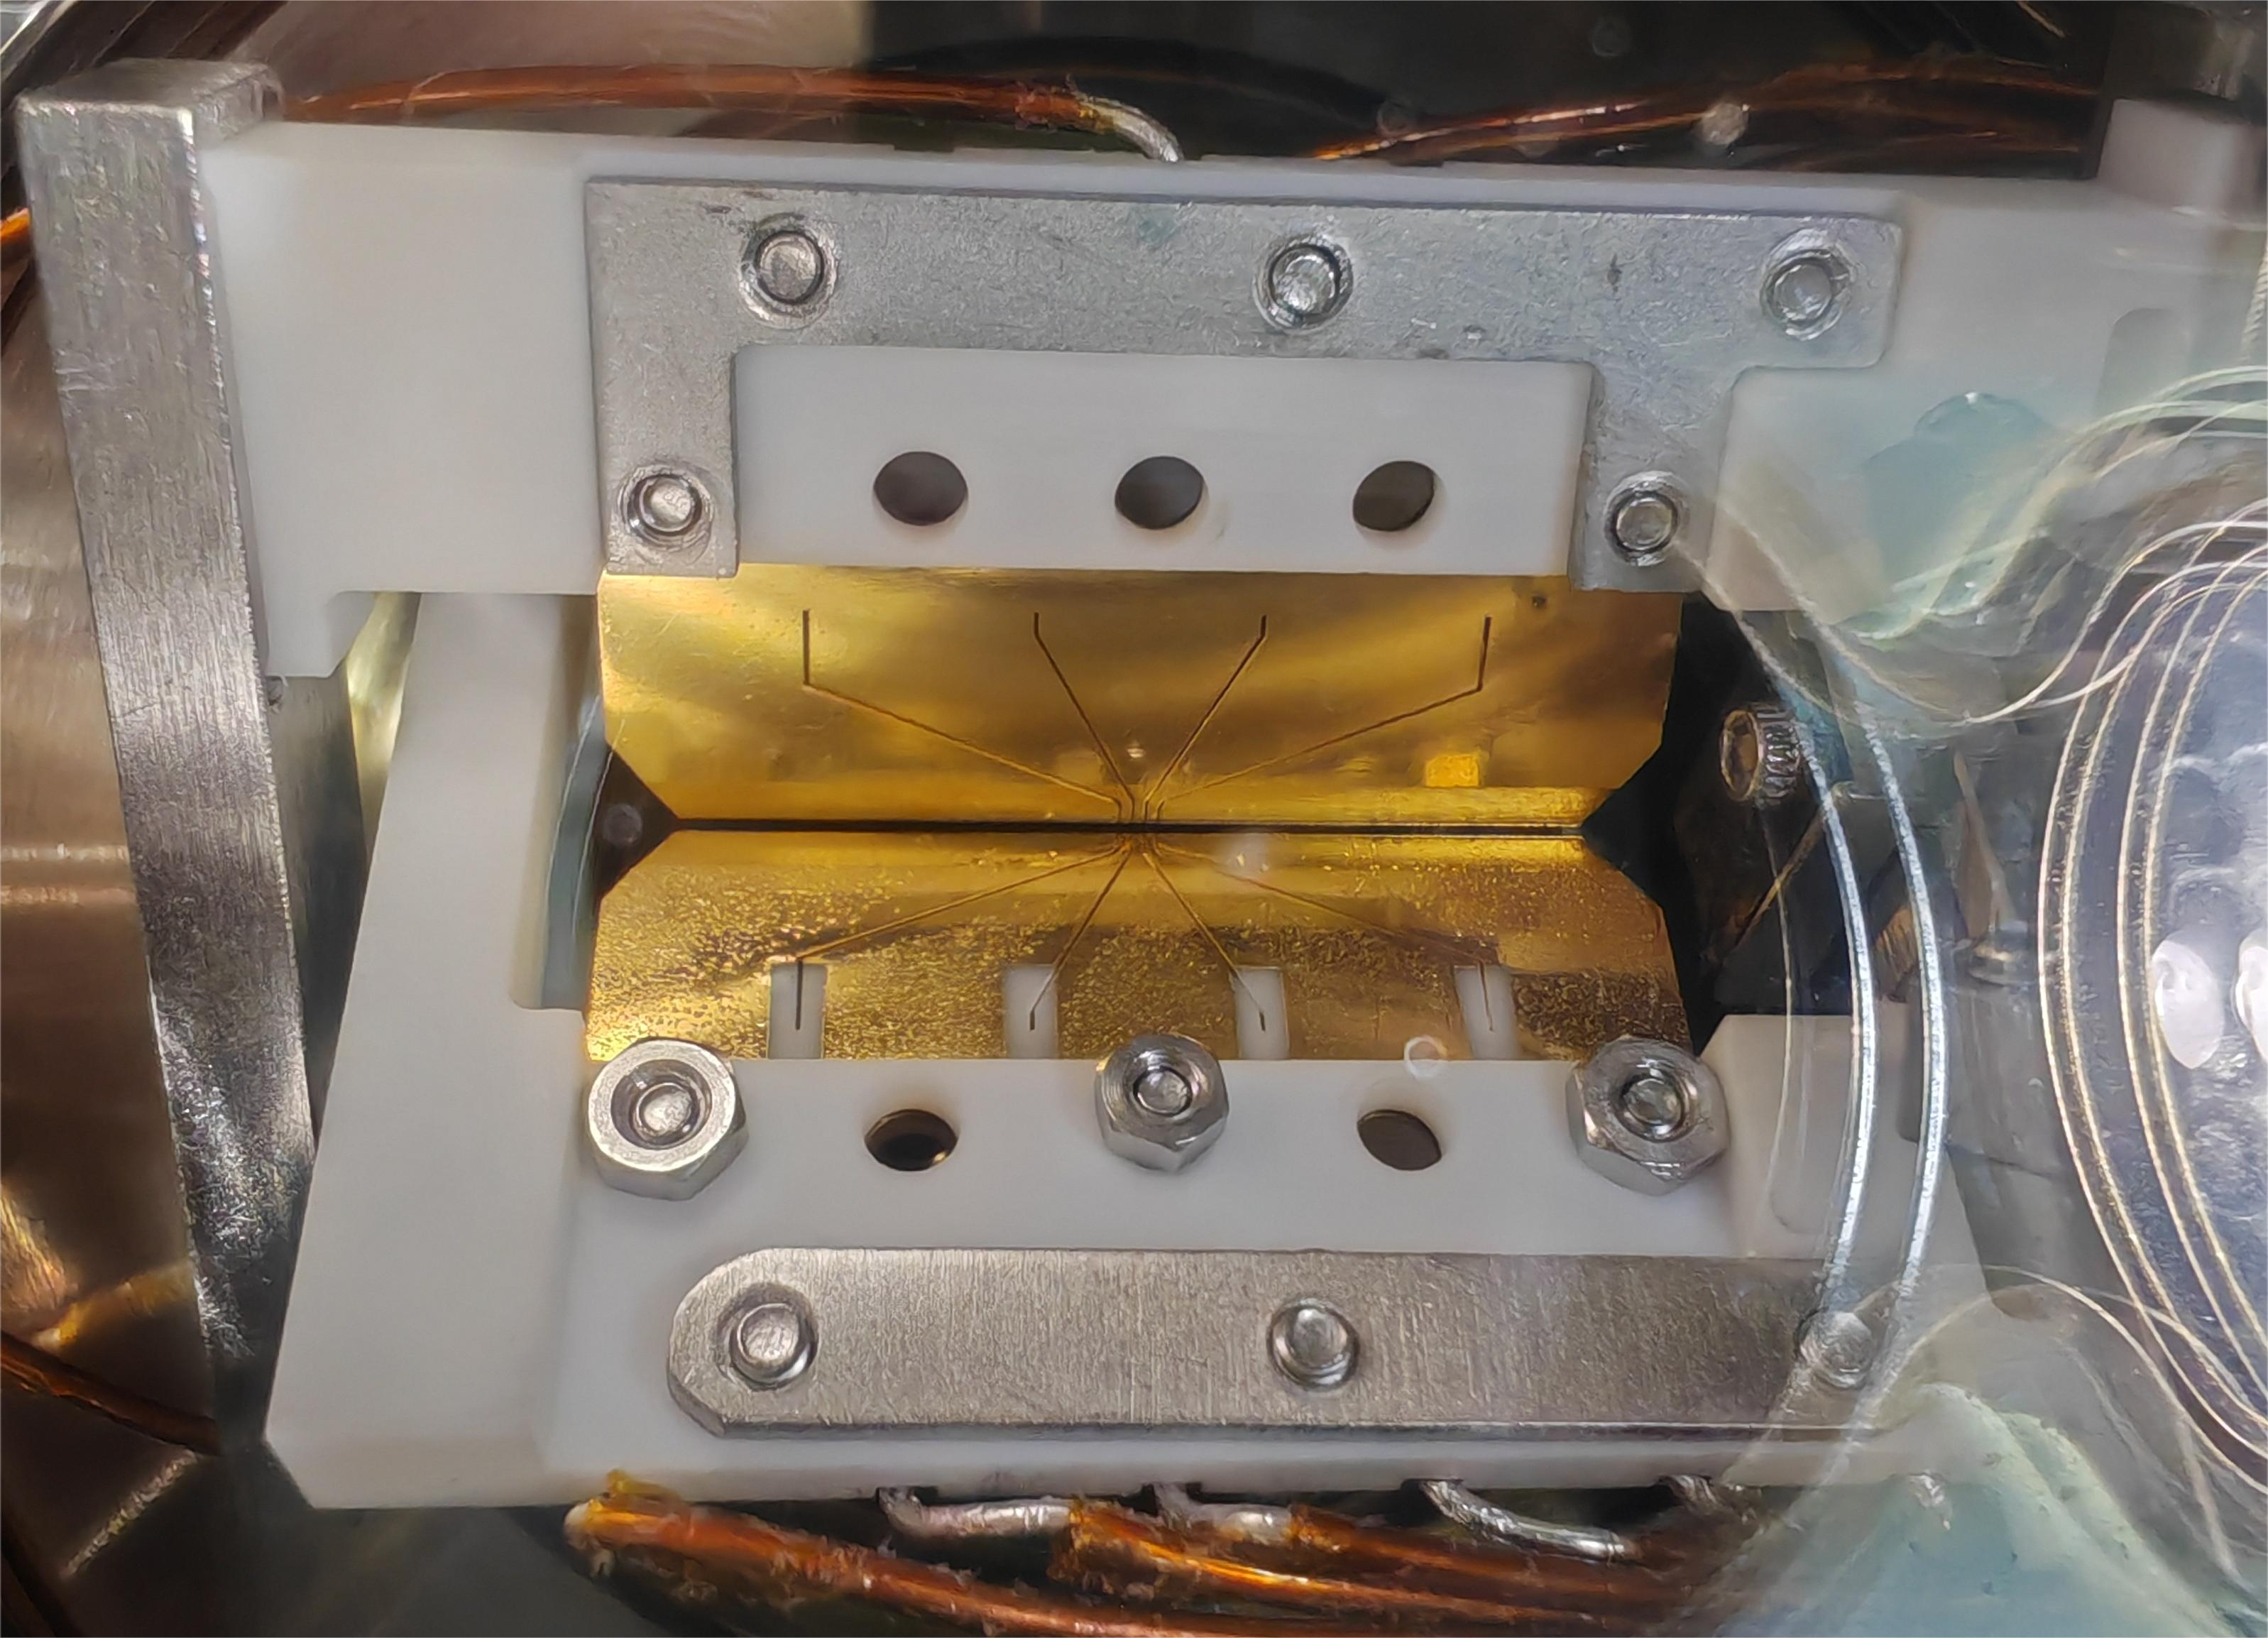
\includegraphics[width=0.8\linewidth]{trap_blads.jpg}
\end{figure}

% 如第\ref{section:ion_classical_motion}节中给介绍的,
由\emph{Earnshaw's theorem}\cite[]{Earnshaw}我们知道离子没有办法被静态地囚禁在三维空间中,好在我们仍然可以动态地将离子囚禁。实际实验中囚禁离子的离子阱如\ref{fig:trap_blads}图所示,这中类型的离子阱一般被称为刀片阱。它会产生如下形式的赝势$\Phi_p$:
\begin{align}
    \Phi_p=\frac{eV^2}{4MR^4\Omega_{rf}^2}\sum_{m}^{}\alpha_m^2r_m^2
\end{align}

其中$V$,$R$,$M$分别是RF电压、电极到阱中心的距离和离子的质量。$\Omega_{rf}$是RF的频率,$\alpha_m$是$r_m$方向的系数。
这个电势的结果是在所有方向上都有正的系数 ($\alpha_m^2>0$),直观地揭示了囚禁带电离子的能力。同时还可以从中得到有效的阱频率$\nu_m=eV\alpha_m/\sqrt{2}MR^2\Omega_{rf}$。

\subsection[镱离子的激光冷却]{镱离子的激光冷却\label{section:yb_laser_cooling}}
从原子炉中喷出的原子是十分“热”的(标准大气压下原子的平均融化温度高达$824 ^o C$),由麦克斯韦运动分布可知它们的速度能达到超过一百米每秒。如此热的电子很容易从离子阱的囚禁电势中逃脱,很难被囚禁更不用说进行什么别的操作了。因此,我们需要某种冷却手段来给离子“降温”。

\begin{figure}
    \centering
    \caption[激光施加到离子的多普勒效应示意图]{激光施加到离子的多普勒效应示意图\label{fig:doppler_cooling_scattering}}
    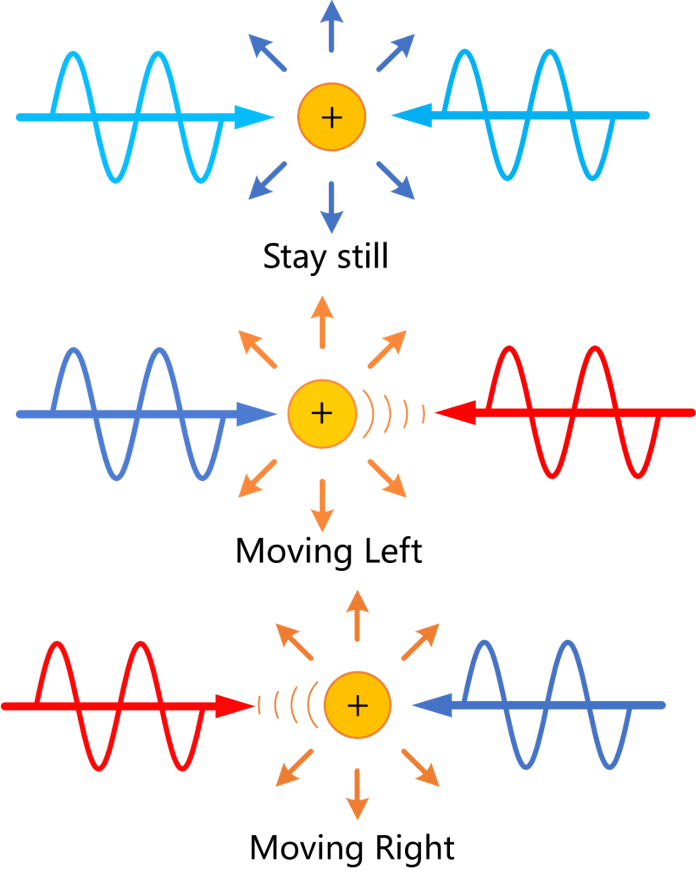
\includegraphics[width=0.45\linewidth]{doppler_cooling_scattering}
\end{figure}
离子可以使用红色失谐的反向传播激光束进行激光冷却,这被称为多普勒冷却\cite[]{Hänsch_Schawlow_1975}。如图\ref{fig:doppler_cooling_scattering}所示,当离子与激光反向运动时,吸收一个光子离子将减少$\hbar \vec{k}$的动量;当离子与光同向运动时,吸收一个光子离子将增加$\hbar \vec{k}$的动量。随后离子将通过受激辐射的形式随机散射$\hbar \vec{k}$的动量,这个随机散射过程的平均结果是动量变化为$0$。

\begin{figure}
    \centering
    \caption[多普勒冷却示意图]{多普勒冷却示意图\label{fig:doppler_cooling}}
    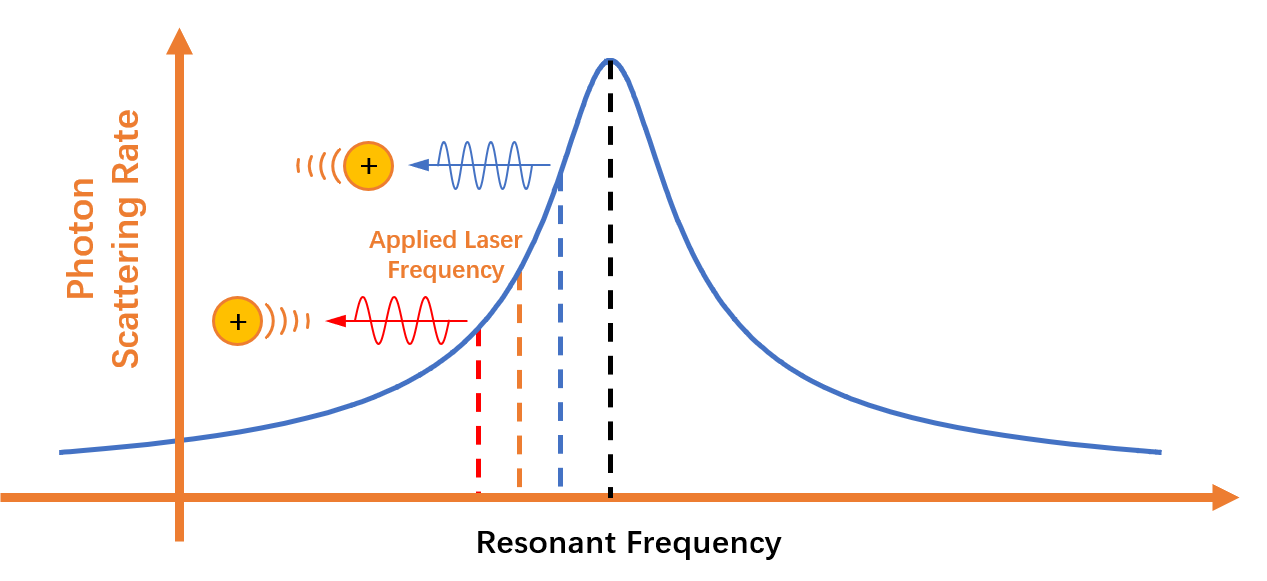
\includegraphics[width=1.0\linewidth]{doppler_cooling}
\end{figure}
如图\ref{fig:doppler_cooling}所示,由于多普勒效应,在离子局部坐标系下看入射激光的波长会产生$-\vec{k}\cdot\vec{v}$的频移。因此如果施加红是失谐的激光,那么与激光方向相反的离子将比与激光方向相同的离子吸收更多的光子;另一方面,对打的激光会抵消激光本身对离子的加速效应,最终离子会失去较多的动量,被激光“冷却”下来。

对$Yb^+$离子来说,在这个过程中跃迁$^2S_{1/2}\ket{F=1}\to {^2P}_{1/2}\ket{F=0}$和$^2S_{1/2}\ket{F=0}\to {^2P}_{1/2}\ket{F=1}$同时被驱动以覆盖离子的所有超精细能级,避免离子陷入暗态(变黑)。
此外,冷却激光的所有偏振都施加上去来提高冷却效率,相关跃迁回路和离子散射图如图\ref{fig:doppler_cooling_level}所示。
\begin{figure}
    \centering
    \caption[离子冷却跃迁回路示意图]{离子冷却跃迁回路示意图\label{fig:doppler_cooling_level}}
    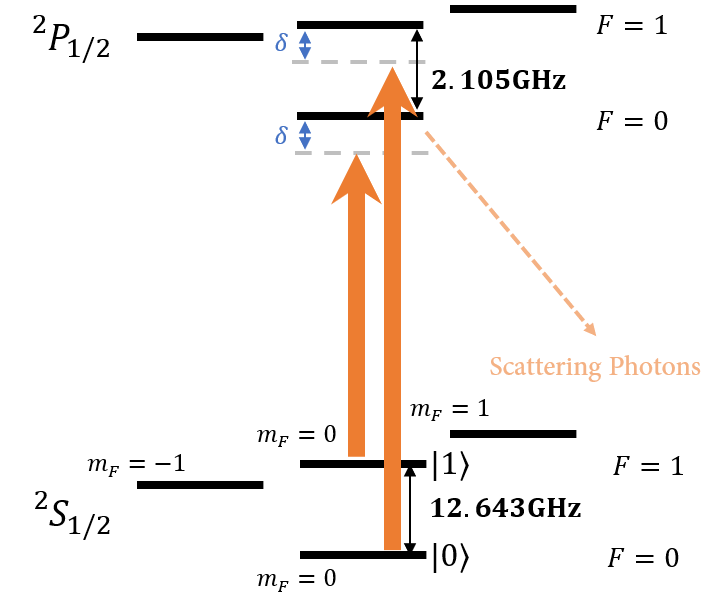
\includegraphics[width=0.6\linewidth]{doppler_cooling_level}
\end{figure}

\subsection[镱离子的态初始化]{镱离子的态初始化\label{section:yb_state_init}}

几乎任何量子计算或模拟任务都以确定性的纯状态开始。获得这个起点的过程称为\emph{态初始化(State Initialization)},这是通过囚禁离子平台中的光泵浦过程实现的。

\begin{figure}
    \centering
    \caption[离子态初始化示意图]{离子态初始化示意图\label{fig:initialization}}
    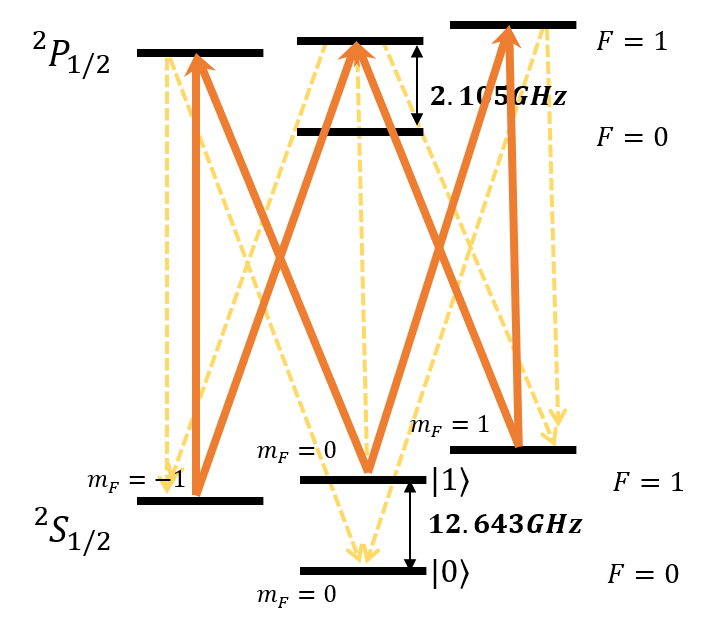
\includegraphics[width=0.6\linewidth]{initialization}
\end{figure}

如图\ref{fig:initialization}所示,在初始化过程中从$^2S_{1/2}\ket{F=1}$到$^2P_{1/2}\ket{F=1}$的跃迁被驱动。离子的状态很有可能衰减到$\ket{0}$状态,因此由于$12.6$GHz的失谐,处于$\ket{0}$态的离子不会参与进一步的激发。对于单个离子,这一过程在$5$μs内就可以以非常高的初始化保真度完成。这篇\cite[]{Harty_Allcock_Ballance_Guidoni_Janacek_Linke_Stacey_Lucas_2014}文献展示了状态初始化的误差小于可以$10^{−4}$。

\subsection[镱离子的态探测]{镱离子的态探测\label{section:yb_state_detection}}
在经过各种中间操控后,量子计算的结果需要被读出,这一过程通过离子的态测量实现。如图\ref{fig:detection}所示,通常采用状态相关的荧光检测技术进行高保真读出\cite[]{Blinov_Leibfried_Monroe_Wineland_2004}。在这个过程中使用的是$^2S_{1/2}\ket{F=0}$到$^2P_{1/2}\ket{F=1}$之间的跃迁($^2S_{1/2}\ket{F=0}$到$^2P_{1/2}\ket{F=0}$之间的跃迁是偶极禁止跃迁的)。因此,我们可以通过数收集散射光子的数量的多少来区分投影状态。
\begin{figure}
    \centering
    \caption[离子态测量示意图]{离子态测量示意图\label{fig:detection}}
    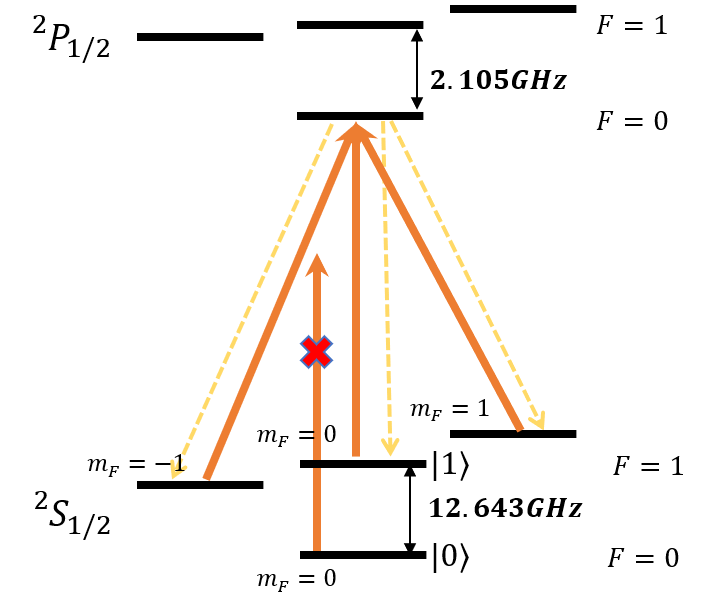
\includegraphics[width=0.6\linewidth]{detection}
\end{figure}

态测量过程得到的离子影像可以用\emph{电子倍增电荷耦合器件(Electron-multiplying charge-coupled device, EMCCD)}或者\emph{光电倍增管(Photomultiplier Tube, PMT)}通过两步成像来显示,如图\ref{fig:two_step_imaging}所示。
对于单个离子,为了量化量子比特状态检测的保真度,我们可以将量子比特准备为$\ket{0}$状态或$\ket{1}$状态,然后应用持续$40$μs的探测激光束同时计数收集到的光子。每个状态的序列通常重复$2000$次以获得统计分布。
以我们目前系统为例,入射光子数量的统计数据几乎遵循泊松分布,$\ket{0}$和$\ket{1}$状态的平均光子分别为$0.05$和$9.58$。分离良好的分布使我们能够将投影状态与固定阈值区分开来。对于单次检测,如果收集到的光子数大于1,则我们将投影状态分类为$\ket{1}$状态,否则投影状态被视为$\ket{0}$状态。

\begin{figure}
    \centering
    \caption[两步成像系统]{两步成像系统\label{fig:two_step_imaging}}
    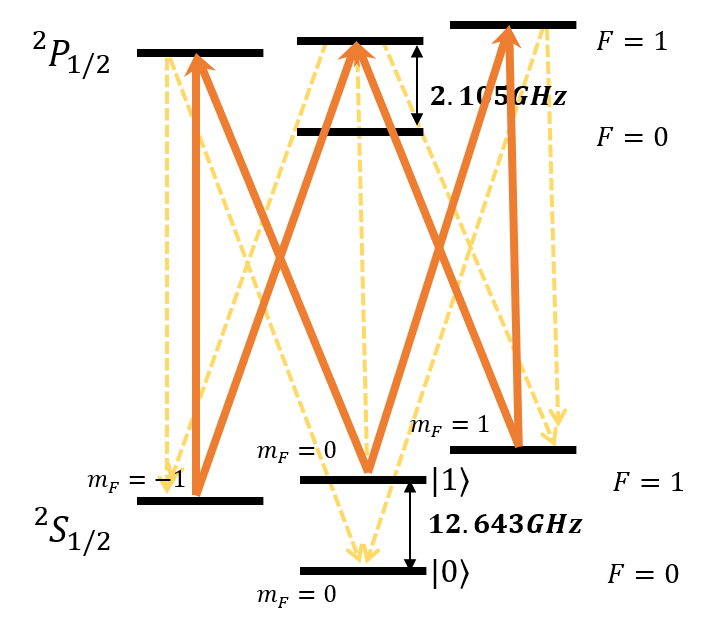
\includegraphics[width=0.6\linewidth]{two_step_imaging}
\end{figure}



\subsection[镱离子的态操控]{镱离子的态操控\label{section:yb_state_manipulation}}
离子量子比特可以通过微波\cite[]{Olmschenk_Younge_Moehring_Matsukevich_Maunz_Monroe_2007}或脉冲激光\cite[]{Lee_2005}实现。微波对离子的态操控实现简单,但是由于所用微波的长波太长,使用微波技术方案往往仅限于单比特门;激光操控离子有诸多优点,尤其是在大规模的集成和寻址方面。接下来的小节将具体介绍这两类离子比特门操控方式。
\subsubsection[微波操控镱离子]{微波操控镱离子\label{section:microwave_operation}}
本小节将简要介绍微波操控的离子量子门,以帮助建立离子态操控的一般方式。
在微波场下的离子哈密顿量为(保持$\hbar=1$):
\begin{align}
    \hat{H}=\frac{\omega_q}{2}\hat{\sigma}_z + \Omega\cos\left(\vec{k}\cdot\vec{r}-\omega t + \phi\right)\hat{\sigma}_x
\end{align}

第一项是简化的离子比特二能级系统的希尔伯特空间,其能量差为$\omega_q$;第二项是磁偶极跃迁的导出项,其中磁场的振动频率为$\omega$,初始相位为$\phi$;$\Omega$是代表耦合强度的拉比频率;当$\omega\approx 12.6$GHz时有$\vec{k}\approx3\times ^{-4}um^{-1}$,所以空间项$\vec{k}\cdot \vec{r}$相对比较小,可以被忽略。通过一个重映射变换$\hat{H}_I=e^{iH_0t}(\hat{H}-\hat{H}_0)e^{-iH_0t}$,其中$\hat{H}_0=\omega\hat{\sigma}_z/2$,可以将自由空间哈密顿量转化到相互作用表象(dressed-state)下:
\begin{align}
    \hat{H}_I&=e^{iH_0t}(\hat{H}-\hat{H}_0)e^{-iH_0t}\\
    &=-\frac{\mu}{2}\hat{\sigma}_z+\frac{\Omega}{2}\left(\hat{\sigma}_+e^{i\omega t}+\hat{\sigma}_-e^{-i\omega t}\right)\left(e^{i(\omega t-\phi)}+e^{-i(\omega t-\phi)}\right)\\
    &\approx -\frac{\mu}{2}\hat{\sigma}_z+\Omega(\hat{\sigma}_+e^{i\phi}+\hat{\sigma}_-e^{-i\phi})\\
    &=-\frac{\mu}{2}\hat{\sigma}_z+\frac{\Omega\cos{\phi}}{2}\hat{\sigma}_x+\frac{\Omega\sin{\phi}}{2}\hat{\sigma}_y\label{eq:interaction_hamiltonian_microwave}
\end{align}

其中$\mu=\omega=\omega_q$是量子比特和单微波光子之间的能量差。在$\approx$这步,我们采用了在第\ref{section:coupling_theory}节中介绍过的\emph{旋波近似},将含$2\omega$的快速振动项忽略掉了。相互作用表象(dressed-state)的优点在于最终的哈密顿量是不含时的,这样各个泡利矩阵的成分的概率幅就完全由施加的微波场决定了。
对于一个给定的状态$\ket{\Psi(0)}=c_0(0)\ket{0}+c_1(0)\ket{1}$,其中$|c_0(0)|^2+|c_1(0)|^2=1$,它的时间演化由演化算符$U(t)$决定:
\begin{align}
    \ket{\Psi(t)}=U(t)\ket{\Psi(0)}=\exp(-iH_It)\ket{\Psi(0)}
\end{align}

如果给定$\ket{\Psi(0)}=\ket{0}$,那么可以解析地写出这个态的演化后的概率幅:
\begin{align}
    c_1(t)&=-i\frac{\Omega}{\Omega_{eff}}e^{i\phi}\sin{\frac{\Omega_{eff}t}{2}},\\
    c_0(t)&=\cos{\frac{\Omega_{eff}t}{2}}-i\frac{\mu}{\Omega_{eff}}\sin{\frac{\Omega_{eff}t}{2}}
\end{align}

其中$\Omega_{eff}=\sqrt{\Omega^2+\mu^2}$是有效拉比频率\cite[]{Foot_2005}。$\ket{1}$态的概率$p_1(t)=|c_1(t)|^2$在时间$t=\pi/\Omega_{eff}$时取得最大值,最大值为$\Omega^2/(\Omega^2+\mu^2)$。不同失谐$\mu$情况下的拉比振荡如图所示。

\begin{figure}
    \centering
    \caption[不同失谐$\mu$情况下的拉比振荡]{不同失谐$\mu$情况下的拉比振荡\cite[]{Lu_2019}}
    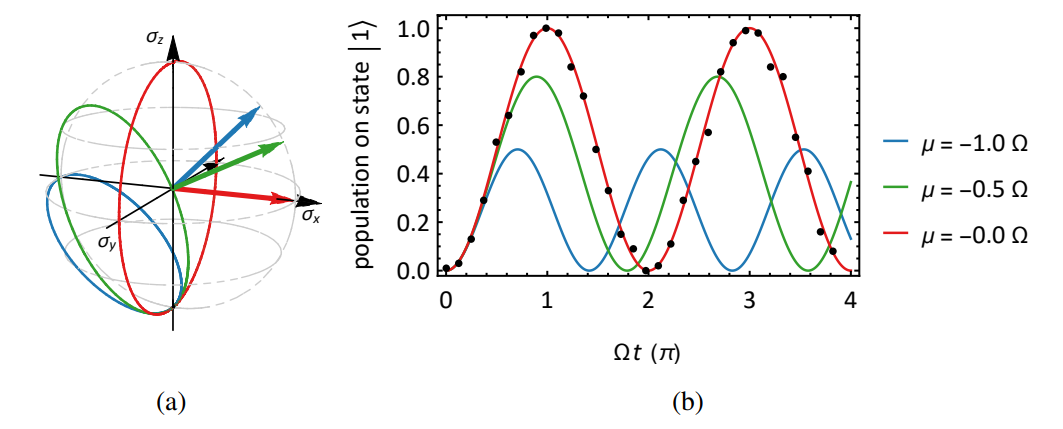
\includegraphics[width=1.0\linewidth]{rabi_oscillations}
\end{figure}

在量子计算的实现中,我们总是使$\mu\approx0$以实现任意单比特的旋转操控:
\begin{align}
    R_\phi(\theta)=U\left(\frac{\theta}{\Omega},P\phi\right)=\exp[-i\frac{\theta}{2}\sigma_\phi]
\end{align}

其中$\sigma_\phi=\sigma_x\cos{\phi}+\sigma_y\sin{\phi}$。对于初始状态,在$\theta=\pi$或者说是$t=\pi/\Omega$时,初始态的概率可以完全转移到二能级系统的另一个态上。这种$R_\phi(\theta)$旋转操作被称为沿着$\phi$轴的态旋转操控,$R_\phi(\pi)$被称为$\pi$翻转,它的作用类似经典的NOT门。除此之外,还有一种重要的旋转操作$R_\phi(\pi/2)$,它常被称为$\pi/2$翻转,可以用来制备十分有用的叠加态$(\ket{0}+e^{-i\phi}\ket{1})/\sqrt{2}$。



\subsubsection[连续激光操控镱离子]{连续激光操控镱离子\label{section:raman_transition}}

离子的内态也可以用激光通过称为\emph{受激拉曼跃迁(Stimulated Raman Transition, SRT)}的过程来操控。与微波场操控的方式相比,光学激光器的波长更短,提供了强大量子比特寻址的优势,这对于多量子比特情况下的单个量子比特操作至关重要,接下来的部分介绍了这种方法。


信息储存在镱离子的超精细能级上,$\ket{0}$和$\ket{1}$能级之间有着$12.6$GHz的能量差。尽管激光的能量远大于这个能级间隔以至于无法用激光直接操控$\ket{0}$态和$\ket{1}$态之间的跃迁,我们仍然可以通过两光子的受激拉曼跃迁来实现对离子内态的操控,如图\ref{fig:raman_transition}所示。
通过同时激发从$\ket{0}$和$\ket{1}$到一个中间激发态$\ket{e}$的电偶极跃迁,整个系统的自由空间哈密顿量可以写为:
\begin{align}
    \hat{H}&=\frac{\omega_q}{2}\hat{\sigma}_z+\left(\omega_e+\frac{\omega_q}{2}\right)\ket{e}\bra{e}\\
    &+\frac{\Omega_1}{2}(\ket{e}\bra{0}+\ket{e}\bra{1}+H.c.)\left(e^{i(\vec{k}_1\cdot\vec{r}-\omega_1t+\phi_1)}+H.c.\right)\\
    &+\frac{\Omega_2}{2}(\ket{e}\bra{0}+\ket{e}\bra{1}+H.c.)\left(e^{i(\vec{k}_2\cdot\vec{r}-\omega_2t+\phi_2)}+H.c.\right)
\end{align}

\begin{figure}
    \centering
    \caption[镱离子受激拉曼跃迁示意图]{镱离子受激拉曼跃迁示意图。$\ket{e}$:上级激发态能级;$\ket{0},\ket{1}$:编码量子信息的高低能级;$\omega_{q}$:编码量子信息的能级能隙;$\Delta$:激光相对于上级激发态能级的失谐;$\mu$:用于施加数态跃迁的失谐;$\omega_e$:$\ket{1}$和$\ket{e}$能级的能隙;$\omega_1,\phi_1,\vec{k}_1, \Omega_1$和$\omega_2,\phi_2,\vec{k}_2, \Omega_2$:施加到离子量子信息编码能级上的激光频率、相位、波矢、耦合强度等参数。\label{fig:raman_transition}}
    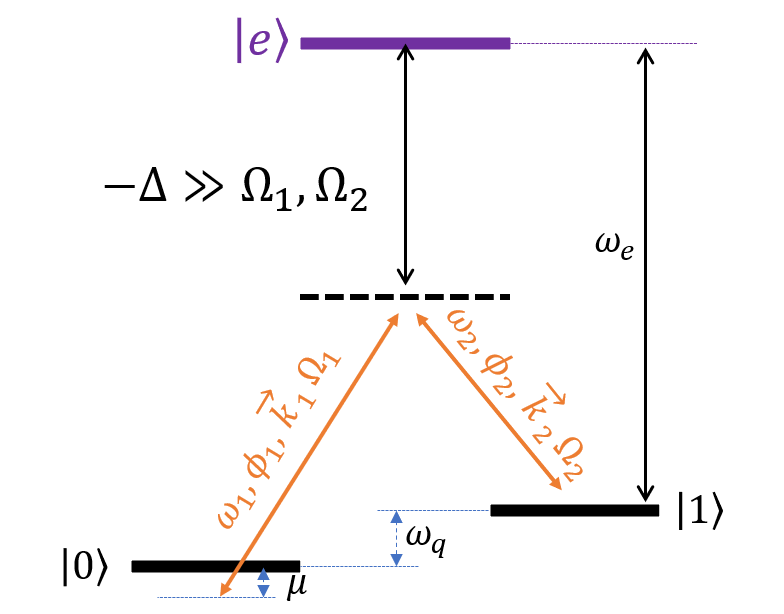
\includegraphics[width=0.6\linewidth]{raman_transition}
\end{figure}

其中$\Omega_i,\vec{k}_i, \phi_i$分别为第$i$个拉曼激光的电偶极跃迁强度、波矢和光相位。$H.c.$表示厄米共轭。如果在旋转坐标系$\hat{H}_0=\frac{\omega_1\hat{\sigma}_z}{2}+\left(\omega_e+\frac{\omega_q}{2}\right)\ket{e}\bra{e}$下看,相互作用的哈密顿量变为了:
\begin{align}
    \hat{H}=
    &\left(\frac{\Omega_1}{2}e^{i(-\Delta-\mu)t}e^{i(\vec{k}_1\cdot \vec{r}+\phi_1)}
    +\frac{\Omega_2}{2}e^{i(-\Delta+\omega_q)t}e^{i(\vec{k}_2\cdot \vec{r}+\phi_2)}\right)\ket{e}\bra{0}\\
    +&\left(\frac{\Omega_1}{2}e^{i(-\Delta-\mu-\omega_q)t}e^{i(\vec{k}_1\cdot \vec{r}+\phi_1)}
    +\frac{\Omega_2}{2}e^{i(-\Delta)t}e^{i(\vec{k}_2\cdot \vec{r}+\phi_2)}\right)\ket{e}\bra{1}+H.c.\label{eq:interaction_hamiltonian_yb}
\end{align}

其中失谐$-\Delta$如图\ref{fig:raman_transition}所示.考虑$\Delta\gg\Omega_1,\Omega_2$且$|\Delta|\gg\omega_q\gg\mu$的情况,这时中间激发态$\ket{e}$可以绝热消除,最终离子比特系统中有效的哈密顿量如下:
\begin{align}
    \hat{H}_{eff}=\frac{\delta_{diff}}{2}\hat{\sigma}_z+\frac{\Omega}{2}\left(\hat{\sigma}_+e^{i\left(\vec{k}\cdot\vec{r}-\mu t+\phi\right)}
    +\hat{\sigma}_-e^{-i\left(\vec{k}\cdot\vec{r}-\mu t+\phi\right)}\right)\label{eq:effective_hamiltonian_raman}
\end{align}

其中$\Omega=\frac{\Omega_1\Omega_2}{2\Delta}$,$\vec{k}=\vec{k}_1-\vec{k}_2$,$\phi=\phi_1-\phi_2$分别是有效拉比频率、有效波矢和激光的相对相位。$\delta_{diff}$有如下形式\cite[]{James_Jerke_2007}:
\begin{align}
    \delta_{diff}&=-\left(\frac{\Omega_1^2}{4(-\Delta-\mu-\omega_q)+\frac{\Omega_2^2}{4(-\Delta)}}\right)+\left(\frac{\Omega_1^2}{4(-\Delta+\mu)+\frac{\Omega_2^2}{4(-\Delta+\omega_q)}}\right)\\
    &\approx-\frac{\Omega_1^2+\Omega_2^2}{4\Delta}\frac{\omega_q}{\Delta}
\end{align}

这个是量子比特能级的差分光位移,由于在一般的实验设置中$\omega_a/|\Delta|\sim 10^{-3}\ll 1$,$\delta_{diff}$的值非常小。这项可以通过将原来的旋转坐标$\omega_q$重新选择为$(\omega_q+\delta_{diff})$来吸收掉。
另外注意,这里的有效哈密顿量与公式\eqref{eq:interaction_hamiltonian_microwave}的共振情况相同,后者是用微波进行的操控。因此如果我们让$\vec{k}_1=\vec{k}_2$且$\mu=\delta_{diff}\approx0$,那么这两种离子比特的操控方式从结果上看没有什么不同。不过实际上,两者还有所不同。除了上面提高过的受激发的拉曼跃迁方法有单比特寻址的能力外,它还通过改变传播拉曼光束的角度$\vec{k}\in[0,4\pi/\lambda]$(激光方向从同向到反向传播)来提供波矢$\vec{k}$的操控自由度。因为波长$\lambda$是在光学波段,最大的波矢模$|\vec{k}|$能达到$10um^{-1}$,这为离子的运动耦合提供了可能性。离子也可以看作是一个以频率$\nu$振动的量化的谐振子
% (第\ref{section:ion_classical_motion}节)
,这时公式\eqref{eq:effective_hamiltonian_raman}中的哈密顿量为:
\begin{align}
    H_{eff}=\nu a^\dagger a+\frac{\Omega}{2}\left(\sigma_+e^{i(\eta(a^\dagger a)-\mu t+\phi)}+H.c.\right) \label{eq:effective_hamiltonian_rotating}
\end{align}

其中$a,a^\dagger$分别是产生和湮灭算子。这里我们通过研究一个维度的情况来具体说明,比如$x$方向。此时$\vec{k}\cdot\vec{r}\to k\cdot x$等价于$k\Delta x(a+a^\dagger)=\eta(a+a^\dagger)$,其中$\Delta x=\sqrt{\hbar/2M\nu}$是基态波函数的拓展,$\eta=k\Delta x$是在第\ref{section:coupling_theory}节介绍过的LDP。将公式\eqref{eq:effective_hamiltonian_rotating}转换到$H_0=\nu a^\dagger a$的表象下并将$\exp{i\vec{k}\cdot \vec{r}}$进行一阶展开,可以得到近似的相互作用哈密顿量:
\begin{align}
    H_I\approx\frac{\Omega}{2}\left[\sigma_+(1+i\eta a e^{-i\nu t}+i\eta a^\dagger e^{i\nu t})e^{-i\mu t+i\phi}+H.c.\right]
\end{align}

这个近似形式仅在$\eta\sqrt{\braket{(a+a^\dagger)^2}}\ll1$时成立,这也被称为\emph{Lamb-Dick近似(Lamb-Dick Approximation)},其中$\braket{\cdot}$表示量子态平均。在实验中这个条件是成立的,不然就会产生高阶的跃迁。通过调节$\mu$等于$0,-\nu,\nu$,我们可以得到三种类型的跃迁:
\begin{align}
    H_{car}&=\frac{\Omega}{2}(\sigma_+e^{i\phi}+H.c.)\\
    H_{rsb}&=\frac{i\eta\Omega}{2}(\sigma_+ae^{i\phi}+H.c.)\\
    H_{bsb}&=\frac{i\eta\Omega}{2}(\sigma_+a^\dagger e^{i\phi}+H.c.)
\end{align}

$H_{car}$, $H_{rsb}$, $H_{bsb}$分别被称为载带跃迁、红边带跃迁和蓝边带跃迁,如图\ref{fig:red_carray_blue_sideband}所示。离子比特的两个内能级分别为$\ket{0},\ket{1}$;灰色先表示载带跃迁,其拉比频率为$\Omega$;红色线和蓝色线分别表示红边带和蓝边带跃迁,相应的拉比频率为$\eta \Omega$;$\nu$表示两个数态之间的能隙,也就是实现红蓝边带跃迁需调节的失谐量。

\begin{figure}
    \centering
    \caption[载带跃迁、红边带跃迁和蓝边带跃迁示意图]{载带跃迁、红边带跃迁和蓝边带跃迁示意图。$\ket{0},\ket{1}$:编码量子信息的高低能级;$\Omega$:驱动激光耦合强度;$\eta \Omega$:数态跃迁的耦合强度;$\nu$:数态之间的失谐能隙;$\ket{0}_F,\ket{1}_F,\ket{2}_F,\dots$:不同的数态的编号。\label{fig:red_carray_blue_sideband}}
    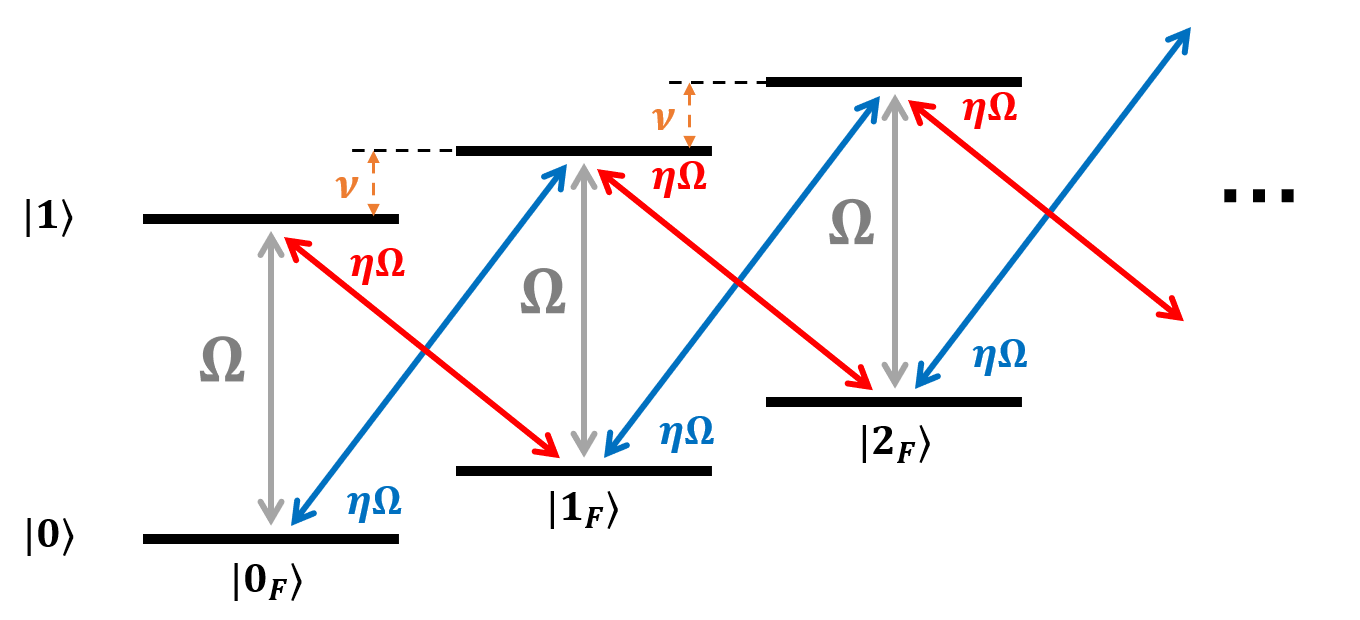
\includegraphics[width=0.8\linewidth]{red_carray_blue_sideband}
\end{figure}

载带跃迁可以用来实现如微波操控一样(第\ref{section:microwave_operation}节)的单比特门翻转$R_\phi(\theta)$。
红边带跃迁和蓝边带跃迁的哈密顿量分别称为\emph{Jaynes-Cummings}或\emph{anti-Jaynes-Cummings}模型\cite[]{Karnieli_Fan_2023}。这类跃迁可以将量子比特与其外部量化运动耦合,这对于实现多个离子量子比特纠缠至关重要。


\subsubsection[脉冲激光操控镱离子]{脉冲激光操控镱离子\label{section:pulsed_laser_ion_operation}}
如上一节所述的在用激光操控离子的技术方案下,$\ket{0}$和$\ket{1}$态耦合的主要方式是通过受激拉曼跃迁。脉冲激光控制离子的原理本质上与连续激光的情况没有不同。主要区别在于连续激光是通过驱动拉曼跃迁来控制的,而脉冲激光是通过同时驱动一系列小间隔的拉曼跃迁来控制的。原理图如图\ref{fig:pulsed_laser_interaction}所示。
\begin{figure}
    \centering
    \caption[脉冲激光操控镱离子]{脉冲激光操控镱离子。$\ket{0},\ket{1}$:编码量子信息的高低能级;$\omega_R$:激光重复频率间隙;$\omega_q$:编码量子信息的能级能隙;$\omega_0$:脉冲激光中心频率;$\Delta$:与上级激发态能级的失谐量。\label{fig:pulsed_laser_interaction}}
    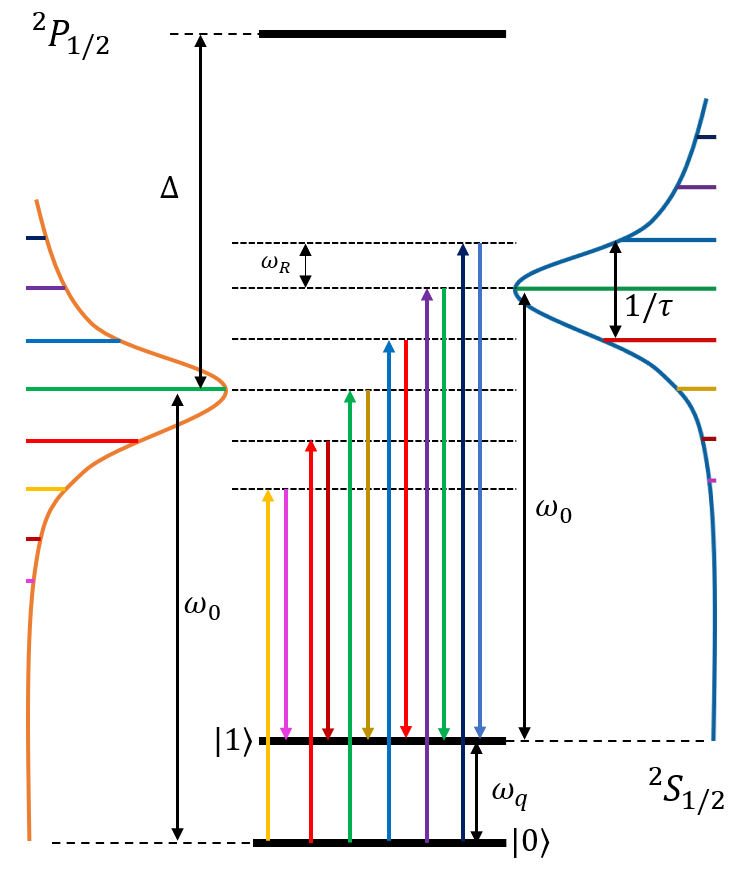
\includegraphics[width=0.8\linewidth]{pulsed_laser_interaction}
\end{figure}

在空间中的固定点上,理想化的激光脉冲束有一个时间独立的电场$E(t)$:
\begin{align}
    E(t)=\sum_{n=1}^{N}f(t-nT)e^{i\omega_0t}
\end{align}

其中$f(t)$是脉冲激光的包络,$T$是激光脉冲的重复周期,$N
$是整数激光包含的脉冲数,$\omega_0$是脉冲激光的波长。脉冲激光在频域中可以表示为:
\begin{align}
    E(\omega)=\sum_{n=0}^{\infty}\tilde{f}(\omega)(\omega_0\pm n\omega_R)
\end{align}

其中$\tilde{f}(\omega)=\mathcal{F}(f(t))$表示$f(t)$傅里叶变换的结果,$\omega_R=2\pi\nu_R$是脉冲激光的重复频率。如图\ref{fig:pulsed_laser_comb}所示,脉冲激光在频域上是一些列频率梳齿,离子比特态之间拉曼跃迁的共振拉比频率由梳齿的所有谱分量的总和给出,如图\ref{fig:pulsed_laser_interaction}所示。在绝热近似消除激发态$^2P_{1/2}$并执行旋转波近似后,脉冲激光的受激拉曼跃迁拉比频率有以下形式\cite[]{Hayes_Matsukevich_Maunz_Hucul_Quraishi_Olmschenk_Campbell_Mizrahi_Senko_Monroe_2010}:
\begin{align}
    \Omega=\frac{|\mu|^2\sum_{l}^{}E_lE_{l-q}}{\Delta}\approx\Omega_0\left(\frac{\omega_q\tau}{e^{\frac{\omega_q\tau}{2}}-e^{-\frac{\omega_q\tau}{2}}}\right)
\end{align}

\begin{figure}
    \centering
    \caption[脉冲激光在频域中的梳齿]{脉冲激光在频域中的梳齿\cite[Chap1.3]{Mizrahi_2013}\label{fig:pulsed_laser_comb}}
    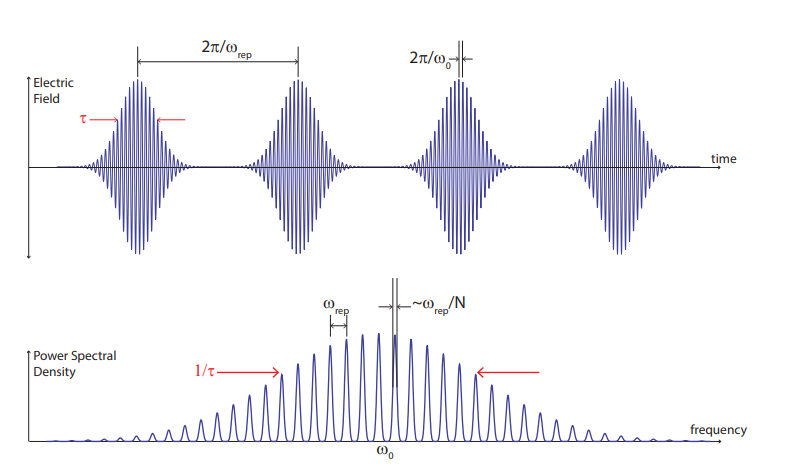
\includegraphics[width=1.0\linewidth]{pulsed_laser_comb}
\end{figure}

其中$\mu$是地面之间的偶极子矩阵元素,$\tau\approx 1 psec$是每个脉冲的持续时间,$E_k\equiv \nu_R\tilde{f}(2\pi k\nu_R)$是激发态电子态,$q\equiv\omega_q/\omega_R$是整数。在上述的近似表述中,求和被表述为积分,每个脉冲表示为$f(t)=\sqrt{\pi/2}E_0 sech(\pi t/\tau)$($\tau\ll T$)。$\Omega_0=\nu_R\tau|\nu E_0|^2/\Delta=s\gamma^2/2\Delta$脉冲束的时间平均谐振拉比频率,$\gamma/2\pi=20MHz$是$^2P_{1/2}$态的辐射线宽,$s=\bar{I}/T_{sat}$是$^2S_{1/2}\leftrightarrow ^2P_{1/2}$的饱和强度。在假设单脉冲带宽与我们的实验系统中满足的超精细频率($\omega_q\tau\ll 1$)相比较大的情况下,可以得到$\Omega\approx\Omega_0$。








% \section[Mølmer-Sørensen 门]{Mølmer-Sørensen 门}
\section[基于离子的通用量子门]{基于离子的通用量子门}

通用量子门是构建量子计算机的基本单元,它可以通过组合和嵌套来实现各种量子计算操作,如量子比特的翻转、量子态的制备和测量等,想要实现离子量子计算就需要用离子比特构建通用量子门。两比特纠缠门可以通过利用不同离子之间共享的集体运动实现。该策略利用了囚禁离子链的一个非常有利的特性,称为\emph{完全连通性(Full Connectivity)},这意味着整个离子链的离子都有相互作用。

Ignacio Cirac和Peter Zoller最早在1995年中提出了双量子比特纠缠门的第一个方案\cite[]{Cirac_Zoller_2002},称为\emph{Cirac-Zoller门(Cirac-Zoller Gate, CZ-Gate)},并在2003年在实验中实现\cite[]{Schmidt_Kaler_Häffner_Riebe_Gulde_Lancaster_Deuschle_Becher_Roos_Eschner_Blatt_2003}。
然而,如果离子不冷却到它们的运动基态,CZ-Gate的性能会急剧下降。这种苛刻的要求限制了CZ-Gate的扩展。
Klaus Mølmer和Anders Sørensen在1999年提出了另一种运动状态不敏感门的技术方案\cite[]{Sørensen_Mølmer_2002},被称为\emph{Mølmer-Sørensen门(Mølmer-Sørensen Gate, MS-Gate)}。
由于MS-Gate的更鲁棒的特征,它广泛用于囚禁离子量子计算中。在本节将详细介绍MS型双量子比特纠缠门的实现。

如果我们对离子施加二色场$\mu_b=mu, \mu_r=-\mu$,就可以得到状态相关力,相应的哈密顿量可以表述为:
\begin{align}
    H_{SDF}=\sum_{j=1}^{2}\sum_{m=1}^{2}\frac{\eta_{j,m}\Omega}{2}\left(a_m^\dagger e^{i\delta_m t}e^{-i\phi_p}+a_m e^{-i\delta_m t}e^{i\phi_p}\right)\hat{\sigma}_{\phi_s}^j
\end{align}

其中$\eta_{j.m}$是缩放的Lamb-Dicke参数(其中包括来自正常模式变换矩阵的因子)\cite[]{James_1998},$\hat{\sigma}_j$是第$j$个离子比特的泡利矩阵。
$a_m$和$a_m^\dagger$是第$m$个模式的湮灭和产生算子,相应的模态频率表示为$\nu_m$。$\delta_m=\nu_m-\mu$是相对于第$m$个模式的失谐,它对于红蓝两个相应的跃迁的拉比频率相等为$\Omega_r=\Omega_b=\Omega$。
光学相位$\phi_b$和$\phi_r$可以分解为运动和量子比特两部分,其形式分别为$\phi_p=(\phi_r-\phi_b)/2, \phi_s=(\phi_r+\phi_b+\pi)/2$。我们可以定义形式为$f_{j,m}=\eta_{j,m}\Omega e^{i\phi_p}/2$的一个复合力。不失一般性,我们可以设定$\phi_p=\phi_s=0$,从而得到一个由$\hat{\sigma}_x$决定的力,哈密顿量为:
\begin{align}
    H_{SDF}=\sum_{j=1}^{2}\sum_{m=1}^{2}\frac{\eta_{j, m}\Omega}{2}\left(a_m^\dagger e^{i\delta_mt}+a_m e^{-i\delta_mt}\right)\hat{\sigma}_x^j\label{eq:sigma_x_dependent_force}
\end{align}

那么由公式\eqref{eq:sigma_x_dependent_force}所描述的哈密顿量控制的演化可以推导出为:
\begin{align}
    U(\tau)=\mathscr{T}\exp\left[-i\int_{0}^{\tau}H_{SDF}(t)dt\right]\label{eq:unitary_evolution_operator}
\end{align}

这是一个时间顺序的积分,因为$[H_{SDF}(t_2),H_{SDF}(t_1)]\neq 0, t_1\neq t_2$。幸运的是,通过利用Magnus公式,方程\eqref{eq:unitary_evolution_operator}可以解析计算如下\cite[]{Lee_Brickman_Deslauriers_Haljan_Duan_Monroe_2005}:
\begin{align}
    U(\tau)=\exp\left\{-i\int_{0}^{\tau}H_{SDF}(t)dt-\frac{1}{2}\int_{0}^{\tau}dt_2\int_{0}^{t_2}[H_{SDF}(t_2),H_{SDF}(t_1)]dt_1\right\}\label{eq:hamiltonian_with_magnus}
\end{align}

具体来看,公式\eqref{eq:hamiltonian_with_magnus}中第一个积分变为:
\begin{align}
    T_1=&-i\int_{0}^{\tau}H_{SDF}(t)dt\\
    =&-i\int_{0}^{\tau}\sum_{j=1}^{2}\sum_{m=1}^{2}\frac{\eta_{j,m}\Omega}{2}\left(a_m^\dagger e^{i\delta_mt}+a_m e^{-i\delta_mt}\right)\hat{\sigma}_x^j dt\\
    =&\sum_{j=1}^{2}\sum_{m=1}^{2}\left(\alpha_{j,m}(\tau)a_m^\dagger-\alpha_{j,m}^*(\tau)a_m\right)\hat{\sigma}_x^j\label{eq:integral_t1}
\end{align}

其中,
\begin{align}
    \alpha_{j,m}(\tau)=-i\frac{\eta_{j,m}\Omega}{2}\int_{0}^{\tau}e^{i\sigma_m t}dt=\frac{\eta_{j,m}\Omega}{2}\frac{1-e^{i\delta_m\tau}}{\delta_m}\label{eq:alpha_j_m}
\end{align}

显然,第一个积分的结果揭示了在多个运动模式上的状态相关位移算子,它将量子比特状态与其在位置动量相空间中的位移纠缠在一起。
公式\eqref{eq:hamiltonian_with_magnus}中第二个双重积分可以简化为:
\begin{align}
    T_2=&-\frac{1}{2}\int_{0}^{\tau}dt_2\int_{0}^{t_2}[H_{SDF}(t_2),H_{SDF}(t_1)]dt_1\\
    =&-\sum_{j,j'=1}^{2}\sum_{m,m'=1}^{2}\frac{\eta_{j,m}\eta_{j',m'}\Omega^2}{8}\hat{\sigma}_x^j\hat{\sigma}_x^{j'}\\
    &\int_{0}^{\tau}dt_2\int_{0}^{t_2}dt_1\left[a_m^\dagger e^{i\delta_m t_2}+a_m e^{i\delta_m t_2}, a_{m'}^\dagger e^{i\delta_{m'} t_1}+a_{m'} e^{i\delta_{m'} t_1}\right]\\
    =&i\sum_{j,j'=1}^{2}\sum_{m,m'=1}^{2}\frac{\eta_{j,m}\eta_{j',m'}\Omega^2}{4}\hat{\sigma}_x^j\hat{\sigma}_x^{j'}\int_{-}^{\tau}dt_2\int_{0}^{t_2}dt_1\sin[\delta_m(t_2-t_1)]\\
    =&i\sum_{j,j'=1}^{2}\sum_{m,m'=1}^{2}\frac{\eta_{j,m}\eta_{j',m'}\Omega^2}{4}\left(\frac{\tau}{\delta_m}-\frac{\sin(\delta_m\tau)}{\delta_m^2}\right)\hat{\sigma}_x^j\hat{\sigma}_x^{j'}\\
    =&-i\theta_{1,2}(\tau)\hat{\sigma}_x^1\hat{\sigma}_x^2\label{eq:integral_t2}
\end{align}

其中,
\begin{align}
    \theta_{1,2}(\tau)=-2\sum_{m=1}^{2}\frac{\eta_{1,m}\eta_{2,m}\Omega^2}{4}\left(\frac{\tau}{\delta_m}-\frac{\sin(\delta_m\tau)}{\delta_m^2}\right)
\end{align}

由于$\hat{\sigma}_x^j\hat{\sigma}_x^j=\mathbb{I}$,所有自交互项都消失了,仅导致可忽略的恒定相位。耦合强度$\theta_{1,2}$中的两个因子是由于$\hat{\sigma}_x^1\hat{\sigma}_x^2$和$\hat{\sigma}_x^2\hat{\sigma}_x^1$的对称贡献产生的。
这里的量子比特-量子比特耦合项提供了纠缠不同量子比特的可能性。这里注意,由于$[H_{SDF}(t_3),[H_{SDF}(t_2),H_{SDF}(t_1)]]=0$,即使是高阶积分也会消失。

通过将公式\eqref{eq:integral_t1}和公式\eqref{eq:integral_t1}带入公式\eqref{eq:hamiltonian_with_magnus}中,我们可以得到简化的演化算子:
\begin{align}
    U(\tau)=\exp\left[\sum_{j=1}^{2}\sum_{m=1}^{2}\left(\alpha_{j,m}(\tau)a_m^\dagger-\alpha_{j,m}^*(\tau)a_m\right)\hat{\sigma}_x^j-i\theta_{1,2}(\tau)\hat{\sigma}_x^1\hat{\sigma}_x^2\right]
\end{align}

为了具有纯量子比特耦合,量子比特运动应该在时间$\tau$处解纠缠,这表明对于任何$j,m$来说$\alpha_{j,m}(\tau)$应该为零。由公式\eqref{eq:alpha_j_m}可知,这些等价于$\delta_m\tau$对任意$m$来说都是$2\pi$的整数倍。
对于两量子比特链来说,这可以通过设置$\mu=(\nu_1+\nu_2)/2$和$\tau=2n\pi\times2/(\nu_1-\nu_2)$(假设$\nu_1>\nu_2$),其中$n$是正整数。这样一来,耦合力变为:
\begin{align}
    \theta_{1,2}=-\frac{n\pi\Omega^2}{\delta_1}\left(\frac{\eta_{1,1}\eta_{2,1}}{\delta_1}+\frac{\eta_{1,2}\eta_{2,2}}{\delta_2}\right)\approx-\frac{2n\pi\eta_{1,1}^2\Omega^2}{\delta_1^2}
\end{align}

最后的简化是由于$\delta_1=-\delta_2$和$\eta_{1,1}=\eta_{2,1}\approx\eta_{1,2}=-\eta_{2,2}$的关系。最终的演化算子揭示了双量子位纠缠操作,可以写为:
\begin{align}
    XX_{1,2}(\theta_{1,2})=U(\tau)=\exp[-i\theta_{1,2}\hat{\sigma}_x^1\hat{\sigma}_x^2]
\end{align}

这是\emph{镜像型门(Ising-Type Gate)}之一,表示为XX门。通过改变驱动激光$\Omega$的功率来调节耦合强度。
XX门最重要的功能之一是制备纠缠态,如下公式所描述的:
\begin{align}
    XX(\theta)\ket{00}=\cos\theta\ket{00}-i\sin\theta\ket{11}
\end{align}

在选择$\theta$为$\pm\pi/4$时,制备出的状态是最大纠缠态$\ket{00}\pm i\ket{11}/\sqrt{2}$,相当于贝尔态。通常用这些状态的状态保真度来表征XX门的性能。

在量子计算社区中,CNOT门是最著名的通用双量子比特门。XX门可以通过夹在几个单量子旋转门之间转换为CNOT门\cite[]{Debnath_Linke_Figgatt_Landsman_Wright_Monroe_2016},如图\ref{fig:xx_gate}所示。
从这个意义上说,我们总是选择任意单量子比特旋转和双量子比特XX门,而不是CNOT门,作为我们的囚禁离子平台的通用门集。


\begin{figure}
    \centering
    \caption[XX门转换为CNOT门]{XX门转换为CNOT门\label{fig:xx_gate}}
    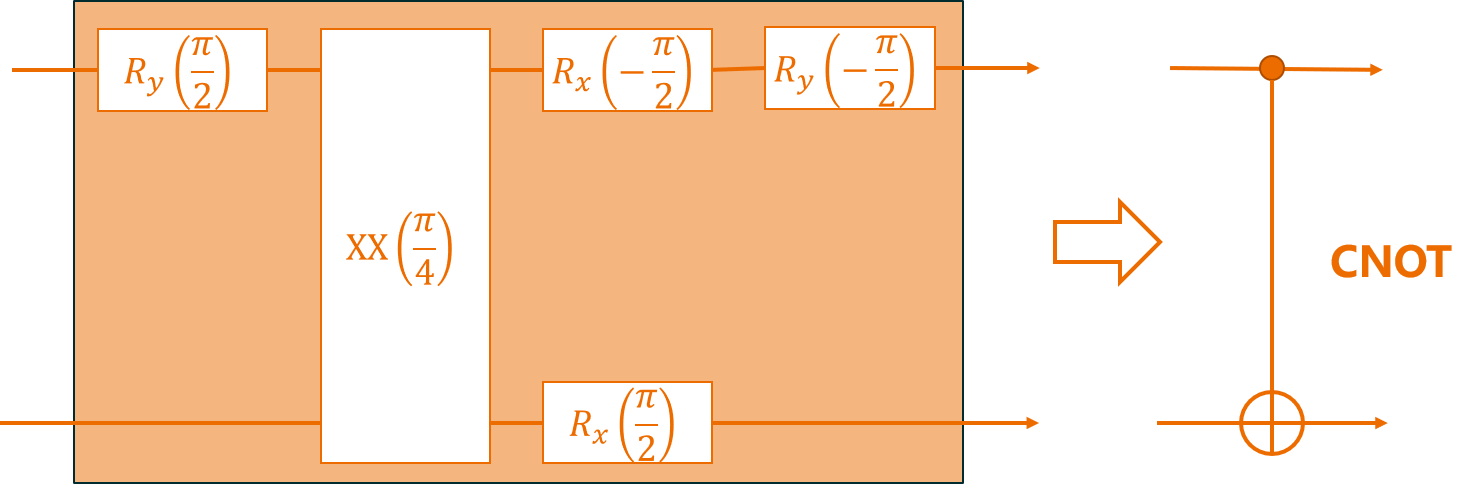
\includegraphics[width=1.0\linewidth]{xx_gate}
\end{figure}

\newpage
\section[章末小结]{章末小结}

相对于传统测控应用领域来说,量子物理实验系统对测控系统时间控制的精度和分辨率、处理器的计算能力、大规模的可拓展性等方面有着更高的要求。为了更好地认识和处理量子物理实验尤其是基于离子阱的量子计算实验系统的需求,本章介绍了面向离子阱量子计算的测控系统研究的重要知识背景。

离子的囚禁是进行离子阱量子计算的基本前提,有了可以在空间中稳定囚禁的离子才能进一步地利用其具备的量子特性进行量子计算的研究。在离子阱量子计算领域中囚禁离子最常使用的是Paul阱,它使用刀片电极生成微波电场对离子进行动态囚禁。本章介绍了此场景下离子的囚禁及其涉及到的经典和量子运动,同时介绍了离子与光场的耦合作为离子比特的态操控的理论基础。此外,对于我们实验室目前所使用的镱离子,系统介绍了它的能级结构、比特编码、激光冷却、量子态的初始化以及态探测等方面的内容,还包括基于微波、连续激光、脉冲激光的离子量子态操控方式和基于离子构建的通用量子门。

通过离子阱量子计算系统这些背景的理解,可以更加深刻地认识到量子系统对测控的实际需求。首先,量子比特操控的操控时间一般在毫秒到微秒级的,其对实时性的要求基本在百微秒至纳秒级,因此要求测控系统应该有微秒或纳秒级的任务时间精确控制能力;而且由于量子的概率特性,一般的实验操作如态的测量往往需要重复几百上千次来获得统计的结果,还有量子纠错等算法的实现需要系统具备实时在线的信息处理和决策能力,这对量子测控系统的实时计算能力有着很强的要求;另外真正实现通用量子计算机至少需要上千个全可控的量子比特,因此大规模的比特控制需要未来的量子测控系统具备强大的可拓展性并且能够用于构建相关系统助力提高量子比特操作的保真度。









% !TeX root = ../sustechthesis-example.tex

\chapter[用于离子阱量子计算的RTMQ测控系统]{用于离子阱量子计算的RTMQ测控系统\label{section:fpga_rtmq}}

% \textcolor{red}{
% 这部分参考RTMQ的相关专利和文档介绍整个测控系统的情况... 
% }

离子量子计算系统的实现涉及到一些物理量的精确调控和测量,这既包括量上的精确性,也包括时间上的精确性。因此系统对测量和控制性能提出了很多新的要求,其中十分关键的一点就是对测控系统实时性的要求。为此我们提出了一套强实时、可拓展、分布式的用于量子物理实验的实时微系统(Real Time Microsystem for Quantum physics, RTMQ),作为离子量子计算的测控系统。在接下来的小节里我将介绍现有实时系统的优缺点以及RTMQ系统的设计架构。随后介绍RTMQ系统的两个重要片上拓展——高速通用数字PID和高速通用数字滤波器的设计实现,以此构建实现离子量子计算的若干重要子系统的数字化推进。

\section[现有实时测控系统]{现有实时测控系统}

% 现有的实时系统一般使用主频在数百MHz至GHz量级的通用微处理器或微控制器作为控制的主体,以计时器中断和时间片分配等方式实现实时控制。这一方案成立的前提在于,所需的时间控制精度与指令执行频率之间有3-6个数量级的差异,因而通用处理器架构中存在的一些诸如分支预判、乱序执行等导致指令执行顺序不确定的因素以及中断系统中存在的现场保护、控制权交接等额外开销导致的时间控制不确定性可以忽略不计。

现有实时系统以通用微处理器或微控制器为主体,通过计时器中断和时间片分配实现实时控制,前提是时间控制精度与指令执行频率差异大,可忽略处理器架构和中断系统的不确定性。然而近来随着量子技术的发展,量子物理实验系统也开始产生对数据处理、复杂流程控制和实时控制的需求。不同于传统行业,量子物理实验系统对时间控制的精度和分辨率的要求在纳秒量级、延迟要求在百纳秒至数十微秒量级,与当前微处理器的主频相当,从而前述的现有的实时控制方案难以满足需求\cite[]{junhua03}。

因此早年在量子物理实验领域内,通常用FPGA(现场可编程门阵列)设计特定的时序脉冲发生器来产生高时间精度的脉冲序列,以此作为其它实验设备的触发信号,进行准确的时序控制。然而,这种方案的灵活性较差,只能产生预定的序列,无法在实验中对实验数据进行即时的处理,或根据实验的中间结果对后续的流程进行及时的调整\cite[]{junhua01}。
% 近年来随着量子算法的发展,实验方案越来越复杂,实验流程中开始包含快速反馈的结构,即在实验过程中对实验目标进行测量,获得一些中间结果,而后对中间结果进行计算和处理,并进而确定后续的实验流程。中间结果的处理和后续流程的确定,一般要求在数十纳秒至数十微秒量级的时间内完成,并且执行时刻必须要严格确定。这要求实验的测控系统具有通用计算的能力,简单的时序脉冲发生器无法满足这一要求。
随着量子算法发展,实验方案复杂,需在数十纳秒至数十微秒内处理中间结果并确定后续流程,简单的时序脉冲发生器已无法满足,实验测控系统需具备通用计算能力。

% 当前领域内针对此问题的主要解决思路为,另置一与时序脉冲发生器紧密连接的通用微处理器,用来对实验数据进行即时处理和产生时序脉冲发生器的后续输出时序。这一方案能较好的满足系统规模较小且实验时序不太复杂的情形下的实时控制需求。然而,这一方案的问题之一在于,微处理器和时序脉冲发生器依然是相互独立的两个个体,而微处理器的执行时序有其内在不确定性;二者之间要保持同步,或者需要频繁地相互交换触发信号,或者需要在时序设计上预留出充足的余量以覆盖此不确定性的最坏情形,总之都会复杂化时序的设计并产生时间浪费。
当前解决问题的思路是另置通用微处理器处理实验数据和产生时序。但该方案存在微处理器和时序脉冲发生器相互独立、同步困难的问题,会复杂化时序设计并产生时间浪费。该方案的另一问题是,系统大时需多个时序脉冲发生器和微处理器,会导致拥塞和同步性问题,而主流微处理器的架构和协议难以实现精确同步。

% 这一方案的另一问题在于,当系统规模较大,一个时序脉冲发生器无法控制整个系统时,就需要同时使用多个时序脉冲发生器,而一个微处理器同时处理过多的实验数据、同时控制过多的时序脉冲发生器,将不可避免的产生拥塞,这会进一步加剧前述的同步性问题。而如果同时使用多个微处理器,则不同微处理器之间的同步性又将成为问题;当前主流的微处理器架构和指令集都是针对通用计算而优化的,主流的微处理器使用的通信协议都是针对高吞吐率而优化的,二者都难以实现精确的时序同步。









% ============================================================================
% ============================================================================
% =======================  RTMQ实时量子测控系统 ===============================
% ============================================================================
% ============================================================================
\section[RTMQ实时量子测控系统]{RTMQ实时量子测控系统}

相对于传统测控应用领域,对于离子阱量子计算研究来说,一种实时性更强、拓展性更好、更灵活的测控系统十分重要。为了满足离子量子计算当前以及未来的测控需求,我们提出了一种实时性拓展性好、具有分布式计算能力的量子测控系统架构——RTMQ(用于量子物理实验的实时微系统,Real Time Microsystem for Quantum physics)。RTMQ系统架构提供了一种新的量子物理实验平台实时测控系统架构,解决了上述的不足。在RTMQ系统架构中,通用计算和时序控制由同一微处理器实现,因此避免了两个独立的模块之间同步性的问题;同时树状结构的系统中每个节点都具有通用计算的能力,因此可以实现计算任务的分布式处理,避免了拥塞的问题\cite[]{junhua01}。



\subsection[RTMQ实时量子测控系统架构]{RTMQ实时量子测控系统架构}

\begin{figure}
    \centering
    \caption[RTMQ实时量子测控系统架构示意图]{RTMQ实时量子测控系统架构示意图\label{fig:rtmq_nodes_and_leaves_structure}}
    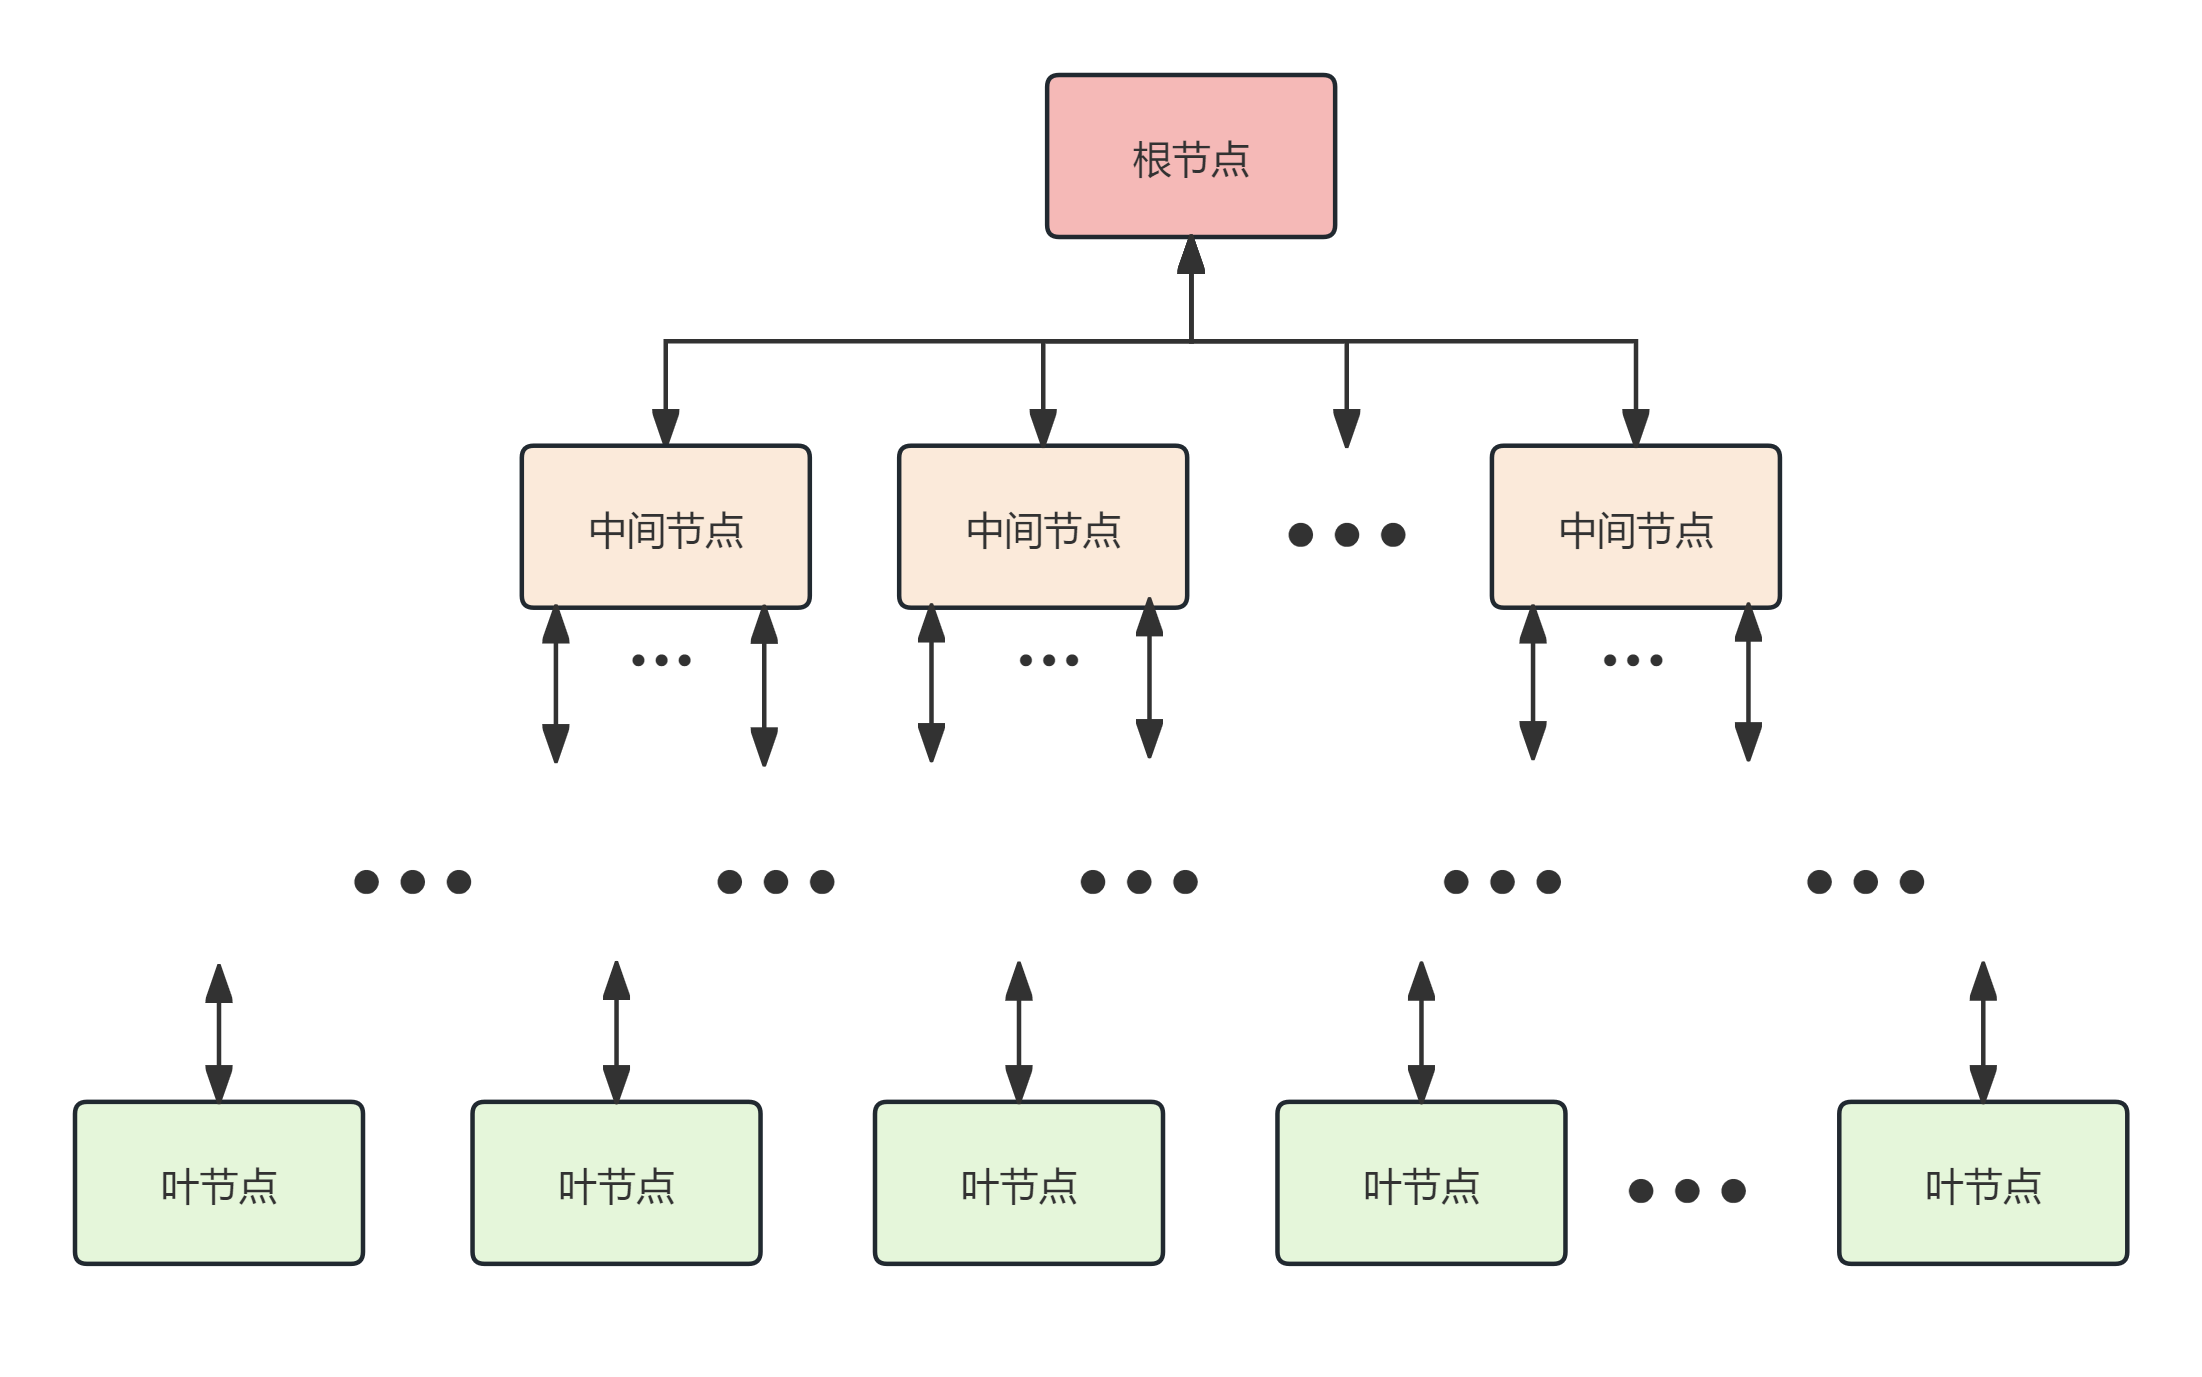
\includegraphics[width=0.6\linewidth]{rtmq/rtmq_nodes_and_leaves_structure}
\end{figure}

RTMQ架构主要用于基于FPGA或ASIC的兼具通用计算和高精度时序控制能力的微系统。系统的整体结构为树状结构,如图\ref{fig:rtmq_nodes_and_leaves_structure}所示,系统包含一个根节点,多个中间结点和多个叶节点;根节点通过网络、USB等方式与控制计算机相连。不同节点可位于同一PCB上,亦可位于不同PCB上。不同节点的时钟通过根节点进行对齐,各个节点都具有独立的控制输出和通用运算能力,能够分布式地完成实验的控制和信息处理。

\begin{figure}
    \centering
    \caption[RTMQ实时量子测控系统架构节点示意图]{RTMQ实时量子测控系统架构节点示意图\label{fig:rtmq_board_overal_structure}}
    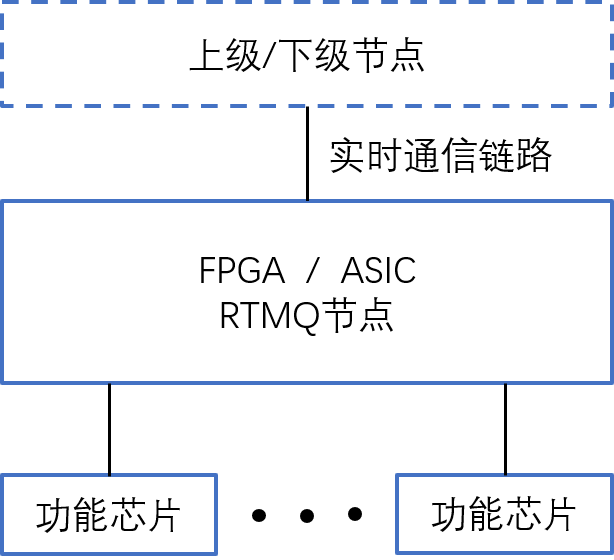
\includegraphics[width=0.4\linewidth]{rtmq/rtmq_board_overal_structure}
\end{figure}

各个节点都由测控硬件板卡构成,一般而言一个板卡具有如图\ref{fig:rtmq_board_overal_structure}所示的结构,板卡上的FPGA或ASIC包含一个RTMQ节点,RTMQ节点通过控制FPGA或ASIC的输入输出与数模/模数转换等各类功能芯片进行交互以实现所需功能,同时通过实时通信链路与其上级和下级节点连接。



\subsection[RTMQ实时量子测控系统架构的节点内部模块]{RTMQ实时量子测控系统架构的节点内部模块}
\begin{figure}
    \centering
    \caption[RTMQ实时量子测控系统架构节点内部模块示意图]{RTMQ实时量子测控系统架构节点内部模块示意图\label{fig:rtmq_board_inner_structure}}
    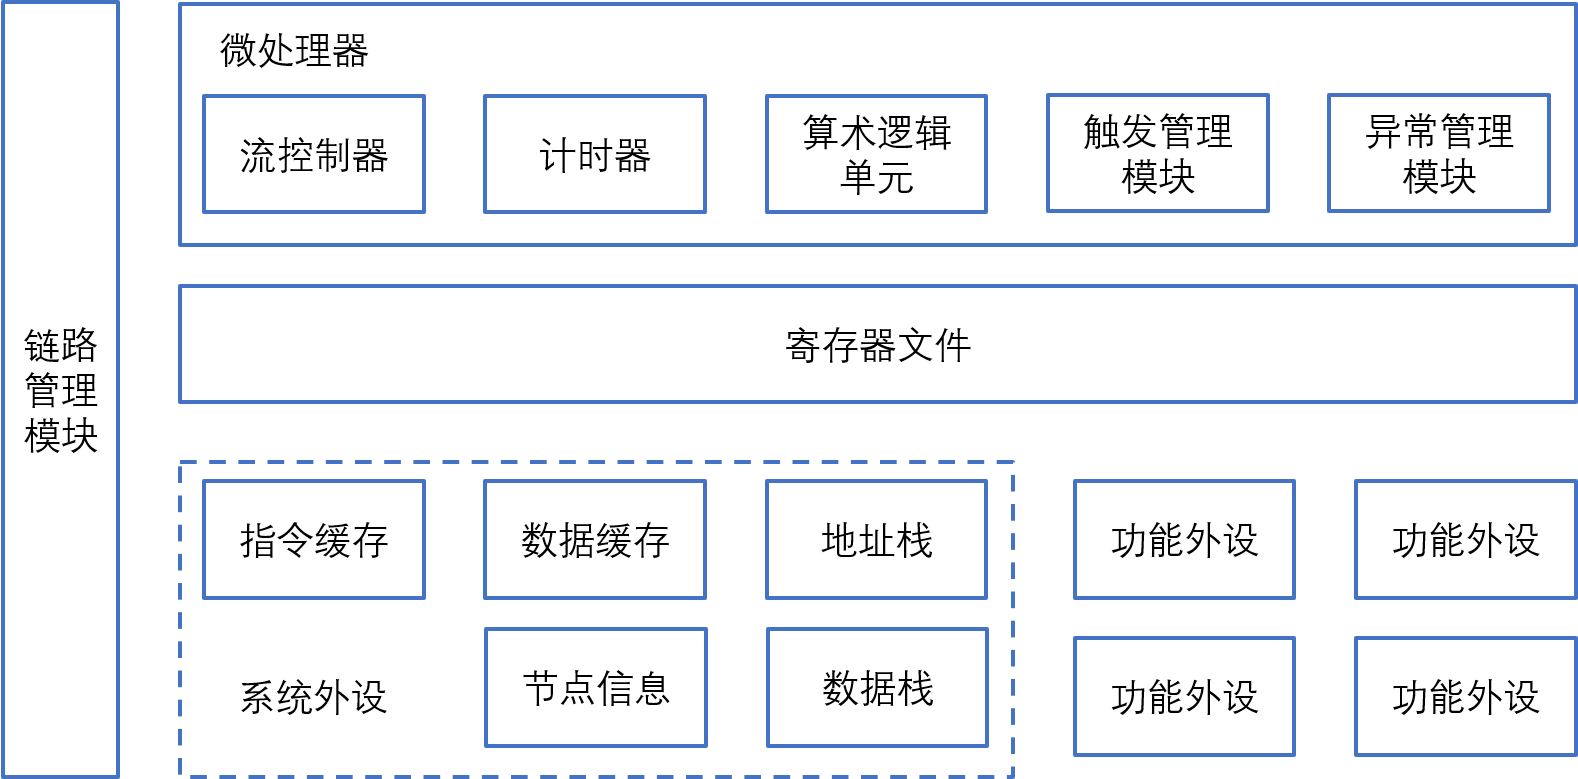
\includegraphics[width=1.0\linewidth]{rtmq/rtmq_board_inner_structure}
\end{figure}

一个RTMQ节点的内部模块如图\ref{fig:rtmq_board_inner_structure}所示,包含一个32位的微处理器、一个寄存器文件、一系列外设模块和一个链路管理模块。其中微处理器包含流控制器、计时器、异常管理模块、触发管理模块和算术逻辑单元5个子模块;寄存器文件包含多个寄存器;外设可分为系统外设和功能外设,系统外设包括指令缓存、数据缓存、节点信息只读存储器以及地址栈和数据栈,功能外设用于实现具体的逻辑或时序功能,可包含多个。

RTMQ架构中包含的微处理器可受指令控制进入挂起状态,而挂起状态可受计时器或触发管理模块的控制恢复正常运行,如此,微处理器的指令流便可以按一定的时间间隔对齐或与外部信号对齐。同时,节点中的系统外设和功能外设的行为受关联寄存器的读写控制,即微处理器的指令与系统各模块的功能和时序有严格的对应关系。因此,本发明提供的架构可实现实时控制与通用计算在指令流层面的结合。
而配置指令插入中断的机制确保了节点对其下级节点的绝对控制,即使下级节点的微处理器处于挂起状态,依然不受影响。配置指令插入中断配合具有确定通信延迟的实时通信链路系统,即可实现时序确定的跨节点的即时反馈控制。

此外,RTMQ架构中每个节点都具有通用计算和时序控制能力,如此,大多数通用计算和时序生成都可以在叶节点或较近的中间结点完成,对于大规模系统不存在拥塞的问题,具有良好的可扩展性。
% \section[测控硬件组成]{测控硬件组成}
% \textcolor{red}{
% 1. 展示实物板卡照片;}
RTMQ测控板实物图如图\ref{fig:rtmq_board_real}所示。RTMQ体系的构成在上述整体硬件核心架构的基础上,还需要结合节点实时通信的链路系统\cite[]{junhua02}来完成节点内部和外部通信的同步,以及相应的实时控制和通用计算的指令集\cite[]{junhua03}来完成对系统的管理和控制。值得关注的是,从它的指令集中可以看到RTMQ测控系统系统是支持板上运算和信息处理的,这是与其它依靠时序发生器构成的测控系统本质不同的地方和优势所在。这些处理包括逻辑运算和算术运算,构成了一个微处理器。而RTMQ系统的微处理器从架构上与CPU有着本质的不同,虽然牺牲了些运算效率,RTMQ的数据处理是严格实时的。这种处理器架构同样也具有拓展性和灵活性,我们可以方便地为它拓展和定义多种运算方式,也可以为其添加外设模块等,以适应更多更复杂任务的需求。在下面几小节中,我将介绍一些基本运算及外设模块的实现和使用。

\begin{figure}
    \centering
    \caption[RTMQ测控板去壳单板实物图]{RTMQ测控板去壳单板实物图\label{fig:rtmq_board_real}}
    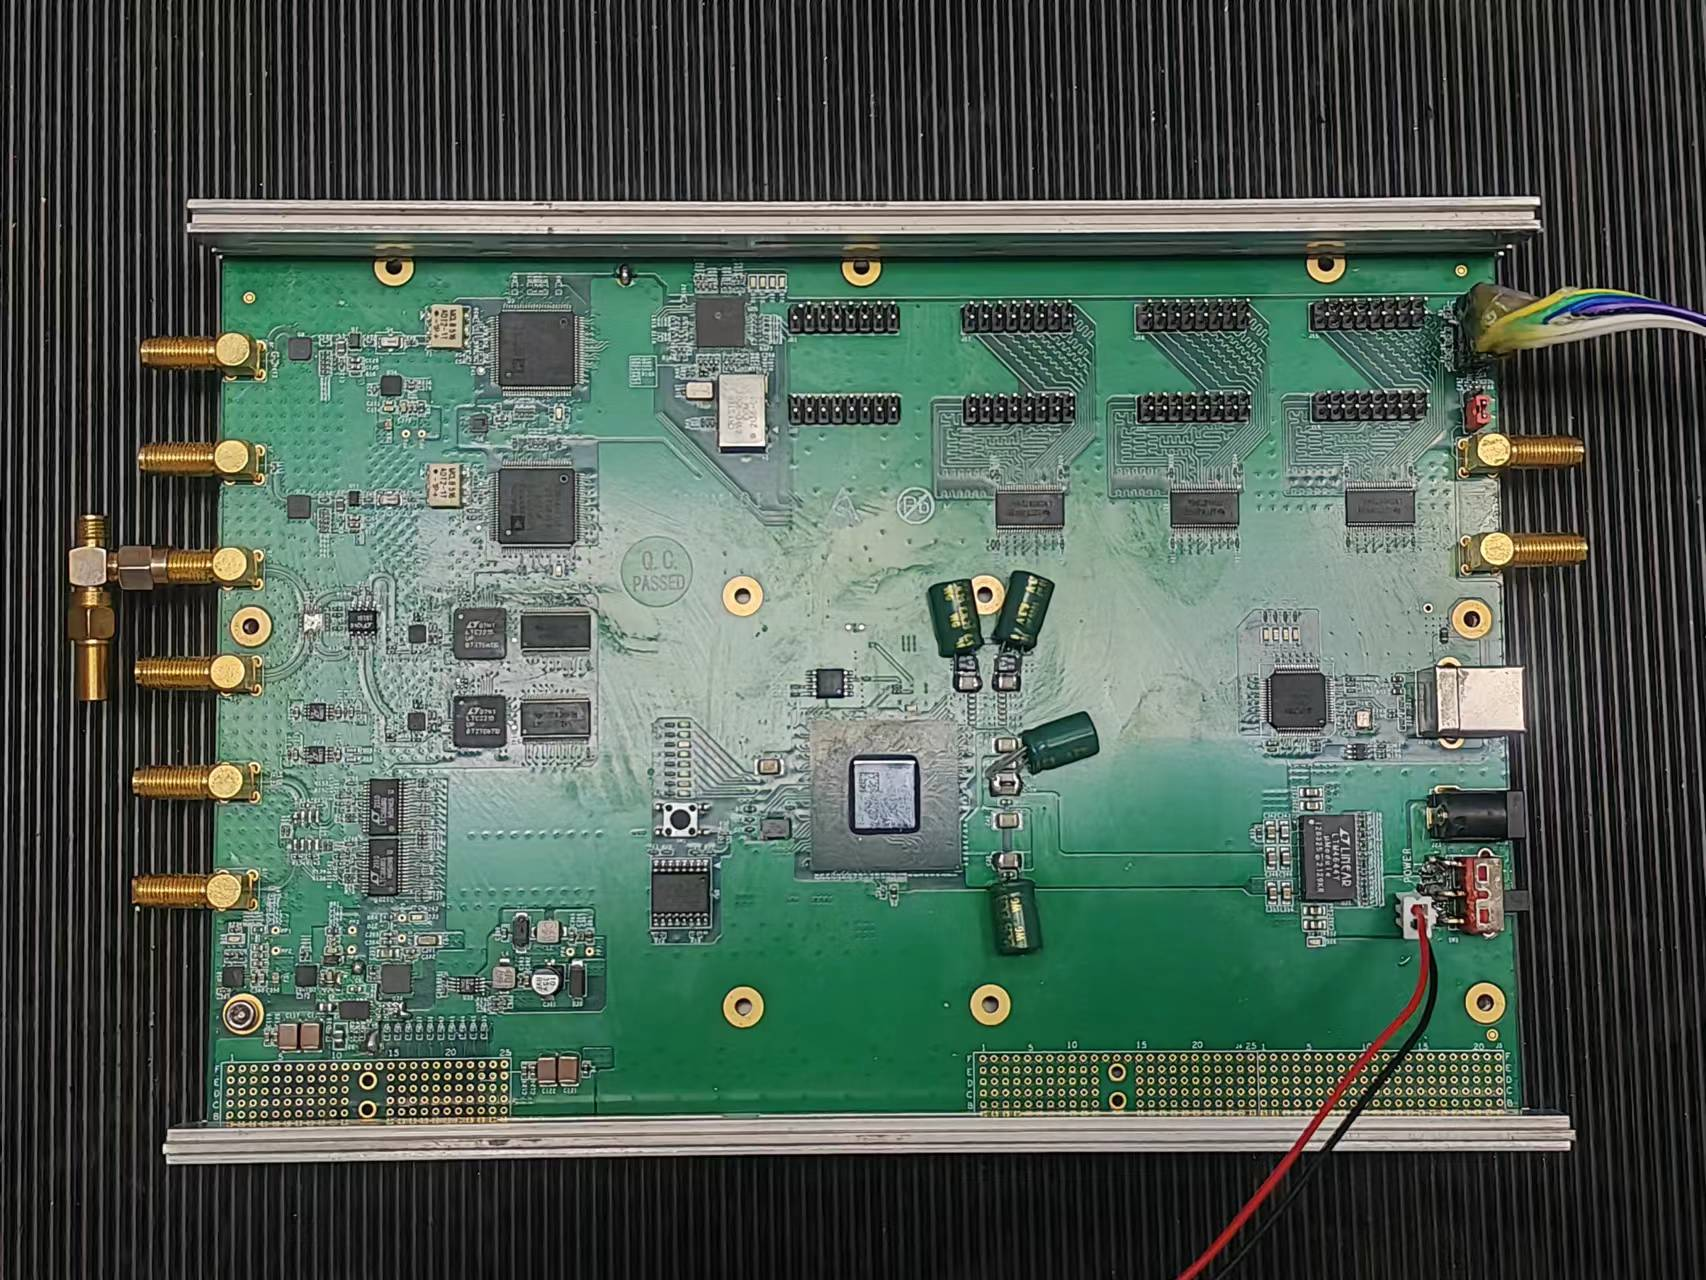
\includegraphics[width=1.0\linewidth]{rtmq/rtmq_board_real}
\end{figure}



% ============================================================================
% ============================================================================
% =======================      高速数字PID      ===============================
% ============================================================================
% ============================================================================

\section[基于FPGA的高速通用数字PID]{基于FPGA的高速通用数字PID\label{section:digital_pid}}
% \textcolor{red}{
% 1. 介绍数字PID功能、逻辑图、Vivado中的实现、优势;}
当前量子计算系统中大量采用PID控制器进行诸如激光功率稳定、激光相位稳定、激光拍频锁定等等控制系统的构建,常用的器件有如LB1005模拟伺服控制器。这类模拟控制器的确定在于稳定性较差且价格昂贵,此外它的集成度也比较差,往往需要占用较大的实验平台面积。除此之外这类模拟PID控制器往往采用机械旋钮进行参数调节,不利于进行实验系统的集成化和自动化。与之相比较,使用融合了高速通用数字PID的RTMQ测控系统可以同时完成对实验序列的操控和对设备关键参数的伺服控制。除此之外,采用也对系统完成了集成化和数字化,提高了系统的稳定性和易用性。

\subsection[数字PID]{数字PID}
数字PID控制器是一种常用的自动控制算法,用于实现对系统的闭环控制。PID控制器通过对系统的误差进行比例(Proportional)、积分(Integral)和微分(Derivative)计算,生成控制信号来调整系统的输出,以达到期望的控制效果。在量子测控系统中很多地方都需要用到闭环控制,比如激光的功率稳定、激光的波长稳定、离子阱频率稳定等。相对于模拟PID控制器,数字PID控制器具有结构简单、易于实现、控制灵活、工作稳定等优点,是RTMQ系统中的重要组成部分。

PID 控制器的数学表达式可以表示为:
\begin{align}
    u(t)= K_p e(t) + K_i \int_{0}^{t} e(\tau) d\tau + K_d \frac{d e(t)}{dt}
\end{align}

其中,$u(t)$是控制器的输出,$e(t)$是系统的误差,$K_p$、$K_i$和$K_d$分别是比例系数、积分系数和微分系数。
 
PID控制器的实现可以分为模拟PID和数字PID两种方式。模拟PID是通过模拟电路实现的,而数字PID是通过数字计算实现的。数字PID控制器通常使用微处理器或计算机来实现,其基本结构包括采样、计算和输出三个部分。数字 PID 控制器的实现步骤如下:
\begin{itemize}
    \item 采样:对系统的输入和输出进行采样,获取当前时刻的误差值e(t);
    \item 计算:根据采样得到的误差值,按照 PID 控制器的数学表达式计算控制信号u(t);
    \item 输出:将计算得到的控制信号输出到执行机构,调整系统的输出;
\end{itemize}

在数字PID控制器的实现中,需要对积分和微分操作进行离散化处理。常用的离散化方法有矩形法和梯形法。矩形法将积分区间划分为若干个相等的子区间,每个子区间的积分值近似为矩形的面积;梯形法将积分区间划分为若干个相等的子区间,每个子区间的积分值近似为梯形的面积。这一步骤在嵌入式系统中通常使用模拟数字转换(ADC)芯片来完成。

\subsection[数字PID的增量表达式]{数字PID的增量表达式}
硬件资源在FPGA中是十分宝贵的资源,而乘法器这样的器件往往会占用大量的硬件资源。因此在满足时序要求的情况下我们希望能够尽量减少乘法器的使用,PID的增量表达式就是一种可以有效减少PID硬件电路实现过程中乘法器需求个数的方式,下面将介绍这种方法。

\begin{figure}
    \centering
    \caption[数字PID结构示意图]{数字PID结构示意图。MULT:乘法器;Reg:寄存器;ADD:加法器;SUB:减法器;$y_t, u_t$:输入和输出信号;$ref$:参考值输入;$k_0, k_1, k_2$:增量表达下的PID控制参数。\label{fig:digital_pid_structure_16bits_s}}
    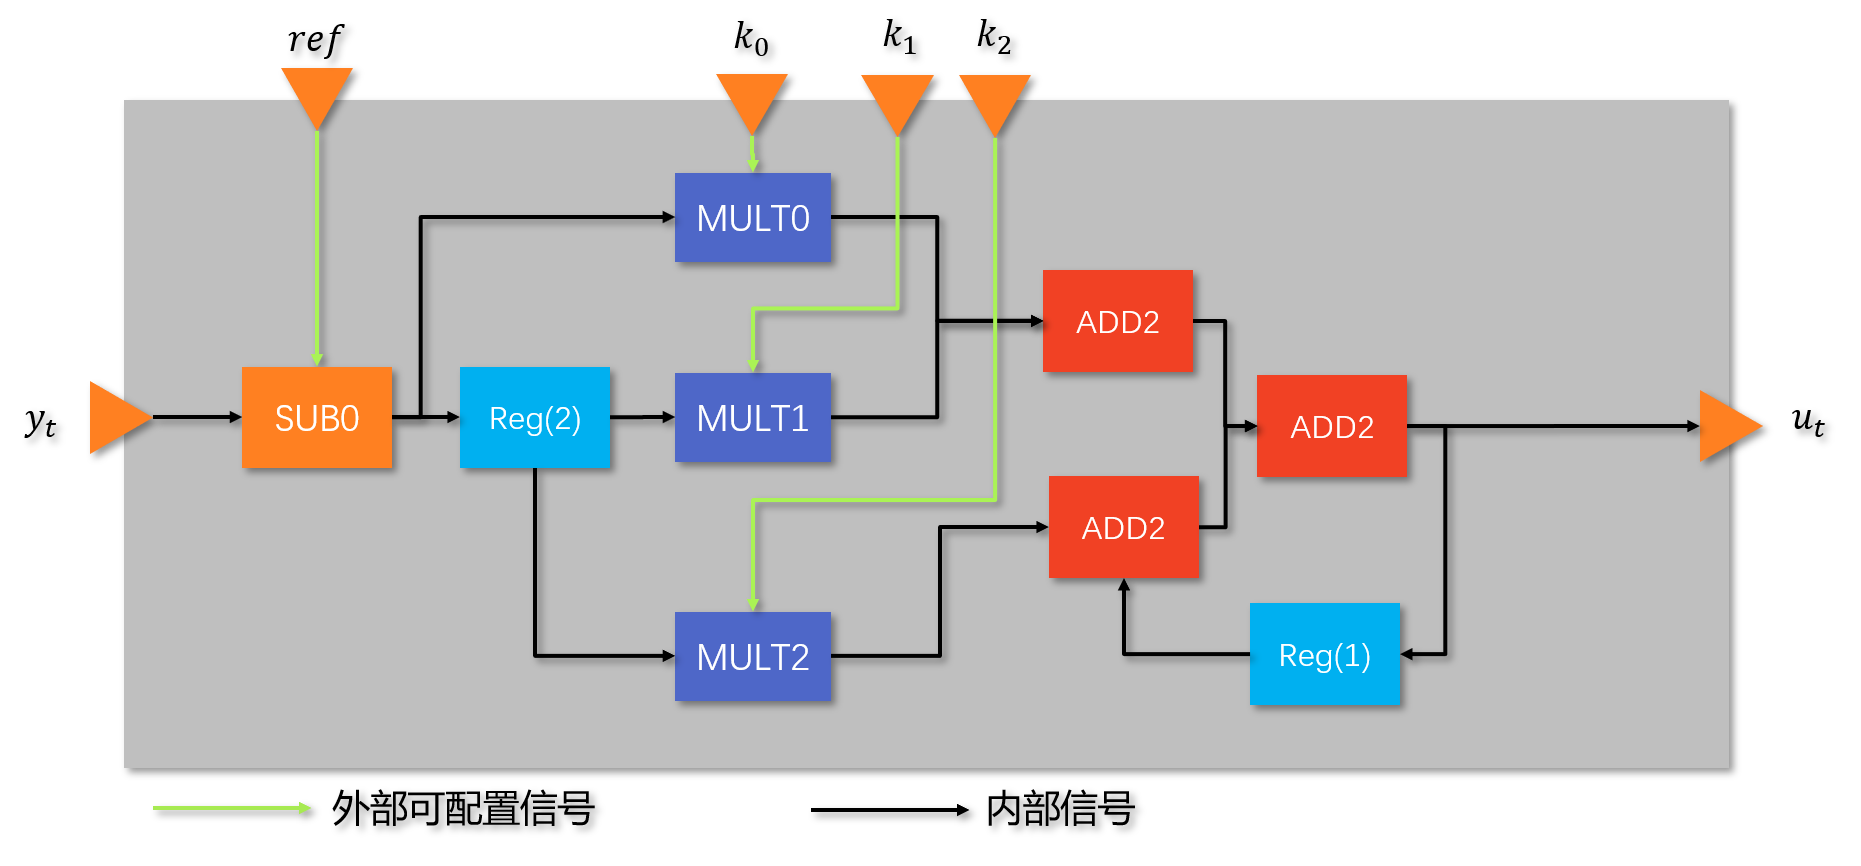
\includegraphics[width=1.0\linewidth]{rtmq/digital_pid_structure_16bits_s}
\end{figure}

离散化后的PID表达式为:
\begin{align}
    u(n)=k_p e(n)+k_i\sum_{j=-}^{n}e(j)+k_d[e(n)-e(n-1)]\\
    u(n-1)=k_p e(n-1)+k_i \sum_{j=0}^{n-1}e(j)+k_d [e(n-1)-e(n-2)]
\end{align}

由上面两式可以导出:

\begin{align}
    \Delta u(n)=&u(n)-u(n-1)\\
    =&k_0 e(n)+k_1 e(n-1)+k_2 e(n-2)
\end{align}

其中$k_0=k_p+k_i+k_d,\ k_1=-k_p-2k_d,\ k_2=k_d$,这个式子被称为PID的增量算法。采用这种形式的好处是避免了计算PID原始表达式中的无限积分项。在这种增量式的方式下,PID的控制输出可以表达为:
\begin{align}
    u(n)=u(n-1)+\Delta u(n)=u(n-1)+k_0 e(n)+k_1 e(n-1)+k_2 e(n-2)\label{eq:increment_pid}
\end{align}

按照上述式\eqref{eq:increment_pid}表示的增量式算法,数字PID实现的结构示意图如图\ref{fig:digital_pid_structure_16bits_s}所示。接口主要有参考$ref$、参数$k_0, k_1, k_2$等可配置输入,反馈信号$y_t$等系统回路输入,以及$u_t$等系统控制输出。用到的器件包括加法器/减法器(图示中红、橙色模块)、乘法器(图示中蓝色模块)、寄存器(图示中靛色模块)。

\subsection[高速通用数字PID的FPGA实现]{高速通用数字PID的FPGA实现}

% 增量式PID最终在FPGA中实现的结构图如图\ref{fig:digital_pid_structure_16bits}所示。

根据图\ref{fig:digital_pid_structure_16bits_s}所示的结构,可以在FPGA中实现硬件的PID。其中主要涉及到的数字加法器、数字乘法器,分别采用的是超前进位加法器和Booth乘法器。对于高速时序电路,尤其是要满足与RTMQ的实时性匹配等相关需求,在开发过程中需要注意流水线的设置和对齐,最终的实现硬件框图如图\ref{fig:digital_pid_structure_16bits}所示,其硬件输出测试和仿真对比如\ref{fig:pid_compare}图所示。从图\ref{fig:pid_compare}中可见,在Vivado中实现的高速PID硬件电路在$k_i=1, k_d=1$的情况下经过大概1000ns后即可以将系统的输出稳定在参考值1000附近,与直接使用MATLAB进行数字PID仿真输出结果一致。

\begin{figure}
    \centering
    \caption[16位数字PID的FPGA实现结构图]{16位数字PID的FPGA实现结构图上\label{fig:digital_pid_structure_16bits}}
    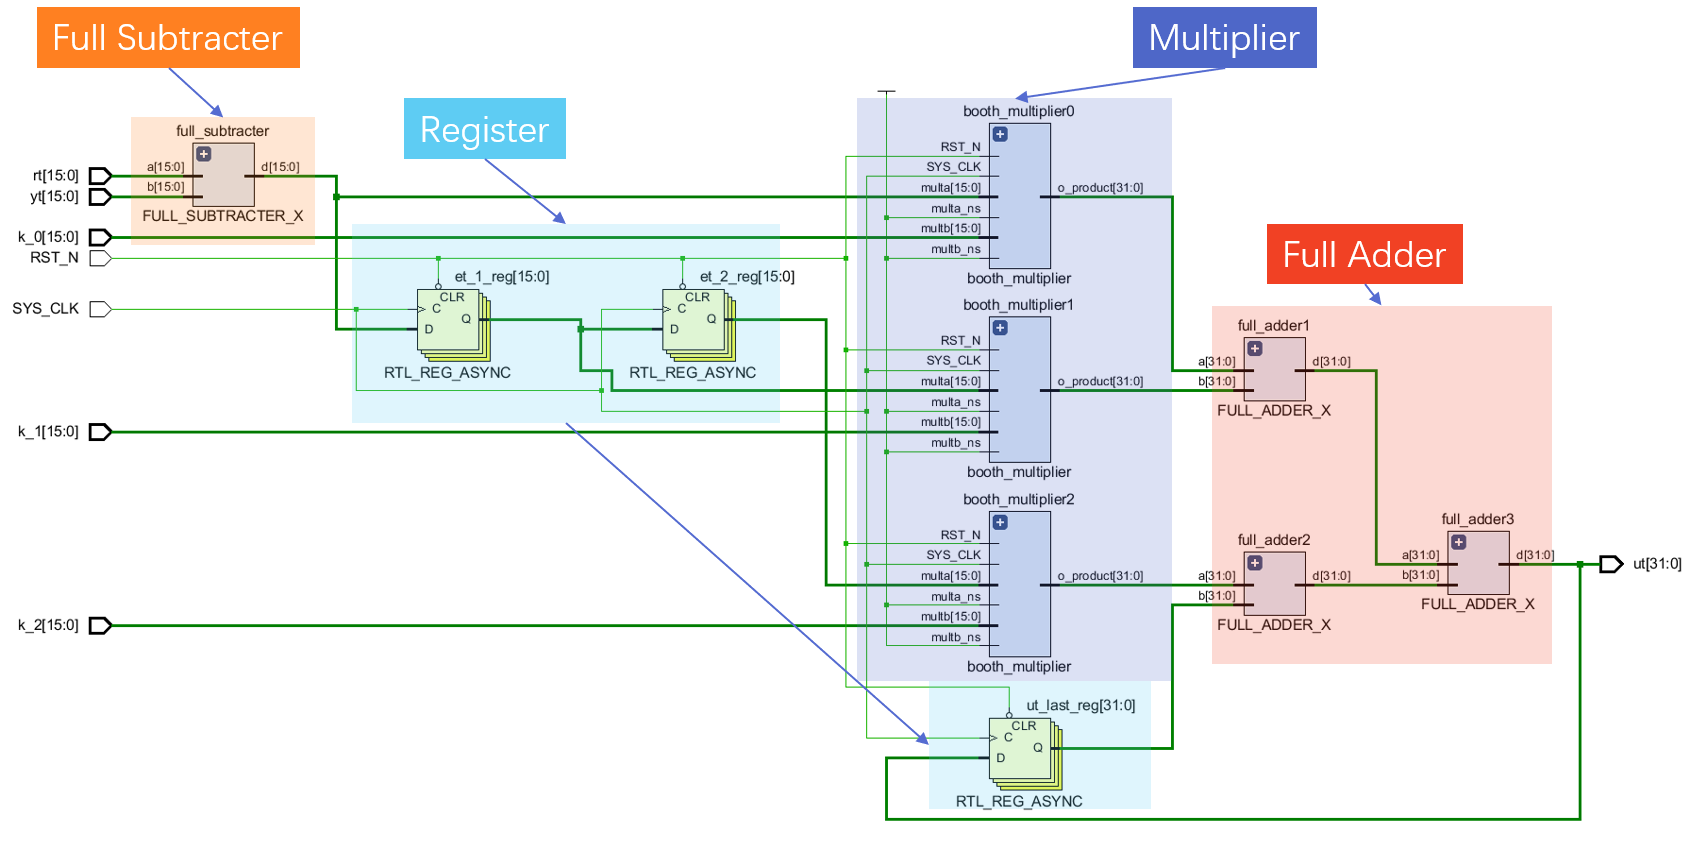
\includegraphics[width=1.0\linewidth]{rtmq/digital_pid_structure_16bits}
\end{figure}

\begin{figure}
    \centering
    \caption[16位数字PID的FPGA实现结果与仿真结果对比]{16位数字PID的FPGA实现结果与仿真结果对比。初始系统输出和调节输出都为0,参考数值为1000,$k_i=1, k_d=1$,Vivado综合输出时长为3500ns,仿真持续时间为1000$T_c$(系统仿真迭代次数)。\label{fig:pid_compare}}
    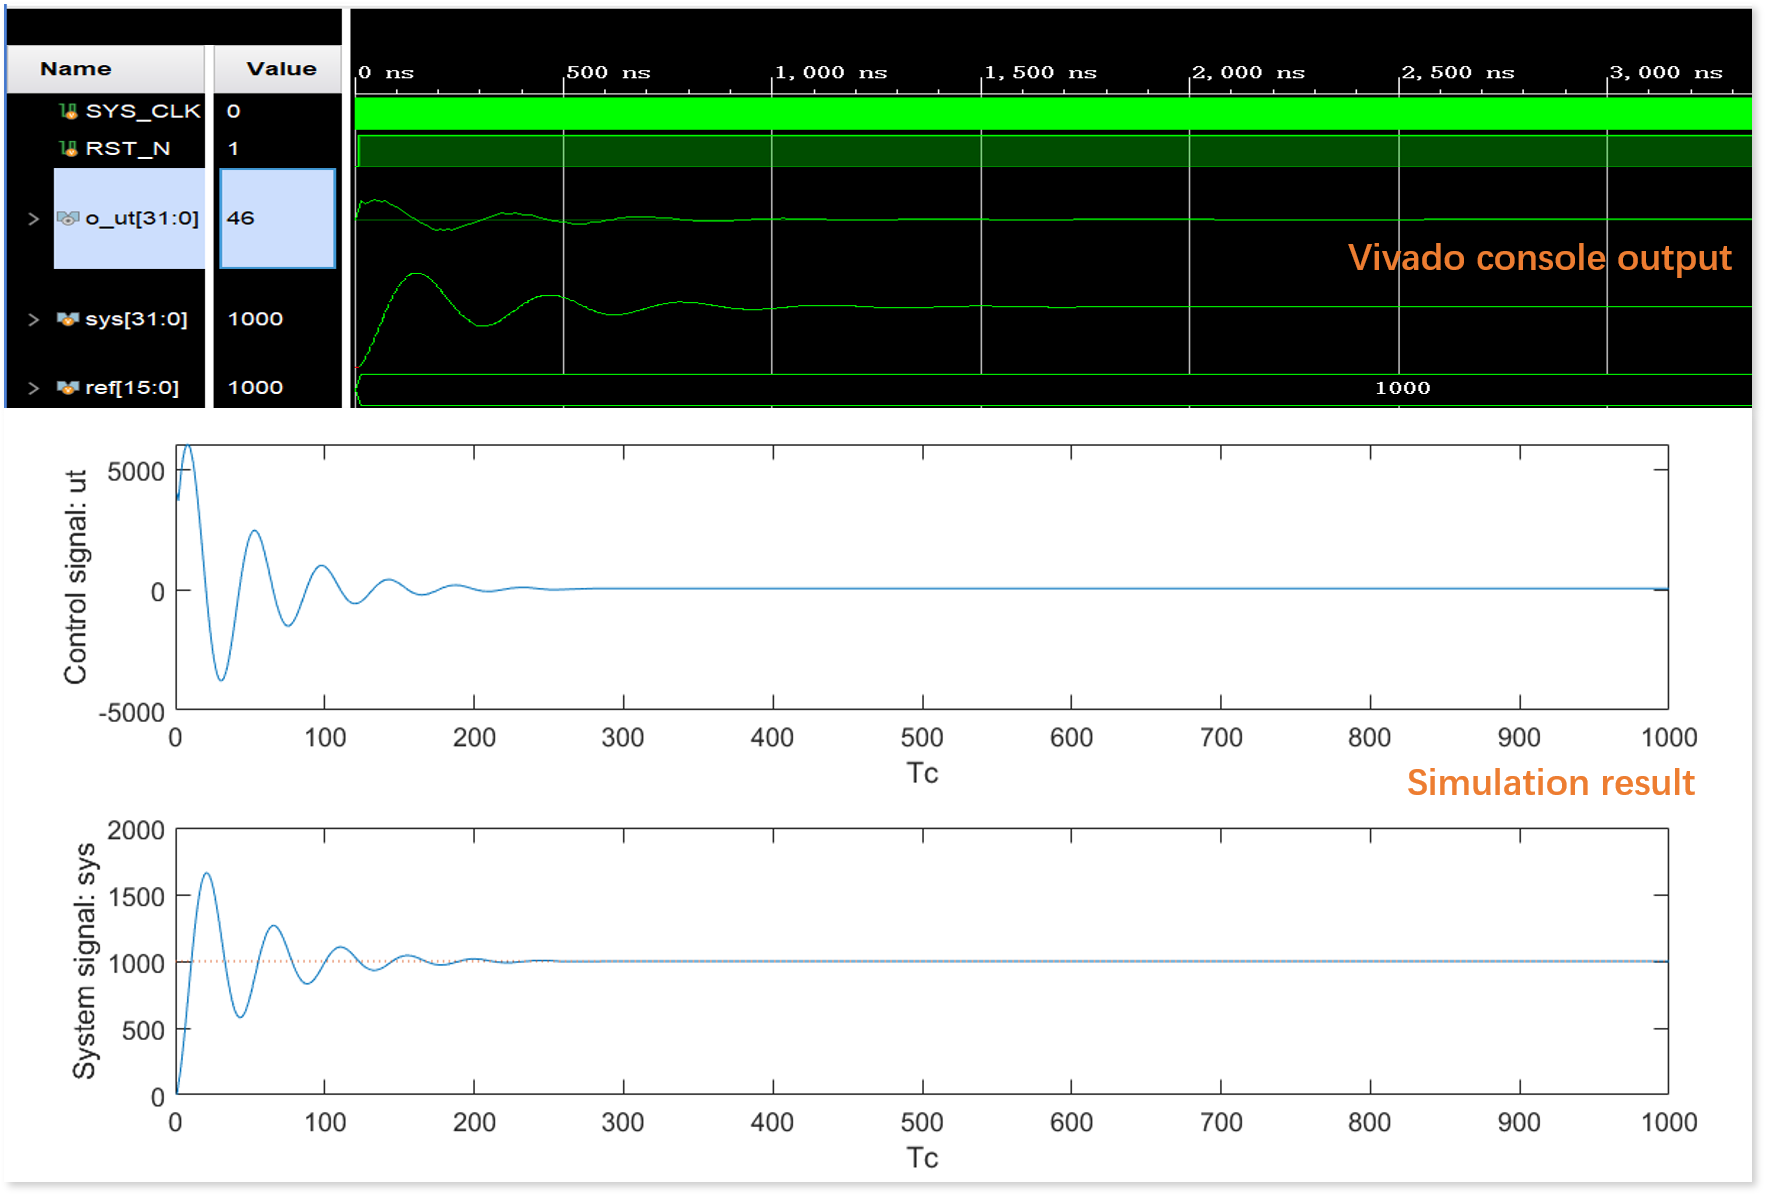
\includegraphics[width=1.0\linewidth]{rtmq/pid_compare}
\end{figure}

整个PID控制器使用了一个减法器、三个加法器、三个乘法器和若干寄存器。图\ref{fig:digital_pid_structure_16bits}是一个16位输入的数字PID,它的输出是32位的,该实例模块总共包含9级流水线,工作频率可达200MHz以上。对更低或者更高位数的数字PID控制器,可以通过替换相应位数的加减运算和乘法模块,并调整相应的寄存器位宽来方便地得到。







% ============================================================================
% ============================================================================
% =======================     高速数字滤波器    ===============================
% ============================================================================
% ============================================================================
\section[基于FPGA的高速通用数字滤波器]{基于FPGA的高速通用数字滤波器\label{section:digital_iir}}

在量子计算的实现过程中,对于噪声的抗争从未停止。而对抗噪声的一种十分有效的方式就是使用各种各样的滤波器来对信号进行过滤以提高有用信号的质量。本质来讲,滤波器是一种选频装置,可以使信号中特定的频率成分通过,而极大地衰减其它频率成分。利用滤波器的这种选频作用,可以滤除干扰噪声或进行频谱分析。
当前实验系统中广泛出现滤波器为模拟滤波器,但是随着量子测控系统的数字化集成化进行逐步加深,在很多内部信号的处理上也有相当多的滤波需求,比如消除ADC芯片采样的噪声等。我们特别地在RTMQ系统板卡上实现了相匹配的高速通用数字滤波器,来进一步实现对量子物理实验系统信号的控制和优化。


% \subsection[数字滤波器]{数字滤波器}
% \textcolor{red}{
% 1. 介绍数字滤波器功能、种类、基本原理,比如有限冲激响应滤波器、无限冲激响应滤波器等等;}


\subsection[无限冲激响应滤波器IIR]{无限冲激响应滤波器IIR}
数字滤波器的基本原理是利用离散系统的特性对输入信号进行加工和处理,改变输入信号的频率特性,从而达到选频、提高信噪比、消除干扰等目的。数字滤波器一般由延迟单元、加法器、乘法器、寄存器等基本运算单元组成。不同类型的数字滤波器有不同的实现方法和应用领域。在通信、语音处理、图像处理、信号处理等领域,数字滤波器都有着广泛的应用。整个离子阱系统中很多模块都有滤波器的需求以获取更高质量的信号来控制量子比特。为此,整个RTMQ系统中需要实现数字滤波器以供系统设计和实现使用。

有限冲击响应滤波器(FIR滤波器)的冲激响应在有限时间内衰减为零,其输出仅取决于当前和过去的输入信号值。FIR滤波器在保证幅度特性的同时,很容易做到严格的线性相位特性。无限冲击响应滤波器(IIR滤波器)的冲激响应理论上应会无限持续,其输出不仅取决于当前和过去的输入信号值,也取决于过去的信号输出值。

有限冲击响应滤波器(FIR滤波器)的优点是具有线性相位、稳定性好、容易实现等,缺点是阶数较高时,运算量较大,对存储空间要求较高。无限冲击响应滤波器(IIR滤波器)的优点是阶数较低时,运算量较小,对存储空间要求较低,缺点是相位非线性、稳定性较差、设计复杂等。实际滤波器设计经验表明,实现相同形状的滤波效果,IIR滤波器所需的计算资源远小于FIR滤波器。鉴于硬件实现是对资源十分敏感的,因此我们选用IIR滤波器来进行实现。

IIR滤波器的冲激响应理论上应会无限持续,其输出不仅取决于当前和过去的输入信号值,也取决于过去的信号输出值,用差分方程来表示一个滤波器,其表达式为:
\begin{align}
    y(n)=\sum_{k=1}^Na_ky(n-k)+\sum_{k=0}^Nb_kx(n-k)\label{eq:iir_filter}
\end{align}

 % \textcolor{red}{
% 2. 介绍数字通用滤波器功能、逻辑图、Vivado中的实现、优势;}

其中,$y(n)$表示输出信号,$x(n)$表示输入信号,$a_k$和$b_k$表示滤波器系数。本质上来说,IIR滤波器就是将输入和过去的输出按照某种方式加权计算获得最终输出结果的。对于一个给定阶数和数字位数的IIR滤波器,它的形状完全取决于系数$a_k$和$b_k$。因此,为了维持通用性,在硬件实现的过程中,我们应该把系数($a_k, b_k$)设计为可外部软件配置的。
以四阶为例,通用四阶IIR滤波器的结构框图如图\ref{fig:iir_filter_s}所示,图中$a_0-a_3, b_0-b_3$为IIR滤波器的可配置系数,主要用到的模块有寄存器、乘法器、加法器等。
\begin{figure}
    \centering
    \caption[IIR滤波器结构框图]{IIR滤波器结构框图\label{fig:iir_filter_s}}
    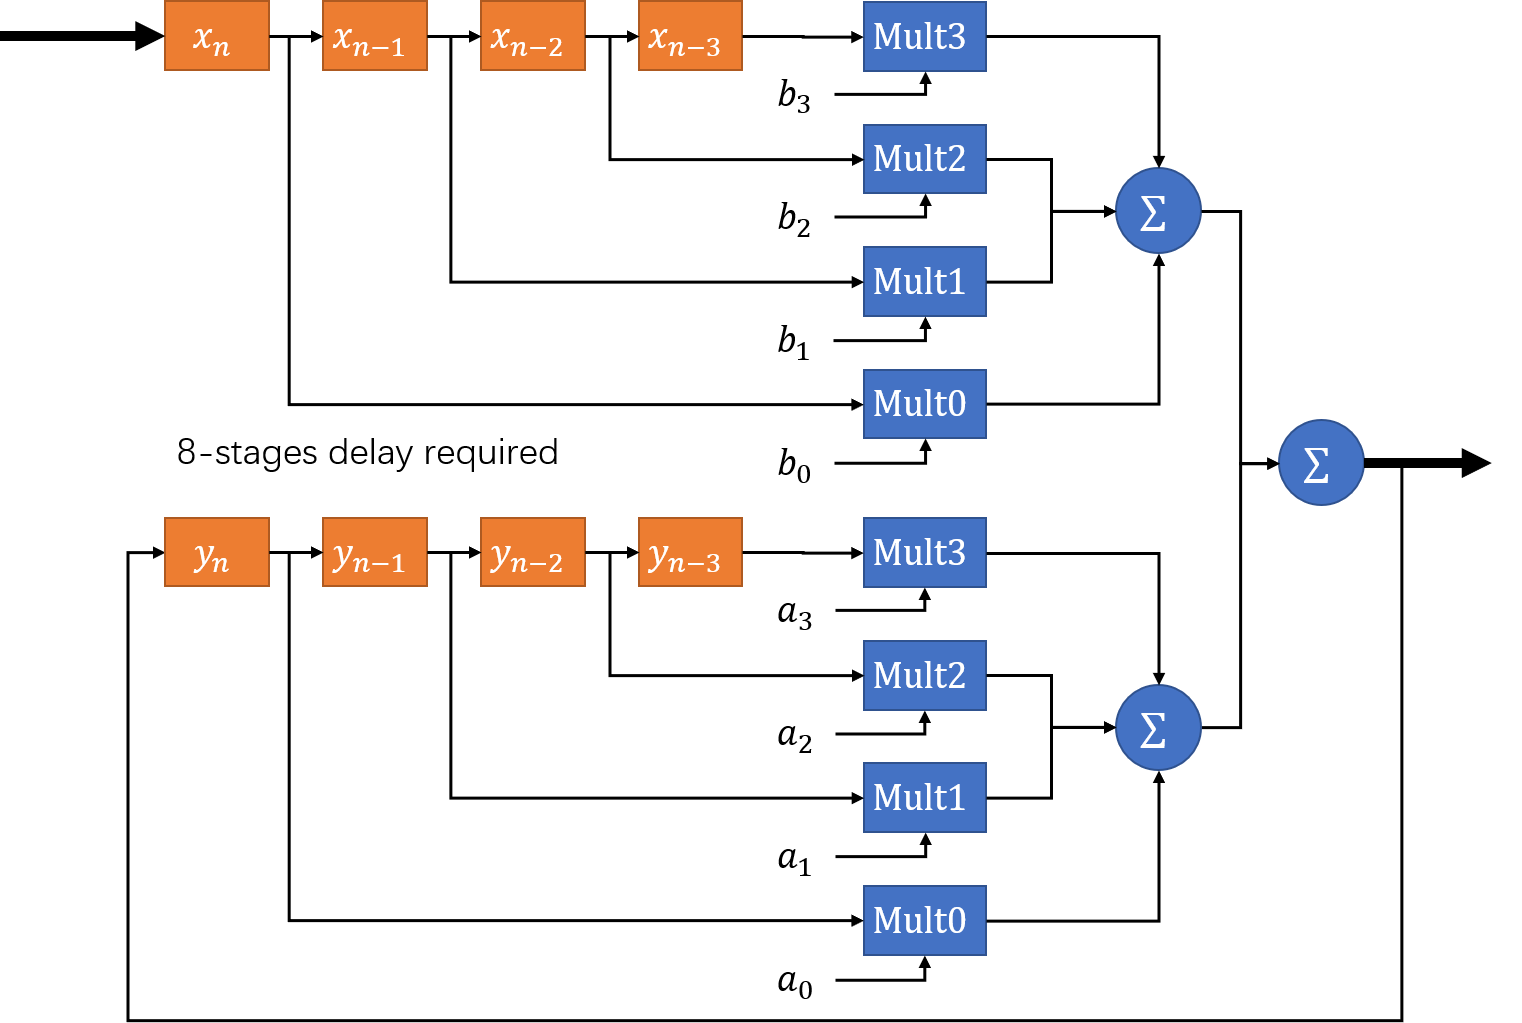
\includegraphics[width=1.0\linewidth]{rtmq/iir_filter_s}
\end{figure}


\subsection[高速通用数字IIR滤波器的FPGA实现]{数字IIR滤波器的FPGA实现}

根据图\ref{fig:iir_filter_s}给出的结构图和公式\eqref{eq:iir_filter},可以将其在FPGA中进行实现和验证。数字IIR滤波器在FPGA中的实现结果的结构图如图\ref{fig:iir_filter_vivado}所示,整体结构中超如了若干的流水线用于对齐$x(n)$和$y(n)$的时序。除此之外,流水线也被用于满足电路的时延要求。需要注意的是,由于上一时刻的输出结果$y(n-1)$需要参与到下一时刻的输出结果的计算中,因此从计算结果到迭代反馈之间仅能有一级流水线存在,否则输出结果就会出错。也即从乘法器输入到乘法器输出,以及加法器输入到加法器输出并反馈到乘法器输入这个回路中只能存在一级流水线。正因此,这个IIR滤波器无法工作在较高的频率上,需要在板上额外配置工作频率,该32位通用IIR滤波器设计在FPGA板上的工作频率为25MHz。

\begin{figure}
    \centering
    \caption[IIR滤波器实现结果的结构图]{IIR滤波器实现结果的结构图(Vivado)\label{fig:iir_filter_vivado}}
    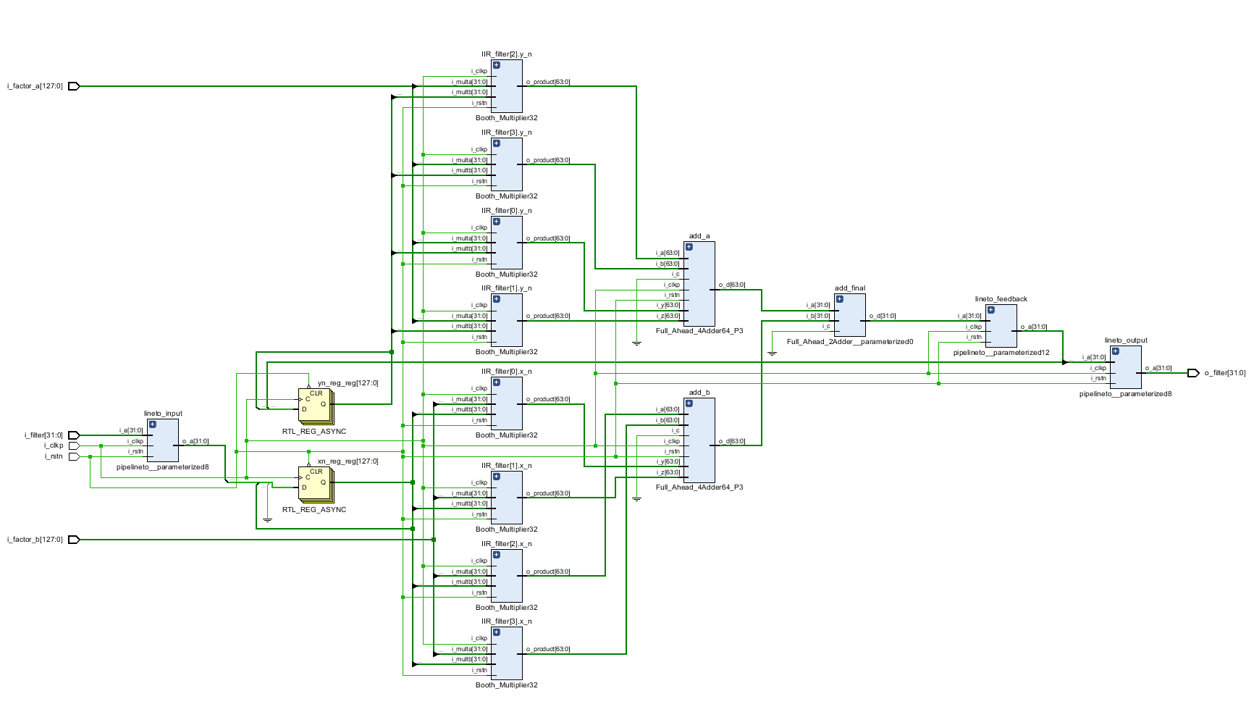
\includegraphics[width=1.0\linewidth]{rtmq/iir_filter_vivado}
\end{figure}




\subsection[滤波器形状测量]{滤波器形状测量}
数字滤波器的形状设计可以采用MATLAB中的滤波器设计器来完成。在量子计算的试验系统中常常要应对的是高频信号噪声,低通滤波器是十分常见的需求,因此下面以低通滤波器为例进行说明。如图\ref{fig:filter_design_real1},通过MATLAB设计了一个截止频率在100kHz附近的巴特沃斯型迭代滤波器,结果为一个3阶的迭代滤波器,参数为:$a_0=16777216;
a_1=-33470572;
a_2=16693565;
a_3=0;
b_0=52;
b_1=105;
b_2=52;
b_3=0$。可以看到设计的理论截止频率(100kHz)和数字滤波器实际的截止频率(13.17kHz)有较大的差异。其原因主要有两方面:1. 数字滤波器的设计本身实际上是对模拟滤波器的近似,因而结果不绝对准确;2. 实际在FPGA中的硬件滤波器运算位宽有限,爹地啊过程中存在截断效应;3. 对数据的表征不够精确,测试的过程中用到模数转换(16位)等中间数字过程。

\begin{figure}
    \centering
    \caption[IIR滤波器设计仿真和实际测试结果]{IIR滤波器设计仿真和实际测试结果\label{fig:filter_design_real1}}
    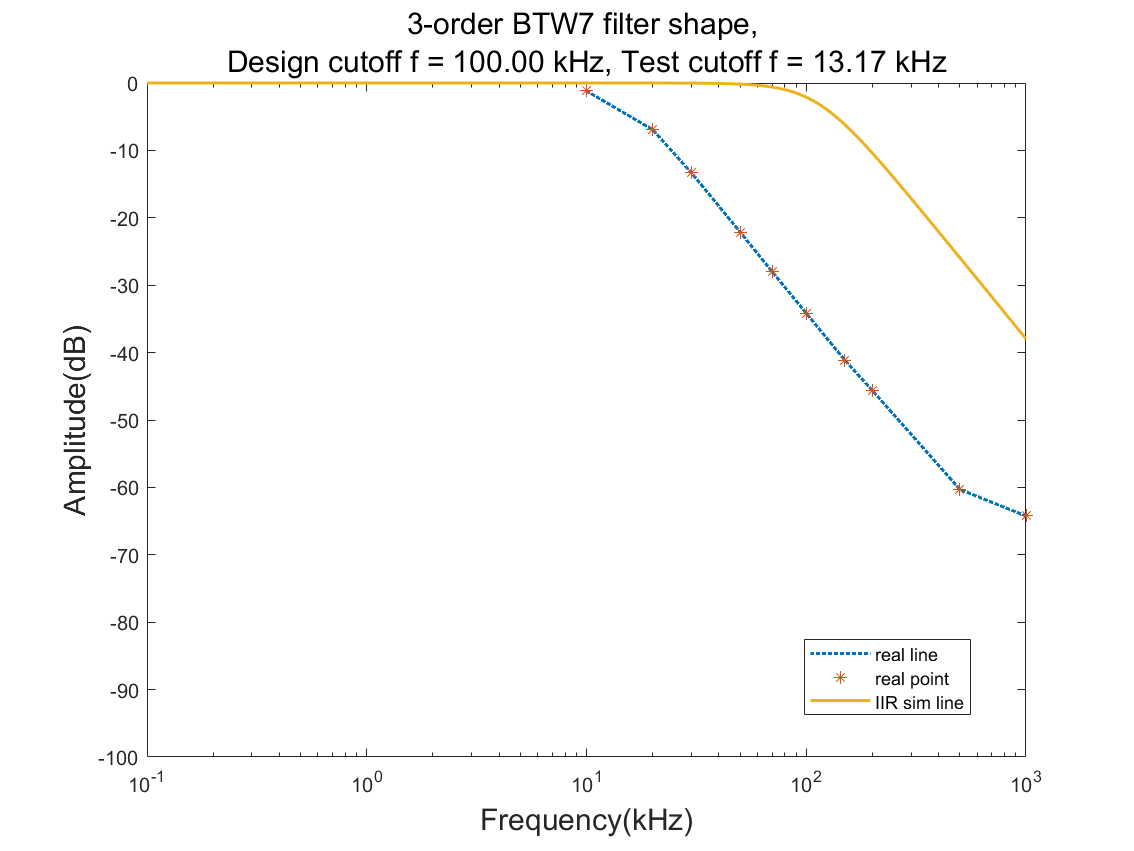
\includegraphics[width=1.0\linewidth]{rtmq/filter_design_real1}
\end{figure}

在理论结果绘制中,对滤波器的结果进行类似FPGA硬件中的人工截断,得到的模拟结果如图\ref{fig:filter_design_real2}所示。可以看到此时理论设计的截止频率结果与实际硬件数字PID的截止频率结果变得更加接近了。尽管仍然存在一定的差异,已经可以给出比较有意义的指导信息了。整体上来看,硬件实现的数字滤波器在配置为低通滤波器的时候带宽会被压窄。因此如果需要100kHz的带宽,则需要在设计时适当放大这个带宽需求。最终实际的滤波器带宽可以通过测量来进一步验证是否符合使用要求,如果不符合则可以重新设计和测试。值得一提的是,在实现了通用的硬件IIR滤波的基础上,重新设计和配置$a_0-a_3, b_0-b_3$等参数是十分方便快捷的,仅需更改可配置寄存器的值即可。

\begin{figure}
    \centering
    \caption[IIR滤波器考虑截断的仿真和实际测试结果]{IIR滤波器考虑截断的仿真和实际测试结果\label{fig:filter_design_real2}}
    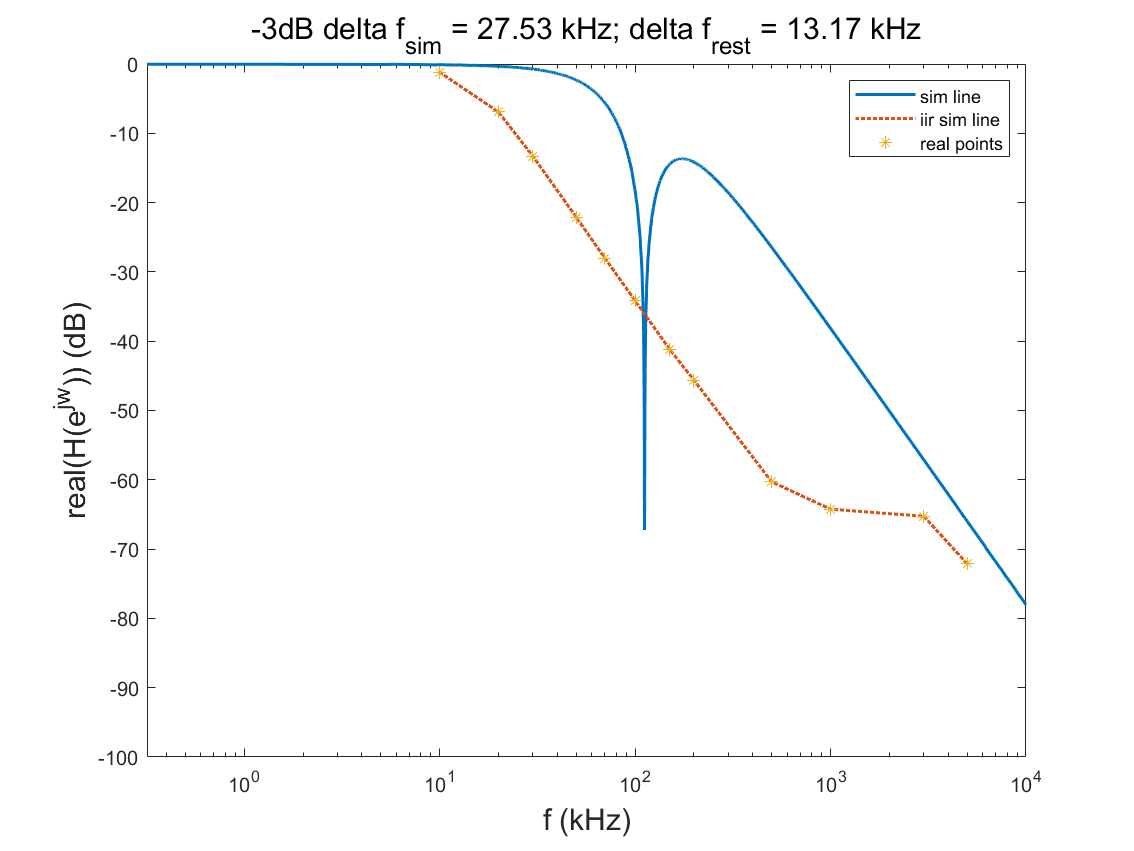
\includegraphics[width=1.0\linewidth]{rtmq/filter_design_real2}
\end{figure}

% IIR滤波器形状测量如图\ref{fig:iir_filter_shape}所示。
% \begin{figure}
%     \centering
%     \caption[IIR滤波器设计仿真和不同参数下测试结果]{IIR滤波器设计仿真和不同参数下测试结果\label{fig:iir_filter_shape}}
%     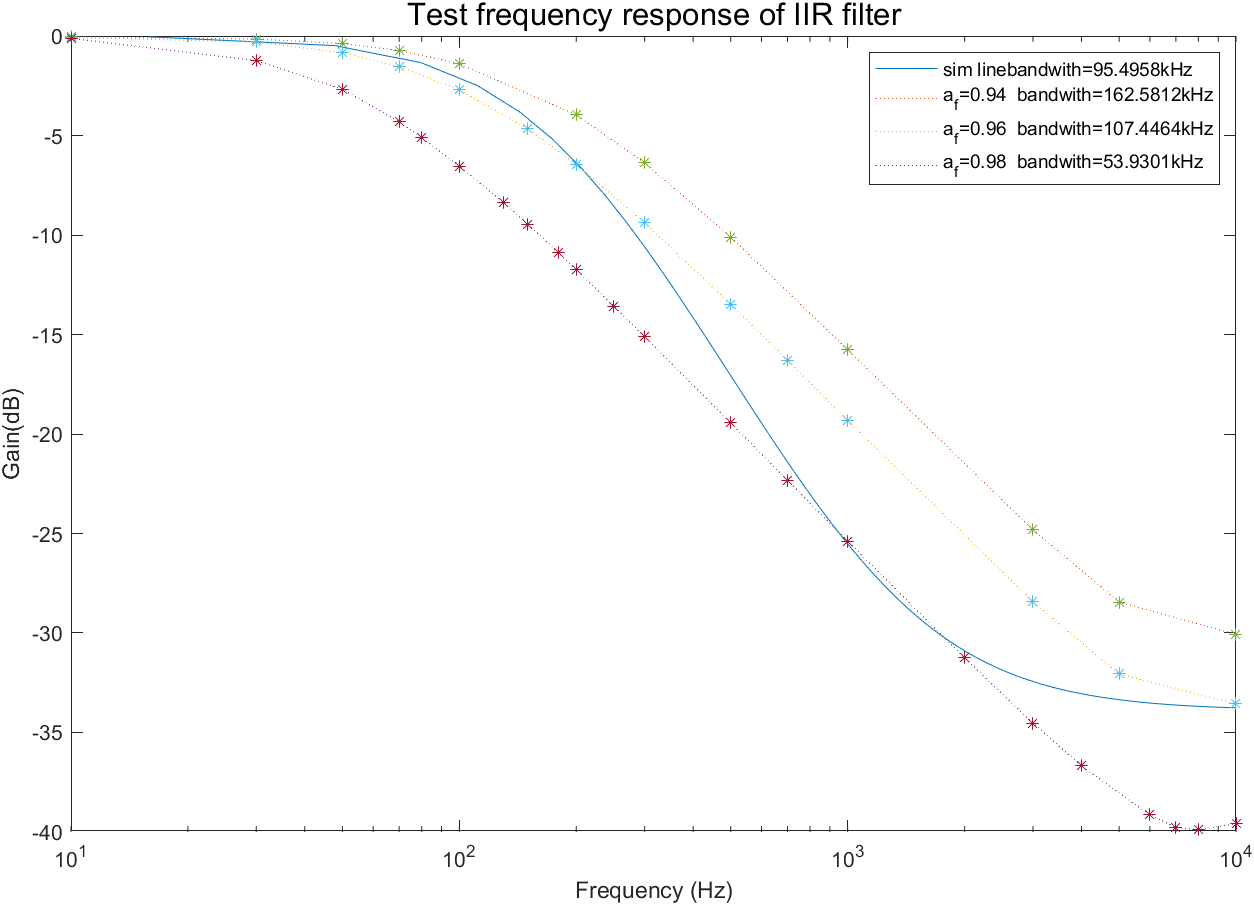
\includegraphics[width=1.0\linewidth]{rtmq/iir_filter_shape}
% \end{figure}
% % !TeX root = ../sustechthesis-example.tex

\chapter[用于离子阱系统的高Q螺线管谐振腔的仿真、优化与建模]{用于离子阱系统的螺线管谐振腔的仿真、优化与建模\label{section:helical}}
% \textcolor{red}{
% 这部分将对之前谐振腔的研究进行整理和总结...
% 除去真空环境相关的部分外,离子阱主要有两核心部分组成:螺线圈谐振腔及刀片阱。
% }
% 如图\ref{fig:quantum_computing_ion_trap_system}显示的,
谐振腔是组成离子阱量子计算系统的重要部分,也是一种十分重要的量子测控器件。在第\ref{section:ion_trap_motion}节中,介绍了离子在离子阱中的囚禁方式和运动,其中囚禁的基础就是生成合适的囚禁势场。在离子阱量子计算实验中通常采用Paul阱来产生这种势场,它也是最具代表性的一类离子阱,利用交替电流(Alternating-Current, AC)电场来动态囚禁带电原子或粒子。上述交流场的频率总是落在射频(RF)范围内,而相应的电压可以达到几百伏。通常,将这种高压射频信号直接应用于Paul阱的电极是具有挑战性的,因为阱本身可以被视为纯电容器件。因此,信号发生器和阱之间的阻抗失配使得功率注入效率低下。

解决上述困难的标准方法是使用螺线管谐振腔来作为信号发生器和离子阱之间的“桥梁”。一个设计合适的螺线管谐振腔既能够实现阻抗匹配的要求也能够放大施加到阱电极上的电场。同时,它还充当带通滤波器来阻断潜在的电子噪声,提高离子量子门的保真度。因此,螺线管谐振腔是离子阱系统中最关键的角色之一,对于特定频率需求范围的谐振腔来说其最关键的参数指标是它的Q值。本章将给出用于离子阱量子计算系统的高Q谐振腔的仿真、设计与优化,以降低噪声提高整个系统的稳定性和离子量子比特操作的保真度\cite[]{van_Dijk_Kawakami_Schouten_Veldhorst_Vandersypen_Babaie_Charbon_Sebastiano_2019},同时也给出一种装配和耦合更方便且更加稳定的模块化谐振腔设计。

% \textcolor{red}{谐振腔与量子门保真度之间的关系说明……}



\section[离子阱系统中的螺线管谐振腔]{离子阱系统中的螺线管谐振腔}

% 如前面在第\ref{section:ion_trap_quantum_computation_system}章中所介绍的,


除去真空环境相关的部分外,离子阱主要有两核心部分组成:螺线圈谐振腔及刀片阱。关于刀片阱的完整设计和制作流程可以参见Myunghun Kim等人\cite[]{Kim_Kim_Hong_Lee_Moon_Lee_Kim_Ha_Sim_Lee_2022}的文章,在此不多赘述。对于螺线管谐振腔,它通常具有两个基本特性,即谐振频率$f_0$和品质因子$Q$。它们的值主要由谐振腔本身的几何设计决定,如图\ref{fig:helical_structure_2d}所示。
对螺线管谐振腔设计的主要目标是找到合适的几何参数,使得谐振频率$f_0$与期望值相匹配,并最大化品质因子$Q$。设计谐振器的一种方法是由其简化的LC电路模型指导,并利用如Macalpine等人\cite[]{Macalpine_Schildknecht_1959}、Deng K.等人\cite[]{Deng_Sun_Yuan_Xu_Zhang_Lu_Luo_2014}给出的经验公式从几何参数估计相应的电容、电感和电阻。
然而,为了使用上述给出的经验公式,某些几何参数之间的比率必须限定于给定的区间,而且估计的$f_0$和$Q$往往与实际值有较大偏差。
近来,一种基于商业软件的有限元(Finite Element, FE)仿真的设计方法开始被广泛使用。Laura Pedrosa-Rodriguez等人\cite[]{Pedrosa_Rodriguez_Outerelo_Gomez_Alcala_de_Vicente_Diaz_Otero_2018}运用解析和数值仿真的方式设计了一种稳定、高电压、高品质因数和低噪声的螺旋管谐振腔,对比结果表明用计算软件对实测样机进行仿真的精度高于解析方程。Joydip Nandi等人\cite[]{Nandi_Sikdar_Reza_Misra_Das_Ray_2020}使用FE的方法设计了一个20MHz的螺旋谐振腔,并通过改变其尺寸和材料对Q值进行了优化。与经验估计方法相比,使用FE方法模拟谐振腔在属性评估方面提供了更高的准确性及灵活性,是一种十分高效且低成本的谐振腔研究设计方法。

\begin{figure}
    \centering
    \caption[谐振腔结构平面示意图]{谐振腔结构平面示意图。$H$:耦合线圈底部到主线圈底部的距离;$B$:屏蔽壳侧壁长度;$D$:屏蔽壳内筒直径;$\tau$:主线圈螺距;$d_0$:主线圈线粗;$d$:主线圈直径;$b$:主线圈总长度;$l_{out}$:输出线长度;$D_1$:输出口内直径。\label{fig:helical_structure_2d}}
    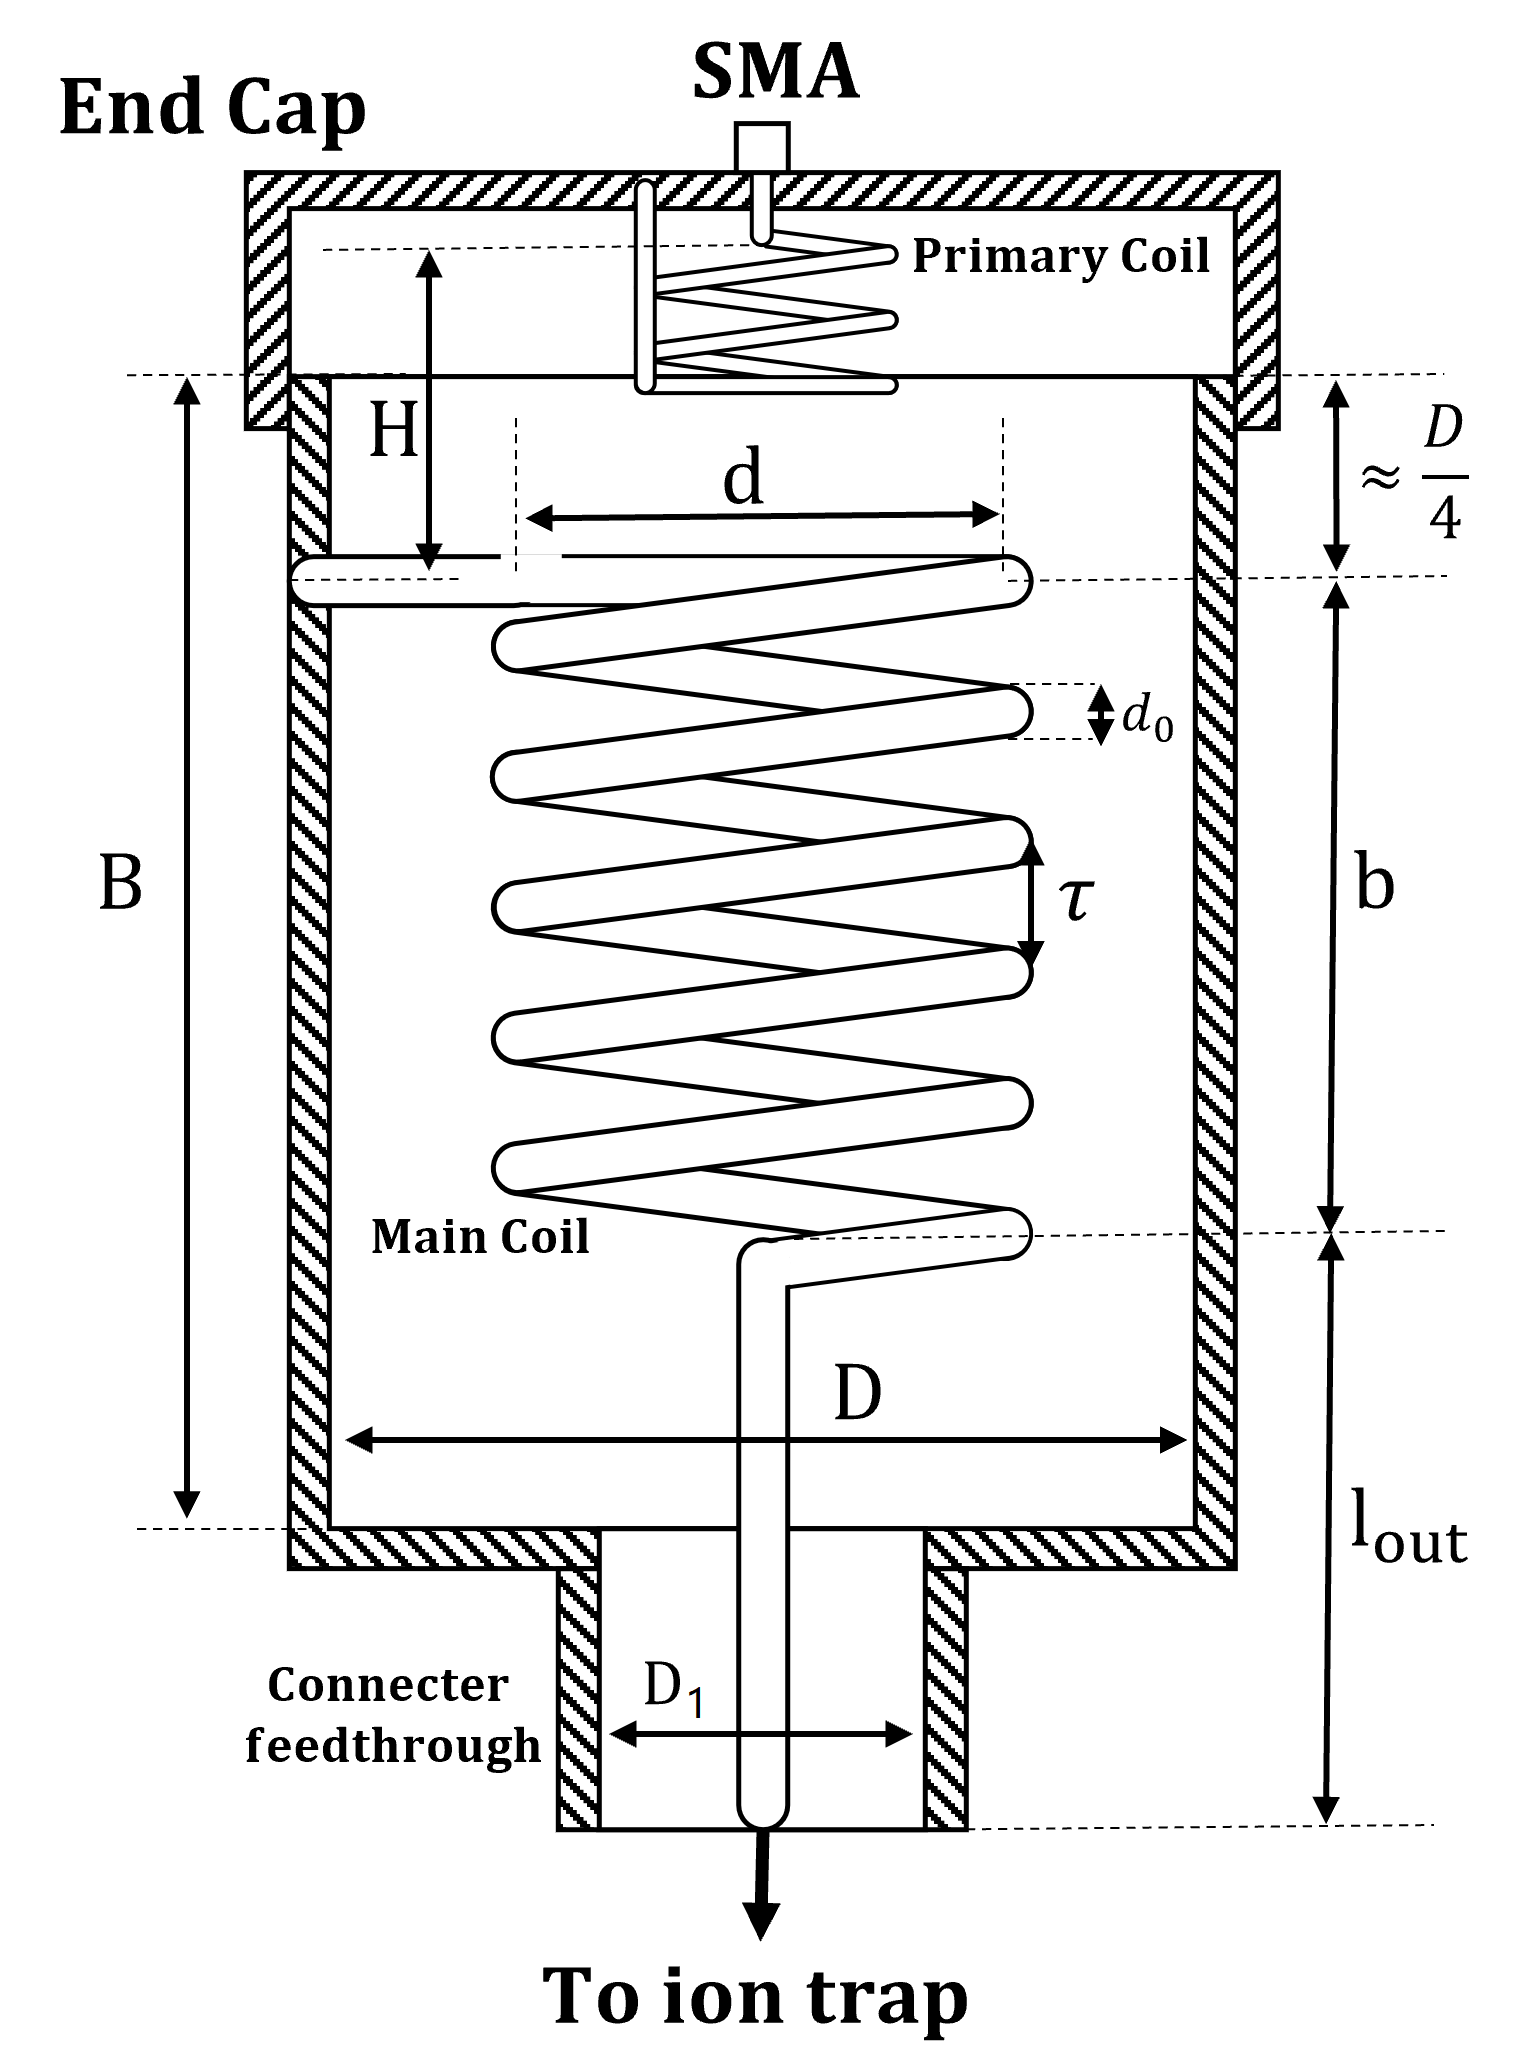
\includegraphics[width=0.5\linewidth]{helical/helical_structure_2d}
\end{figure}

\section[螺线管谐振腔的仿真模型]{螺线管谐振腔的仿真模型}

常用的商业化FE仿真工具有ANSYS HFSS、Comsol等,接下来的仿真中我们采用的ANSYS HFSS来研究影响谐振腔$f_0$和$Q$值的各种因素。在HFSS中,有两种方法可以分析3D结构,本征模模式(Eigen-mode)和驱动模式(Driven-mode)。
本征模模式通过分析计算电磁场模式,直接给出谐振频率$f_0$和品质因子$Q$的结果;而驱动模式是通过设置输入和输出微波端口,分析和计算\emph{散射参数(Scattering Parameter, SP)},与实验更具可比性。
这两种模式都可以用来模拟螺线管谐振腔,但本征模法更常用于谐振器设计,驱动模态在一般仿真中更为频繁。因为驱动模式得到的结果可以直接与实际实验结果做比对,在接下来的仿真研究中我们默认使用这种方法来进行仿真(特别说明的情况除外)。
请注意,由于阻抗匹配网络损耗\cite[]{Gandolfi_Niedermayr_Kumph_Brownnutt_Blatt_2012},驱动模态中品质因子$Q$的结果大约是本征模结果的一半。

我们在仿真软件中构建了与实际谐振器相同的一个3D模型。模型结构示意图如图\ref{fig:helical_structure_2d}所示,HFSS中建立的3D模型视图如图\ref{fig:helical_HFSS_3d}所示。
% ,其表面电流密度矢量分布如图\ref{fig:helical_HFSS_field}所示。
在这个3D模型中,除了主线圈和铜壳结构外,它还包括耦合线圈、输出导线$l_{out}$和连接器馈通结构,3D模型的所有实体结构均为紫铜材料。
主线圈与铜屏蔽壳侧壁接触(gnd);在耦合线圈和主线圈设置两个集总端口,耦合线圈作为输入端口,主线圈作为输出端口,如图\ref{fig:helical_HFSS_3d}中黄色的圆片所示。通过调整耦合线圈到主线圈的距离可以实现阻抗匹配,阻抗匹配的目标是使得S参数反射最小,仿真中采用的标准是$S_{11}<-40$dB。仿真结果的后处理与实际实验完全相同,中心频率$f_0$和$Q$因子可以从$S$参数导出。图\ref{fig:helical_HFSS_field}所展示了谐振腔仿真模型的表面电流密度矢量分布,从图中可以看出表面电流主要分布在主线圈上,谐振腔的损耗主要发生在主线圈上。追求更大的谐振腔Q值本质上就是为了减小谐振腔器件损耗的发生,因此主线圈的材料和结构将是谐振腔研究一个重点的对象。一般来说,制作谐振腔材料的电阻率越小,损耗越小,Q值越大。出于成本和易用性原因,本研究中谐振腔统一采用紫铜材料制作。除此之外,影响谐振腔的Q值的因素主要是其几何结构设计。

\begin{figure}
    \centering
    \caption[HFSS中建立的3D模型图]{HFSS中建立的3D模型图。黄色圆片表示微波输入和输出端口;橙色部分表示耦合线圈和主线圈,一般采用紫铜材质制作;绿色部分是屏蔽外筒,一般采用紫铜或者黄铜制作。\label{fig:helical_HFSS_3d}}
    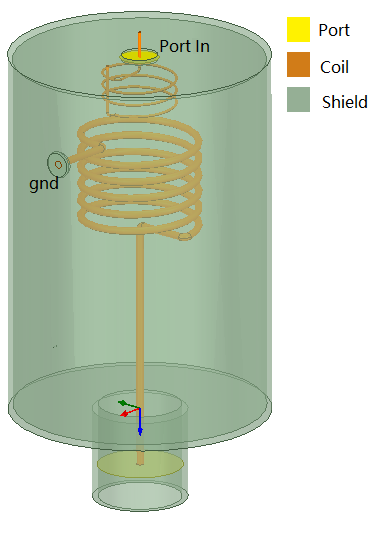
\includegraphics[width=0.4\linewidth]{helical/helical_HFSS_3d}
\end{figure}

\begin{figure}
    \centering
    \caption[HFSS中导出的3D模型表面电流密度矢量图]{HFSS中导出的3D模型表面电流密度矢量图。辅助进行谐振腔的损耗和结构设计分析。从图中可见表面电流主要分布在主线圈上,主线圈的材料和结构是决定谐振腔性能的关键。\label{fig:helical_HFSS_field}}
    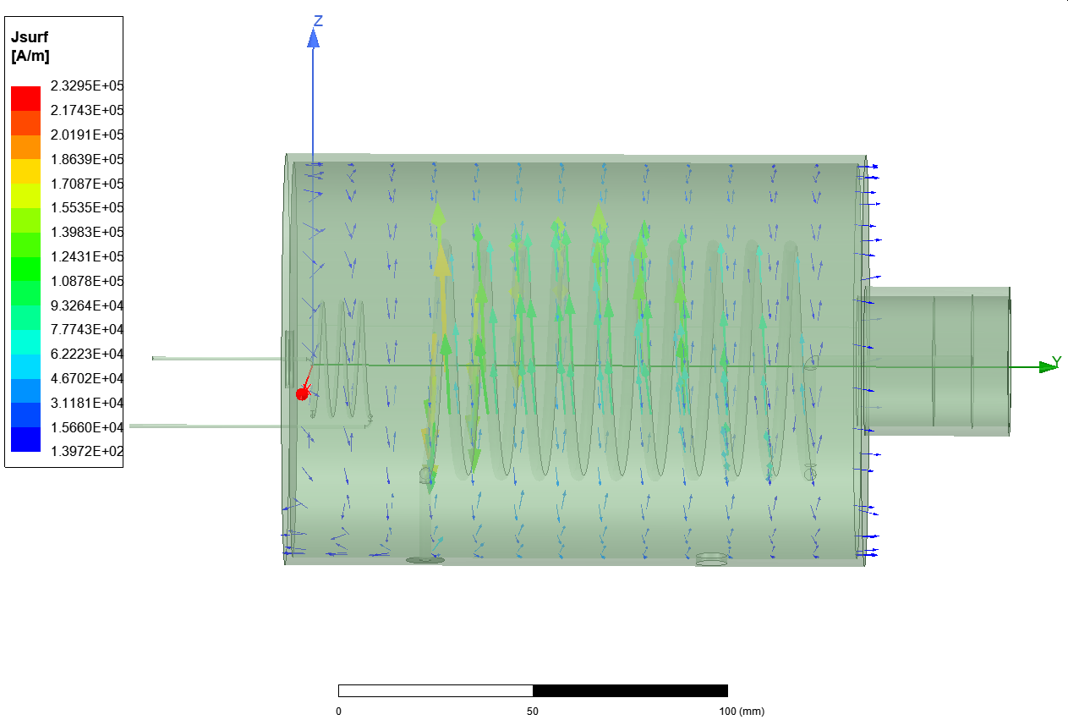
\includegraphics[width=1.0\linewidth]{helical/helical_HFSS_field}
\end{figure}

离子阱实验中的谐振频率通常在$10-100$MHz之间,主线圈的典型直径和螺距间距分别为$50-60 $mm和$5-8$mm。为了测试HFSS模拟和实验之间的一致性,我们选择了三组几何设置,如表\ref{tb:helical_simulation_parameters}所示。
在每个组中,谐振器具有相似的谐振中心频率,但线圈直径和绕组间距不同,即$30$MHz、$50$MHz、$75$MHz组。
除了正常参数外,我们故意选择一个更大的参数范围,接近线圈直径和绕组间距的极限,比如线圈直径在$30-80$mm之间(与屏蔽直径$D=103$mm相比);绕组间距在$4mm$到$ 18$mm之间(与导线直径为$d0 = 3$mm相比)。
关于其它参数,参数$d=48$mm$/\tau = 7$mm的初始轮数$N = 5.734$,屏蔽外壳的高度$ B = 136$mm。螺旋谐振器由网络分析仪Keysight E5063A进行了实验测试。实验测试方案和螺旋谐振器的照片如图\ref{fig:helical_experiment_test}所示。
\begin{table}
    \centering
    \caption[仿真的谐振腔参数设置]{仿真的谐振腔参数设置\label{tb:helical_simulation_parameters}}
    \begin{tabular}{lccccccc}
        %Left\footnote{Note a.}&Centered\footnote{Note b.}&Right\\
        \toprule
        $\#$ & groups & d & $\tau$ & $f_{HFSS}$ & $Q_{HFSS}$ & f$_{exp}$ & $Q_{exp}$ \\
        \midrule

        1 & \multirow{5}{*}{30MHz} 	& 40 & 4  & 32.4062 & 565 & 31.7472 & 513   \\
        2 & 						& 80 & 4  & 25.2663 & 346 & 24.8038 & 207   \\
        3 & 						& 60 & 5  & 28.4732 & 639 & 28.3904 & 587   \\
        4 & 						& 50 & 6  & 30.2228 & 650 & 30.6030 & 599   \\
        5 & 						& 80 & 10 & 27.1943 & 354 & 27.6059 & 317   \\
        \midrule
        6 & 50MHz 					& 48 & 5  & 49.878739 & 708 & 49.2687 & 631   \\
        \midrule
        7 & \multirow{5}{*}{75MHz} 	& 30 & 4  & 76.4602 & 595 & 76.2748 & 542   \\
        8 & 						& 80 & 4  & 61.2866 & 453 & 60.7942 & 389   \\
        9 & 						& 48 & 7  & 74.9382 & 802 & 75.2466 & 708   \\
        10 & 						& 40 & 14 & 88.4308 & 686 & 88.8163 & 571   \\
        11 & 						& 80 & 18 & 77.9517 & 469 & 78.4634 & 377   \\
        \bottomrule
    \end{tabular}
\end{table}


\begin{figure}
    \centering
    \caption[实际实验的测量方式示意图]{实际实验的测量方式示意图。网络分析仪型号为Keysight E5063A。\label{fig:helical_experiment_test}}
    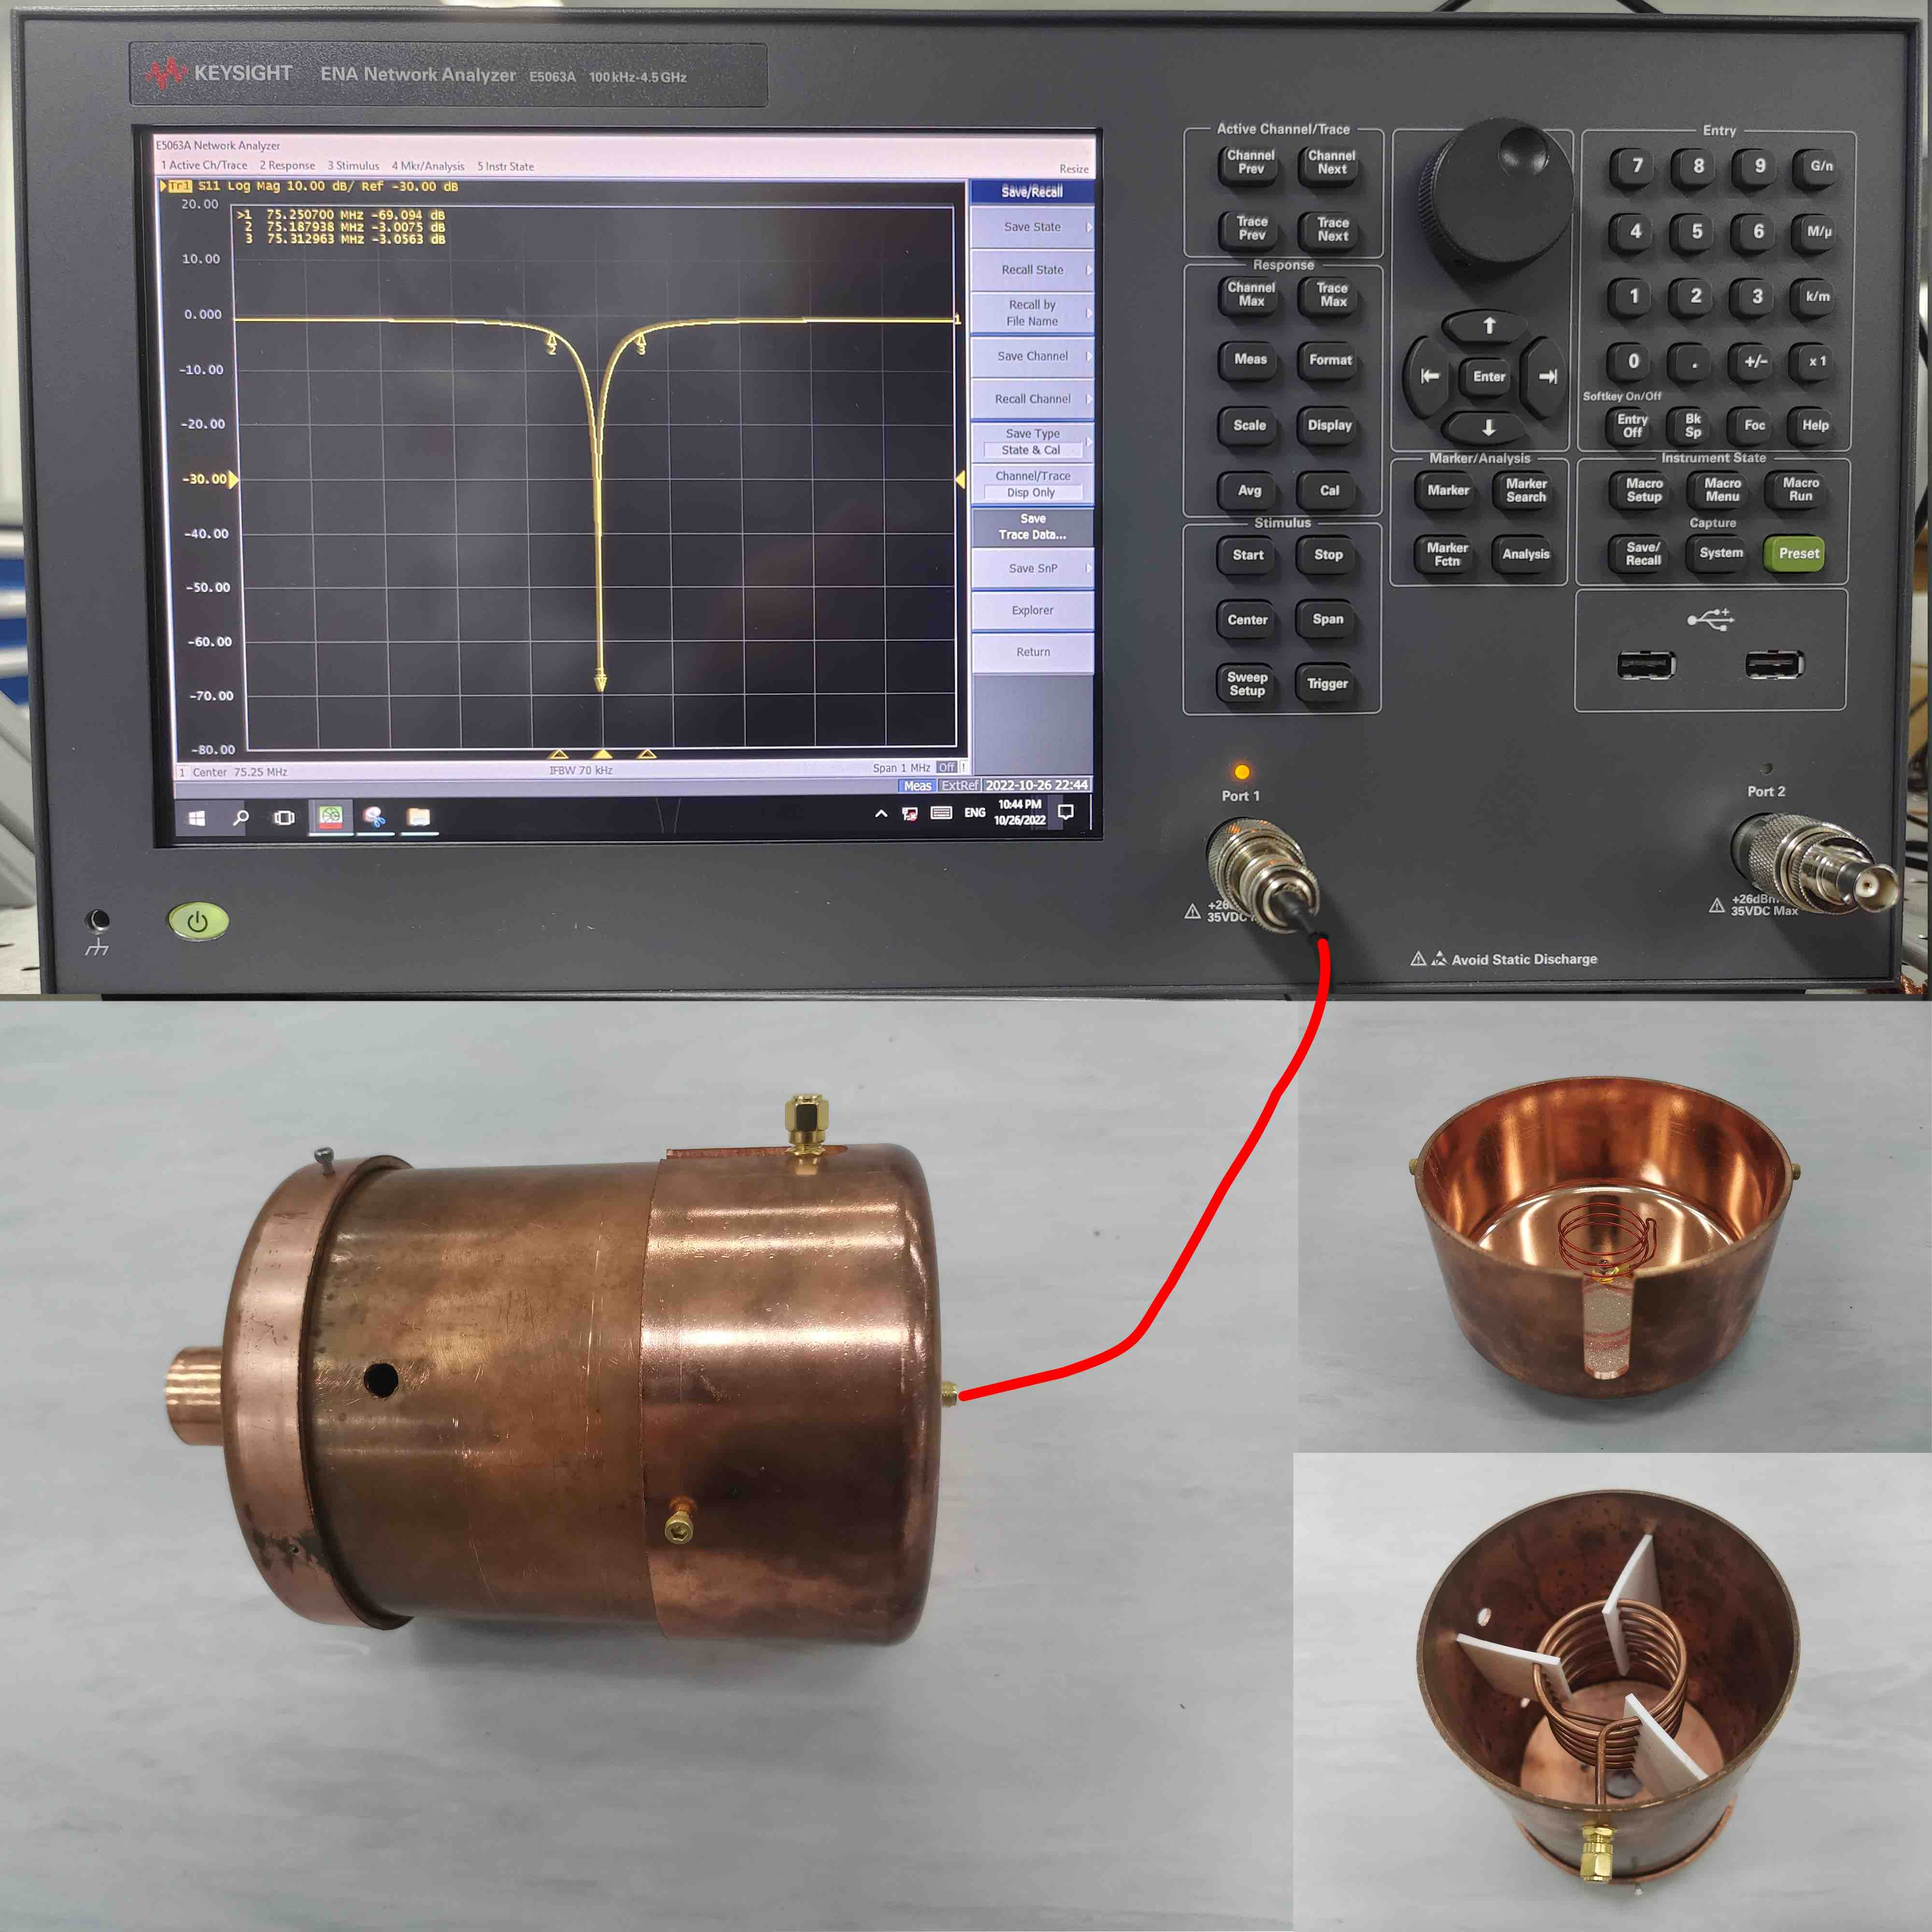
\includegraphics[width=1.0\linewidth]{helical/helical_experiment_test}
\end{figure}

我们选择在表\ref{tb:helical_simulation_parameters}中的2、6、9三行设置作为示例来比较HFSS模拟和实验的结果,散射参数$S_{11}$的对比结果如图\ref{fig:helical_compares}所示(中心频率平移到相互重合,以便清楚地显示$S_{11}$的差异)。结果中的差异$\Delta f(Q)=f(Q)_{exp}-f(Q)_{HFSS}$。实验测试的频率$f_0$和品质因子$Q$结果和误差棒如图\ref{fig:helical_compares_f_q}所示。误差条非常小,几乎不可见。频率的最大差异约为$0.7$MHz。除了一个设置的$Q$因子差为$-122$,其他$Q$因子的差异约为或小于$60$。相对较大的$Q$偏差的原因可能是由于频率和电阻影响。
频率的大小受到电感和电容的影响,电感和电容的具体值由谐振腔的几何结构和材料决定。
电阻受材料和加工过程的影响,例如焊点电阻、金属表面氧化等。此外,我们模拟了我们之前使用的几种螺旋设计,并与实验记录相比,频率差异小于$1$MHz,$Q$差异小于 $50$。

以上结果表明,仿真方法都能较好地预测实验结果。这验证了HFSS商业软件是帮助设计和预测螺旋谐振器行为的绝佳工具,为谐振腔的研究提供了极大的方便。

\begin{figure}
    \centering
    \caption[谐振腔仿真与实验散射参数结果对比]{谐振腔仿真与实验散射参数$S_{11}$结果对比。其中红色实线为HFSS仿真结果,蓝色实线为实验测得的结果。横坐标为频率(单位MHz),纵坐标为幅度(单位dB)。\label{fig:helical_compares}}
    \subcaptionbox[50MHz]{50MHz}{
        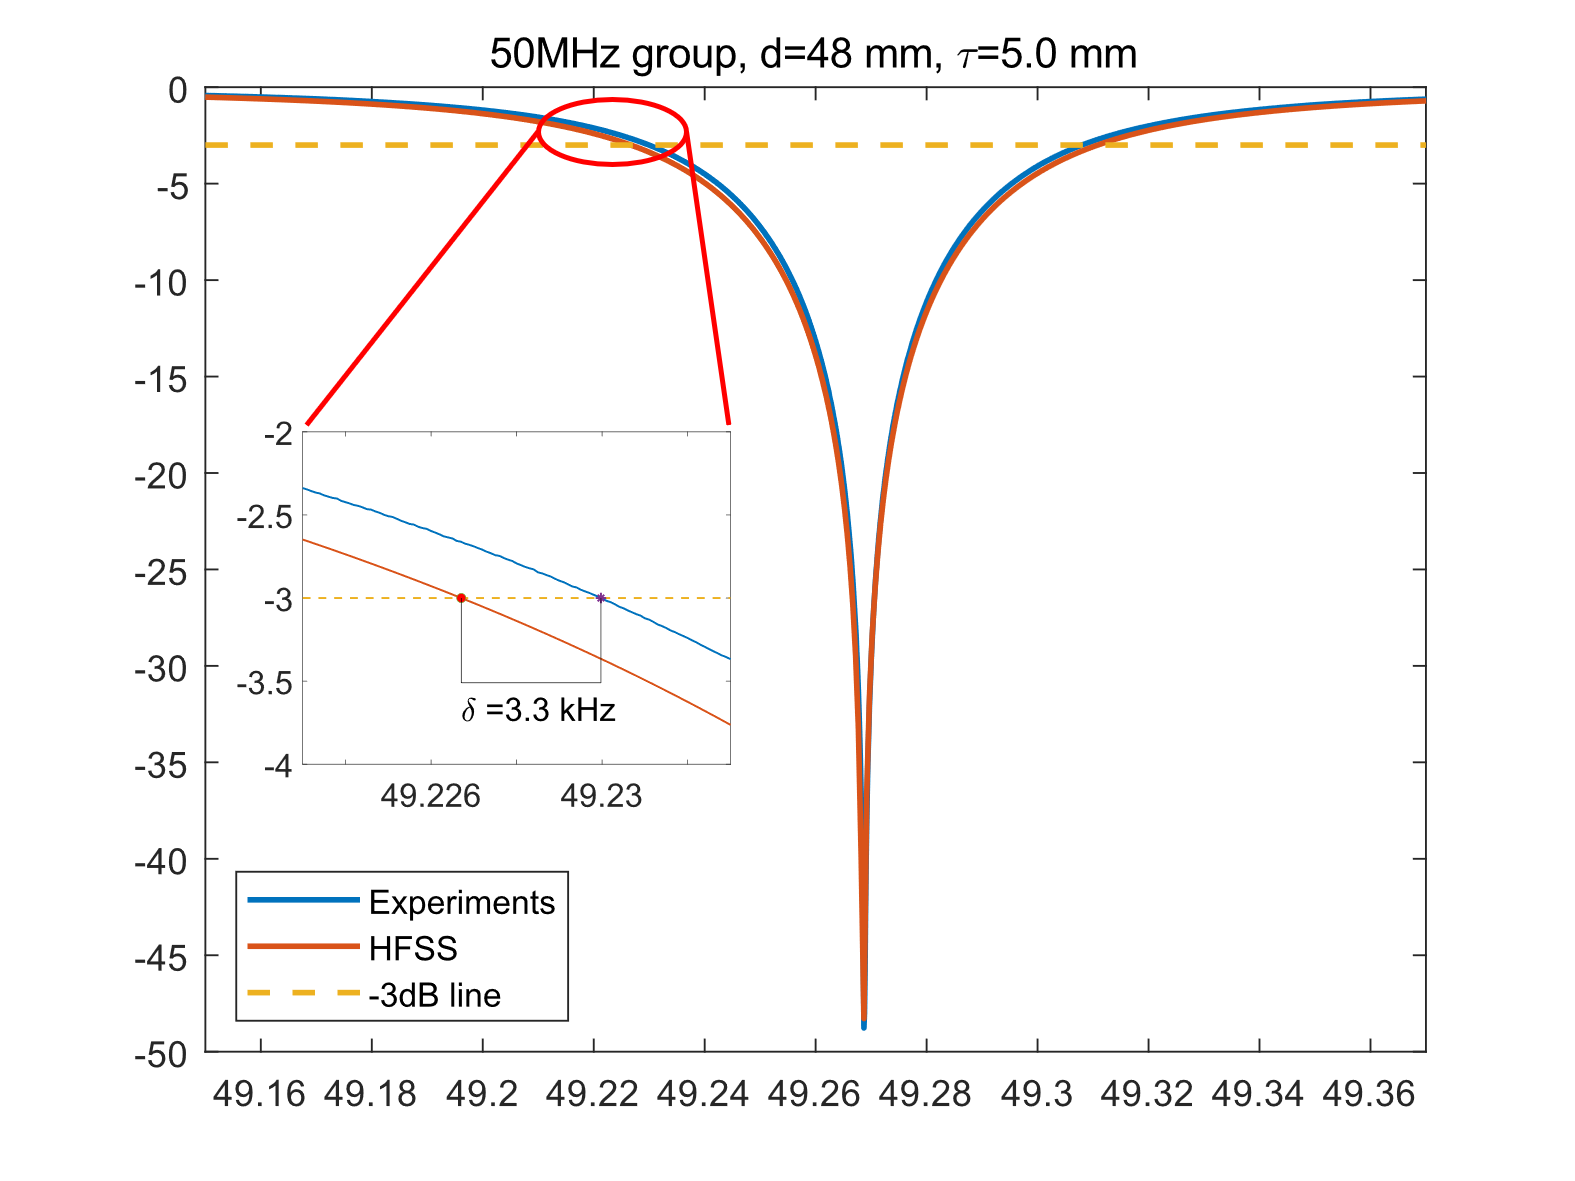
\includegraphics[width=0.8\linewidth]{helical/helical_50MHz_final}
    }
    \subcaptionbox[30MHz]{30MHz}{
        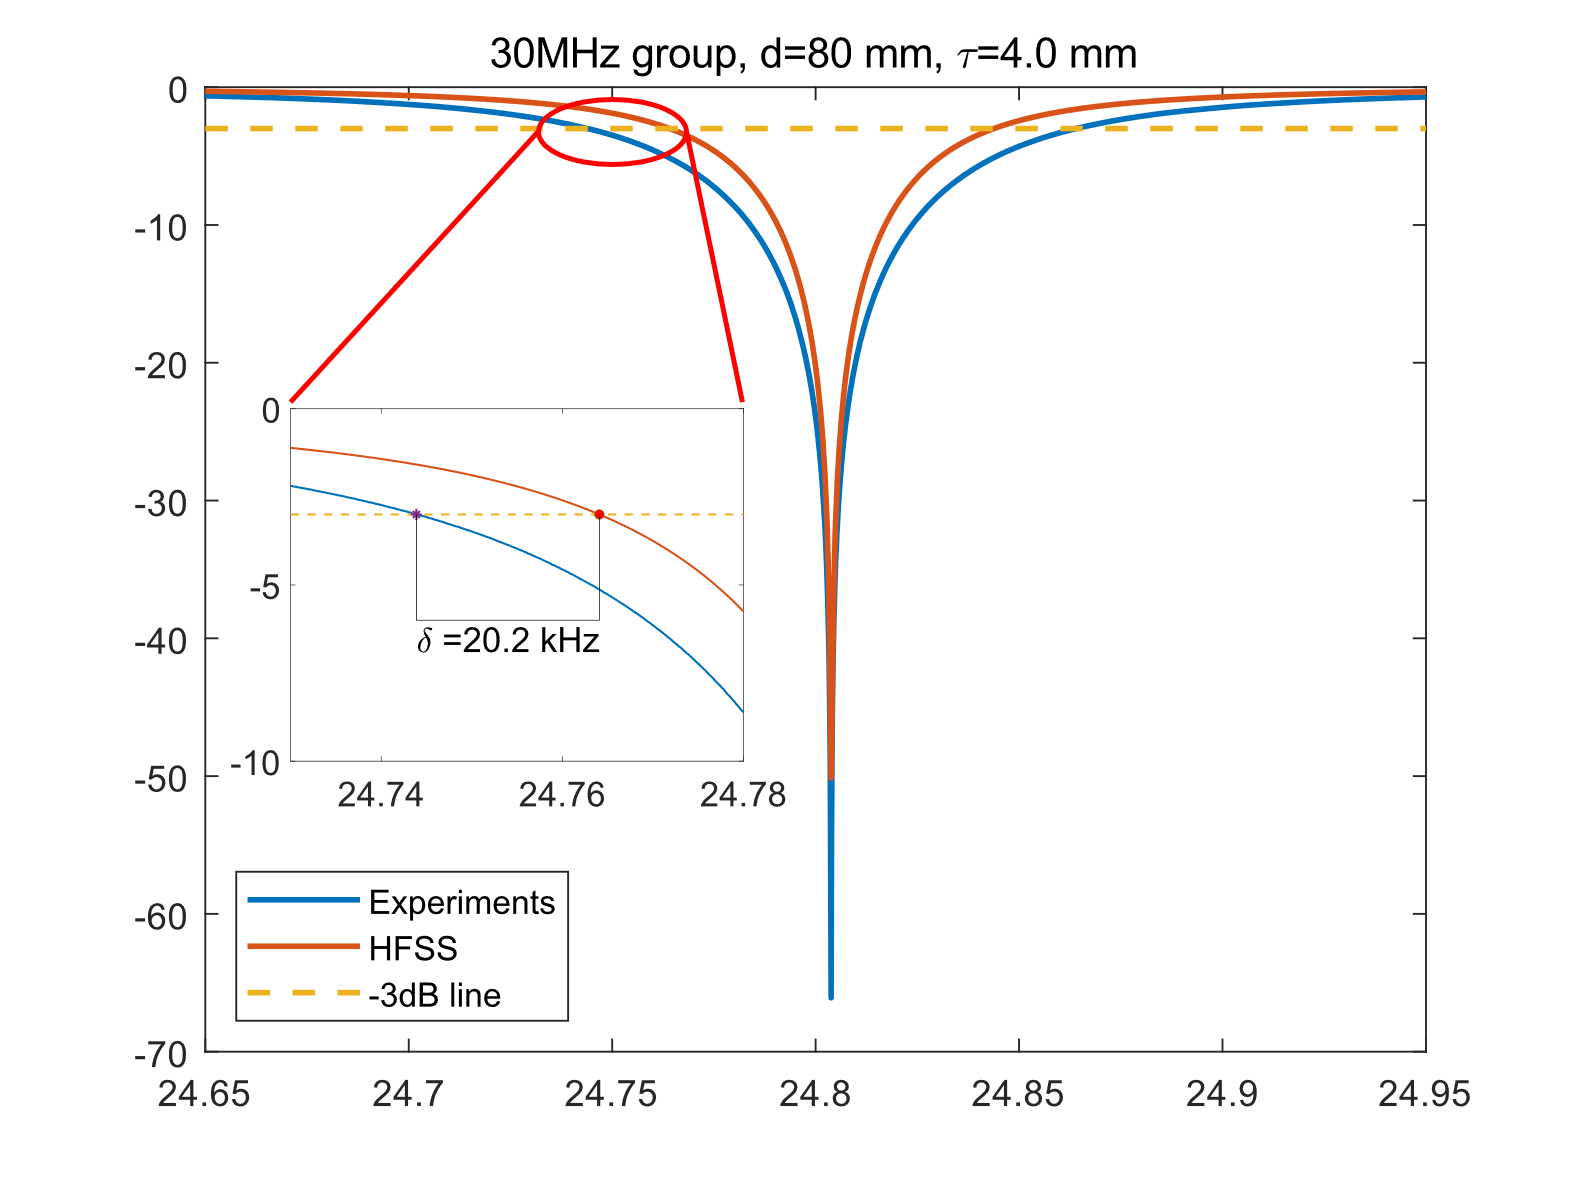
\includegraphics[width=0.46\linewidth]{helical/helical_30MHz_final}
    }
    \subcaptionbox[75MHz]{75MHz}{
        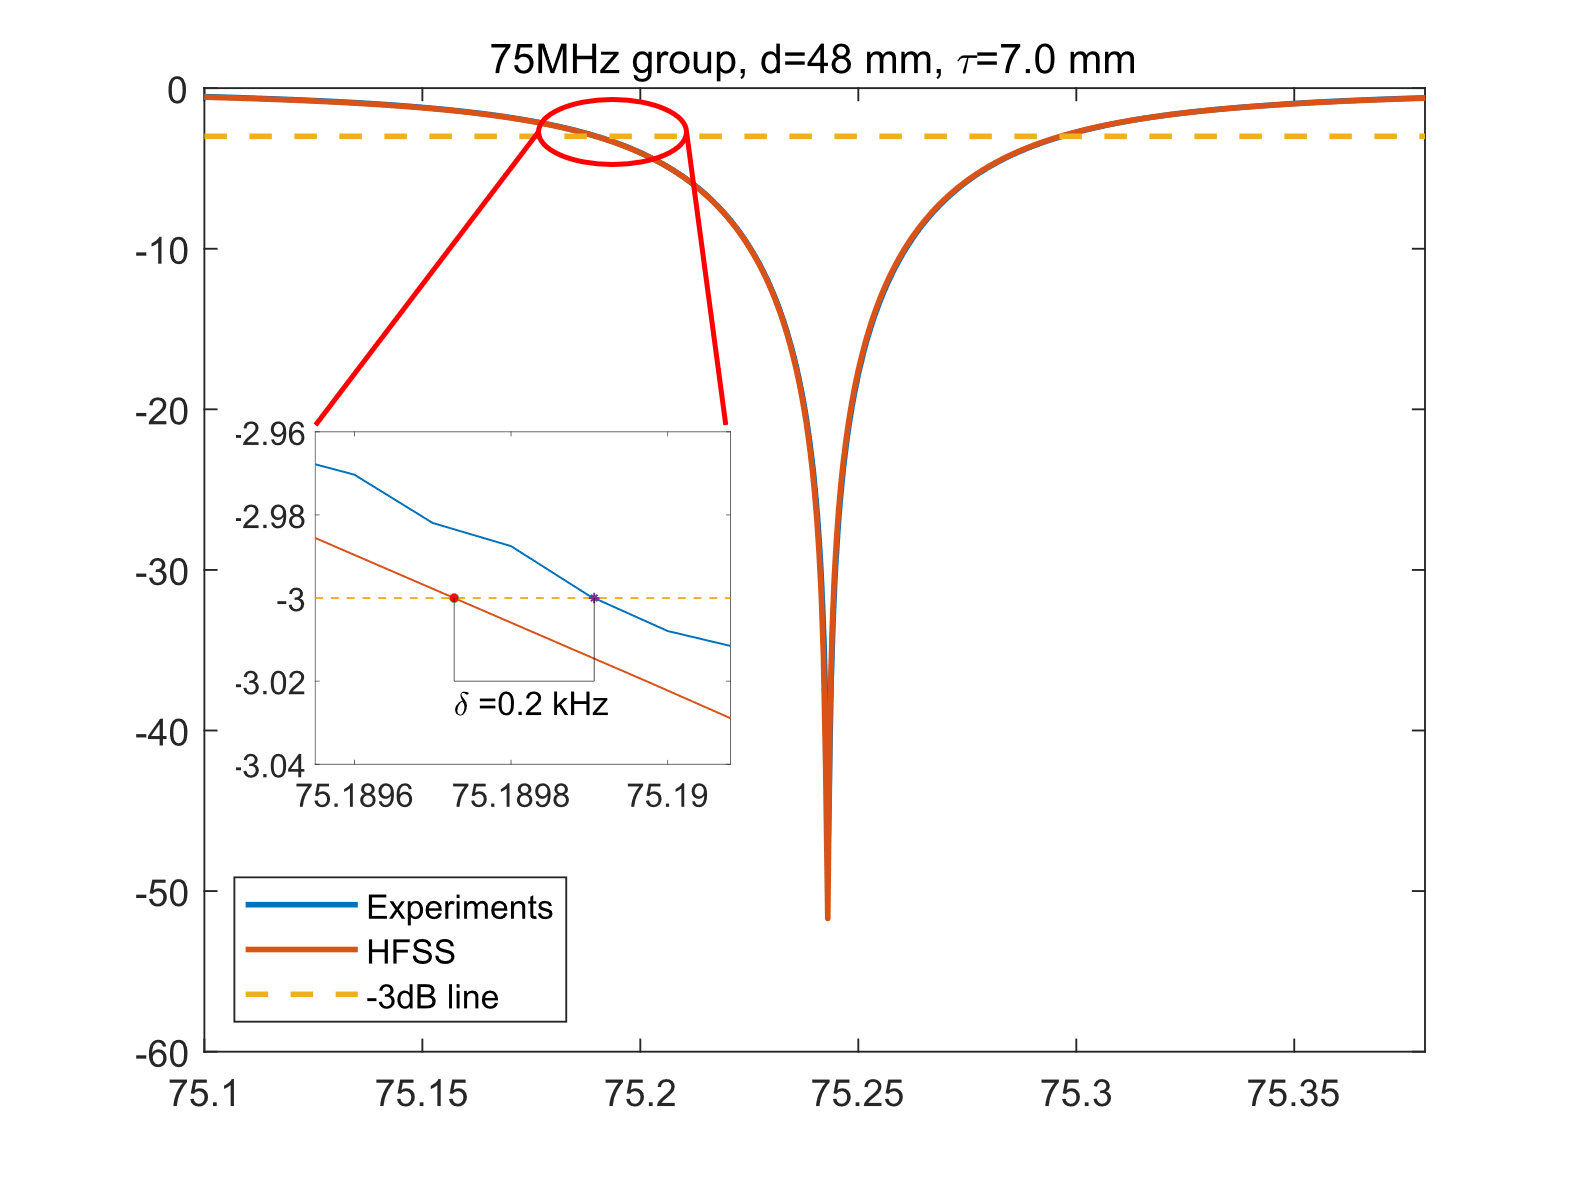
\includegraphics[width=0.46\linewidth]{helical/helical_75MHz_final}
    }
\end{figure}


\begin{figure}
    \centering
    \caption[谐振腔仿真与实验频率和Q结果对比]{谐振腔仿真与实验频率和Q结果对比。横坐标为表中对应的序号数,(a)纵坐标为实验与仿真预测的频率结果偏差$\Delta f$(单位MHz),(b)纵坐标为实验与仿真预测的Q值结果偏差$\Delta Q$(单位1)。\label{fig:helical_compares_f_q}}
    \subcaptionbox[谐振腔仿真与实验频率结果对比]{谐振腔仿真与实验频率结果对比}{
        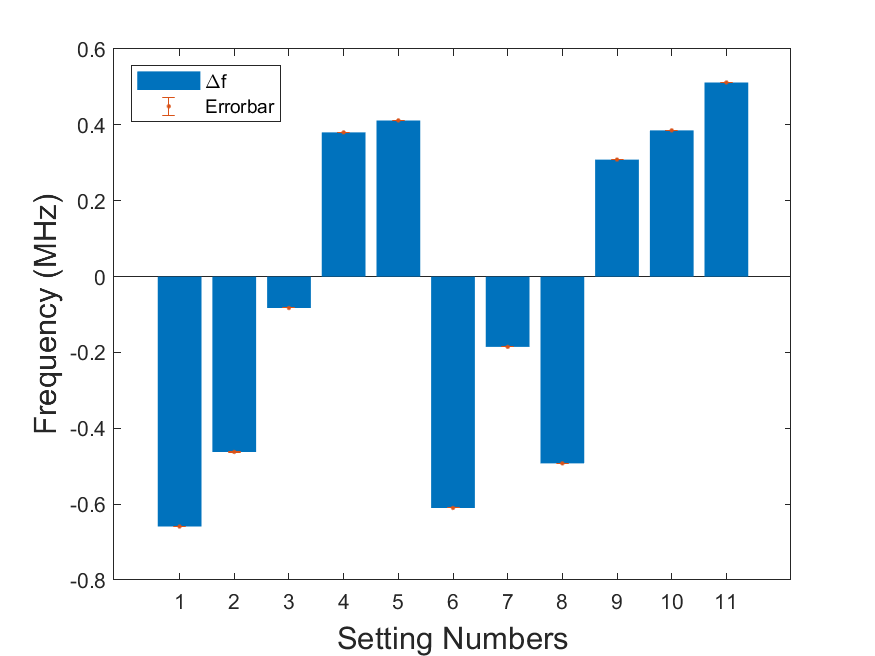
\includegraphics[width=0.48\linewidth]{helical/helical_delta_f}
    }
    \subcaptionbox[谐振腔仿真与实验Q结果对比]{谐振腔仿真与实验Q结果对比}{
        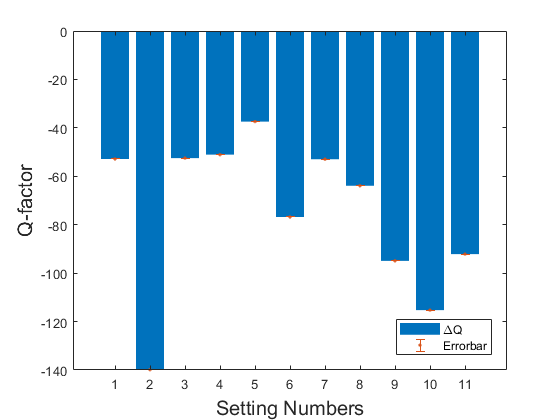
\includegraphics[width=0.48\linewidth]{helical/helical_delta_Q}
    }
\end{figure}

\section[几何参数对频率和Q的影响]{几何维度对频率和Q的影响}

在离子阱的应用中,螺线管谐振腔最重要的性能是谐振频率和Q因子,具有特定谐振频率和最高$Q$因子的谐振腔是最理想的\cite[]{Siverns_Simkins_Weidt_Hensinger_2012}。
谐振频率和Q可以由以下包含集总参数电感$L$、电容$C$和电阻$R$的公式表达:
\begin{align}
    f&=\frac{1}{2\pi\sqrt{LC}} \label{eq:helical_f_equation}\\
	Q&=\frac{\omega L}{R}=\frac{1}{R}\sqrt{\frac{L}{C}} \label{eq:helical_Q_equation}
\end{align}

对于特定的材料,几何物理参数完全决定了设备的所有特性和等效的集总电路参数。进一步地,频率主要取决于电感和电容两者的比值$L/C$,从几何角度看就是取决于谐振腔主线圈的直径、螺距以及总线长等;在此基础上,$Q$除了跟$L/C$有关外,还与电阻有关。
在之前的研究中,大多数研究人员将线圈直径、绕组间距和主线圈数视为非独立参数\cite[]{Siverns_Simkins_Weidt_Hensinger_2012,Macalpine_Schildknecht_1959}。
然而,在我们的模拟中,我们发现如果主线圈的总长度是固定的,谐振频率将比总导线长度变化小得多,结果如图\ref{fig:helical_fixedwirelength}所示。
这使得谐振频率的控制更容易。一项研究\cite[]{Nandi_Sikdar_Das_Ray_2022}也指出了这种类似的现象,它给出了谐振频率与主线圈长度之间的关系。螺线管谐振腔基本上与四分之一波长谐振器相同。
\begin{figure}
    \centering
    \caption[固定线长下改变主线圈参数的频率$f_0$变化]{固定线长下改变主线圈参数的频率$f_0$变化。(a)横坐标为主线圈直径$d$(单位mm),(b)主线圈螺距$\tau$(单位mm);纵坐标为频率$F$(单位MHz)。\label{fig:helical_fixedwirelength}}
    \subcaptionbox[改变主线圈直径参数]{改变主线圈直径参数}{
        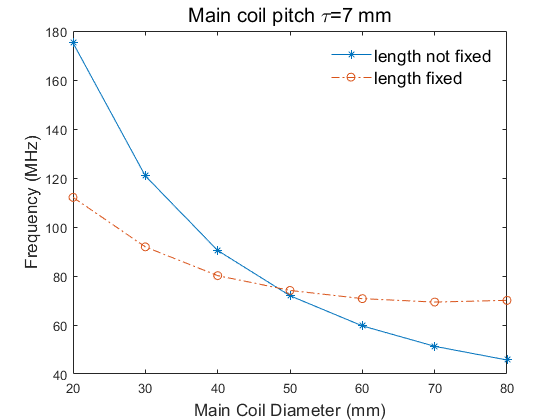
\includegraphics[width=0.48\linewidth]{helical/helical_fixedwirelength_1}
    }
    \subcaptionbox[改变主线圈螺距参数]{改变主线圈螺距参数}{
        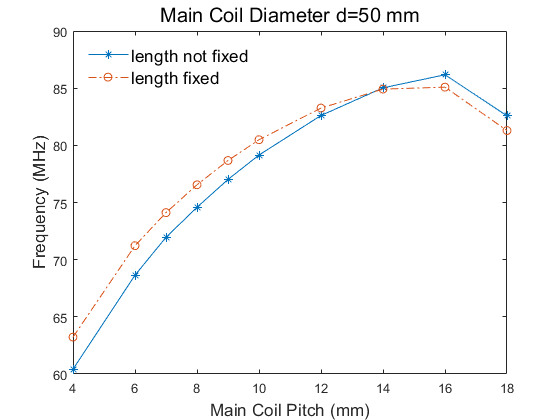
\includegraphics[width=0.48\linewidth]{helical/helical_fixedwirelength_2}
    }
\end{figure}

在我们的模拟中,主要线圈几何形状设置了两个限制,即固定的总导线长度$l_{total}$和固定的总导线高度$h$:
\begin{align}
    l_{total}&=N\sqrt{(\pi d)^2+\tau^2}+l_{out} \label{eq:helical_fixed_constraints_1}\\
	h&=N\tau+l_{out} \label{eq:helical_fixed_constraints_2}
\end{align}

因此,频率在$d=20 $mm到$d=80 $mm时平均变化约为$0.701$MHz/mm;虽然绕组间距效应不那么明显,但频率在$\tau=4 $mm到$\tau=118 $mm时平均变化约为$1.29$MHz/mm。这种现象有助于分离几何效应和频率变化之间$ Q $因子改进的原因。接下来的几节将在这些预设下,研究几个几何参数的效应来设计所需的频率$f_0$和$Q$因子。
\subsection[主线圈几何参数的影响]{主线圈几何参数的影响}

为了研究对谐振频率$f_0$和$Q$因子的几何效应,基于表\ref{tb:helical_simulation_parameters}中第9行的参数,对几组主线圈参数进行设置和模拟。
主线圈的直径和间距设置为双参数扫描;直径从$30-80$mm,步长为$10$mm;螺距设置为$4-18$mm,步长为$2$mm。
这些模拟的结果给出了一个谐振频率$f_0$和$Q$因子的几何效应图,将其绘制为等高线图,如图\ref{fig:helical_contour}所示。左上角的白色三角形是参数禁止区,因为主线圈参数不满足约束公式\eqref{eq:helical_fixed_constraints_1}和\eqref{eq:helical_fixed_constraints_2}。
使用一组确定的参数($d$和$\tau$),可以近似在这个等高线图上立即读出谐振频率$f_0$和$Q$因子,如图中红点代表表\ref{tb:helical_simulation_parameters}中第9行的参数设置。

\begin{figure}
    \centering
    \caption[螺线管谐振腔$f_0$、$Q$值等高图]{螺线管谐振腔$f_0$、$Q$值等高图。横坐标为主线圈直径$d$(单位mm),纵坐标为主线圈螺距$\tau$(单位mm)\label{fig:helical_contour}}
    \subcaptionbox[螺线管谐振腔$f_0$值等高图]{螺线管谐振腔$f_0$值等高图\label{fig:helical_contour_f}}{
        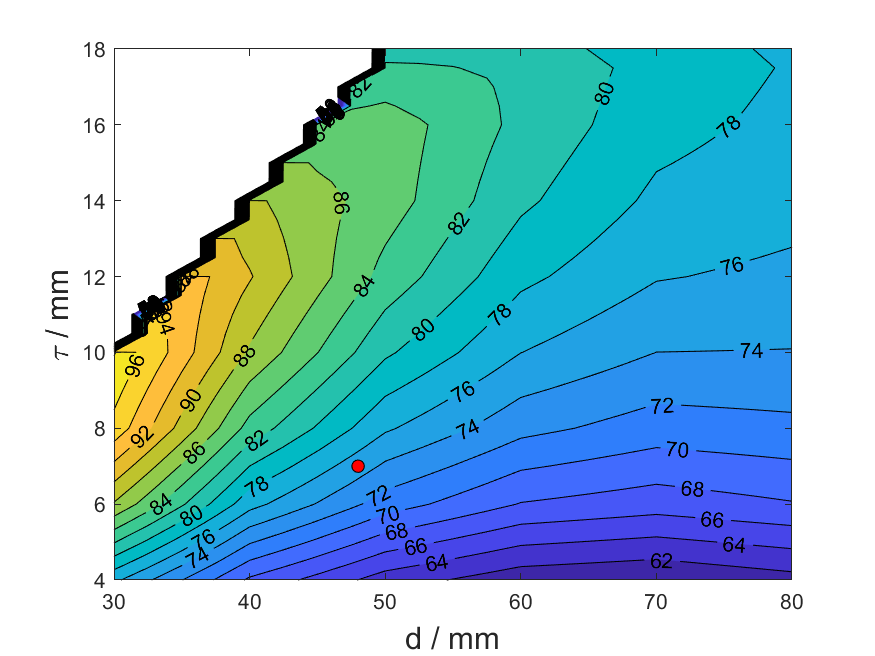
\includegraphics[width=0.48\linewidth]{helical/helical_contour_f}
    }
    \subcaptionbox[螺线管谐振腔$Q$值等高图]{螺线管谐振腔$Q$值等高图\label{fig:helical_contour_Q}}{
        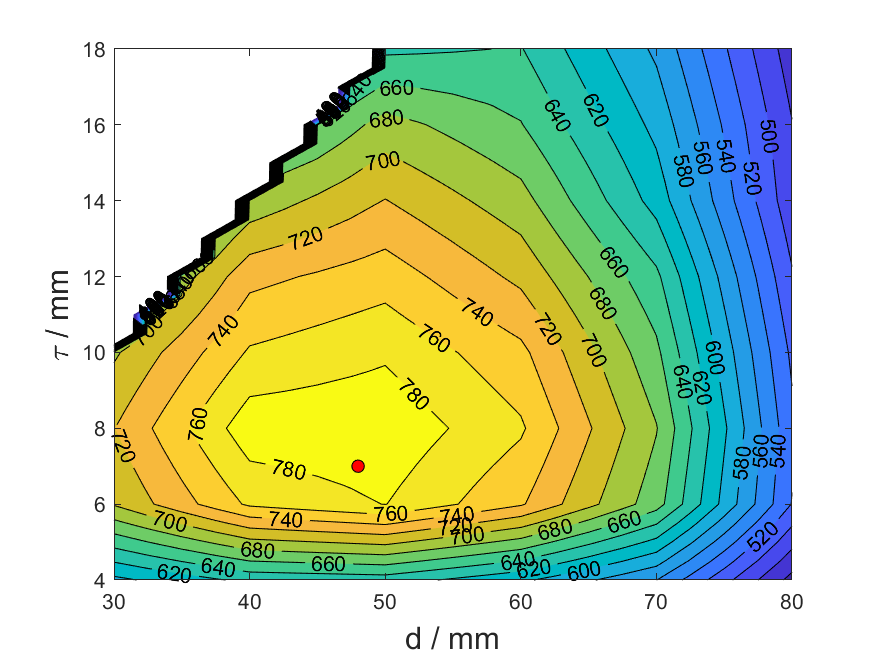
\includegraphics[width=0.48\linewidth]{helical/helical_contour_Q}
    }
\end{figure}

在图\ref{fig:helical_contour_f}中,频率$f_0$在绝大部分地方随着$\tau$的减小而减小。随着主线圈直径$d$的增加,电感$L$会先慢慢增加(当$d$较小时)然后减小(当$d$较大时)。同时,$C_c$和$C_s$单调地增加。因此在这个过程中频率会先急剧下降然后慢慢下降。参考频率计算公式\eqref{eq:helical_f_equation}和文献\cite[]{Siverns_Simkins_Weidt_Hensinger_2012,Macalpine_Schildknecht_1959}中的电感$L$和电容$C = C_c +C_s$计算公式:
\begin{align}
    L&=39.37b\frac{0.025d^2(1-(\frac{d}{D})^2)}{\tau^2} &\mu \textnormal{H/m} \label{eq:helical_L} \\
	C_c&=d(11.26\frac{b}{d}+8+\frac{27}{\sqrt{b/d}})  &\textnormal{pF/m} \label{eq:helical_C_c}\\
	C_s&=39.37b\frac{0.75}{lg(D/d)} &\textnormal{pF/m} \label{eq:helical_C_s}
\end{align}

然而,在左上和右下角,有两个非单调异常区域。一种是在大$d$和小$\tau$参数区(右下区域)。
频率等高线不是单调的,随着$d$的增大等高线向下弯曲。
这是因为当单独改变$d$时$L$有一个最大值,并且由$\tau$导致的$L$变化不足以逆转这个最大值附近的影响。另一处是在小$d$和大$\tau$参数区(左上区域)。在这里频率等高线也不是单调的,随着$\tau$的增大等高线向左弯曲(如果是将$\tau$作为横轴则是向下弯曲)。这是因为当$\tau$过大时会螺线圈会更加接近输出端会更加接近屏蔽壳引入较大的侧壁电容$C_s$而增大$\tau$带来的电感减少效应不足以抵消,从而导致频率未能随$\tau$单调增加。

对于$Q$的变化,如图\ref{fig:helical_contour_Q}所示,它具有一个明显的最大值。可见选择合适的$d$和$\tau$是十分重要的。图中$Q$的最大值位置约在$d=48$mm,$\tau=7.3$mm处,最大值$Q$约为$810$。图中红点表示了表\ref{tb:helical_simulation_parameters}中第9行的参数的$Q$值结果。

在图\ref{fig:helical_contour}的$ f_0,\ Q $结果图的帮助下,可以直接读出具有特定几何参数设置的任何$f_0$和$Q$结果。该图还可以帮助谐振腔设计和确定的$f_0$和$Q$。
此外,沿$d$或$\tau$方向任意点的偏导数将给出线圈参数对频率和$Q$的敏感性。几何参数对$f,\ Q$的敏感性决定了线圈的加工精度,以及实验误差范围。
以图\ref{fig:helical_contour}中的红点参数为例,计算线圈$d$和$\tau$灵敏度,结果如表\ref{tb:helical_d_tau_sensitivity}所示。
从结果中可以看出,灵敏度$d$的结果值小于$\tau$的结果值。因此,在加工过程中,$\tau$大小的偏差更有可能对 $f,\ Q$产生影响,值得更多地关注。

\begin{table}
    \centering
    \caption[谐振腔对主线圈直径和螺距参数的敏感性]{谐振腔对主线圈直径和螺距参数的敏感性\label{tb:helical_d_tau_sensitivity}}
    \begin{tabular}{ccccc}
        \toprule
        Operation & range (mm) & F sensitivity(MHz/mm) & Q sensitivity (/mm) \\
        \midrule
        $d$ Stretch & [-1,1] & $\approx$-0.606 & $\approx$ 0.4\\
        $\tau$ Stretch & [0, 0.5] & $\approx$ 2.988 & $\approx$ 23.491 \\
        Axial Shift & [-2, 2] & $\approx$ -0.049 & $\approx$ 0.185\\
        Radial Shift & [-2, 2] & $\approx$ 0.034 & $\approx$ -0.4904\\
        \bottomrule
    \end{tabular}
\end{table}

除了研究$f,\ Q$的独立参数变化效应外,我们还研究了主线圈平移对$f,\ Q$的影响,即沿径向或轴向。结果如图\ref{fig:helical_bias_axial}、图\ref{fig:helical_bias_radial_gndalong}、图\ref{fig:helical_bias_radial_gndperpendicular}和表\ref{tb:helical_d_tau_sensitivity}所示。
从结果可以看出,主线圈的轴向平移和径向平移对$f,\ Q$影响不大。平移对$f,\ Q$的影响远小于几何参数 ($d,\ \tau$) 变化效应。因此,我们需要更多地关注加工过程中主线圈的俯仰精度,以获得更一致的实验结果。

\begin{figure}
    \centering
    \caption[谐振腔仿真与实验结果对比——主线圈轴向偏移]{谐振腔仿真与实验结果对比——主线圈轴向偏移。\label{fig:helical_bias_axial}}
    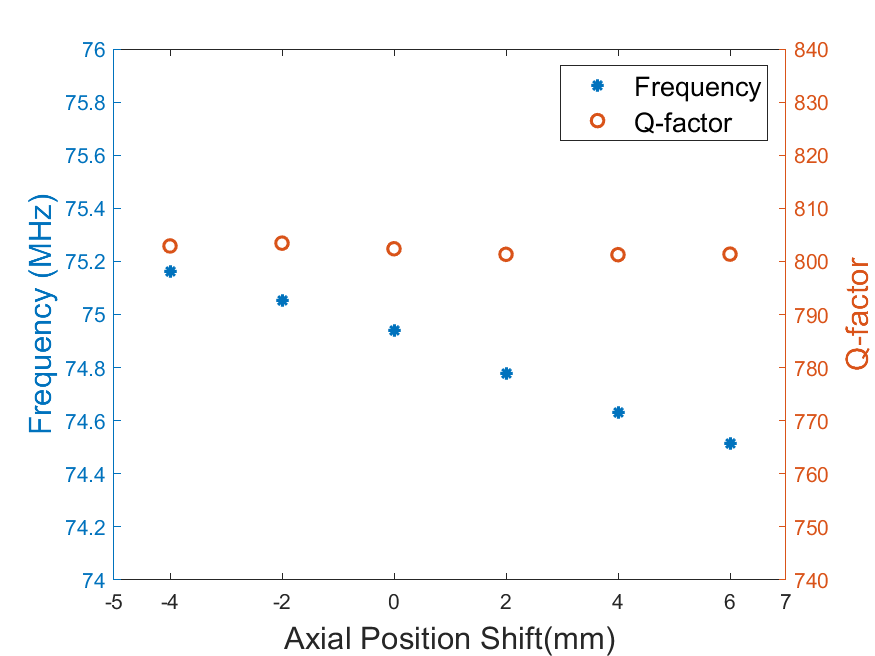
\includegraphics[width=0.8\linewidth]{helical/helical_bias_axial}
\end{figure}

\begin{figure}
    \centering
    \caption[谐振腔仿真与实验结果对比——主线圈径向偏移(垂直于接地端)]{谐振腔仿真与实验结果对比——主线圈径向偏移(垂直于接地端)。\label{fig:helical_bias_radial_gndalong}}
    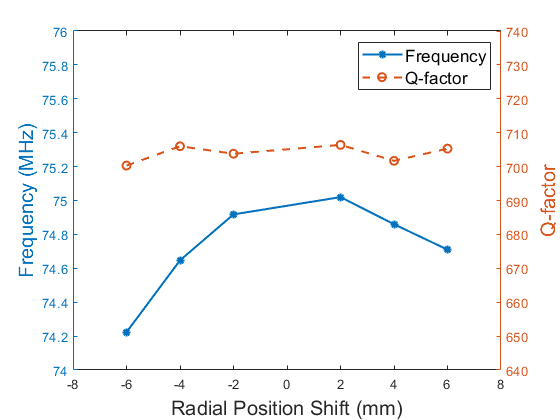
\includegraphics[width=0.8\linewidth]{helical/helical_bias_radial_gndalong}
\end{figure}

\begin{figure}
    \centering
    \caption[谐振腔仿真与实验结果对比——主线圈径向偏移(垂直于接地端)]{谐振腔仿真与实验结果对比——主线圈径向偏移(垂直于接地端)。\label{fig:helical_bias_radial_gndperpendicular}}
    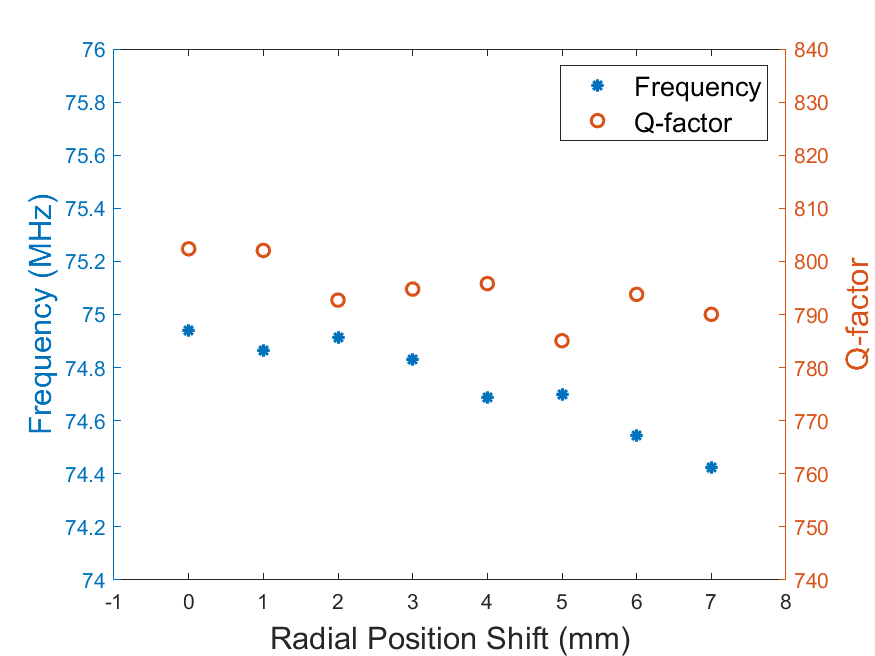
\includegraphics[width=0.8\linewidth]{helical/helical_bias_radial_gndperpendicular}
\end{figure}


% \begin{figure}
%     \centering
%     \caption[谐振腔仿真与实验散射参数结果对比]{谐振腔仿真与实验结果对比。(a)横坐标为主线圈轴向偏移距离(单位mm),(b)主线圈平行于接地端径向偏移(单位mm),(c)主线圈垂直于接地端径向偏移(单位mm)。\label{fig:helical_main_coil_compares}}
%     \subcaptionbox[主线圈轴向偏移]{主线圈轴向偏移\label{fig:helical_bias_axial}}{
%         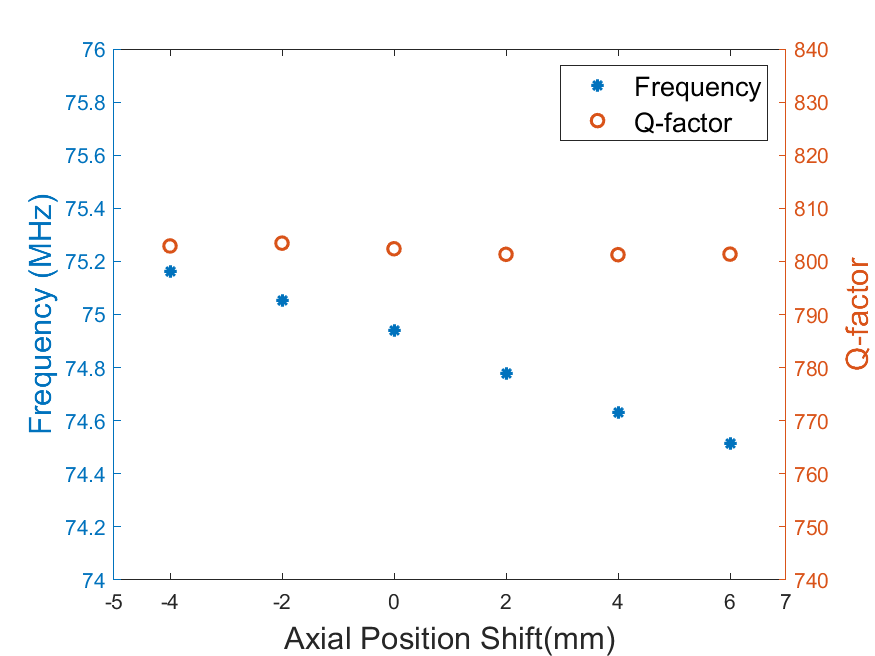
\includegraphics[width=0.8\linewidth]{helical/helical_bias_axial}
%     }
%     \subcaptionbox[主线圈径向偏移(平行于接地端)]{主线圈径向偏移(平行于接地端)}{
%         %0.46 for two
%         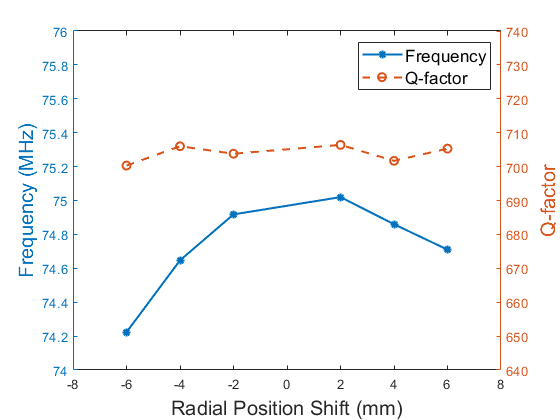
\includegraphics[width=0.8\linewidth]{helical/helical_bias_radial_gndalong}
%     }
%     \subcaptionbox[主线圈径向偏移(垂直于接地端)]{主线圈径向偏移(垂直于接地端)}{
%         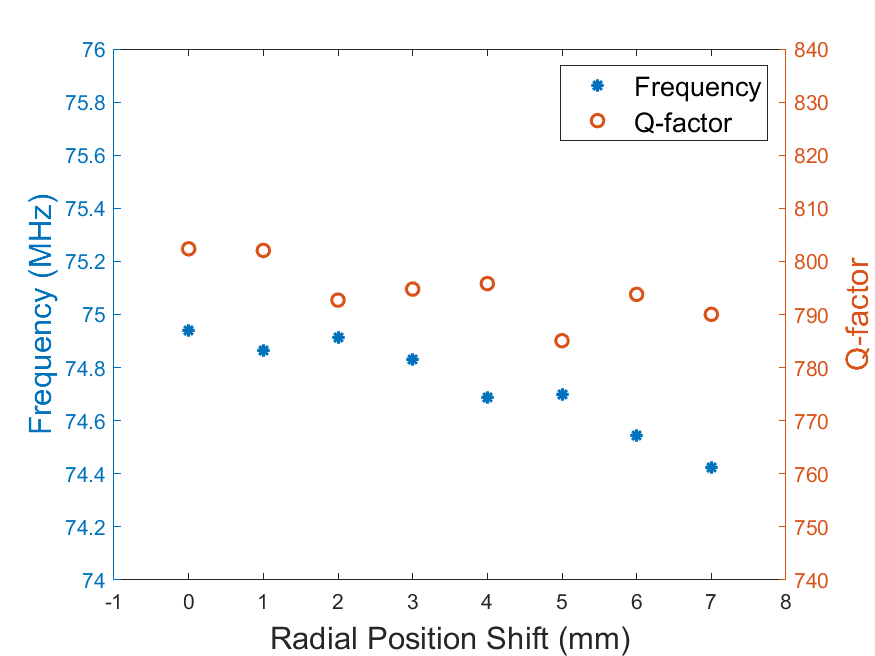
\includegraphics[width=0.8\linewidth]{helical/helical_bias_radial_gndperpendicular}
%     }
% \end{figure}


\subsection[输出线参数的影响]{输出线参数的影响\label{section:helical_output_wire}}
在我们的模拟中,我们发现输出导线长度对谐振$f,\ Q$有很大的影响。与之前的固定线长情况不同,这里我们不再做公式\eqref{eq:helical_fixed_constraints_1}和公式\eqref{eq:helical_fixed_constraints_2}的约束。
主线圈直径及其螺距保持在相同的长度,独立改变输出导线$l_{out}$的总长度,其中$l_{out} = l_{lout1} + l_{lout2}$。
$l_{out1}$和$l_{out2}$分别是屏蔽外壳中的输出线和连接器馈通部分的输出线,如图\ref{fig:helical_lout_2}所示。


\begin{figure}
    \centering
    \caption[输出线部分示意图]{输出线部分示意图。$l_{out1}$:输出线在屏蔽壳内部分的长度;$C_{lout1}$:输出线在屏蔽壳内部分的电容;$l_{out2}$:输出线在输出端口内部分的长度;$C_{lout2}$:输出线在输出端口内部分的电容;$D$:屏蔽壳内直径;$D_1$:输出端内直径。\label{fig:helical_lout_2}}
    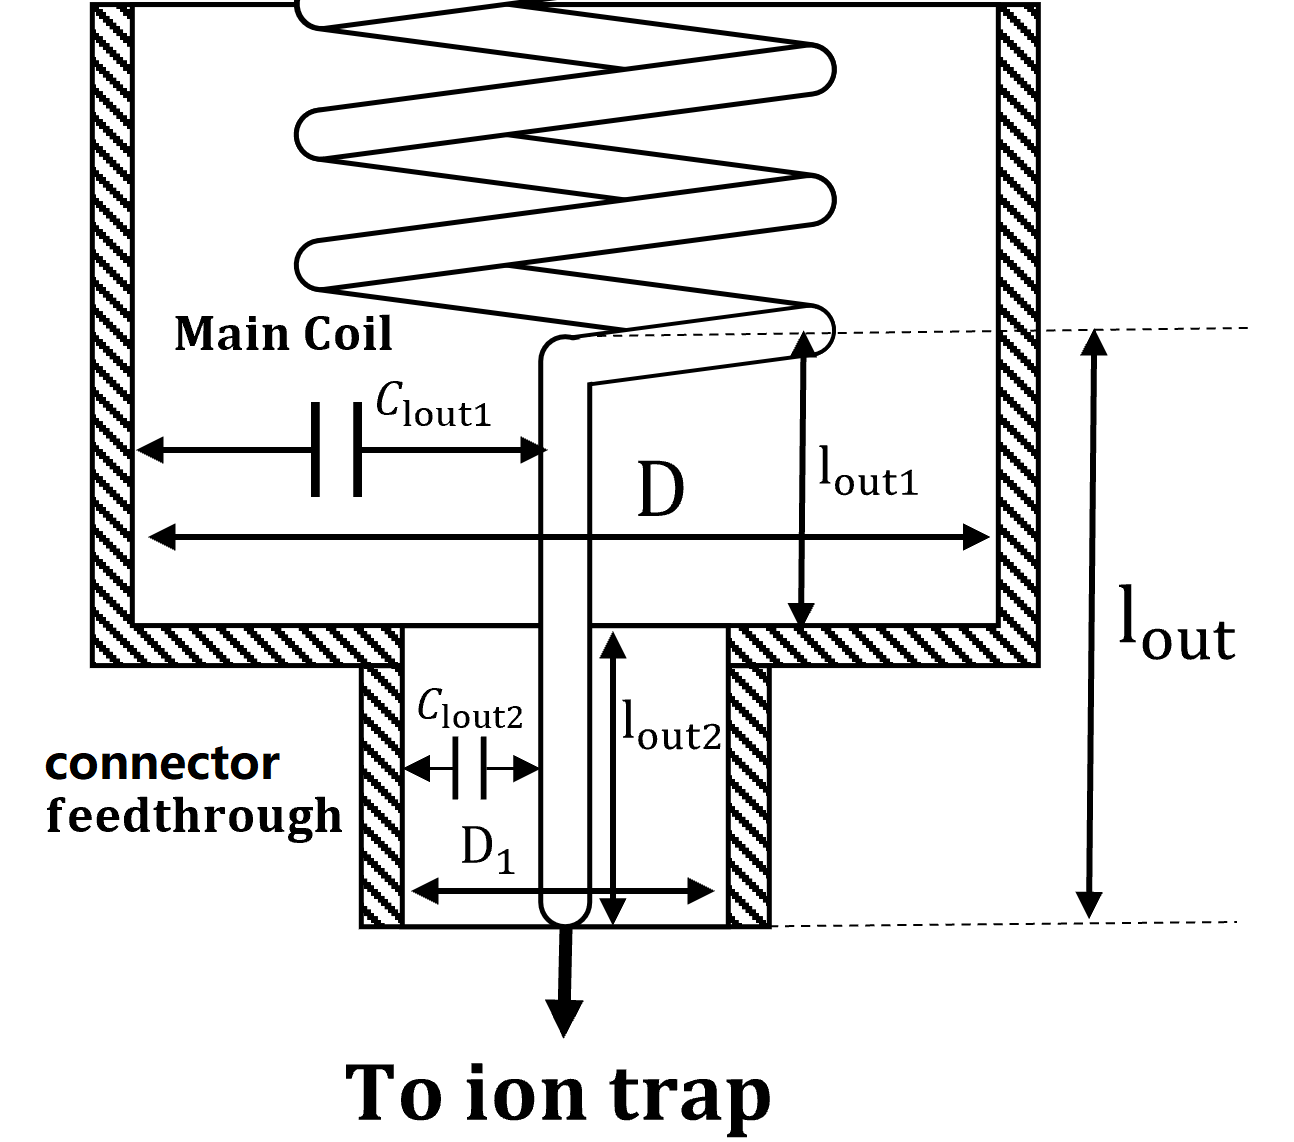
\includegraphics[width=0.5\linewidth]{helical/helical_lout_2}
\end{figure}

仿真结果如图\ref{fig:helical_lout_1}所示。随着输出导线长度的增加,谐振频率下降。$Q$随着谐振频率的减小而减小,两者成正比,与公式\eqref{eq:helical_Q_equation}具有相同的关系。这主要是输出线引入额外电容而对电阻和电感影响较小导致的。

\begin{figure}
    \centering
    \caption[输出线部分影响]{输出线部分影响。横坐标为输出线长$l_{out}$(单位mm),蓝色‘*’标和‘+’标分别为仿真和实验的频率$F$(单位MHz,对应左侧纵坐标),橙色‘o’标和‘x’标分别为仿真和实验的品质因子$Q$(单位1,对应右侧纵坐标)。\label{fig:helical_lout_1}}
    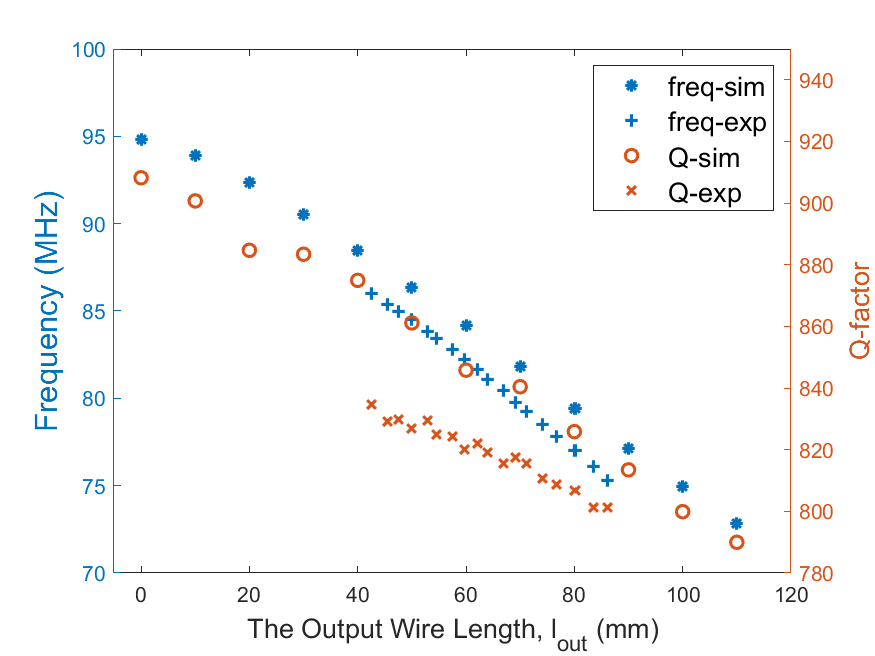
\includegraphics[width=0.8\linewidth]{helical/helical_lout_1}
\end{figure}

为了验证仿真结果,我们进行了输出导线长度切割实验,测量了输出导线长度和器件谐振频率$f_0$和$Q$。结果如图\ref{fig:helical_lout_1}所示。实验与模拟的频率差约为$2$MHz,实验测量的$Q$数据比模拟低约$150$。为了在同一图中绘制$ Q $数据,实验$ Q $数据偏移了$ 100$。除了偏移之外,频率$f_0$和$ Q $都与其对应的数据一致。该结果再次表明了仿真结果的可信度。

文献\cite[]{Gandolfi_Niedermayr_Kumph_Brownnutt_Blatt_2012,Macalpine_Schildknecht_1959, Deng_Sun_Yuan_Xu_Zhang_Lu_Luo_2014}之前研究中的理论预测和实验之间的大频率误差可能来自于忽略输出线电容\cite[]{Nandi_Sikdar_Das_Ray_2022, Batra_Panja_De_Roy_Majhi_Yadav_Sen_Gupta_2017}。我们给出了改进的LCR电路模型和一种新的电容评估公式来估计频率。与 HFSS 仿真结果相比,我们的新模型的频率预测有了很大的提高,更多细节见第\ref{section:helical_theory_model}节。

\subsection[屏蔽外壳参数的影响]{屏蔽外壳参数的影响}
\begin{figure}
    \centering
    \caption[屏蔽外壳的影响]{屏蔽外壳的影响,横坐标为屏蔽壳内直径$D$(单位mm),纵坐标为频率$F$(单位MHz)。蓝色实线和‘*’标点为频率(单位MHz,对应左侧纵坐标),橙色虚线和‘o’标点为品质因子Q(单位1,对应右侧纵坐标)。\label{fig:helical_shield_diameter}}
    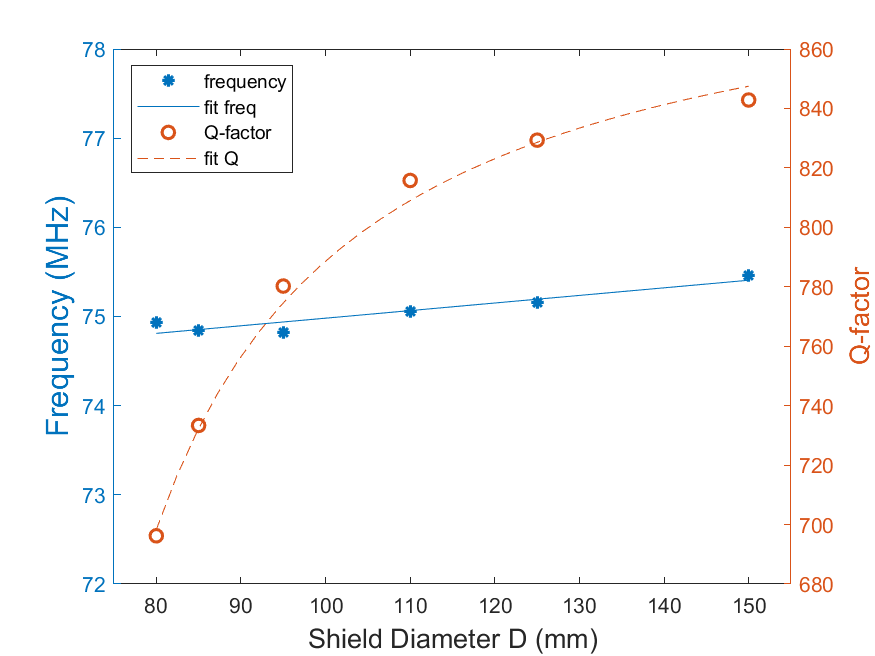
\includegraphics[width=0.8\linewidth]{helical/helical_shield_diameter}
\end{figure}

铜屏蔽外壳完成了电流回路,定义了螺旋谐振腔中的EM场边界条件。屏蔽外壳和主线圈形成电容$C_s$,因此屏蔽的直径对谐振频率有影响。屏蔽外壳可以屏蔽和减少电磁场辐射耗散,因此谐振器将具有高$Q$因子。在这里,通过数值模拟研究了屏蔽外壳直径$ D $对频率$f_0$和$ Q $因子的影响。结果如图\ref{fig:helical_shield_diameter}所示,当屏蔽直径$ D $增加时,频率$f_0$和$ Q $因子都会增加。频率变化很小,而$ Q $因子首先快速增长,然后逐渐减慢。频率的微弱增加是由于侧壁电容随着屏蔽外壳$D$的增大而减小。$Q$因子的增加是因为屏蔽直径越大,电场强度越小,屏蔽电流越小,电阻相等,耗散越小。因此为了获得更大的$Q$,在合理的设备尺寸下将首选较大的屏蔽直径。

屏蔽外壳高度的影响与相对于外壳沿轴向移动主线圈位置并相应地调整端帽位置相同。结果如图\ref{fig:helical_bias_axial}所示。屏蔽高度对频率$f_0$和$Q$因子的影响很小。

\subsection[耦合线圈参数的影响]{耦合线圈参数的影响}

耦合线圈是螺线管谐振腔的一个有趣部分。通过调节耦合线圈的形状和位置可以满足阻抗匹配工作,实现最佳耦合以最小化散射参数$S_{11}$。然而,据我们所知,以前还没有耦合线圈几何形状影响的具体相关研究。在这里,数值模拟方法提供了研究这些问题的机会。

\begin{figure}
    \centering
    \caption[耦合线圈的影响]{耦合线圈的影响。$\Delta h$:耦合线圈和主线圈之间的距离(单位mm);$d$:耦合线圈的直径(单位mm);$\tau$:耦合线圈的螺距(单位mm)。\label{fig:helical_primary_coil}}
    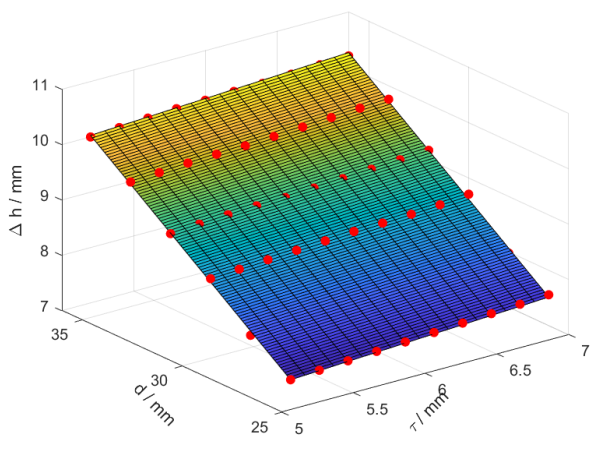
\includegraphics[width=0.8\linewidth]{helical/helical_primary_coil}
\end{figure}

为了研究主线圈形状效应,我们在其他参数满足表\ref{tb:helical_simulation_parameters}中第9行的情况下,模拟了各种耦合线圈尺寸(耦合线圈直径$d_1$和螺距$\tau_1$)及其轴向位置,并试图满足阻抗匹配。
对于每个耦合线圈(直径$d_1$和螺距$\tau_1$),扫描和优化耦合线圈在轴向的位置,以实现最小耦合反射$S_{11}$。
如果$S_{11}$系数可以达到$-45$dB或更低,认为阻抗匹配过程完成,同时记录耦合线圈轴向位置。仿真结果如图\ref{fig:helical_primary_coil}所示。
$x$轴和$y$轴分别为直径$d_1$和俯仰$\tau_1$,$z$轴为耦合线圈达到最佳耦合条件时的轴向位置。
结果表明,所有$ d_1,\ \tau_1 $参数设置都具有最佳的耦合位置$ \delta_1$,几乎所有数据点($d_1,\tau_1\delta_1$)都位于同一平面表面上。
这意味着耦合线圈的绝对形状对于实现阻抗匹配过程并不重要。在合理范围内,总可以通过调整耦合线圈轴向位置来补偿耦合线圈的所有变形。

\section{谐振腔耦合过程特性}
谐振腔的实际使用离不开一个十分重要的过程,即阻抗匹配,我们一般称为耦合。经验上来看,我们知道可以通过移动耦合线圈和主线圈之间的距离或者改变耦合线圈的形状来实现耦合。一般来说实践上我们更倾向于改变耦合线圈和主线圈之间的距离的方式来实现耦合,存在一个最优距离使得匹配最佳,两者的距离太近或者太远都无法实现最佳匹配。只有在最佳匹配的时候微波功率透过谐振腔的传输率才能达到最大。在耦合的过程中谐振腔的最佳耦合频率会发生微小的偏移,而Q值则会发生较大的变化。值得注意的是,我们发现耦合过程中最佳耦合频率点和Q值的变化并不像最佳耦合点一样有最有值,如图\ref{fig:helical_coupling_delta}所示,它们是随着耦合距离单调变化的。也就是说,在最佳耦合点左右两侧,虽然透过率都会下降,但是两侧的Q值却是大不相同的。从图\ref{fig:helical_coupling_delta}中可见最佳匹配点左右两侧的Q值差能达到一倍之多,这给我们带来的启示是:我们可以通过牺牲一定的微波功率透过率来获得更高的Q值或者相反。
\begin{figure}
    \centering
    \caption[谐振腔耦合过程特性]{谐振腔耦合过程特性。横坐标为耦合线圈到主线圈的距离$\Delta h$,左侧和右侧的纵坐标分别是品质因子数值(单位1)和散射系数值(单位dB)。其中蓝色‘o’标线是谐振腔的品质因子Q,红色‘*’标线是相应的最佳耦合时的反射系数最小值$S_{11}^{min}$,绿色‘o’标线是相应的最佳耦合时的透射系数最大值$S_{21}^{max}$。\label{fig:helical_coupling_delta}}
    \includegraphics[width=0.8\linewidth]{helical/helical_coupling_delta}
\end{figure}

从上面的耦合过程结果来看,耦合线圈距离主线圈距离越远的情况下Q值越高。也就是说两者相互‘影响’越小的情况下Q值会越高。这个影响实际上就是等效的阻抗带来的耗散,为了验证这一点我们进行了另一组仅改变耦合线圈电阻值的实验,结果如图\ref{fig:helical_coupling_rin}所示。从图\ref{fig:helical_coupling_rin}中可以看出,随着耦合线圈电阻值的增加,Q值逐渐下降,同时也伴随着最佳耦合频率的偏移。不难发现,增加耦合线圈电阻值的过程这个结果跟图\ref{fig:helical_coupling_delta}中耦合线圈与主线圈距离的减小过程的结果是相互对应的。
\begin{figure}
    \centering
    \caption[谐振腔耦合过程特性]{谐振腔耦合过程特性。横坐标为耦合线圈的阻值$R$,左侧和右侧的纵坐标分别是品质因子数值(单位1)和散射系数值(单位dB)。其中蓝色‘o’标线是谐振腔的品质因子Q,红色‘*’标线是相应的最佳耦合时的反射系数最小值$S_{11}^{min}$,绿色‘o’标线是相应的最佳耦合时的透射系数最大值$S_{21}^{max}$。\label{fig:helical_coupling_rin}}
    \includegraphics[width=0.8\linewidth]{helical/helical_coupling_rin}
\end{figure}


% \textcolor{red}{可以考虑将耦合过程会有不同的Q值的那个图也放上来说明一下\dots}

\newpage
\section[螺线管谐振腔的数学建模]{螺线管谐振腔的数学建模\label{section:helical_theory_model}}

螺线管谐振腔的集总电路模型可以解释和预测器件的行为。一个好的电路模型可以帮助研究人员轻松地设计具有特定属性的设备。在这里,对于螺线管谐振腔,谐振频率和较高的Q因子是最重要的两个指标。首先,对于谐振频率,我们假设额外的输出导线长度电容是频率误差发生的主要原因,如第\ref{section:helical_output_wire}节所述。

\begin{figure}
    \centering
    \caption[LCR电路模型]{LCR电路模型。$L$表示谐振腔的电感,主要包括耦合线圈和主线圈的电感;$R$表示整个谐振腔的电阻;$C$表示谐振腔的电容,$C_x$表示谐振腔内部结构的电容,$C_{lout}$表示谐振腔输出线引入的电容。\label{fig:helical_RLC_circuit1}}
    \includegraphics[width=0.8\linewidth]{helical/helical_RLC_circuit1}
\end{figure}

因此,输出线电容被添加到LCR电路模型中,如图\ref{fig:helical_RLC_circuit1}所示。总等效电容可视为传统电容CT和输出线总电容$C_{lout}$的总。传统的电容部分与以往的研究相同,而输出线和外部屏蔽将形成同轴电容:
\begin{align} 
	C_{lout}&=C_{lout1}+C_{lout2} \label{eq:helical_lout}\\ 
	C_{lout1}&=\frac{2\pi\epsilon_0 l_{out1}}{ln(D/d_0)} \label{eq:helical_lout1}\\ 
	C_{lout2}&=\frac{2\pi\epsilon_0 l_{out2}}{ln(D_1/d_0)} \label{eq:helical_lout2}
\end{align}

其中输出线电容$C_{lout1}$($C_{lout2}$)是长度为$l_{out1}$($l_{out2}$)的输出线与内径为$D$($D_1$)侧壁形成的电容。

然而,在补偿输出线长效应后,频率预测仍然低于数值模拟或实验结果。经过多次尝试,我们发现主要原因是对电容$C_c$和$C_s$的高估。最近的一项研究\cite[p52,f5.3]{article_2010}给出了一个螺线管电容$C_c$的新估计公式:
\begin{align}
    C_c=\frac{4\epsilon_0 b}{\pi}(1+k_c)/cos^2\psi 	\label{eq:helical_C_c_new}
\end{align}

其中$k_c=0.717439(d/b)+0.933048(d/b)^{3/2}+0.106(d/b)^2$,$d$是螺线管的直径,$b$是螺线管的长度,$\psi$是螺距角($\tan\psi=\tau/(\pi d)\approx 1$),$\epsilon_0$是真空介电常数。

另一方面,屏蔽壁电容$C_s$在主线圈和外部屏蔽壁之间形成,与电容$C_{lout}$相同,因此同轴电容公式可用于计算$C_s$。主线圈的等效同轴线长度为$Nd_0$,单匝等效长度为$d_0$,总主线圈有$N$匝,因此屏蔽电容计算为:
\begin{align}
    C_s=2\pi\epsilon_0 \frac{Nd_0}{ln(D/d')} \label{eq:helical_C_s_new}
\end{align}

其中$d'$是一个等效的线圈直径,$d'=d+\pi d_0/4$,其中$\pi d_0/4$是一个用于修正线圈边缘效应的因子。

此外,实际的主线圈螺旋长度有限,匝稀疏,因此需要更新或修改文献\cite[]{Siverns_Simkins_Weidt_Hensinger_2012}中的电感计算方法。短螺旋电感估计方法可计算为:
\begin{align}
    L=\frac{\mu_0 \pi (d/2)^2 }{\tau^2} (\sqrt{b^2+(d/2)^2}-d/2) \label{eq:helical_L_new}
\end{align}

\begin{figure}
    \centering
    \caption[三种理论模型的预测效果比较]{三种理论模型的预测效果比较。左、中、右图分别是30MHz、50MHz、75MHz附近频率设置的模型与参考表中偏差的结果的频数统计图。作为参考,每幅图上方给出了所有偏差的均值和其标准差。\label{fig:helical_freqmodelcompare}}
    \subcaptionbox[HUST模型结果]{HUST模型结果\label{fig:helical_freqmodelcompare_hust}}{
        \includegraphics[width=0.55\linewidth]{helical/helical_freqmodelcompare_hust}
    }
    \subcaptionbox[Sussex模型结果]{Sussex模型结果\label{fig:helical_freqmodelcompare_sussex}}{
        \includegraphics[width=0.55\linewidth]{helical/helical_freqmodelcompare_sussex}
    }
    \subcaptionbox[SUST模型结果]{SUST模型结果\label{fig:helical_freqmodelcompare_sust}}{
        \includegraphics[width=0.55\linewidth]{helical/helical_freqmodelcompare_sust}
    }

\end{figure}

最后,我们通过更新上述所有估计的方法,得到了一个新的频率预测模型。我们比较了频率预测模型、Sussex模型\cite[]{Siverns_Simkins_Weidt_Hensinger_2012}、SUST模型(本文)和 HUST模型\cite[]{Deng_Sun_Yuan_Xu_Zhang_Lu_Luo_2014}的准确性。
基于数值模拟结果,通过统计直方图对模型的有效性和准确性进行比较和评估,如图14(c)所示。频率误差的平均值和标准差越小,精度越好,误差离散越小。
所有的模型都与仿真的结果为标准做比较。
图\ref{fig:helical_freqmodelcompare}中的每一个数据结果都是一些列可行的$d,\tau$参数组合的模型预测和仿真结果的差值$\delta f=f_{model}-f_{HFSS}$,最终绘制出误差的统计分布。
针对不同的谐振频率组计算和模拟一系列离散的$d,\tau$参数(与表\ref{tb:helical_simulation_parameters}$30$MHz、$50$MHz、$75$MHz)。$d$的样本在$20-80$mm的范围内,步长为$10$mm;$\tau$的样本在$4-18$mm的范围内,步长为$2$mm。
平均偏差和标准偏差都在每个图的顶部标记。平均值是一个有符号值,表示模型的整体频率预测效果。标准差表示频率误差的离散程度。


% \begin{figure}
%     \centering
%     \caption[HUST模型结果]{HUST模型结果\label{fig:helical_freqmodelcompare_hust}}
%     \includegraphics[width=0.33\linewidth]{helical/helical_freqmodelcompare_hust}
% \end{figure}

% \begin{figure}
%     \centering
%     \caption[Sussex模型结果]{Sussex模型结果\label{fig:helical_freqmodelcompare_sussex}}
%     \includegraphics[width=0.33\linewidth]{helical/helical_freqmodelcompare_sussex}
% \end{figure}

% \begin{figure}
%     \centering
%     \caption[SUST模型结果]{SUST模型结果\label{fig:helical_freqmodelcompare_sust}}
%     \includegraphics[width=0.33\linewidth]{helical/helical_freqmodelcompare_sust}
% \end{figure}

直方图结果表明:对于$75$MHz组,本文中的模型的均值和标准差(SUST)在三个模型中都是最小的,预测的准确性是最好的。对于 $50$MHz组,SUST和HUST模型之间的平均偏差值和标准偏差值基本相似。它们都预测了比Sussex模型更准确的谐振频率。对于$30$MHz组,HUST频率预测的平均值最小,SUST模型准确率次之,但它们都优于Sussex模型。HUST和SUST模型的标准偏差相似,但它们都优于Sussex模型。需要注意的是,在30MHz组中,由于主线圈线长度约束,所有$56$种可能组合中只有$11$个可行数据,参见公式\eqref{eq:helical_fixed_constraints_1}和\eqref{eq:helical_fixed_constraints_2},因此结果可能会波动和偏差很大。

在上述结果中,对于$30-80$MHz频率范围内的情况,本文提出的LCR模型提高了预测精度。输出线效应(参见第\ref{section:helical_output_wire}节)作为对分布式电容效应的替代解释,给出了更简单直观的物理解释。

\section[螺线管谐振腔的机械结构优化]{螺线管谐振腔的机械结构优化}

\subsection[惯用旧版谐振腔]{惯用旧版谐振腔}
惯用的旧版谐振腔设计如图\ref{fig:helical_old_design}所示。在该设计中,主线圈的接地/直流输入端口安装在谐振腔侧壁、即主屏蔽壳上。在采用以SMA为代表的射频连接头作为端口时,会产生额外的径向长度,导致配件之间的机械冲突,安装的时候主线圈很难直接放入外筒中。装配时一般需要先将输出头向内弯折,进入筒后再进行折回,将射频接头上紧固定;或者先将射频头固定在侧壁上,装入主线圈后再进行焊接。上述两种安装方式都缺乏便利性,比如弯折过程中射频连接头焊接会脱落、或壳内焊接的复杂度较高。更重要的是,安装时往往会破坏主线圈的结构,很难完全恢复到进筒前的结构参数。还有,该设计中对主线圈的支持较弱,主线圈易形变。这在装配时会导致难以将线圈按照目标设计参数准确地进行装配,增加调试成本。即使装配好了,在工作过程中也会对外界机械抖动等较为敏感、稳定性差。该设计的耦合方式也就奥维笨拙,在实际使用中需要华为大量时间来拆卸谐振腔、调整腔内小线圈的形状来实现最佳耦合。
除此之外,该设计的主线圈输出端口的便利性、稳定性以及屏蔽性能较差。为了减小金属电容板与线圈之间的等效电容影响,通孔直径较大,使得谐振腔的信号泄露增加、屏蔽效果减弱。而谐振腔在与后级设备进行连接时,通过中空螺柱进行压接连接,稳定性较差。
为此,我们设计了一款新的谐振腔来解决以上提到的一些问题。

\begin{figure}
    \centering
    \caption[旧版的谐振腔设计]{旧版的谐振腔设计,有机械冲突、耦合方式较差。\label{fig:helical_old_design}}
    \includegraphics[width=1.0\linewidth]{helical/helical_old_design}
\end{figure}
\subsection[易装配易耦合的新版谐振腔]{易装配易耦合的新版谐振腔}
新的易装配易耦合的模块化谐振腔设计如图\ref{fig:helical_new_design}所示。它解决了现有技术对主线圈的安装较为不便、对主线圈固定的稳定性差、对次级线圈耦合部分缺乏灵活调节的问题。新的设计主要包括以下结构:
\begin{enumerate}
    \item 主腔体屏蔽与支撑部分,包括:主屏蔽壳、底部和顶部两个固定板(记为固定板一与固定板二)、四个固定柱、一个输出屏蔽壳;
    \item 线圈及其固定与调节结构,包括:一个或两个主线圈(以下图示说明均使用两个主线圈情况、但本结构同样适用于一个主线圈的情况)、一对主线圈固定支架、一个次级线圈、一个非旋转伸缩套筒、一个射频分压电路模块;
    \item 电学相关接口与紧固零件,包括:射频输入与输出接头、直流输入接头、射频分压输出接头、及若干固定螺丝。
\end{enumerate}

新设计的实物图如图\ref{fig:helical_new_design_real}所示,将主线圈的接地/直流输入端口转移至底部固定板一。安装时可以直接固定好底座,然后将主屏蔽壳套上,再盖上顶部的固定板,最后用四个固定柱将上下两个固定板连接起来即可。安装过程不存在装配上的机械冲突。
新设计采用一对主线圈固定支架对主线圈进行支撑与固定,通过固定支架上面的凹槽设计来约束线圈为目标参数(螺线的直径、螺距、长度)。这样在装配时易按照设计目标参数进行装配,在使用过程中也能够保持稳定。
新设计巧妙地采用了非旋转伸缩套筒来实现小线圈的平动耦合。非旋转伸缩套筒可实现高精度的平动,常用于光学系统中透镜的高精度调节。套筒中心可以用来固定射频接头,并与次级线圈连接,方便次级线圈的固定和外部信号输入。非旋转伸缩套筒的表面可以镀上氧化层,形成次级线圈部分与其它部分的绝缘,很好地隔离了两者,保证了次级线圈与主线圈仅通过自由空间进行耦合,接地部分不会相互干扰。
本设计通过主线圈末端焊接射频连接头、并固定至顶部固定板,来实现谐振腔的输出。该设计中,谐振腔主腔体几乎完全封闭,增加屏蔽效果,减少腔内信号泄露、以及腔外噪声的耦入。输出为标准射频接口,与后级设备连接的便利性更高,且稳定性也有了进一步的提升。

与现有技术相比,本设计设计更为合理,元件装配更加方便,谐振耦合更加精细快捷,谐振腔长时工作的稳定性更高。
\begin{figure}
    \centering
    \caption[易装配易耦合的谐振腔设计]{易装配易耦合的谐振腔设计\label{fig:helical_new_design}}
    \includegraphics[width=1.0\linewidth]{helical/helical_new_design}
\end{figure}

\begin{figure}
    \centering
    \caption[易装配易耦合的谐振腔设计实物图]{易装配易耦合的谐振腔设计实物图\label{fig:helical_new_design_real}}
    \includegraphics[width=1.0\linewidth]{helical/helical_new_design_real}
\end{figure}







\newpage
\section[章末小结]{章末小结}
螺线管谐振腔是离子阱系统中一种重要的测控器件,用于产生囚禁离子的微波信号。本章使用有限元(FE)仿真及实验相结合的方式研究了离子阱量子系统中的螺线管谐振腔。首先介绍了螺线管谐振腔在离子阱系统中的重要作用以及现有谐振腔设计的方式的问题和局限。接着使用商业有限元仿真软件HFSS建立了螺线管谐振腔的仿真模型,并且实际制作了若干组谐振腔进行了测试,通过将仿真结果与实验结果对比的方式验证了仿真模型的正确性和准确性。这一结果为谐振腔的进一步研究做好了准备,通过仿真预研的方式可以及大地方便对谐振腔各类物理参数变化的研究过程并且降低了研究成本。

Q值是谐振腔在离子阱量子计算系统中应用时关注的核心指标,更高的Q值能够带来更稳定的离子囚禁以及更高的离子比特保真度。本章接着针对适用于离子阱的特定频率范围的谐振腔Q值进行了优化研究,使用FE仿真的方式以紫铜材料为基础对谐振腔的各类几何结构参数变动对Q值和频率的影响进行了具体研究和分析。结果表明了主线圈的几何参数尤其是其直径、螺距和总线长是谐振腔性能最主要的影响因素。通过对谐振腔耦合过程特性的分析得出了用于耦合的小线圈几何参数对最佳耦合下的频率和Q值结果几乎没有影响,我们应将更多精力放在主线圈的设计和准确实现上。我们也从优化结果中找到了一组最优的几何参数进行了制作和测试并将其应用到了组内的离子阱实验系统中。

通过对螺线管谐振腔的仿真及实验数据结果的处理以及对谐振腔几何结构的分析,本章引入一种改进的LCR电路模型和新的电容评估公式给出了一个更加物理化的谐振腔频率计算数学模型。相较于HUST和Sussex的数学模型结果,本章所给出的方法在多个频率段都有着更高的准确性。尽管通过数学模型计算得到的谐振腔频率与实际制作结果仍然存在差距,但是这种方式可以帮助研究者快速锁定大致几何参数范围,以更加高效快捷地使用仿真工具进行优化设计。
除此之外,对于实验系统中的谐振腔装配结构也进行了优化设计,给出了一种装配和耦合更方便且更加稳定的模块化谐振腔设计并制作和应用到了实验系统中,极大地促进了离子阱量子计算实验系统的稳定度和集成化。
% !TeX root = ../sustechthesis-example.tex


\chapter[RTMQ测控系统应用:离子阱频率、激光功率和激光拍频稳定]{RTMQ量子测控系统应用:离子阱频率、激光功率和激光拍频稳定\label{section:implementation}}

% 值得注意的是,RTMQ量子测控系统不仅可以完成常规的量子物理实验实时控制的需求,同时还可以不受影响地执行一些量子计算系统的实验背景环境维护这些实验背景环境原来常常需要一大堆模拟PID控制器、滤波器、放大器等等来进行建构和实现。RTMQ系统凭借其数字化的优势而可以及大地简化整个实验平台仪器的使用,使实验过程有着更强的可控性和更好的自动化水平。

% 本章将通过介绍使用RTMQ量子测控系统构建离子量子计算系统中几个重要子系统来进一步展示该系统的集成性和易用性。
量子测控系统说到底是要为量子物理实验服务的,量子计算最关注的基础指标之一就是量子操作的保真度。对于离子量子计算来说,影响其保真度的主要因素是系统中的射频和激光信号的稳定性。因而,测控系统最基本的任务便是通过各种控制回路为离子量子计算系统构建稳定的射频和激光。
此外,任何测控系统的使用也都必须落地到实际的软硬件上。测控系统硬件的设计除了需要考虑所采用的系统架构外,还需要根据具体的实验需求整合各种功能器件以及拓展一些板上的功能性软固件。

基于对离子量子计算(第\ref{section:quantum_computation}章)和RTMQ测控架构(第\ref{section:fpga_rtmq}章)内容的理解和拓展,本章将首先介绍量子操作的保真度,接着给出基于RTMQ架构的量子测控系统测控板的设计,包括测控板硬件设计架构、芯片选型、重要系统功能外设及其FPGA实现等。在此基础上结合螺线管谐振腔(第\ref{section:helical}章)、激光器等器件搭建和测试离子阱频率稳定、激光功率稳定和激光拍频稳定等几个离子阱量子计算提高保真度相关的重要子系统,过程中也给出RTMQ系统的两个重要功能外设拓展——高速通用数字PID和高速通用数字IIR滤波器的设计及FPGA实现。
% 此外,该套RTMQ量子测控系统在有关比特控制和量子模拟策略等的相关内容的量子实验上的应用可以在参见我们实验室过去发表的文章\cite[]{Zhang_Wang_Wang_Zhang_Wu_Jie_Lu_2022}。






\section[量子比特操作的保真度]{量子比特操作的保真度}
% ============================================================================
% ============================================================================
% =======================    量子比特操作的保真  ===============================
% ============================================================================
% ============================================================================


量子比特操作的保真度是量子计算研究过程中十分关注的指标,J.P.G. van Dijk等人\cite[]{van_Dijk_Kawakami_Schouten_Veldhorst_Vandersypen_Babaie_Charbon_Sebastiano_2019}详细的分析了经典电子学控制操作对量子比特保真度的影响。对量子比特进行的操作可以用一个时变的哈密顿量$H(t)$来描述,它可以被近似表述为一系列时不变的组成:
\begin{align}
    U\approx \prod_{n=N}^{0} e^{-iH(n\Delta t)\Delta t}
\end{align}

其中$\Delta t$是时间步长,它比需足够小以达到良好的近似。而操作的保真度即这个实际的操作$U$与理想操作$U_{ideal}$之间的近似度,对$n$维希尔伯特空间的操作保真度$F$计算如下:
\begin{align}
    F=\frac{1}{n^2}\left|Tr\left[U_{ideal}^{\dagger}U\right]\right|^2
\end{align}

% 单比特操作的希尔伯特空间$n=2$,两比特操作的希尔伯特空间$n=4$,以此类推,$N$比特门的希尔伯特空间将为$n=2^N$。可见随着量子比特数量的增加其整体操作的保真度会以$\frac{1}{n^2}$的速度急剧下降,因而大规模量子计算机的实现必须要不断提高量子比特操作的保真度。



% \begin{table}
%     \centering
%     \caption[电子学控制信号误差和噪声影响下的单比特操作保真度]{电子学控制信号误差和噪声影响下的单比特操作保真度\cite[]{van_Dijk_Kawakami_Schouten_Veldhorst_Vandersypen_Babaie_Charbon_Sebastiano_2019}。其中,$\theta$是目标的操作旋转角度,范围从$-\pi$到$\pi$;信号误差记为$\Delta$;$S_(\omega)$为噪声能量谱密度(PSDs);$H_(\omega)$为量子比特的传递函数;$\omega_{min}$为积分底限。\label{tb:fidelity}}    
%     \begin{tabular}{L{2cm}L{5.5cm}L{5.5cm}}
%         \toprule
%         & 误差 & 噪声 \\
%         \midrule
%         \multicolumn{3}{c}{载波}\\
%         % \hline
%         频率 & $1-\frac{1}{2}\left[1-cos{\theta}\right]\left(\frac{\Delta \omega_{mw}}{\omega_R}\right)^2$ & $1-\frac{1}{\pi}\int_{\omega_{min}}^{\infty}\frac{S_{mw}(\omega)}{\omega_R^2}\left|H_{mw}(\omega)\right|^2 d\omega$ \\
%         相位 & $1-\frac{1}{2}\left[1-cos{\theta}\right]\Delta \phi^2$ & \\
%         \hline
%         \multicolumn{3}{c}{波包}\\
%         % \hline
%         幅度 & $1-\frac{1}{4}\theta^2\left(\frac{\Delta\omega_R}{\omega_R}\right)^2$ & $1-\frac{1}{\pi}\int_{\omega_{min}}^{\infty}\frac{S_{R}(\omega)}{\omega_R^2}\left|H_{R}(\omega)\right|^2 d\omega$ \\
%         时间长度 & $1-\frac{1}{4}\theta^2\left(\frac{\Delta T}{T}\right)^2$ & $1-\frac{1}{\pi}\int_{\omega_{min}}^{\infty}S_{\phi}(\omega)\left|H_{T}(\omega)\right|^2 d\omega$ \\
%         \bottomrule
%     \end{tabular}
% \end{table}

% \begin{table}
%     \centering
%     \caption[电子学控制信号误差和高斯噪声影响下的单比特操作保真度]{电子学控制信号误差和高斯噪声影响下的单比特操作保真度\cite[]{van_Dijk_Kawakami_Schouten_Veldhorst_Vandersypen_Babaie_Charbon_Sebastiano_2019}。其中,$\theta$是目标的操作旋转角度,范围从$-\pi$到$\pi$;信号误差记为$\Delta$;$S_{\omega}$为噪声能量谱密度(PSDs);$H_{\omega}$为量子比特的传递函数;$\omega_{min}$为积分底限。\label{tb:fidelity}}    
%     \begin{tabular}{L{1.5cm}L{6cm}L{6cm}}
%         \toprule
%         & 误差 & 高斯噪声 \\
%         \midrule
%         \multicolumn{3}{c}{载波}\\
%         频率 & $1-\frac{1-cos{\theta}}{2}\alpha^2,\alpha=\frac{\Delta \omega_{mw}}{\omega_R}$ & $1-\frac{1}{\pi}\int_{\omega_{min}}^{\infty}\frac{S_{mw}(\omega)}{\omega_R^2}\left|H_{mw}(\omega)\right|^2 d\omega$ \\
%         相位 & $1-\frac{1-cos{\theta}}{2}\alpha^2,\alpha=\Delta \phi$ & \\
%         % 附加 &  & $1-\frac{1}{\pi}\int_{\omega_{min}}^{\infty}\frac{S_{add}(\omega-\omega_0)}{\omega_R^2}\left|H_{add}(\omega)\right|^2 d\omega$ \\
%         \hline
%         \multicolumn{3}{c}{波包}\\
%         幅度 & $1-\frac{1}{4}\theta^2\alpha^2,\alpha=\frac{\Delta\omega_R}{\omega_R}$ & $1-\frac{1}{\pi}\int_{\omega_{min}}^{\infty}\frac{S_{R}(\omega)}{\omega_R^2}\left|H_{R}(\omega)\right|^2 d\omega$ \\
%         时长 & $1-\frac{1}{4}\theta^2\alpha^2,\alpha=\frac{\Delta T}{T}$ & $1-\frac{1}{\pi}\int_{\omega_{min}}^{\infty}S_{\phi}(\omega)\left|H_{T}(\omega)\right|^2 d\omega$ \\
%         \bottomrule
%     \end{tabular}
% \end{table}

在实验中进行量子比特操作时,具体参数的设置误差、环境中存在的背景噪声、来自操作信号自身的噪声和抖动以及不同量子比特操作时的相互串扰噪声都会导致保真度的降低。
具体参数的设置有赖于实验人员的尝试和优化,而背景噪声和串扰噪声的解决有赖于背景环境和比特操作策略的系统设计,测控系统需要解决的问题是整个量子计算系统中涉及到的信号自身噪声和抖动,比如射频和激光信号的频率、幅度、相位稳定性等。

\begin{table}
    \centering
    \caption[操作信号微小误差和高斯噪声影响下的单比特操作保真度]{操作信号微小误差和高斯噪声影响下的单比特操作保真度$\theta$是操作的目标旋转角度,范围从$-\pi$到$\pi$;信号误差记为$\Delta$;$S(\omega)$为噪声能量谱密度(PSDs);$H(\omega)$为量子比特的传递函数;$\omega_{min}$为积分底限。\label{tb:fidelity}}    
    \begin{tabular}{L{1.5cm}L{5cm}L{7cm}}
        \toprule
        & 误差 & 高斯噪声 \\
        \midrule
        \multicolumn{3}{c}{载波}\\
        频率 & $1-\frac{1-cos{\theta}}{2}\alpha^2,\alpha=\frac{\Delta \omega_{mw}}{\omega_R}$ & $\frac{1}{2}\left(1+e^{-2\alpha^2}\right) sin^4\left(\frac{\theta}{2}\right)+cos^4\left(\frac{\theta}{2}\right)+\frac{1}{2} e^{-\frac{\alpha^2}{2}} sin^2\left(\theta\right), \alpha=\frac{\sigma_{\omega_{mw}}}{\omega_R}$ \\
        相位 & $1-\frac{1-cos{\theta}}{2}\alpha^2,\alpha=\Delta \phi$ & $\frac{1}{2}\left(1+e^{-2\alpha^2}\right) sin^4\left(\frac{\theta}{2}\right)+cos^4\left(\frac{\theta}{2}\right)+\frac{1}{2} e^{-\frac{\alpha^2}{2}} sin^2\left(\theta\right), \alpha=\sigma_{\phi}$ \\
        \hline
        \multicolumn{3}{c}{波包}\\
        幅度 & $1-\frac{1}{4}\theta^2\alpha^2,\alpha=\frac{\Delta\omega_R}{\omega_R}$ & $\frac{1}{2}+\frac{1}{2} e^{-\frac{1}{2}\alpha^2\theta^2},\alpha=\frac{\sigma_{\omega_R}}{\omega_{R,ideal}}$ \\
        时长 & $1-\frac{1}{4}\theta^2\alpha^2,\alpha=\frac{\Delta T}{T}$ & $\frac{1}{2}+\frac{1}{2} e^{-\frac{1}{2}\alpha^2\theta^2}, \alpha=\frac{\sigma_T}{T_{ideal}}$ \\
        \bottomrule
    \end{tabular}
\end{table}

信号本身导致的保真度降低的因素主要有两类,一类是信号设置的绝对误差,另一类是信号自身的噪声。常见的噪声一般都近似为高斯分布,以激光对离子量子比特的单比特操作为例,表\ref{tb:fidelity}中给出了若干操作信号微小误差和高斯噪声影响下的单比特操作保真度计算方法。表中的计算基于较高保真度情况下的结果,也即涉及到的各类误差都为微小误差,且对于频率误差和噪声不考虑其与离子相互作用的响应情况。

激光信号自身频率误差和相位误差影响下忽略高阶项后的保真度计算为:
\begin{align}
    F\approx1-\frac{1-cos{\theta}}{2}\alpha^2+\mathcal{O}\left(\alpha^4\right)
\end{align}

其中,$\theta$是目标的操作旋转角度,$\mathcal{O}\left(\alpha^4\right)$为四阶以上高阶项,一般可以忽略不计。对于频率误差,实际施加的频率为$\omega_{mw}=\omega_0+\Delta\omega_{mw}$,$\omega_0$为目标频率,$\Delta\omega_{mw}$是频率的误差,$\alpha=\Delta\omega_{mw}/\omega_R$是相对于拉比频率$\omega_R$的频率误差;对于相位误差,实际施加的相位为$\phi=\phi_{ideal}+\Delta\phi$,$\phi_{ideal}$为理想相位,$\Delta\phi$是相位的误差,$\alpha=\Delta\phi$。

激光信号自身幅度误差和时间长度误差影响下忽略高阶项后的保真度计算为:
\begin{align}
    F\approx 1-\frac{1}{4}\theta^2\alpha^2+\mathcal{O}\left(\alpha^4\right)
\end{align}

其中,$\theta$是目标的操作旋转角度,$\mathcal{O}\left(\alpha^4\right)$为四阶以上高阶项,一般可以忽略不计。对于幅度误差,实际施加的幅度为$\omega_R=\omega_{R,ideal}+\Delta\omega_R$,$\omega_{R,ideal}$是理想的拉比频率,$\Delta\omega_R$是实际幅度导致的拉比频率误差,$\alpha=\Delta\omega_R/\omega_{R,ideal}$是拉比频率的相对误差;
对于时间误差,实际施加的时间长度为$T=T_{ideal}+\Delta T$,$T_{ideal}$是理想的时间长度,$\Delta T$是实际施加的时间长度误差,$\alpha=\Delta T/T_{ideal}$是时间长度的相对误差。

激光信号自身高斯分布的频率噪声和相位噪声影响下简化后的期望保真度计算为:
\begin{align}
    F=\frac{1}{2}\left(1+e^{-2\alpha^2}\right) sin^4\left(\frac{\theta}{2}\right)+cos^4\left(\frac{\theta}{2}\right)+\frac{1}{2} e^{-\frac{\alpha^2}{2}} sin^2\left(\theta\right)\label{eq:frequency_noise_fidelity}
\end{align}

其中,$\theta$是目标的操作旋转角度,对于频率噪声$\alpha=\sigma_{\omega_{mw}}/\omega_{R}$,是激光频率$\omega_{mw}$对与拉比频率$\omega_R$的相对标准差;对于相位噪声$\alpha=\sigma_{\phi}$,是激光相位$\phi$的标准差。

激光信号自身高斯分布的幅度噪声和时间长度噪声影响下简化后的期望保真度计算为:
\begin{align}
    F=\frac{1}{2}+\frac{1}{2} e^{-\frac{1}{2}\alpha^2\theta^2}\label{eq:amplitude_noise_fidelity}
\end{align}

其中,$\theta$是目标的操作旋转角度,对于幅度噪声$\alpha=\sigma_{\omega_R}/\omega_{R,ideal}$,是激光幅度拉比频率标准差$\omega_R$对于理想拉比频率$\omega_{R,ideal}$的相对标准差;对于时间长度噪声$\alpha=\sigma_{T}/T_{ideal}$,是激光作用时间长度标准差对于理性时长$T_{ideal}$的相对标准差。

通过上面的保真度计算公式,我们可以计算出不同信号质量下的单量子比特操作保真度,更多比特保真度的详细计算公式可以参考相关文献\cite[]{van_Dijk_Kawakami_Schouten_Veldhorst_Vandersypen_Babaie_Charbon_Sebastiano_2019}。作为后续离子阱频率稳定、激光功率稳定和激光拍频稳定的指引,这里简单举例说明。以激光拍频频率实现离子比特$\theta=\pi$的旋转为例,想要实现$99.9\%$以上的保真度,由公式\eqref{eq:frequency_noise_fidelity}计算可知,需要保证激光的拍频结果的频率标准差对于拉比频率的相对标准差$\alpha$满足$\alpha < 3.164\times10^{-2}$。


% 其中,$\theta$是目标的操作旋转角度,$\alpha=\sigma_{\omega_R}/\omega_{R,ideal}$是幅度$\omega_R$的相对标准差。
% 如第\ref{section:quantum_computation}章第\ref{section:yb_computation}节中介绍的,镱离子比特的能隙约为12.643GHZ,

% 对于信号自身高斯分布的相位噪声,其忽略高阶项简化后的期望保真度为:
% \begin{align}
%     F=\frac{1}{2}\left(1+e^{-2\alpha^2}\right) sin^4\left(\frac{\theta}{2}\right)+cos^4\left(\frac{\theta}{2}\right)+\frac{1}{2} e^{-\frac{\alpha^2}{2}} sin^2\left(\theta\right)
% \end{align}

% 其中,$\theta$是目标的操作旋转角度,$\alpha=\sigma_{\phi}$是相位$\phi$的标准差。
% 而对于频率的噪声
% \begin{align}
%     \left|H_{mw}(\omega)\right|^2=\frac{[1-cos{(\theta)}cos{(\alpha\theta)}](\alpha^2+1)-2\alpha sin{(\theta)}sin{(\alpha\theta)}}{2(\alpha^2-1)^2}
% \end{align}

% 其中,$\theta$是目标的操作旋转角度,$\alpha=\omega/\omega_R$是频率相对于拉比频率的归一化。






\section[RTMQ测控板硬件设计及重要外设FPGA固件实现]{RTMQ测控板硬件设计及重要外设FPGA固件实现}
% ============================================================================
% ============================================================================
% =======================     RTMQ测控板设计    ===============================
% ============================================================================
% ============================================================================

测控系统架构需要结合适当的测控板硬件才能实际落地使用,为此需要设计一套适用于RTMQ测控系统架构(第\ref{section:fpga_rtmq}章)的测控板。该测控板硬件应该包括能够满足RTMQ系统核心固件部署的FPGA芯片和能够满足离子量子计算的一些重要功能性芯片,并且还要根据需要进行一些功能外设拓展固件的开发。在这一部分将介绍RTMQ测控板的硬件架构和芯片选型以及一些重要外设拓展及其基于FPGA的固件实现。

\subsection[RTMQ测控板的硬件架构和芯片选型]{RTMQ测控板的硬件架构和芯片选型}

RTMQ测控板硬件设计架构如图\ref{fig:rtmq_board_structure}所示,整套测控板的核心是RTMQ测控系统架构,RTMQ架构的实现是基于FPGA的,本设计选用XILINX Artix-7 XC7A200T-2FBG676I\cite[]{7_Series_FPGAs_2020}型号FPGA芯片,它提供了丰富的板上资源,包括215360个查找表逻辑单元、740个DSP48E1数字信号处理芯片、13140Kb的RAM存储块以及300个用户IO口。这些板上资源足够实现RTMQ核心及其相应的系统外设、功能外设和外设拓展。

对于实时系统的构建,测控板中的FPGA芯片及各个功能芯片之间的时钟同步十分重要,为此本设计采用专门的时钟管理芯片为板上各个设备提供统一的时钟管理。测控板所采用Texas Instruments公司的LMK04832\cite[]{lmk04832_2018}型号时钟管理芯片,它可以输出的时钟频率最高可达3255MHz,并且可以同时输出14个独立的时钟,其输出的本地噪声即使在3200MHz的高频上也低于-156dBc/Hz,十分适合用来构建高新能的时钟树。


射频信号广泛应用于离子阱量子计算实验中,如作为离子囚禁系统中的射频源、作为激光功率和拍频稳定系统中的调制信号等等。在这些应用中常常用到百兆量级的射频频率,因此在RTMQ测控板硬件上也集成了数字频率生成器DDS用以满足该部分需求。DDS芯片采用的为Analog Device公司的AD9910\cite[]{AD9910_2020}芯片,它可以输出400MHz以内的射频信号,其输出采用14位DAC频率分辨率可达0.23Hz以内,信号无杂散动态范围 (SFDR) >80dB,支持多种频率策略的快速切换并且不仅提供基于串口配置的频率、幅度、相位调节,还提供并行数据接口可以单独对频率、幅度、相位进行16位并行输入调制。相对于实验室常用的DAC+VCO或调频信号源的频率闭环控制方案,使用AD9910的并口频率和幅度调制功能来搭建射频控制系统可以实现全流程的数字化和集成化,性能更加稳定。


在离子阱量计算实验中经常会需要对射频、激光等模拟信号进行采集和处理,比如在离子阱频率稳定系统的实现中需要采集螺线管谐振腔的射频信号输出用于反馈调节,因此RTMQ的测控板上也集成了ADC芯片。ADC芯片的型号为Linear Technology公司的LTC2215\cite[]{ADC_2020},它是一款16比特位宽且采样率高达65Msps的模数转换器,其可接受的信号动态范围可达400MHz,电压范围为2.75Vpp。在一些实验中也会需要提供一定的电压或者将采集到的数字波形展示出来用以测量和分析,这就需要用到DAC芯片,本设计采用Linear Technology公司的LTC1688型号DAC芯片,它是一款16比特位宽的DAC芯片,具有50Msps的更新速率,且其1MHz输出时的无杂散动态范围可达87dB。

除了上述的几种芯片外,本RTMQ测控板设计还包括了一些用于和上位机通信的USB转串口芯片FT2232H\cite[]{FT2232H_2020}、为FPGA提供额外的Flash储存芯片S25FL256L\cite[]{S25FL256L_2017}及一些缓存和GPIO资源、为ADC/DAC提供电压参考的芯片LT6657\cite[]{LY6657_2020}、为ADC信号输入提供辅助的数字电位器芯片MAX5495\cite[]{MAX5495_2020}、为DDS输出提供放大的ADL5530\cite[]{ADL5530_2020}中频增益芯片和衰减器芯片SKY12347-362LF\cite[]{SKY12347_2011}等。

\begin{figure}
    \centering
    \caption[RTMQ测控板硬件设计架构]{RTMQ测控板硬件设计架构。\label{fig:rtmq_board_structure}}
    \includegraphics[width=1.0\linewidth]{rtmq/rtmq_board_structure}
\end{figure}



RTMQ测控板实物图如图\ref{fig:rtmq_board_hardware}所示,基于此硬件可以开发和部署RTMQ测控系统核心固件,此外还需要结合相应的汇编指令集(第\ref{section:fpga_rtmq}章第\ref{section:rtmq_instructions}节)来完成对系统的管理和控制\cite[]{junhua03}。当涉及到大规模拓展应用则还需要节点实时通信的链路系统(第\ref{section:fpga_rtmq}章第\ref{section:rtmq_links}节)来完成节点内部和外部通信的同步\cite[]{junhua02}。


\begin{figure}
    \centering
    \caption[RTMQ测控板去壳单板实物图]{RTMQ测控板去壳单板实物图\label{fig:rtmq_board_hardware}}
    \includegraphics[width=1.0\linewidth]{rtmq/rtmq_board_hardware}
\end{figure}

\newpage
\subsection[RTMQ的重要外设拓展及其FPGA实现]{RTMQ的重要外设拓展及其FPGA实现}
% ============================================================================
% ============================================================================
% =======================   RTMQ Peripheral    ===============================
% ============================================================================
% ============================================================================

有了测控板硬件再结合RTMQ的核心固件就构成了一个可用的RTMQ测控系统板卡,而RTMQ量子测控系统的整体构成不仅需要一个专为实时可拓展量子计算设计的微处理器核心,还需要其它功能性模块的参与。因此与RTMQ架构相配套的功能性模块的固件设计开发必不可少,其中比较重要的有RTMQ通用寄存器模块、用于节点之间及与上位机通信的UART或SPI等通信模块、用于外部芯片的管理模块等,这些模块的设计和基于FPGA的固件实现将在本节接下来的内容中进行介绍。所有FPGA固件电路设计编程使用的皆是Verilog硬件描述语言,其功能仿真、综合优化及后仿真、实现、布线后仿真、板级仿真、调试与下载等都基于Xilinx公司的Vivado软件平台。

\subsubsection[RTMQ通用寄存器模块及其FPGA实现]{RTMQ通用寄存器模块及其FPGA实现}
% =======================     通用寄存器模块    ===============================
通用寄存器(General-Purpose Registers)是微处理器的一个重要功能外设,用于存储和操作微处理器中的数据。它可以用于临时存储指令和数据,以支持计算、逻辑操作和数据传输等操作,是微处理器与其它功能性外设联系的纽带。RTMQ核心的算数和逻辑运算操作、内部数据的传递和结果的储存、地址计算等都需要借助通用寄存器来实现。除此之外,通用寄存器也可以提供接口给其它功能性外设对其进行参数传递和读取,提高参数传递的速度和灵活性。接下来将介绍RTMQ系统中的通用寄存器模块及其FPGA实现结果。

通用寄存器的功能是根据微处理器请求的寄存器地址对相应的寄存器进行高速的读或写操作。如图\ref{fig:rtmq_universal_register_structure}所示,RTMQ中的通用寄存器接收来自算术逻辑单元的结果alu\_out,给出寄存器的数据输出reg\_out和副作用触发信号f\_trg。RTMQ\_AcsFlg模块的功能是根据alu\_out中寄存器地址位的值给出对该地址的寄存器的读写信号,这些信号可以是读信号(f\_read)、A指令型写信号(f\_wrt\_alu)、I指令型写高段信号(f\_wrt\_ihi)、I指令型写低段信号(f\_wrt\_ilo)。
其中alu\_out的输出结构alu\_out为:\{alu\_res, alu\_msk, alu\_rda, alu\_r0a, alu\_r1a, imm\_res, imm\_rda, imm\_seg\},其中alu\_rda为A类指令操作的目标寄存器地址、alu\_r0a和alu\_r1a为A类指令操作的两个操作寄存器地址、alu\_res和alu\_msk分别为A类指令给出的模块运算结果和结果的掩码、imm\_rda和imm\_seg分别为I类指令操作的目标寄存器地址和操作寄存器段、imm\_res为I类指令操作的模块运算结果。
% 信号具体含义如第\ref{section:rtmq_core_alu}节所述;
reg\_out是寄存器的数据输出,它的具体数据内容由reg\_out选择逻辑选择性输出;f\_trg是寄存器的副作用触发信号,当进行完A指令型写或者I指令低段写后有效,可以用来为寄存器的特定应用定义一些额外的功能。
RTMQ通用寄存器模块在Vivado中的FPGA实现结果如图\ref{fig:rtmq_universal_register}所示,其具体的接口定义如表\ref{tb:rtmq_universal_register}所示。

\begin{table}
    \centering
    \caption[RTMQ功能外设通用寄存器模块端口定义]{RTMQ功能外设通用寄存器模块端口定义\label{tb:rtmq_universal_register}}    
    \begin{tabular}{L{2.5cm}L{4cm}|L{2.5cm}L{4cm}}
        \toprule
        \multicolumn{2}{c|}{Input} & \multicolumn{2}{c}{Output} \\
        \midrule
        Port & Define & Port & Define\\
        \hline
        alu\_out[128:0] & 算术逻辑单元结果  & f\_trg & 副作用触发信号 \\
        clk             & 系统时钟          & reg\_out[31:0] & 寄存器数据输出 \\
        \bottomrule
    \end{tabular}
\end{table}

\begin{figure}
    \centering
    \caption[RTMQ用寄存器模块的设计结构图]{RTMQ用寄存器模块的设计结构图\label{fig:rtmq_universal_register_structure}}
    \includegraphics[width=0.7\linewidth]{rtmq/rtmq_universal_register_structure}
\end{figure}

\begin{figure}
    \centering
    \caption[RTMQ通用寄存器模块的FPGA实现结构图]{RTMQ通用寄存器模块的FPGA实现结构图(Vivado)\label{fig:rtmq_universal_register}}
    \includegraphics[width=1.0\linewidth]{rtmq/rtmq_universal_register}
\end{figure}



\subsubsection[UART模块及其FPGA实现]{UART模块及其FPGA实现}
% =======================       UART模块       ===============================
通信模块是RTMQ系统与上位机以及RTMQ系统节点之间相互传递信息的重要模块,其中UART通信模块在整个RTMQ系统中有着十分广泛的应用。UART模块即通用异步收发器(Universal Asynchronous Receiver/Transmitter),是一种串行、异步、全双工的通信协议,特点是通信线路简单,适用于远距离通信,但传输速度慢。因此该种通信方式主要应用于RTMQ系统节点与上位之间的通信以及RTMQ节点之间信息的传递。下面介绍RTMQ系统中的UART模块及其FPGA实现结果。

% \begin{table}
%     \centering
%     \caption[UART数据通信格式]{UART数据通信格式。起始位之前和停止位之后是空闲位;最低位LSB到最高位MSB之间为有效数据位;奇偶校验位在MSB之后。\label{tb:rtmq_uart_data}}    
%     \begin{tabular}{C{0.9cm}|C{0.85cm}C{0.4cm}C{0.4cm}C{0.4cm}C{0.4cm}C{0.4cm}C{0.4cm}C{0.4cm}C{0.4cm}C{0.85cm}|C{0.9cm}C{0.9cm}|C{0.9cm}}
%         \toprule
%         &\multicolumn{12}{c}{第n个字节数据流}& \\
%         \midrule
%         1 & 0 & X & X & X & X & X & X & X & X & X & X & 1 & 1 \\
%         \hline
%         空闲位 & 起始位 & LSB & & & & & & & & MSB & 奇偶校验位 & 停止位 & 空闲位 \\ 
%         \bottomrule
%     \end{tabular}
% \end{table}

% UART是一种串行、异步、全双工的通信协议,它的数据通信格式如表\ref{tb:rtmq_uart_data}所示。根据UART协议,初始时总线处于空闲状态,即信号线为高电平“1”(空闲位);每次传输开始时对方先发出一个低电平“0”(起始位);起始位之后就是数据位,可以是6、7、8、9位等等,先发送低位再发送高位,使用低电平表示‘0’高电平表示‘0’(有效数据位);根据事先规定,数据位加上这一位后,使得“1”的位数应为偶数(偶校验)或奇数(奇校验),以此来校验数据传送的正确性(奇偶校验位);一次字符数据传输结束后给出若干位高电平指示本字节传输结束,可以是1位、1.5位、2位等(停止位)。

UART模块的设计结构如图\ref{fig:rtmq_uart_structure}所示,模块的组成主要有RTMQ通用寄存器模块、UART发送模块、UART接收模块和数据处理模块部分。
该模块的输入为RTMQ算术逻辑单元输入alu\_out、UART接收输入uart\_rx,输出为配置指令输出cfg\_ins、配置指令覆盖标志f\_cfg、UART发送信号uart\_rx、发送结束标志f\_tx\_done等。需要发送数据时,算术逻辑单元输入alu\_out向通用寄存器写入数据,随后通用寄存器给出数据d\_txd和副作用触发信号f\_snd到UART模块中进行传输,UART发送模块使用uart\_tx按协议传输数据,结束时给出f\_tx\_done指示信号;需要接收数据时,来自对方发送模块的数据传入UART接收模块,接收模块按协议接收信息并通过dat\_rx传输到数据处理模块中逐个保存,传输结束后给出f\_fin指示信号,数据处理模块将收到数据的最高位作为f\_cfg指示信号输出,其余为作为cfg\_ins配置指令输出。
UART通信模块在Vivado中的FPGA实现结果如图\ref{fig:rtmq_uart}所示,其具体的接口定义如表\ref{tb:rtmq_uart}所示。


\begin{figure}
    \centering
    \caption[RTMQ功能外设UART模块的设计结构图]{RTMQ功能外设UART模块的设计结构图\label{fig:rtmq_uart_structure}}
    \includegraphics[width=0.8\linewidth]{rtmq/rtmq_uart_structure}
\end{figure}

\begin{table}
    \centering
    \caption[RTMQ功能外设UART模块端口定义]{RTMQ功能外设UART模块端口定义\label{tb:rtmq_uart}}    
    \begin{tabular}{L{2.5cm}L{4cm}|L{2.5cm}L{4cm}}
        \toprule
        \multicolumn{2}{c|}{Input} & \multicolumn{2}{c}{Output} \\
        \midrule
        Port & Define & Port & Define\\
        \hline
        alu\_out[128:0] & 算术逻辑单元结果  & cfg\_ins[31:0] & 模块配置指令 \\
        clk             & 系统时钟          & f\_cfg & 配置指令覆盖标志 \\
        uart\_rx        & UART接受信号Rx    & f\_tx\_done & 发送信号结束标志 \\
        &               & uart\_tx          & UART发送信号Tx\\
        \bottomrule
    \end{tabular}
\end{table}

\begin{figure}
    \centering
    \caption[RTMQ功能外设UART模块的FPGA实现结构图]{RTMQ功能外设UART模块的FPGA实现结构图(Vivado)\label{fig:rtmq_uart}}
    \includegraphics[width=1.0\linewidth]{rtmq/rtmq_uart}
\end{figure}




\subsubsection[SPIMaster模块及其FPGA实现]{SPIMaster模块及其FPGA实现}
% =======================        SPI模块       ===============================

RTMQ系统中不仅涉及与上位机和不同RTMQ节点间相互的通信,还需要与一些如板上的其它功能芯片进行高速通信。在高速通信的场景下UART通信协议的应用很受限,因此需要一种可以支持高速通信的协议来满足需求——SPI(串行外围设备接口,Serial Perripheral Interface)。SPI是一种高速、全双工、同步的通信总线,它常用于EEPROM、Flash、实时时钟(RTC)、数模转换器(ADC)、数字信号处理器(DSP) 以及数字信号解码器之间。RTMQ系统的微处理器即采用SPI进行外部功能拓展设备的管理,如与板上集成的AD9910芯片间的通信等,因此这里主要介绍SPIMaster模块的实现。

\begin{figure}
    \centering
    \caption[SPI主从设备连接图]{SPI主从设备连接图。\label{fig:rtmq_spi_connection1}}
    \includegraphics[width=1.0\linewidth]{rtmq/rtmq_spi_connection1}
\end{figure}

SPI是一种主从通信协议,只有一个主设备通过片选选择不同的从设备。主设备和多个从设备的连接如图\ref{fig:rtmq_spi_connection1}所示,每一个传输周期内SPI主设备与被片选到的SPI从设备(SSn)通过移位寄存器交换数据,在此过程中的通信时钟SCLK统一由SPI主设备产生并分发给各个SPI从设备。根据时钟空闲时的电平高低和采样发生在上升沿还是下降沿SPI可以有四种通信模式,几种模式之间没有本质区别,但要注意主从设备进行SPI通讯时要确保它们的传输模式设置相同。
SPIMaster模块设计结构如图\ref{fig:rtmq_spi_master_structure}所示,主要涉及到的模块有输出位移寄存器、输入位移寄存器、SPIMaster核心逻辑模块等。
该模块的输入为RTMQ算术逻辑单元结果alu\_out和主收从发信号miso,输出包括控制信号reg\_sctl、SPI从模块片选地址、SPI片选信号csb、SPI传输结束标志f\_spi\_done、主发从收信号mosi、SPI主模块生成时钟sclk、SPI主模块接收到的数据reg\_sdat。
当SPIMaster需要发送数据时,使用alu\_out将要发送的内容写入输出位移寄存器中等待发送,然后将SPI的控制信号配置写入通用寄存器,写入结束后通用寄存器会给出副作用触发信号传递给SPIMaster核心模块的发送使能端口f\_snd,同时输出位移寄存器将要发送的内容传递给ins\_buf逻辑模块,该模块将要发送的数据内容和来自reg\_sctl的要发送的目标地址dst\_adr整合后传递给SPIMaster的核心模块发送,SPIMaster核心模块内部将要发送的数据按照SPI通信方式与被csb信号片选到的SPI从机使用sclk时钟通过mosi线路进行通信;当SPIMaster要读取数据是时,过程与发送数据时类似,不过通信过程完成后来自从机的有用数据将被保存在输出位移寄存器模块中并用f\_spi\_done指示有效,可被RTMQ微处理器访问获取。控制信号reg\_sctl还包含SPI主收从发信号的时延配置信号miso\_ltn、比特数bit\_cnt以及时钟分频等信号用于对SPIMaster核心模块进行配置;SPIMaster核心模块的cpha和cpol用以配置SPI的工作模式,一般使用宏进行全局统一定义。SPIMaster通信模块在Vivado中的FPGA实现如图\ref{fig:rtmq_spi}所示,其具体的接口定义如表\ref{tb:rtmq_spi}所示。



\begin{figure}
    \centering
    \caption[SPIMaster模块设计结构图]{SPIMaster模块设计结构图\label{fig:rtmq_spi_master_structure}}
    \includegraphics[width=1.0\linewidth]{rtmq/rtmq_spi_master_structure}
\end{figure}


\begin{table}
    \centering
    \caption[RTMQ功能外设SPIMaster模块端口定义]{RTMQ功能外设SPIMaster模块端口定义\label{tb:rtmq_spi}}    
    \begin{tabular}{L{2.5cm}L{4cm}|L{2.5cm}L{4cm}}
        \toprule
        \multicolumn{2}{c|}{Input} & \multicolumn{2}{c}{Output} \\
        \midrule
        Port & Define & Port & Define\\
        \hline
        alu\_out[128:0] & 算术逻辑单元结果 & csb &  \\
        clk & 系统时钟 & f\_spi\_done & SPI Rx/Tx结束标志 \\
        miso & 主收从发信号 & mosi & 主发从收信号 \\
        & & reg\_sctl[31:0] & \\
        & & reg\_sdat[31:0] & \\
        & & sclk & 主设备产生的时钟信号 \\
        & & slv\_adr[2:0] & 目标从设备地址\\

        \bottomrule
    \end{tabular}
\end{table}

\begin{figure}
    \centering
    \caption[RTMQ功能外设SPIMaster模块的实现结构图]{RTMQ功能外设SPIMaster模块的实现结构图(Vivado)\label{fig:rtmq_spi}}
    \includegraphics[width=1.0\linewidth]{rtmq/rtmq_spi}
\end{figure}



\subsubsection[AD9910芯片管理模块及其FPGA实现]{AD9910芯片管理模块及其FPGA实现}
% =======================    AD9910管理模块     ===============================



AD9910芯片是一个多功能的DDS芯片,它不仅可以通过寄存器配置射频输出幅度、频率、相位等参数,还可以提前设置多种预定义的参数策略在使用时通过外部选择信号进行灵活切换。除此之外,它还可以配置为并行输入模式对幅度、频率或相位进行高速调制。而AD9910芯片的各项功能配置需要依赖SPI串口对其内部的配置寄存器进行配置,于是AD9910芯片管理模块应运而生。

\begin{figure}
    \centering
    \caption[AD9910芯片管理模块设计结构图]{AD9910芯片管理模块设计结构图\label{fig:rtmq_ad9910_structure}}
    \includegraphics[width=0.8\linewidth]{rtmq/rtmq_ad9910_structure}
\end{figure}


\begin{table}
    \centering
    \caption[AD9910芯片管理模块端口定义]{AD9910芯片管理模块端口定义\label{tb:rtmq_ad9910}}    
    \begin{tabular}{L{2.5cm}L{4cm}|L{2.5cm}L{4cm}}
        \toprule
        \multicolumn{2}{c|}{Input} & \multicolumn{2}{c}{Output} \\
        \midrule
        Port & Define & Port & Define\\
        \hline
        alu\_out[128:0] & 算术逻辑单元结果  & io\_rst & 输入输出重置信号 \\
        cdds[8:0]      & DDS控制信号       & io\_upd & 输入输出更新信号 \\
        clk             & 系统时钟          & m\_rst & 主机重置信号 \\
        pda\_clk        & PD时钟            & pdat[15:0] & 并行数据 \\
        syn\_clk        & 同步时钟          & pf[1:0] & 并行数据目标 \\
        p\_dat[15:0]    & 并行数据       & prof & 配置策略选择\\
                        &                   & reg\_cmn[31:0] & 时钟相位检测\\
                        &                   & tx\_en & 发送使能信号\\
        \bottomrule
    \end{tabular}
\end{table}


\begin{figure}
    \centering
    \caption[AD9910芯片管理模块的实现结构图]{AD9910芯片管理模块的实现结构图(Vivado)\label{fig:rtmq_ad9910}}
    \includegraphics[width=1.0\linewidth]{rtmq/rtmq_ad9910}
\end{figure}

AD9910芯片管理模块设计结构如图\ref{fig:rtmq_ad9910_structure}所示,它的输入有算术逻辑单元结果alu\_out、PD时钟pda\_clk、同步时钟syn\_clk、并行数据输入p\_dat,DDS控制信号cdds,输出包括时钟相位检测reg\_cmn、输入输出重置信号io\_rst、主机重置信号m\_rst、并行数据pdat、发送使能信号tx\_en、输入输出更新信号io\_upd、配置策略选择prof、并行数据目标pf。其中RTMQ\_AcsFI模块和Chk\_ClkMon模块接收PD时钟pda\_clk和同步时钟syn\_clk进行对比输出时钟相位检测结果reg\_cmn用来对两时钟进行检查。cdds是一个9位的控制信号,其中第6、7位分别用来控制主机重置和输入输出重置;cdds的第0到5位和第12位这几个信号经过RTMQ\_MultiReg进行一定的时延(约为10个时钟周期,以平滑DDS芯片各模式之间的切换)对应输出信号,
第0到1位对应pf信号,第2到4位对应prof信号,第5位对应io\_upd,第12位对应tx\_en信号。输入的p\_dat,也即输出的pdat是向AD9910芯片输出的并行数据,该信号用作DDS并行调制模式的输入。AD9910芯片管理模块在Vivado中的FPGA实现如图\ref{fig:rtmq_ad9910}所示,其具体的接口定义如表\ref{tb:rtmq_ad9910}所示。


\subsubsection[ADC芯片管理模块及其FPGA实现]{ADC芯片管理模块及其FPGA实现}
% =======================      ADC管理模块      ===============================

ADC芯片管理模块只需要将来自ADC的数据进行缓存和寄存使之可以让RTMQ微处理器按照想要的时钟来稳定地获取到有效数据即可。ADC芯片管理模块的输入为ADC芯片的数据输出,该模块的功能为根据实际需求对ADC芯片的数据进行采样输出,当不进行采样时该模块的输出保持不变。

如图\ref{fig:rtmq_adc_structure}所示,来自ADC芯片的数据adc\_in作为模块输入,为了匹配ADC芯片的刷新速率与实际需求采样时钟速率,模块内部将ADC的数据进行缓存得到adc\_buf并对时钟输入adc\_smp使用边沿检测获得信号e\_smp,随后对其进行一定的时延来控制最终的有效ADC数据输出reg\_aio。
ADC芯片管理模块在Vivado中的FPGA实现如图\ref{fig:rtmq_adc}所示,其具体的接口定义如表\ref{tb:rtmq_adc}所示。
% \textcolor{green}{具体内容描述待补充。}

\begin{figure}
    \centering
    \caption[ADC芯片管理模块的设计结构图]{ADC芯片管理模块的设计结构图。\label{fig:rtmq_adc_structure}}
    \includegraphics[width=0.7\linewidth]{rtmq/rtmq_adc_structure}
\end{figure}


\begin{table}
    \centering
    \caption[RTMQ系统外设AD9910芯片管理模块端口定义]{RTMQ系统外设AD9910芯片管理模块端口定义\label{tb:rtmq_adc}}    
    \begin{tabular}{L{2.5cm}L{4cm}|L{2.5cm}L{4cm}}
        \toprule
        \multicolumn{2}{c|}{Input} & \multicolumn{2}{c}{Output} \\
        \midrule
        Port & Define & Port & Define\\
        \hline
        adc\_in[15:0]   & ADC采样数据   & reg\_aio[15:0] & ADC输出数据 \\
        adc\_smp        & ADC采样时钟   &  &  \\
        clk             & 系统时钟      &  &  \\
        \bottomrule
    \end{tabular}
\end{table}




\begin{figure}
    \centering
    \caption[ADC芯片管理模块的FPGA实现结构图]{ADC芯片管理模块的FPGA实现结构图(Vivado)\label{fig:rtmq_adc}}
    \includegraphics[width=1.0\linewidth]{rtmq/rtmq_adc}
\end{figure}






\newpage
\section[基于RTMQ的离子阱频率稳定]{基于RTMQ的离子阱频率稳定\label{section:trap_frequency_stablization}}
% ============================================================================
% ============================================================================
% =======================     离子阱频率稳定    ===============================
% ============================================================================
% ============================================================================

在前述的基本理论理解及RTMQ测控系统的软硬件基础上,可以结合具体的实验需求实现离子量子计算的一些重要子系统的构建以至于整个量子计算系统的建立。
如第\ref{section:quantum_computation}章第\ref{section:ion_trap_motion}节中讨论的,带电粒子通常由射频(RF)电势控制,其场梯度提供时间平均力,这些力构成了四极质量滤波器、离子质谱仪和射频(Paul)离子阱等应用的基础\cite[]{Dehmelt_1990, Paul_1990}。这些射频电势,通常在 1 kHz 到 100 MHz 的频率处数百或数千个伏特,在真空中驱动高阻抗负载,通常由射频放大器和谐振升压变换器(例如四分之一波或螺旋谐振器)产生\cite[]{Siverns_Simkins_Weidt_Hensinger_2012}。这种电路容易受到放大器增益、变压器的机械振动和系统中的温度漂移的波动的影响。离子阱对这些波动特别敏感,因为射频电势决定了被捕获离子的谐波振荡频率。稳定的阱频率在从量子信息处理\cite[]{Blatt_Wineland_2008, Monroe_Kim_2013}和量子模拟\cite[]{Richerme_Gong_Lee_Senko_Smith_Foss_Feig_Michalakis_Gorshkov_Monroe_2014, Jurcevic_Lanyon_Hauke_Hempel_Zoller_Blatt_Roos_2014}到原子运动的量子态的制备\cite[]{Leibfried_Blatt_Monroe_Wineland_2003}、原子干涉测量\cite[]{Johnson_Neyenhuis_Mizrahi_Wong_Campos_Monroe_2015}、和量子有限计量\cite[]{Chou_Hume_Koelemeij_Wineland_Rosenband_2010}等方面至关重要。


理论上离子阱中影响阱频率的各种因素
在离子阱系统中,阱频率的表达式为:
\begin{align}
    \omega=e\mu V_0/\sqrt{2}m\Omega R^2 \label{eq:trap_frequency}
\end{align}

这些参数分别是:
\begin{itemize}
    \item $e$: 离子电荷量;
    \item $\mu$: 几何效率因子;
    \item $m$: 粒子质量;
    \item $R$: 电极间距;
    \item $\Omega$: 输入射频信号的频率;
    \item $V_0$: 输入信号的电压;
\end{itemize}


上面的各个参数中$e$,$\mu$,$m$是常数,R在阱几何形状确定的情况下也是常数。因此,关键的参数在于与射频相关的 $\Omega$ 和 $V_0$ 。这其中,当今射频生成器件自身的频率和幅度稳定性是相当高的,可能产生抖动因素的实际上主要是经过谐振腔后的输出幅度。我们使用的螺线管谐振腔$Q$值较高,只要谐振腔的中心透过频率稍微发生偏移,输出幅度就可能发生较大的抖动。因此阱频稳定主要是通过稳定谐振腔输出的射频幅度实现的。本节接下来将首先介绍一种RTMQ的重要功能外设拓展——高速通用数字PID的设计及其FPGA实现,随后介绍利用RTMQ测控系统并结合该数字PID实现离子阱频稳定系统的原理及其搭建和测试结果。

\subsection[RTMQ功能拓展高速通用数字PID及其FPGA实现]{RTMQ功能拓展高速通用数字PID及其FPGA实现\label{section:digital_pid}}
% ============================================================================
% =======================      高速数字PID      ===============================
% ============================================================================

各类参数稳定的控制系统构建常常可以使用各式各样的反馈控制器来完成,其中最方便使用最广泛的控制器为PID控制器,即比例-积分-微分控制器。当前量子计算系统中大量采用PID控制器进行诸如激光功率稳定、激光相位稳定、激光拍频稳定等控制系统的构建,常用的器件有如LB1005模拟伺服控制器。这类模拟控制器的确定在于稳定性较差且价格昂贵,此外它的集成度也比较差,往往需要占用较大的实验平台面积。除此之外这类模拟PID控制器往往采用机械旋钮进行参数调节,不利于进行实验系统的集成化和自动化。与之相比较,使用融合了高速通用数字PID的RTMQ测控系统可以同时完成对实验序列的操控和对设备关键参数的伺服控制。除此之外,采用也对系统完成了集成化和数字化,提高了系统的稳定性和易用性。
% \subsubsection[数字PID]{数字PID}
数字PID控制器是一种常用的自动控制算法,用于实现对系统的闭环控制。PID控制器通过对系统的误差进行比例(Proportional)、积分(Integral)和微分(Derivative)计算,生成控制信号来调整系统的输出,以达到期望的控制效果。在量子测控系统中很多地方都需要用到闭环控制,比如激光的功率稳定、激光的波长稳定、离子阱频率稳定等。相对于模拟PID控制器,数字PID控制器具有结构简单、易于实现、控制灵活、工作稳定等优点,是RTMQ系统中的重要功能外设拓展。

PID 控制器的数学表达式可以表示为:
\begin{align}
    u(t)= K_p e(t) + K_i \int_{0}^{t} e(\tau) d\tau + K_d \frac{d e(t)}{dt}
\end{align}

其中,$u(t)$是控制器的输出,$e(t)$是系统的误差,$K_p$、$K_i$和$K_d$分别是比例系数、积分系数和微分系数。
 
PID控制器的实现可以分为模拟PID和数字PID两种方式。模拟PID是通过模拟电路实现的,而数字PID是通过数字计算实现的。数字PID控制器通常使用微处理器或计算机来实现,其基本结构包括采样、计算和输出三个部分。数字 PID 控制器的实现步骤如下:
\begin{itemize}
    \item 采样:对系统的输入和输出进行采样,获取当前时刻的误差值e(t);
    \item 计算:根据采样得到的误差值,按照 PID 控制器的数学表达式计算控制信号u(t);
    \item 输出:将计算得到的控制信号输出到执行机构,调整系统的输出;
\end{itemize}

要想实现数字PID控制器,首先需要对其中的比例、积分和微分操作进行离散化处理。常用的离散化方法有矩形法和梯形法。矩形法将积分区间划分为若干个相等的子区间,每个子区间的积分值近似为矩形的面积;梯形法将积分区间划分为若干个相等的子区间,每个子区间的积分值近似为梯形的面积。这一步骤在嵌入式系统中通常使用模拟数字转换(ADC)芯片来完成。

\subsubsection[数字PID的增量表达式]{数字PID的增量表达式}
硬件资源在FPGA中是十分宝贵的资源,而乘法器这样的器件往往会占用大量的硬件资源。因此在满足时序要求的情况下我们希望能够尽量减少乘法器的使用,PID的增量表达式就是一种可以有效减少PID硬件电路实现过程中乘法器需求个数的方式,下面将介绍这种方法。

\begin{figure}
    \centering
    \caption[数字PID结构示意图]{数字PID结构示意图。MULT:乘法器模块;Reg:寄存器模块;ADD:加法器模块;SUB:减法器模块;LIM:限幅器模块;$y_t, u_t$:输入和输出信号;$ref$:参考值输入;$k_0, k_1, k_2$:增量表达下的PID控制参数。\label{fig:rtmq_pid_structure}}
    \includegraphics[width=1.0\linewidth]{rtmq/rtmq_pid_structure}
\end{figure}

离散化后的PID表达式为:
\begin{align}
    u(n)=k_p e(n)+k_i\sum_{j=-}^{n}e(j)+k_d[e(n)-e(n-1)]\\
    u(n-1)=k_p e(n-1)+k_i \sum_{j=0}^{n-1}e(j)+k_d [e(n-1)-e(n-2)]
\end{align}

由上面两式可以导出:
\begin{align}
    \Delta u(n)=&u(n)-u(n-1)\\
    =&k_0 e(n)+k_1 e(n-1)+k_2 e(n-2)
\end{align}

其中$k_0=k_p+k_i+k_d,\ k_1=-k_p-2k_d,\ k_2=k_d$,这个式子被称为PID的增量算法。采用这种形式的好处是避免了计算PID原始表达式中的无限积分项。在这种增量式的方式下,PID的控制输出可以表达为:
\begin{align}
    u(n)=u(n-1)+\Delta u(n)=u(n-1)+k_0 e(n)+k_1 e(n-1)+k_2 e(n-2)\label{eq:increment_pid}
\end{align}

按照上述式\eqref{eq:increment_pid}表示的增量式算法,数字PID实现的结构示意图如图\ref{fig:rtmq_pid_structure}所示。接口主要有参考$ref$、参数$k_0, k_1, k_2$、输出移位和限幅$shift, min, max$等可配置输入,反馈信号$y_t$等系统回路输入,以及$u_t$等系统控制输出。用到的器件包括加法器/减法器模块、乘法器模块、寄存器模块。

\subsubsection[高速通用数字PID的FPGA实现]{高速通用数字PID的FPGA实现}

% 增量式PID最终在FPGA中实现的结构图如图\ref{fig:digital_pid_structure_16bits}所示。

根据图\ref{fig:rtmq_pid_structure}所示的结构,可以在FPGA中实现硬件的PID。
其中主要涉及到的数字加法器、数字乘法器,分别采用的是超前进位加法器和Booth乘法器,16位超前进位加法器的FPGA实现结果和16位Booth乘法器的编码和加法树如附录\ref{fig:ahead_adder_16bits}图和图\ref{fig:booth_multiplier_32bits_basic}所示。
对于高速时序电路,尤其是要满足与RTMQ的实时性匹配等相关需求,在开发过程中需要注意流水线的设置和对齐,最终的实现硬件框图如图\ref{fig:digital_pid_structure_16bits}所示,模块端口定义如表\ref{tb:rtmq_pid}所示。
模块首先通过将RTMQ微处理器配置的输入目标参考信号i\_rt和系统的实际输入信号i\_yt作差计算出误差信号err,随后将该误差信号寄存三级,分别为err[0]、err[1]、err[2];接着将三个误差分别与可通过RTMQ微处理器配置的PID系数i\_k0、i\_k1、i\_k2相乘,得到三个结果相加再与上一时刻的输出结果ut[1]相加得到当前时刻的输出;为了避免PID的超调情况下对后续设备的损坏,模块输出最终结果o\_ut前会进行移位(i\_shift)和限幅(i\_min,i\_max),具体参数可以由RTMQ微处理器进行配置。
该高速通用数字PID模块的硬件输出测试和仿真对比如\ref{fig:pid_compare}图所示。从图\ref{fig:pid_compare}中可见,在Vivado中实现的高速PID硬件电路在$k_i=1, k_d=1$的情况下经过大概1000ns后即可以将系统的输出稳定在参考值1000附近,与直接使用MATLAB进行数字PID仿真输出结果基本一致。

\begin{figure}
    \centering
    \caption[16位数字PID的FPGA实现结构图]{16位数字PID的FPGA实现结构图(Vivado)\label{fig:digital_pid_structure_16bits}}
    \includegraphics[width=1.0\linewidth]{rtmq/rtmq_pid}
\end{figure}

\begin{table}
    \centering
    \caption[RTMQ系统外设高速通用PID模块端口定义]{RTMQ系统外设高速通用PID模块端口定义\label{tb:rtmq_pid}}    
    \begin{tabular}{L{2.5cm}L{4cm}|L{2.5cm}L{4cm}}
        \toprule
        \multicolumn{2}{c|}{Input} & \multicolumn{2}{c}{Output} \\
        \midrule
        Port & Define & Port & Define\\
        \hline
        i\_clkp         & 系统时钟  & o\_ut[31:0] & PID输出结果 \\
        i\_k0[15:0]     & PID参数k0 &  &  \\
        i\_k1[15:0]     & PID参数k1 &  &  \\
        i\_k2[15:0]     & PID参数k2 &  &  \\
        i\_max[31:0]    & PID输出最高限幅 &  & \\
        i\_min[31:0]    & PID输出最低限幅 &  & \\
        i\_rstn         & PID重置信号 &  & \\
        i\_rt[15:0]     & PID的目标参考信号 &  & \\
        i\_shift[4:0]   & PID输出结果的偏移量 &  & \\
        i\_yt[15:0]     & PID的实际输入信号 &  & \\
        \bottomrule
    \end{tabular}
\end{table}




\begin{figure}
    \centering
    \caption[16位数字PID的FPGA实现结果与仿真结果对比]{16位数字PID的FPGA实现结果与仿真结果对比。初始系统输出$sys$和调节输出$o\_ut$都为0,参考数值$ref$为1000,$k_i=1, k_d=1$,Vivado综合输出时长为3500ns,仿真持续时间为1000$T_c$(系统仿真迭代次数)。\label{fig:pid_compare}}
    \includegraphics[width=0.8\linewidth]{rtmq/pid_compare}
\end{figure}

整个PID控制器使用了一个减法器、三个加法器、三个乘法器和若干寄存器。图\ref{fig:digital_pid_structure_16bits}是一个16位输入的数字PID,它的输出是32位的,该实例模块总共包含9级流水线,工作频率可达200MHz以上。对更低或者更高位数的数字PID控制器,可以通过替换相应位数的加减运算和乘法模块,并调整相应的寄存器位宽来方便地得到。


\subsection[离子阱频率稳定原理和系统搭建]{离子阱频率稳定原理}


受环境振动和温度变化影响,谐振腔的几何形状,主要是螺旋线的长度和腔体长度会发生变化,进而导致谐振腔的中心频率发生偏移。从谐振腔的S参数图\ref{fig:helical_compares}中可以看出螺线管谐振腔的Q值很大,透过峰较尖锐,即中心频率附近信号透过衰减较大。因此在输入信号频率抖动极小的情况下,受谐振腔中心频率偏移影响,信号的透过幅度将会发生较大的变化。
K. G. Johnson等人\cite[]{Johnson_Wong_Campos_Restelli_Landsman_Neyenhuis_Mizrahi_Monroe_2016}给出了一种采用模拟系统实现的离子阱频率稳定方案,通过采样和整流施加在Paul阱电极上的高压射频信号主动地对离子阱频率进行了稳定。该方案的简化版采用了鉴频器、射频功率放大器、模拟PID控制器、电容分压器、混频器、本地振荡源等器件。采用模拟方案涉及到的器件较多、灵活性差、占用实验空间大,因此我们采用基于RTMQ数字系统的稳定方式来优化上述问题。

\begin{figure}
    \centering
    \caption[基于RTMQ系统的数字PID离子阱频率稳定原理图]{基于RTMQ系统的数字PID离子阱频率稳定原理图。DDS:数字频率发生器;PID:比例微分积分控制器;ADC:模拟数字转换器;$C_1,C_2$:相位同步电容;$C_3,C_4$:射频分压电容。\label{fig:trap_frequency_lock}}
    \includegraphics[width=0.9\linewidth]{trap_frequency_lock}
\end{figure}


基于RTMQ系统的离子阱频率稳定原理图如图\ref{fig:trap_frequency_lock}所示。射频信号通过数字PID对DDS进行并行幅度调制产生,随后经过射频功率放大器进入谐振腔耦合输入端。通过调节谐振腔耦合输入端对谐振腔进行阻抗匹配耦合,使得输出功率最大化。随后,在输出端焊接一个射频分压电路,按照100:1的分压比采集射频电压作为检测信号送入鉴频器。接着鉴频器的输出接入RTMQ板卡的16位ADC芯片,进而转换成数字信号作为PID输入,完成整个控制回路闭环。其中,分压电路图如图\ref{fig:trap_frequency_lock}中小图所示,$C_1=C_2\approx10$uF用于同步两个输出端的射频相位;$C_3\approx0.5$pF,$C_4\approx50$pF构成理论上为$100:1$射频分压电路(实际上受到焊接电容影响测得的分压比约为$53:1$)。

\begin{figure}
    \centering
    \caption[DDS输出功率和放大器输出功率]{DDS输出功率和放大器输出功率。横坐标为DDS输出功率(单位dBm),纵坐标为测量得到的放大后的射频功率(单位dBm)。红色空心点是测得的数据点,蓝色虚线为数据点的线性拟合,拟合结果为:$y=0.9644x+32.83$,系数$a=0.9644$接近1表示两者的相关性很好,截距$b=32.83$表示功率放大器的放大数约为32.83dBm。\label{fig:helical_lock_amplifier}}
    \includegraphics[width=0.8\linewidth]{helical_lock_amplifier}
\end{figure}


\begin{figure}
    \centering
    \caption[阱频稳定系统实验测试图]{阱频稳定系统实验测试图\label{fig:trap_frequency_lock_real}}
    \includegraphics[width=0.9\linewidth]{trap_frequency_lock_real}
\end{figure}


由于系统中需要使用放大器,而放大器对不同频率的信号放大效果有所区别。过大的放大信号可能会损坏谐振腔的分压板,因此这里先用DDS的输出和放大器预先对放大器进行标定,结果如图\ref{fig:helical_lock_amplifier}所示。从结果图中的拟合直线截距上可以看出,在测试范围内输入输出功率关联性很好,信号功率放大器可以对信号放大约32.83dBm。
最终的阱频稳定系统搭建和实验测试图如图\ref{fig:trap_frequency_lock_real}所示。


\subsection[基于RTMQ的离子阱频率稳定系统测试结果]{基于RTMQ的离子阱频率稳定系统测试结果}

\begin{figure}
    \centering
    \caption[阱频稳定本底、稳定前、稳定后原始数据]{阱频稳定本底、稳定前、稳定后原始数据。横坐标:时间(单位s),纵坐标:输出幅度(单位mV)。\label{fig:trap_frequency_lock_original_compare}}
    \includegraphics[width=0.8\linewidth]{trap_frequency_lock_original_compare}
\end{figure}



阱频稳定系统实验测试图如图\ref{fig:trap_frequency_lock_real}所示,数据采集使用RIGOL DSG815示波器进行,采样频率为500kHz,采集谐振腔输出信号经过检波器后的幅值$V_0$数据,单位mV,数字PID参数设置为:$k_p=2^5,k_i=1,k_d=0, ref=200$。图\ref{fig:trap_frequency_lock_original_compare}展示了阱频稳定本底(DDS无输出)、稳定前(ADC直连DDS调幅)、稳定后(ADC接PID后连DDS调幅)的原始测量数据,谐振腔的谐振频率为47.25MHz,各组的纵轴宽度居委50mV。从图图\ref{fig:trap_frequency_lock_original_compare}展示的结果来看,稳定前后及本地所处的幅值不完全一致。因此我们首先对结果进行归一化处理$V_{0,norm}=V_{0,original}/mean_{V_{0,original}}$来更好地对比三种情况下的输出稳定性表现,阱频稳定归一化后本底、稳定前、稳定后数据如图\ref{fig:trap_frequency_lock_normed_compare}所示,各组的纵轴宽度均为0.2。从结果中可见,稳定后的结果相对于稳定前的结果有了相对明显的改善。

\begin{figure}
    \centering
    \caption[阱频稳定归一化后本底、稳定前、稳定后数据]{阱频稳定归一化后本底、稳定前、稳定后数据。横坐标:时间(单位s),纵坐标:输出幅度(单位mV)。\label{fig:trap_frequency_lock_normed_compare}}
    \includegraphics[width=0.8\linewidth]{trap_frequency_lock_normed_compare}
\end{figure}

\begin{figure}
    \centering
    \caption[阱频稳定归一化后本底、稳定前、稳定后数据阿兰方差。]{阱频稳定归一化后本底、稳定前、稳定后数据阿兰方差。数据采样频率:500kHz,横坐标:窗口长度(单位s),纵坐标:阿兰方差(单位1)。\label{fig:trap_frequency_lock_allan_variance_compare}}
    \includegraphics[width=0.8\linewidth]{trap_frequency_lock_allan_variance_compare}
\end{figure}


为了能更好了解稳定效果的整体表现情况,这里绘制出各组数据的阿兰方差。如图\ref{fig:trap_frequency_lock_allan_variance_compare}所示,蓝色点划线为未稳定时的幅值输出情况、橙色实线是使用PID稳定后的幅值输出情况、黄色虚线是幅值输出背景情况。
从图\ref{fig:trap_frequency_lock_allan_variance_compare}中可见,稳定后的性能在时间窗口小于$1.00\times 10^{-4}$s时,也即在100kHz以上的高频段要差于未锁定时的,可见PID稳定的调节作用在高频段引入了噪声。
稳定后的幅值输出性能在时间窗口约为$1.00\times 10^{-4}-1.00$s之间,也即频率为10kHz到直流之间,明显优于未稳定的情况,在时间窗口大于1s时两者性能开始接近,稳定系统对该范围的信号质量能够有明显的优化。
特别的,在时间窗口为$1.00\times 10^{-4}-6.55\times 10^-2$s之间,稳定后的性能接近背景的效果。在时间窗口为$6.55\times 10^-2$时相对于未稳定时的效果最好,有约两个量级的优化。由阱频率的计算公式\eqref{eq:trap_frequency}可知,阱频率$\omega$与谐振腔输出到阱电极上的电压幅值成正比$\omega\sim V_0$,也即在不考虑其它因素的情况下两者的相对标准差$\alpha$一致:$\alpha=\Delta\sigma_{\omega}/\sigma_{\omega}\simeq\Delta\sigma_{V_0}/\sigma_{V_0}$。在单考虑在1kHz附近的噪声干扰的情况下,未锁定时其相对标准差约为$1.80\times10^{-3}$,锁定后的相对标准差约为$3.89\times10^-4$。根据保真度计算公式\eqref{eq:frequency_noise_fidelity},这一因素对于角度翻转$\theta=\pi$的单量子比特操作保真度的影响从稳定前的$1-99.99920\%$降低到了稳定后的$1-99.99996\%$。
% 然而,PID稳定的调节作用在高频段引入了噪声,稳定后的性能在100kHz以上的高频段要差于未锁定时的。

% 典型的镱离子阱频率为$2\pi\times 1$MHz,结合公式和公式可以对





% 阱频稳定系统实验测试图如图\ref{fig:trap_frequency_lock_real}所示,谐振腔输出稳定效果测量结果如图\ref{fig:helical_lock_measure}所示,此时数字PID参数设置为:$k_p=2^4,k_i=1,k_d=0$。l1红色测量数据是在未进行稳定时测的的谐振腔输出幅度与输入功率设定值的关系,l2绿色和l3蓝色测量数据分别为将数字PID控制器目标值设定为-638和-909时的测量结果。在未稳定的情况下,谐振腔的输出幅度会跟随外部输入信号的幅度变化而变化,呈现出一定的比率关系。如图中红色测量数据,其斜率约为244.55;经过稳定后,在大范围内谐振腔的输出幅度仍然会跟随外部输入信号的幅度变化而变化,不过其呈现的比例关系会受到稳定抑制作用而减小,如图中绿色和蓝色测量数据,其斜率在155附近。从中可见,添加数字PID控制器对谐振腔的输出幅度会有明显的稳定抑制作用。

% \begin{figure}
%     \centering
%     \caption[谐振腔输出稳定效果测量结果]{谐振腔输出稳定效果测量结果。数字PID参数设置为:$k_p=2^4,k_i=1,k_d=0$。横坐标为DDS的设定输出功率数字值(非实际功率值),纵坐标我板卡上ADC测得的输出电压数字值(非实际功率值)。该图个数据点测量的是PID参考功率数值一定的情况下,改变输入的射频功率大小,看实际输出功率大小的变化。l1红色线性拟合线:$y=244.55x-1420.9$;l2绿色线性拟合线:$y=154.29x-1118.6$;l3蓝色线性拟合线:$y=157.00x-1279.4$。整体上斜率越小表明控制器对功率大小的变化有抑制作用。\label{fig:helical_lock_measure}}
%     \includegraphics[width=1.0\linewidth]{helical_lock_measure}
% \end{figure}










\newpage
\section[基于RTMQ的激光功率稳定]{基于RTMQ的激光功率稳定\label{section:laser_power_locking}}
% ============================================================================
% ============================================================================
% =======================      激光功率稳定     ===============================
% ============================================================================
% ============================================================================
第\ref{section:quantum_computation}章\ref{section:yb_state_manipulation}节介绍了离子比特的两种操控方式——基于微波和基于激光。由于基于微波的操控在多离子比特情况下寻址困难,实际上对于多比特大规模量子计算的实现通常采用激光方案进行离子比特控制。因此,激光在基于离子的量子计算系统中扮演着十分重要的作用,而激光的功率、频率、相位等重要参数备受重视。其中最基本最重要的是激光的功率稳定,因为激光功率的波动会引入噪声从而影响离子阱中囚禁离子的量子态和量子比特门保真度\cite[]{Blums_Scarabel_Shimizu_Ghadimi_Connell_Händel_Norton_Bridge_Kielpinski_Lobino_et_al_2020}。
% 具体来说,激光功率稳定有以下几个作用:
% \begin{enumerate}
%     \item 提高量子比特的质量:激光功率稳定可以减少离子阱中囚禁离子的运动和量子态的噪声,从而提高量子比特的质量和精度;
%     \item 延长量子比特的寿命:激光功率稳定可以减少离子阱中囚禁离子的能量损失,从而延长量子比特的寿命;
%     \item 提高量子计算的成功率:激光功率稳定可以减少离子阱中囚禁离子的运动和量子态的噪声,从而提高量子计算的成功率;
%     \item 实现精确的量子操作:激光功率稳定可以实现精确的量子操作,例如囚禁离子的冷却、囚禁离子的量子门操作等;
% \end{enumerate}
实验中现有激光功率稳定的系统多是采用模拟PID控制器来进行系统搭建的。使用模拟PID的缺点在于器件成本高、灵活性不好、稳定性差、占用实验台空间大等缺点。本部分将介绍的方案采用RTMQ系统测控板对经典的模拟激光功率稳定系统进行数字化优化替代,使得系统的稳定性、灵活性、集成度等方面有了大幅度的提高。为了抑制如激光功率探测等的数模转换过程中引入到数字系统中的噪声问题,接下来将首先介绍RTMQ的另一个重要的功能外设拓展——高速通用数字IIR滤波器,随后介绍利用RTMQ测控系统结合该数字IIR滤波器和数字PID实现激光功率外部稳定系统的原理及其搭建和测试结果。

\subsection[RTMQ功能拓展高速通用数字IIR滤波器及其FPGA实现]{RTMQ功能拓展高速通用数字IIR滤波器及其FPGA实现\label{section:digital_iir}}
% ============================================================================
% =======================     高速数字滤波器    ===============================
% ============================================================================


在量子计算的实现过程中,对于噪声的抗争从未停止。而对抗噪声的一种十分有效的方式就是使用各种各样的滤波器来对信号进行过滤以提高有用信号的质量。滤波器是本质上一种选频装置,它可以使信号中特定的频率成分通过,而极大地衰减其它频率成分。利用滤波器的这种选频作用,可以进行频谱分析或滤除干扰噪声。
当前实验系统中广泛出现滤波器为模拟滤波器,但是随着量子测控系统的数字化集成化进行逐步加深,在很多内部信号的处理上也有相当多的滤波需求,比如消除ADC芯片采样的噪声等。我们特别地在RTMQ系统板卡上实现了相匹配的高速通用数字IIR滤波器,来丰富RTMQ的功能外设,进一步实现对量子物理实验系统信号的控制和优化。


\subsubsection[无限冲激响应滤波器IIR]{无限冲激响应滤波器IIR}
数字滤波器通过对输入信号进行加工和处理,利用离散系统的特性来改变输入信号的频率特性,从而达到选频、提高信噪比、消除干扰等目的。数字滤波器一般由延迟单元、加法器、乘法器、寄存器等基本运算单元组成。不同类型的数字滤波器有不同的实现方法和应用领域。在通信、语音处理、图像处理、信号处理等领域,数字滤波器都有着广泛的应用。整个离子阱系统中很多模块都有滤波器的需求以获取更高质量的信号来控制量子比特。为此,整个RTMQ系统中需要实现数字滤波器以供系统设计和实现使用。

有限冲击响应滤波器(FIR滤波器)的冲激响应在有限时间内衰减为零,其输出仅取决于当前和过去的输入信号值。FIR滤波器在保证幅度特性的同时,很容易做到严格的线性相位特性。无限冲击响应滤波器(IIR滤波器)的冲激响应理论上应会无限持续,其输出不仅取决于当前和过去的输入信号值,也取决于过去的信号输出值。
FIR滤波器的优点是具有线性相位、稳定性好、容易实现等,缺点是阶数较高时,运算量较大,对存储空间要求较高。IIR滤波器的优点是阶数较低时,运算量较小,对存储空间要求较低,缺点是相位非线性、稳定性较差、设计复杂等。实际滤波器设计经验表明,实现相同形状的滤波效果,IIR滤波器所需的计算资源远小于FIR滤波器。鉴于在FPGA上的算法硬件实现是对资源十分敏感的,因此我们选用IIR滤波器来进行实现。

因它的冲激响应理论上会无限持续而得名,IIR滤波器的输出不仅取决于当前和过去的输入信号值,也受到过去的信号输出值影响,IIR滤波器用差分方程来表示为:
\begin{align}
    y(n)=\sum_{k=1}^Na_ky(n-k)+\sum_{k=0}^Nb_kx(n-k)\label{eq:iir_filter}
\end{align}


其中,$y(n)$表示输出信号,$x(n)$表示输入信号,$a_k$和$b_k$表示滤波器系数。本质上来说,IIR滤波器就是将输入和过去的输出按照某种方式加权计算获得最终输出结果的。对于一个给定阶数和数字位数的IIR滤波器,它的形状完全取决于系数$a_k$和$b_k$。因此,为了维持通用性,在硬件实现的过程中,我们应该把系数($a_k, b_k$)设计为可外部软件配置的。
以四阶为例,通用四阶IIR滤波器的结构框图如图\ref{fig:rtmq_iir_structure}所示,图中$a_0-a_3, b_0-b_3$为IIR滤波器的可配置系数,主要用到的模块有寄存器、Booth乘法器、超前进位加法器等。
\begin{figure}
    \centering
    \caption[IIR滤波器设计结构框图]{IIR滤波器设计结构框图。MULT:Booth乘法器模块;Reg:寄存器模块;ADD:超前进位加法器模块;$i\_filter, o\_filter$:滤波器输入输出信号;$i\_factor\_a,i\_factor\_b$:IIR滤波器参数集合$a_0-a_3, b_0-b_3$输入。\label{fig:rtmq_iir_structure}}
    \includegraphics[width=1.0\linewidth]{rtmq/rtmq_iir_structure}
\end{figure}


\subsubsection[高速通用数字IIR滤波器的FPGA实现]{数字IIR滤波器的FPGA实现}

根据图\ref{fig:rtmq_iir_structure}给出的结构图和公式\eqref{eq:iir_filter},可以将其在FPGA中进行实现。该模块的输入为滤波器输入i\_filter,输出为滤波器输出o\_filter,此外还有可外部配置的输出加权参数i\_factor\_a和输入加权参数i\_factor\_b。
滤波器的输入i\_filter经过四级寄存器用于记录x的四级历史输入,分别输出为x[n]、x[n-1]、x[n-2]、x[n-3];随后分别与i\_factor\_b携带的四个参数b\_0、b\_1、b\_2、b\_3相乘得到输入x的加权中间输出,再经过两级加法器得到输入x的加权和输出add\_x。对于滤波器的输出o\_filter也经过四级寄存器记录滤波器的四级历史输出,分别输出y[n]、y[n-1]、y[n-2]、y[n-3];随后分别与i\_factor\_a携带的四个参数a\_0、a\_1、a\_2、a\_3相乘得到输出y的加权中间输出,再经过两级加法器得到输出y的加权和输出add\_y。最后再用一个加法器将add\_x和add\_y相加得到滤波器的最终输出o\_filter。其中i\_factor\_b和i\_factor\_a是滤波器设计的参数,可以根据事先设计好的滤波器形状通过RTMQ微处理器进行外部配置。为了和RTMQ微处理器匹配,该滤波器为有符号整数运算,输入为32位有符号数,输出为32位有符号数。数字IIR滤波器在FPGA中的实现结果的结构图如图\ref{fig:iir_filter_vivado}所示,其模块端口定义如表\ref{tb:rtmq_iir_filter}所示。

\begin{figure}
    \centering
    \caption[IIR滤波器实现结果的结构图]{IIR滤波器实现结果的结构图(Vivado)\label{fig:iir_filter_vivado}}
    \includegraphics[width=1.0\linewidth]{rtmq/rtmq_iir_filter}
\end{figure}

需要注意的是
% 在极端情况下,该滤波器模块中的加法器模块计算过程中可能有溢出情况,为了避免这种情况可以考虑和数字PID类似在滤波器输入前添加数字限幅器。另外
为了应对滤波器参数为小数的情况,在本设计中将滤波器参数首先乘以$2^{n}$放大后再作为参数赋值给i\_factor\_a和i\_factor\_b,然后再将滤波器运算结果进行n位右移缩小回来(例如n=24)用于输出和迭代。为了匹配乘法器和RTMQ微处理器核心的位宽,反馈和输出时将经过乘法器和加法器后计算的64位输出结果转换为32位作为o\_filter。
除此之外,由于上一时刻的输出结果$y(n-1)$需要参与到下一时刻的输出结果的计算中,因此从计算结果o\_filter到y迭代反馈之间仅能有一级流水线存在,否则输出结果就会出错。也即从乘法器输入到乘法器输出,以及加法器输入到加法器输出并反馈到乘法器输入这个回路中只能存在一级流水线,在本设计中该级流水线按插在输出最终结果的最后一级加法器模块之后。正因此,这个IIR滤波器无法工作在太高的频率上,需要在板上额外配置工作频率,本设计中该32位通用IIR滤波器在FPGA板上的工作频率为25MHz。


\begin{table}
    \centering
    \caption[RTMQ系统外设高速通用PID模块端口定义]{RTMQ系统外设高速通用PID模块端口定义\label{tb:rtmq_iir_filter}}    
    \begin{tabular}{L{3cm}L{3.5cm}|L{2.5cm}L{4cm}}
        \toprule
        \multicolumn{2}{c|}{Input} & \multicolumn{2}{c}{Output} \\
        \midrule
        Port & Define & Port & Define\\
        \hline
        i\_clkp             & 系统时钟 & o\_filter[31:0] & 滤波器输出 \\
        i\_factor\_a[127:0] & 四阶滤波器参数a0[31:0]-a3[31:0] &  &  \\
        i\_factor\_b[127:0] & 四阶滤波器参数b0[31:0]-b3[31:0] &  &  \\
        i\_filter[31:0]     & 滤波器输入 &  &  \\
        i\_rstn             & IIR重置信号 &  & \\
        \bottomrule
    \end{tabular}
\end{table}







\subsubsection[滤波器形状测量]{滤波器形状测量}
数字滤波器的形状设计可以采用MATLAB中的滤波器设计器来完成。在量子计算的实验系统中常常要应对的是高频信号噪声,低通滤波器是十分常见的需求,因此下面以低通滤波器为例进行说明。通过MATLAB设计一个巴特沃斯型迭代滤波器,具体设计指标为:采样频率$f_s=200$MHz,通带截止频率$f_p=100$kHz,阻带截止频率$f_s=2$MHz,通带允许最大衰减$d_p=3$dB,阻带允许最大衰减$d_s=50$dB。结果为一个3阶的迭代滤波器,参数为:
$
a_0=1.0000;
a_1=-1.9950;
a_2=0.9950;
a_3=0;
b_0=0.3115\times 10^{-5};
b_1=0.6231\times 10^{-5};
b_2=0.3115\times 10^{-5};
b_3=0$
由于a参数和b参数两者均为浮点数,无法直接赋值到数字IIR滤波器中。因此需要对系数输入进行放大处理,然后在滤波器结果迭代和输出时再缩放回来完成计算。将设计系数结果放大$2^{24}$后并取整为:
$a_0=16777216;
a_1=-33470572;
a_2=16693565;
a_3=0;
b_0=52;
b_1=105;
b_2=52;
b_3=0$。



带宽的测量采用外部射频源输出一系列频率到板上ADC(16位),然后将ADC的输出作为IIR滤波器的输入,采集ADC输入的数字信号幅值$o_{adc}$和滤波器输出的数字信号幅值$o_{filter}$,将两者的幅值相比得到滤波器增益$G=o_{filter}/o_{adc}$,进而绘制出测量得到的滤波器形状。实际测量得到的滤波器形状和直接模拟运算得到的滤波器形状结果如图\ref{fig:filter_design_real1}。可以看到设计的理论截止频率(100kHz)和数字滤波器实际的截止频率(13.17kHz)有较大的差异。其原因主要有一下几方面:
\begin{itemize}
    \item 数字滤波器的设计实际上是对模拟滤波器的近似,因而结果不绝对准确;
    \item 实际赋值到数字PID中的滤波器设计参数存在数据截断;
    \item 实际在FPGA中的硬件滤波器运算位宽有限,迭代过程中存在数据截断;
    \item 频谱测量过程中用到ADC(16位)等中间数字过程,对数字信号幅值数据的表征不够精确。
\end{itemize}

在理论结果绘制中,对滤波器的参数进行类似FPGA硬件中的人工截断,得到的模拟结果如图\ref{fig:filter_design_real2}所示。可见此时理论设计的截止频率结果与实际硬件数字PID的截止频率结果更加接近了。尽管仍然存在一定的差异,已经可以给出比较有意义的指导信息了。整体上来看,硬件实现的数字滤波器在配置为低通滤波器的时候带宽会被压窄。因此如果需要100kHz的带宽,则需要在设计时适当放大这个带宽需求。最终实际的滤波器带宽可以通过测量来进一步验证是否符合使用要求,如果不符合则可以重新设计和测试。值得一提的是,在实现了通用的硬件IIR滤波的基础上,重新设计和配置$a_0-a_3, b_0-b_3$等参数是十分方便快捷的,仅需更改可配置寄存器的值即可。

\begin{figure}
    \centering
    \caption[IIR滤波器设计仿真和实际测试结果]{IIR滤波器设计仿真和实际测试结果\label{fig:filter_design_real1}}
    \includegraphics[width=0.8\linewidth]{rtmq/filter_design_real1}
\end{figure}

\begin{figure}
    \centering
    \caption[IIR滤波器考虑截断的仿真和实际测试结果]{IIR滤波器考虑截断的仿真和实际测试结果\label{fig:filter_design_real2}}
    \includegraphics[width=0.8\linewidth]{rtmq/filter_design_real2}
\end{figure}

% \newpage
\subsection[激光功率外部稳定原理和系统搭建]{激光功率外部稳定原理和系统搭建}
激光功率稳定与多种因素有关,通常来说有温度控制、电流控制、光学反馈控制、机械稳定性等,这些因素基本都针对激光器本身进行稳定。除了对激光器本身进行稳定外,还可以激光输出的后续光路中设计相关的控制系统对激光进行稳定。这种方式独立于激光器吱声的出光稳定,可以在激光出光稳定的基础上进一步提高激光功率的稳定性。下面介绍这种激光功率外部稳定原理和实现。

\begin{figure}
    \centering
    \caption[激光功率外部稳定]{激光功率外部稳定。HWP:半波片,PBS:偏振片,PS(B):光功率分数器,AOM:声光调制器,PD:光功率探测器,ADC:数模转换器,IIR:无限冲激响应滤波器(配置为低通),PID:比例微分积分控制器,DDS:数字频率生成器、PA:功率放大器、PS(RF):射频功率分数器。\label{fig:laser_stabilization0}}
    \includegraphics[width=1.0\linewidth]{laser_stabilization0}
\end{figure}

激光功率外部稳定系统主要包括如图\ref{fig:laser_stabilization0}几部分:435nm激光器、透镜组、半波片HWP、光偏振分束镜PBS、光功率分配镜PS(B)、声光调制器AOM、光分束镜PS(B)、光子探测器PD、ADC芯片、高速通用数字PID、高速通用数字无限冲激响应滤波器IIR、直接数字信号合成器DDS、射频功放PA、射频功率分配器PS(RF)。

整个过程如下,首先激光器产生激光经过透镜和反光镜组将激光变换到要求的光斑大小和入射位置;接着使用半波片(HWP)将光转化为垂直和水平偏振成分;接着使用偏振分数器将偏振光提纯为匹配AOM偏振需求的光;随后使用光功率分配器分出一部分激光用于构成反馈回路,另一部分光经过控制回路控制的AOM调制后成为可用的功率稳定激光;激光经过AOM后会产生若干级衍射光,起中主要能量集中在0级和1级衍射光上,我们可以选择其中一路来进行探测和稳定(这里选择1级光);将一级光经过光功率分束镜一部分作为测试监测,另一部分用于反馈控制回路中。控制器采用基于RTMQ板卡数字系统实现,主要器件为ADC、PID、IIR、DDS,除此之外还需要功率放大器(PA)和射频功率分配器(可选,如果只有一路则不用,实际使用中可以分出多路来调控多了AOM)。
RTMQ测控板控制器系统工作如下:
\begin{enumerate}
    \item 1. 首先板上ADC芯片将用PD探测到的激光功率转化为16位无符号数字信号,为了与后续的16位有符号器件相匹配,这里对ADC芯片给出的无符号数映射为有符号数;
    \item 2. 上步的ADC输出经过IIR滤波器,IIR滤波器的形状设计约为0-100kHz低通滤波,用以排除一些高频噪声;
    \item 3. 经IIR滤波器滤波后进入PID,PID的k0,k1,k2参数用python脚本由kp,ki,kd自动转换得到,实验中常用的典型值为:kp=100,ki=2,kd=0;
    \item 4. 接着PID的输出直接用来调控DDS,对DDS进功率调制,这里为了实现更快的反馈DDS配置为并行幅度调制模式(该模式下DDS射频信号输出幅度由16位有符号数决定,因此在PID直接输出进入DDS前要再加上一个基础功率信号值,该信号值应接近目标稳定功率对应的功率信号值)。
\end{enumerate}

\begin{figure}
    \centering
    \caption[激光功率稳定系统测试图]{激光功率稳定系统测试图\label{fig:laser_stabilization_real}}
    \includegraphics[width=0.8\linewidth]{laser_stabilization_real}
\end{figure}

通过调节射频功率的大小可以控制AOM1级光和0级光的功率分布,在合理范围内,射频功率越大1激光分得的功率越高。数字PID根据1级衍射光的功率变化控制DDS输出不同功率的射频信号,从而实现对1级衍射激光的稳定控制。对于整个控制回路,一般来说只需要分出两路如AOM0和AOM1,一路AOM0用来做功率稳定的反馈回路,另一路AOM1用来做工作光,然后可以拓展地在另一路后面添加光功率分配镜来获得更多路的稳定光,如附录图\ref{fig:laser_stabilization}所示。
激光功率稳定系统实验测试如图\ref{fig:laser_stabilization_real}所示。




\subsection[基于RTMQ的激光功率稳定系统的测试结果]{基于RTMQ的激光功率稳定系统的测试结果}
% D:\Database\Files\2021-2024-研究生事件文件\2022-2023\研究\2023年4月13日-光功率稳定\2023年4月27日_光功率计测试数据

\begin{figure}
    \centering
    \caption[激光功率外部稳定原始数据]{激光功率外部稳定本底、稳定前、稳定后原始数据。横坐标:时间(单位um),纵坐标:功率(单位uW)。\label{fig:laser_stabilization_data}}
    \includegraphics[width=0.8\linewidth]{laser_stabilization_data}
\end{figure}

\begin{figure}
    \centering
    \caption[激光功率外部稳定归一化后数据]{激光功率外部稳定归一化后本底、稳定前、稳定后数据。横坐标:时间(单位um),纵坐标:功率(单位uW)。\label{fig:laser_stabilization_data0}}
    \includegraphics[width=0.8\linewidth]{laser_stabilization_data0}
\end{figure}


% 数据的测量采用如图所示的RIGOL DSG815示波器进行,在50kHz的采样率下采集约3.5s的数据。
为了能更好了解稳定效果的整体表现情况,我们以3Hz的采样率采集了激光功率稳定系统本底及稳定前后的数据。
激光功率外部稳定本底、稳定前、稳定后原始数据如图\ref{fig:laser_stabilization_data}所示,从图中看可以看出PD在无激光输入的暗态下本底噪声较小。除此之外,可以看到经过稳定后的激光功率小于稳定前的激光功率,这其中的主要原因是稳定过程中AOM动态分离了部分激光功率。为了能够有效地对比稳定前后的效果,我们用各组数据的均值对功率测试的结果进行归一化处理$P_{norm}=P_{original}/mean(P_{original})$,结果如图\ref{fig:laser_stabilization_data0}所示。由于本底噪声过于接近0,因此本底噪声的归一化结果呈现发散状态,在这里不具有参考价值。从图\ref{fig:laser_stabilization_data0}中可以明显看出经过数字PID稳定系统后的功率更加稳定了。
同时也绘制出了归一化后稳定前后数据的阿兰方差,如图\ref{fig:laser_stabilization_data2}所示,蓝色虚线为未稳定时的阿兰方差、橙色实线是稳定后的功率阿兰方差。从结果对比来看,稳定后的激光功率数据的阿兰方差在各个滑动窗口都低于未稳定时的,表明这里的数字稳定系统在较长时间的各个滑动窗口稳定性都好于未稳定时的,整体上有大约两个量级的改善。


\begin{figure}
    \centering
    \caption[激光功率外部稳定阿兰方差对比数据]{激光功率外部稳定归一化后本底、稳定前、稳定后数据阿兰方差。数据采样频率:3 Hz,横坐标:窗口长度(单位s),纵坐标:阿兰方差(单位1)。蓝色虚线为没有稳定情况下的功率阿兰方差,橙色实线是稳定后的功率阿兰方差。\label{fig:laser_stabilization_data2}}
    \includegraphics[width=0.8\linewidth]{laser_stabilization_data2}
\end{figure}

一般来说可以通过计算两组数据归一化后的方差之比可以粗略地获得稳定效果,方差越小稳定性越高。经计算稳定前后激光功率数据的方差比为$\frac{\sigma_{unstable}}{\sigma_{stabled}}\approx 9.17$。整体上经过激光功率稳定系统后,稳定前好了约9倍。为了能够更加直观地评估稳定的效果,我们将归一化后的所有数据点绘制出统计柱状图(由于本底的归一化不具有参考价值因此这里省略),结果如图\ref{fig:laser_stabilization_data1}所示。由公式\eqref{eq:amplitude_noise_fidelity}计算可知,激光幅度的相对标准差$\alpha$由$7.49135\times 10^{-3}$降低到$0.81685\times 10^{-3}$时,其对于角度翻转$\theta=\pi$的单量子比特操作保真度的影响可以由$1-99.9862\%$降低到$1-99.9998\%$,效果十分显著。


\begin{figure}
    \centering
    \caption[激光功率外部稳定柱状图对比数据]{激光功率外部稳定归一化后本底、稳定前、稳定后数据柱状图。横坐标:归一化后的激光功率数值(单位1),纵坐标:频数(单位1)。\label{fig:laser_stabilization_data1}}
    \includegraphics[width=0.8\linewidth]{laser_stabilization_data1}
\end{figure}












\newpage
\section[基于RTMQ的脉冲激光拍频稳定]{基于RTMQ的脉冲激光拍频稳定\label{section:pulsed_laser_locking}}
% ============================================================================
% ============================================================================
% =======================      激光拍频稳定     ===============================
% ============================================================================
% ============================================================================

量子信息通常会被编码在量子系统的不同能级结构中,比如第\ref{section:yb_computation}节中介绍的镱离子的内能级。这些能级能量差一般在微波或者光学波段,其量子比特状态通常可以用外部场操纵,例如微波或光场。在能级与外部场的耦合下,可以驱动量子状态发生改变,也即实现\emph{量子比特操控}。锁模(脉冲)激光器是可以实现此目的的通用仪器,其宽带光谱同时具有射频(RF)和微波结构。这种激光器已被用于控制原子\cite[]{Hayes_Matsukevich_Maunz_Hucul_Quraishi_Olmschenk_Campbell_Mizrahi_Senko_Monroe_2010}、分子\cite[]{Peer_Shapiro_Stowe_Shapiro_Ye_2007}和固态量子系统\cite[]{Greve_Press_McMahon_Yamamoto_2013}。
本节将首先介绍脉冲激光器及其拍频探测原理,接着给出基于RTMQ量子测控系统并结合前述通用数字PID和通用数字滤波器实现的一种简单技术来稳定脉冲激光的拍频,以便操作和控制通用量子比特系统\cite[]{ladd2010quantum}。
不同于之前常用的拍频锁定技术\cite[]{Islam_Campbell_Choi_Clark_Conover_Debnath_Edwards_Fields_Hayes_Hucul_et_al_2014},本方案通过使用板上集成的数字PID和数字滤波器,及大地提高了系统的稳定性和灵活性,并降低了实验的成本和空间的占用。


\subsection[脉冲激光器及其拍频探测原理]{脉冲激光器及其拍频探测原理}
\subsubsection[锁模(脉冲)激光器]{锁模(脉冲)激光器}
如第\ref{section:pulsed_laser_ion_operation}节中所述,锁模(脉冲)激光器可用于产生宽带光学频率梳,总带宽从$10$GHz到$100 $THz,梳齿由激光的重复速率$\omega_{rep}$间隔,通常在$0.1-1 $GHz范围内。量子比特的能级劈裂会匹配到重复频率的整数倍数附近,为了弥合与特定量子比特的频率差距,需要使用额外的光调制器完成微调\cite[]{Hayes_Matsukevich_Maunz_Hucul_Quraishi_Olmschenk_Campbell_Mizrahi_Senko_Monroe_2010}。为了在量子系统中保持长期相干性,与激光源相关的光学频率差必须稳定\cite[]{Stick_Hensinger_Olmschenk_Madsen_Schwab_Monroe_2006}。

产生稳定频率差的一种方便方法是将光源的光分成两条路径,将其中一束光进行微调,然后让它们在离子比特处交汇。这种方式可以避免激光共模波动引起的频率抖动问题\cite[]{Thomas_Hemmer_Ezekiel_Leiby_Picard_Willis_2002}。
一般来说,对于跃迁频率$\nu_{ab}\leq 1$GHz的情况,可以使用声光调制器(Acousto-Optic Modulator, AOM)产生相应的频率;对于高达$\nu_{ab} \sim 10 $GHz的较大跃迁频率,可以使用电光调制器(Electro-Optic Modulator, EOM),尽管由于频率调制边带会受到相位偏移模式影响被抑制\cite[]{Lee_Blinov_Brickman_Deslauriers_Madsen_Miller_Moehring_Stick_Monroe_2003}。锁模(脉冲)激光器可以产生不受此相位问题影响的调幅(AM)边带,成为生成调控边带的极佳方案。锁模(脉冲)激光器的带宽通常足够大,可以解决频率$\nu_{ab} < 100 $THz的能级劈裂。与AOM的适度频移相结合,可用于在该带宽内达到任意频率。

\subsubsection[脉冲激光的拍频探测原理]{脉冲激光的拍频探测原理}
对光频率的拍频探测是一个十分重要的环节,本质上对光频率的拍频探测就是对光能量的探测。对激光频率的拍频探测通常采用光电二极管组成的光探测器(Photon Detector, PD)。它的探测结果受到光电二极管的响应速度影响,比如响应速度小于1GHz的PD会过滤掉激光中超过1GHz的高频成分。我们的目标频率是光拍频结果中与离子比特能级共振的频率,即12.56GHz附近的频率。因此系统的搭建需要使用超快光探测器。接下来将具体介绍对脉冲激光的拍频探测原理。

脉冲激光的一般时域表示,考虑脉冲激光是幅度调制的连续激光:
\begin{align}
    E(t)=E_0 (t) e^{-i\omega_0 t}
\end{align}

从傅里叶分析角度表述:
\begin{align}
    E(t)=\left(\sum_{n=-\infty}^{\infty}\left[E_n e^{-in\omega_{rep}t} e^{-i\omega_0 t} \right]\right)\cdot e^{ikx}\cdot e^{i\phi}
\end{align}
其中$E_n$是频率为$n\omega_{rep}$的光频成分对应的电场大小,$k$是脉冲光的波矢,$\phi$是脉冲光的初始相位。
用超快光电探测器(Ultra-fast Photon Detector, UPD)探测一路脉冲光时得到光功率:
\begin{footnotesize}
\begin{align}
    P(t)=&|E(t)|^2=\left|\left(\sum_{n=-\infty}^{\infty}\left[E_n e^{-in\omega_{rep}t} e^{-i\omega_0 t} \right]\right)\cdot e^{ikx}\cdot e^{i\phi}\right|^2\\
    =&\left\{\left(\sum_{n=-\infty}^{\infty}\left[E_n e^{-in\omega_{rep}t} e^{-iω_0 t} \right]\right)\cdot e^{ikx}\cdot e^{i\phi}\right\} \cdot\left\{\left(\sum_{m=-\infty}^{\infty}\left[E^*_m e^{im\omega_{rep}t} e^{i\omega_0 t} \right]\right)\cdot e^{-ikx}\cdot e^{-i\phi}\right\}\\
    =&\sum_{n,m=-\infty}^{\infty}E_n e^{-in\omega_{rep} t} e^{-i\omega_0 t}\cdot E_m^* e^{im\omega_{rep} t} e^{i\omega_0 t}\\
    =&\sum_{n,m=-\infty}^{infty}E_n E_m^* e^{-i(n-m) \omega_{rep} t}\label{eq:pt_res1}
\end{align}    
\end{footnotesize}

针对公式\eqref{eq:pt_res1}分别考虑$n,m$的几类可能情况,原方程可化为:
\begin{footnotesize}
\begin{align}
    P(t)=&\sum_{n=m=-\infty}^{\infty}E_n E_m^*
    +\sum_{n>m=-\infty}^{\infty}E_n E_m^*e^{-i(n-m)\omega_{rep}t}+\sum_{n<m=-\infty}^{\infty}E_n E_m^*e^{-i(n-m)\omega_{rep}t}\\
    =&\sum_{n=m=-\infty}^{\infty}E_n E_m^*
    +\sum_{n>m=-\infty}^{\infty}E_n E_m^*e^{-i(n-m)\omega_{rep}t}+\sum_{m<m=-\infty}^{\infty}E_m E_n^*e^{-i(m-n)\omega_{rep}t}\\
    =&\sum_{n=m=-\infty}^{\infty}E_n E_m^*+\sum_{n>m=-\infty}^{\infty}E_n E_m^*e^{-i(n-m)\omega_{rep}t}+E_mE_n^* e^{i(n-m)\omega_{rep}t}
\end{align}
\end{footnotesize}

考虑电场强度为实数的情况下,可得:
\begin{align}
    P(t)=&\sum_{n=m=-\infty}^{\infty}E_n^2 + \sum_{n>m=-\infty}^{\infty}E_n E_m\left(e^{-i(n-m)\omega_{rep}t}+e^{i(n-m)\omega_{rep}t}\right)\\
    =&\sum_{n=m=-\infty}^{\infty}E_n^2 + \sum_{n>m=-\infty}^{\infty}E_n E_m\left(2\cos\left((n-m)\omega_{rep}t\right)\right)\\
    =&\sum_{n=m=-\infty}^{\infty}E_n^2 + \sum_{n>m=-\infty}^{\infty}2E_n E_m \cos\left((n-m)\omega_{rep}t\right)\label{eq:pt_res2}
\end{align}

这其中第一项为与时间无关项,反映到探测结果中就是UPD的直流成分;第二项是一些列的三角函数波,它们幅度相等,并具有$\omega_{rep}$的频率间隔,这便是单路脉冲光探测结果中的频率梳成分。

我们的方案是采用两路光同时作用在离子上的,下面讨论同时探测两路光得到的结果。假设两路光分别是$E_1(t),\ E_2(t)$,它们的探测结果为:
\begin{footnotesize}
\begin{align}
    P(t)=&\left|\left(\sum_{n_1=-\infty}^{\infty}E_{n_1}e^{-in_1\omega_{rep1}t}e^{-i\omega_{01}t}\right)\cdot e^{ik_1x}\cdot e^{i\phi_1} + \left(\sum_{n_2=-\infty}^{\infty}E_{n_2}e^{-in_2\omega_{rep2}t}e^{-i\omega_{02}t}\right)\cdot e^{ik_2x}\cdot e^{i\phi_2}\right|^2\\
    =&\left\{\left(\sum_{n_1=-\infty}^{\infty}E_{n_1}e^{-in_1\omega_{rep1}t}e^{-i\omega_{01}t}\right)\cdot e^{ik_1x}\cdot e^{i\phi_1} + \left(\sum_{n_2=-\infty}^{\infty}E_{n_2}e^{-in_2\omega_{rep2}t}e^{-i\omega_{02}t}\right)\cdot e^{ik_2x}\cdot e^{i\phi_2}\right\}\\
    +&\left\{\left(\sum_{m_1=-\infty}^{\infty}E_{m_1}^* e^{im_1\omega_{rep1}t}e^{i\omega_{01}t}\right)\cdot e^{-ik_1x}\cdot e^{-i\phi_1} + \left(\sum_{m_2=-\infty}^{\infty}E_{m_2}^*e^{im_2\omega_{rep2}t}e^{i\omega_{02}t}\right)\cdot e^{-ik_2x}\cdot e^{-i\phi_2}\right\}\label{eq:pt_res3}
\end{align}
\end{footnotesize}


公式\eqref{eq:pt_res3}的乘积展开有四项,分别为:
\begin{footnotesize}
\begin{align}
    P(t)=&RES1+RES2+RES3+RES4\\
    RES1=P_{1to1}(t)=&\left(\sum_{n_1=-\infty}^{\infty}E_{n_1}e^{-in_1\omega_{rep1}t}e^{-i\omega_{01}t}\right)\cdot e^{ik_1x}\cdot e^{i\phi_1} 
    \cdot \left(\sum_{m_1=-\infty}^{\infty}E_{m_1}^* e^{im_1\omega_{rep1}t}e^{i\omega_{01}t}\right)\cdot e^{-ik_1x}\cdot e^{-i\phi_1}\\
    RES2=P_{1to2}(t)=&\left(\sum_{n_1=-\infty}^{\infty}E_{n_1}e^{-in_1\omega_{rep1}t}e^{-i\omega_{01}t}\right)\cdot e^{ik_1x}\cdot e^{i\phi_1} 
    \cdot \left(\sum_{m_2=-\infty}^{\infty}E_{m_2}^*e^{im_2\omega_{rep2}t}e^{i\omega_{02}t}\right)\cdot e^{-ik_2x}\cdot e^{-i\phi_2}\\
    RES3=P_{2to1}(t)=&\left(\sum_{n_2=-\infty}^{\infty}E_{n_2}e^{-in_2\omega_{rep2}t}e^{-i\omega_{02}t}\right)\cdot e^{ik_2x}\cdot e^{i\phi_2}
    \cdot \left(\sum_{m_1=-\infty}^{\infty}E_{m_1}^* e^{im_1\omega_{rep1}t}e^{i\omega_{01}t}\right)\cdot e^{-ik_1x}\cdot e^{-i\phi_1}\\
    RES4=P_{2to2}(t)=&\left(\sum_{n_2=-\infty}^{\infty}E_{n_2}e^{-in_2\omega_{rep2}t}e^{-i\omega_{02}t}\right)\cdot e^{ik_2x}\cdot e^{i\phi_2}
    \cdot \left(\sum_{m_2=-\infty}^{\infty}E_{m_2}^*e^{im_2\omega_{rep2}t}e^{i\omega_{02}t}\right)\cdot e^{-ik_2x}\cdot e^{-i\phi_2}
\end{align}
\end{footnotesize}

其中RES1和RES4是单路脉冲光自相互作用的结果项,RES2和RES3是两路单路脉冲相互作用的结果项。RES1和RES4这种单路脉冲光自相互作用的探测结果前面公式\eqref{eq:pt_res2}已经讨论过了,结果可以直接类似写出如下:

\begin{align}
    RES1=P_{1to1}(t)=&\sum_{n_1=m_1=-\infty}^{\infty}E_{n_1}^2 + \sum_{n_1>m_1=-\infty}^{\infty}2E_{n_1} E_{m_1} \cos\left((n_1-m_1)\omega_{rep1}t\right)\label{eq:final_res1}\\
    RES4=P_{2to2}(t)=&\sum_{n_2=m_2=-\infty}^{\infty}E_{n_2}^2 + \sum_{n_2>m_2=-\infty}^{\infty}2E_{n_2} E_{m_2} \cos\left((n_2-m_2)\omega_{rep2}t\right)\label{eq:final_res4}
\end{align}


下面重点讨论RES2和RES3这类两路光相互作用的项。
\begin{footnotesize}
\begin{align}
    RES2=P_{1to2}(t)=&\left(\sum_{n_1=-\infty}^{\infty}E_{n_1}e^{-in_1\omega_{rep1}t}e^{-i\omega_{01}t}\right)\cdot e^{ik_1x}\cdot e^{i\phi_1} 
    \cdot \left(\sum_{m_2=-\infty}^{\infty}E_{m_2}^*e^{im_2\omega_{rep2}t}e^{i\omega_{02}t}\right)\cdot e^{-ik_2x}\cdot e^{-i\phi_2}\\
    =&\sum_{n_1,m_1=-\infty}^{\infty}E_{n_1}E_{m_2}^*e_1^{-i(n_1\omega_{rep1}-m_2\omega_{rep2})t}e^{-i(\omega_{01}-\omega_{02})t}e^{i(k_1-k_2)x}e^{i(\phi_1-\phi_2)}
\end{align}
\end{footnotesize}

此时考虑具体情况,这两束光为同一束脉冲光中分出的,则有$E_{n_2}=kE_{n_1}$,$\omega_{rep1}=\omega_{rep2}$,此时上面结果变为:
\begin{footnotesize}
\begin{align}
    RES2=P_{1to2}(t)=&\sum_{n_1,m_1=-\infty}^{\infty}E_{n_1}kE_{m_2}^*e_1^{-i(n_1-m_2)\omega_{rep1}t}e^{-i(\omega_{01}-\omega_{02})t}e^{i(k_1-k_2)x}e^{i(\phi_1-\phi_2)}
\end{align}
\end{footnotesize}

前面计算过电场为实数时的情况,类似的可以得到:
\begin{align}
    \sum_{n,m=-\infty}^{\infty}E_nE_m^*e^{-i(n-m)\omega_{rep}t}=\sum_{n=m=-\infty}^{\infty}E_n^2+\sum_{n>m=-\infty}^{\infty}2E_nE_m\cos((n-m)\omega_{rep}t)
\end{align}

此时,记e指数项相关的变量$\Delta\omega=\omega_{01}-\omega_{02},\ \Delta k=k_1-k_2,\ \Delta\phi=\phi_1-\phi_2$,RES2结果变为:
\begin{footnotesize}
\begin{align}
    RES2=P_{1to2}(t)=&\left\{\sum_{n_1=m_2=-\infty}^{\infty}kE_{n_1}^2+\sum_{n_1>m_2=-\infty}^{\infty}2E_{n_1}E_{m_2}(e^{-i(n_1-m_2)\omega_{rep1}t}+e^{i(n_1-m_2)\omega_{rep1}t})\right\}\\
    & \cdot e^{-i(\Delta\omega)t}e^{i(\Delta k)x}e^{i\Delta\phi}\\
    =&\left\{\sum_{n_1=m_2=-\infty}^{\infty}kE_{n_1}^2+\sum_{n_1>m_2=-\infty}^{\infty}2E_{n_1}E_{m_2}\cos((n_1-m_2)\omega_{rep}t)\right\}\notag\\
    & \cdot (\cos\Delta\omega t-i\sin\Delta\omega t)e^{i(\Delta k)x}e^{i\Delta\phi}\label{eq:final_res2}
\end{align}
\end{footnotesize}

同理,RES3的计算可以相应地得到。若记$\Delta\omega=\omega_{02}-\omega_{01},\ \Delta k=k_2-k_1,\ \Delta\phi=\phi_2-\phi_1$,则RES2最后的结果与公式\eqref{eq:final_res2}类似,结果如下:
\begin{small}
\begin{align}
    RES3=P_{2to1}(t)=&\left\{\sum_{n_1=m_2=-\infty}^{\infty}kE_{n_1}^2+\sum_{n_1>m_2=-\infty}^{\infty}2E_{n_1}E_{m_2}\cos((n_1-m_2)\omega_{rep}t)\right\}\notag\\
    & \cdot (\cos\Delta\omega t+i\sin\Delta\omega t)e^{-i(\Delta k)x}e^{-i\Delta\phi}\label{eq:final_res3}
\end{align}    
\end{small}

最后,两路来自同一脉冲束的光作用的探测结果$P(t)$可以由公式\eqref{eq:final_res1}公式\eqref{eq:final_res2}公式\eqref{eq:final_res3}公式\eqref{eq:final_res4}结果共同写出:
\begin{small}
\begin{align}
    P(t)=&\sum_{i=1}^{4}RES_i\\
    =&\sum_{n_1=m_1=-\infty}^{\infty}E_{n_1}^2 + \sum_{n_1>m_1=-\infty}^{\infty}2E_{n_1} E_{m_1} \cos\left((n_1-m_1)\omega_{rep1}t\right)\\
    &+\left\{\sum_{n_1=m_2=-\infty}^{\infty}kE_{n_1}^2+\sum_{n_1>m_2=-\infty}^{\infty}2E_{n_1}E_{m_2}\cos((n_1-m_2)\omega_{rep}t)\right\}\notag\\
    & \cdot (\cos\Delta\omega t-i\sin\Delta\omega t)e^{i(\Delta k)x}e^{i\Delta\phi}\\
    &+\left\{\sum_{n_1=m_2=-\infty}^{\infty}kE_{n_1}^2+\sum_{n_1>m_2=-\infty}^{\infty}2E_{n_1}E_{m_2}\cos((n_1-m_2)\omega_{rep}t)\right\}\notag\\
    & \cdot (\cos\Delta\omega t+i\sin\Delta\omega t)e^{-i(\Delta k)x}e^{-i\Delta\phi}\\
    &+\sum_{n_2=m_2=-\infty}^{\infty}E_{n_2}^2 + \sum_{n_2>m_2=-\infty}^{\infty}2E_{n_2} E_{m_2} \cos\left((n_2-m_2)\omega_{rep2}t\right)
\end{align}
\end{small}

经一步化简得到,两路来自同一脉冲束的光作用的探测结果$P(t)$表达式为:
% \begin{small}
\begin{align}
    P(t)=&\sum_{n_1=m_1=-\infty}^{\infty}(k^2+1)E_{n_1}^2\label{eq:pulsed_01}\\
    &+\sum_{n_1>m_1=-\infty}^{\infty}2(k^2+1)E_{n_1}E_{m_1}\cos\left((n_1-m_1)\omega_{rep}t\right)\label{eq:pulsed_02}\\
    &+\sum_{n_1=m_1=-\infty}^{\infty}2kE_{n_1}^2\cos\Delta\omega t\label{eq:pulsed_03}\\
    &+\sum_{n_1>m_1=-\infty}^{\infty}2kE_{n_1}E_{m_1}\cos\left((n_1-m_1)\omega_{rep}t\right)cos\Delta\omega t\label{eq:pulsed_04}
\end{align}
% \end{small}

这其中第一项\eqref{eq:pulsed_01}贡献了探测结果中的直流项;第二项\eqref{eq:pulsed_02}贡献了结果中的间隔频率为$\omega_{rep}$的频率梳齿项;第三项\eqref{eq:pulsed_03}贡献了频率为调制频率差$\Delta\omega$的项;第四项\eqref{eq:pulsed_04}贡献了各个频率梳齿两侧相距中心梳齿$\Delta\omega$的边带项。第四项的频率梳齿边带正是要稳定的目标频率项,里面包含了外部可调节项$\Delta\omega$,而这一项来可以是AOM。我们可以通过设计控制回路,通过AOM输出控制信号$\Delta\omega$,进而使得目标频率$(n_1-m_1)\omega_{rep}\pm \Delta\omega$稳定在量子比特编码能级频率差$\nu_{qubit}$上。

\subsection[基于RTMQ系统的激光拍频稳定原理]{基于RTMQ系统的激光拍频稳定原理}

如图\ref{fig:beat_note_stabilization}所示,为了调整驱动量子比特跃迁的场的频率,来自锁模(脉冲)激光器的光束被分成两条路径,在各自支路上分别受到$\nu_{M1}$和$\nu_{M2}$的频率调制,然后在离子比特上重新交汇。
两条光路尽量等长(不必须严格等长或在光学波长尺度上长期稳定),并需要微调光路长度以使得脉冲能在离子比特处交汇。

\begin{figure}
    \centering
    \caption[脉冲激光拍频稳定系统框图]{脉冲激光拍频稳定系统框图。AOM:声光调制器;PD:光功率探测器;DDS:数字频率生成器;PID:比例积分微分控制器;FOL:频率低通滤波器;ADC:模拟数字转化器。\label{fig:beat_note_stabilization}}
    \includegraphics[width=1.0\linewidth]{beat_note_stabilization}
\end{figure}

图\ref{fig:frequency_comb}显示了由快速光电二极管测量的光束的结果RF光谱,由每个单独光束的激光重复率$\nu_{rep}$分隔,以及经AOM调制后组合光束的$\nu_{rep}\pm |\Delta \nu_M|$分隔的附加拍频边带,其中$|\Delta \nu_M|=|\nu_{M1}-\nu_{M2}|$。
我们通过调整路径$\Delta\nu_M$的相对频移来控制这些额外边带的位置,使之与编码量子信息的能级共振。经调制后用于调控离子的目标边带为$\nu_{sb}$,可以表达为:
\begin{align}
    \nu_{sb}=n\nu_{rep}\pm|\Delta\nu_M|
\end{align}

\begin{figure}
    \centering
    \caption[脉冲激光频率梳]{在频谱分析仪中看到的脉冲激光频率梳。激光频率梳由每个单独光束的激光重复率$\nu_{rep}$分隔,以及经AOM调制后组合光束的$\nu_{rep}\pm |\Delta \nu_M|$分隔的附加拍频边带,其中$|\Delta \nu_M|=|\nu_{M1}-\nu_{M2}|$。由于微波传输线、滤波器及网分自身频率特性等作用,观察到的频率梳并非理想形状。\label{fig:frequency_comb}}
    \includegraphics[width=0.8\linewidth]{frequency_comb}
\end{figure}

其中$n$是某个整数,$\nu_{sb}$在频率梳的带宽内。注意采用拉曼跃迁的方式操控时(第\ref{section:raman_transition}节),如图\ref{fig:raman_transition1}所示,激光载波包络相位不需要稳定\cite[]{Peer_Shapiro_Stowe_Shapiro_Ye_2007},尽管也有类似的方式可以完成\cite[]{Koke_Grebing_Frei_Anderson_Assion_Steinmeyer_2010}。

\begin{figure}
    \centering
    \caption[受激拉曼跃迁示意图]{受激拉曼跃迁示意图。$\ket{e}$:上级激发态能级;$\ket{a},\ket{b}$:编码量子信息的高低能级;$\nu_{ab}$:编码量子信息的能级能隙;$\nu_{a}$:$\ket{e}$能级与$\ket{b}$能级的能隙;$\nu_a^L$:$\ket{a}$能级与虚拟能级的能隙;$\nu_b^L$:$\ket{b}$能级与虚拟能级的能隙。\label{fig:raman_transition1}}
    \includegraphics[width=0.6\linewidth]{raman_transition1}
\end{figure}

驱动量子比特需要梳齿之间的光学相干性在量子比特操作的毫秒或更快的时间尺度上保持,这对于锁模(脉冲)激光源来说很容易实现\cite[]{Hayes_Matsukevich_Maunz_Hucul_Quraishi_Olmschenk_Campbell_Mizrahi_Senko_Monroe_2010}。然而,由于激光腔长中的热应变或其它机械应变,激光重复频率会产生漂移[$\nu_{rep}=\nu_{rep}(t)$],导致施加的边带频率$\nu_{sb}$也跟着漂移,进一步地对量子比特驱动也将偏离共振。因此需要一定的措施来稳定用于操控量子比特的边带频率。

经典上采用将误差信号反馈给激光腔长的方式稳定重复率,不过当激光腔长不可调解时将无法实现。此外,这样的锁的带宽将有限,因为测量激光重复率的采集时间和使用机械换能器调制激光腔长度的延迟可能比激光腔波动的特征时间长。例如,$^{171}Yb$($12.642819 $GHz)电子基态的超精细跃迁在$ \nu_{rep} \sim 80.65$MHz处接近锁模频率激光器的第 157 梳齿。
想要将上述频率稳定在1kHz以内的话,一种经典的方法是测量$\nu_{rep}(t)$使其达到几赫兹的分辨率,而这需要的积分时间将超过1s\cite[]{Islam_Campbell_Choi_Clark_Conover_Debnath_Edwards_Fields_Hayes_Hucul_et_al_2014}。这种过于慢的稳定方式并不适合用来稳定频率梳齿的拍频边带。

作为替代,我们选择使用频率梳齿的$n\nu_{rep}(t)$与本地标准参考信号$\nu_{LO}$进行拍频的方式来检测频率的漂动。如图\ref{fig:beat_note_stabilization}所示,我们将锁模(脉冲)激光分出一部分与用FPD进行探测,然后经过一个12.5GHz为中心的带通滤波器并放大后,将其与在12.56GHz附近的本地振荡源拍频。两者拍频之后经过一个合适的低通或带通滤波器就可以获得一个差频信号$|n\nu_{rep}-\nu_{LO}|$(两者的绝对大小不重要,我们总是可以观测到正的差频)。接着将这个差频信号放大并与板卡的DDS输出频率进行拍频和滤波获得一个更小的差频信号,将这个信号送入板卡的ADC进行模数转换,随后经过数字滤波器和数字PID的处理对DDS的频率进行调节。整个控制器是采用数字系统实现的,主要涉及模块包括16位ADC(Linear Technology, LTC2216)、16位滤波器(第\ref{section:digital_iir}节)、16位PID(第\ref{section:digital_pid}节)、32位DDS(Analog Device, AD9910)。



\subsection[基于RTMQ的脉冲激光拍频稳定系统搭建及结果]{基于RTMQ的脉冲激光拍频稳定系统搭建及结果}


\begin{figure}
    \centering
    \caption[脉冲激光拍频稳定实验系统图]{脉冲激光拍频稳定实验系统图\label{fig:beat_note_stabilization_real}}
    \includegraphics[width=1.0\linewidth]{beat_note_stabilization_real}
\end{figure}

脉冲激光拍频稳定系统实物如图\ref{fig:beat_note_stabilization_real}所示。激光拍频稳定的结果如图\ref{fig:beat_note_stabilization_signal}所示,图中展示了在12.39GHz附近的一个稳定的拍频边带。实验中可以利用此类似这样的稳定后的边带与离子进行相互作用,进而实现对离子量子比特的调控。值得一提的是,尽管系统稳定是针对某一级(例如157级)频率梳齿的边带进行稳定的,实际上整个频率梳齿的边带都会一定程度上被稳定下来。不过由于锁模(脉冲)激光重复频率的长期漂动,距离目标稳定边带越远的边带稳定效果越差。根据实验观测355脉冲激光在12.39GHz附近的拍频结果未稳定前标准差约为15kHz左右,稳定后的标准差约为100Hz左右,稳定性有了约150倍的提高。镱离子的典型拉比频率约为8.33MHz,结合公式\eqref{eq:frequency_noise_fidelity}计算可知,其对于角度翻转$\theta=\pi$的单量子比特操作保真度的影响从完全不能用的约$1-50\%$降低到了约$1-99.942\%$。

\begin{figure}
    \centering
    \caption[脉冲激光拍频稳定12.39GHz附近稳定边带结果]{脉冲激光拍频稳定12.39GHz附近稳定边带结果\label{fig:beat_note_stabilization_signal}}
    \includegraphics[width=1.0\linewidth]{beat_note_stabilization_signal}
\end{figure}

\subsubsection[拍频稳定系统的可锁频率幅度]{拍频稳定系统的可锁频率幅度}
由于锁模(脉冲)激光重复频率的长期漂动,数字PID拍频稳定系统需要对其进行补偿来使得频率符合预期值。然而拍频稳定系统并不能应付无限大的频率漂移。\emph{可锁频率幅度}表示了锁频系统对拍频结果的长期漂移的最大可接受范围,超过此范围的长期频率漂动将无法被稳定。下面讨论关于系统的可锁频率幅度相关问题。

该系统结合了大量数字系统,它的控制器和频率输出都由数字系统实现,这及大地提高了系统的稳定性和灵活性。控制器采用了数字PID,调节频率输出采用了DDS。因此理论上只要DDS的输出可以跟得上,应该能稳定接近DDS输出的可调节频率幅度。系统中采用的DDS的频率编码为32bit,频率范围为400MHz。寄存器的数值$R_{DDS}$和实际输出的模拟频率$f_{DDS}$的换算关系为:
\begin{align}
    f_{DDS}=\frac{R_{DDS}}{2^{32}}\times 400\ \textnormal{MHz}
\end{align}

DDS数字对应的\emph{频率步长}为$f_{resolution}=\frac{400\textnormal{MHz}}{2^{32}}\approx0.093\textnormal{Hz}$。然而,DDS芯片中给出的并行频率调制位数是16位,而实际的频率分辨率是32位,这意味着没有办法并行进行全部(0-400MHz)范围内的频率调制。
实际的使用中可以设定一个中心频率$f_{c}$,然后通过16位并行调制字再对这个频率进行微调$\Delta f$。另外,这16位并行调制字可以通过移位$N_{shift}$来对应的32位频率调制字的不同位数,以获得不同的调节范围。每左移一位,并行调制字的权重乘2,最大可移位数为15。也即,16位频率调制字的调制效果$\Delta f$为:
\begin{align}
    \Delta f=f_{resolution}\times n \times 2^{N_{shift}}
\end{align}

其中$n$是16位频率调制字对应的十进制无符号数。最终,DDS的并行调制频率结果为:
\begin{align}
    f_{dds}=f_c+f_{resolution}\times n \times 2^{N_{shift}}
\end{align}

\begin{figure}
    \centering
    \caption[频率调制字位移数vs调制精度
    ]{频率调制字位移数vs调制精度。频率调制字位移数与调制精度两者满足关系$f_{precision}=f_{resolution}\times2^{N_{shift}}$。
    \label{fig:beat_note_resolution_shift}}
    \includegraphics[width=0.8\linewidth]{beat_note_resolution_shift}
\end{figure}

需要注意的是在每次的位移后,并行调制的调制频率步长也会增加2倍,也即频率分辨率会相应下降2倍。频率调制字位移数与调制步长的关系如图\ref{fig:beat_note_resolution_shift}所示,频率调制字位移数与调制精度两者满足关系$f_{precision}=f_{resolution}\times2^{N_{shift}}$。



\begin{figure}
    \centering
    \caption[脉冲激光拍频稳定可锁频率幅度测试]{脉冲激光拍频稳定可锁频率幅度测试。蓝色虚线给出了前7个数据点关于公式$f(x)=a\times e^{b\times x}+c$的拟合结果,结果为:a=21.54,95\%置信区间(4.323,38.76);b=0.7487 ,95\%置信区间(0.5666,0.9308);c=-18.03,95\%置信区间(-56.06,20)。\label{fig:beat_note_lockable_range_bits}}
    \includegraphics[width=0.8\linewidth]{beat_note_lockable_range_bits}
\end{figure}

通过计算可知,当16位并行调制字移位为0时,可以调节的频率范围仅为约6kHz。在数字PID和DDS的连接一定的情况下,为了测试整个拍频稳定系统的最大可锁频率幅度,可以通过不断移位并行调制字,来测得整个锁频系统最大的可锁频率幅度。测量结果如图\ref{fig:beat_note_lockable_range_bits}所示,理论上在移位到15之前每次移位后测的的可锁频率幅度相对前一种情况应该乘2。图中蓝色虚线给出了前7个数据点关于公式$f(x)=a\times e^{b\times x}+c$的拟合结果,结果为:a=21.54,95\%置信区间(4.323,38.76);b=0.7487 ,95\%置信区间(0.5666,0.9308);c=-18.03,95\%置信区间(-56.06,20)。

从图\ref{fig:beat_note_lockable_range_bits}中可见在移位0-6之间时基本符合可锁频率幅度岁位移数依次增大2倍这个规律,而到6之后可锁频率幅度便基本保持稳定了。从中可以得出在当前配置下,整个系统的最大可锁频率幅度约为450kHz。这个数值的限制因素主要可能有两个原因:1. 频率调制分辨率过低,导致无法稳定到目标频率上;2. 数字PID带宽影响;3. 系统中存在限制带宽的器件。联系到为了提升调制品质和减少噪声影响,我们的数字系统在PID前添加了一个数字低通滤波器,它的带宽约为450kHz。因此该数字低通滤波器应该是这个结果的主要影响因素。不过由于450kHz的可锁频率范围完全够用了,可以不用再这方面进行进一步优化。如果需要更宽的可锁频率范围,可以通过重新设计该数字低通滤波器的形状和带宽来方便地实现。








\newpage
\section[章末小结]{章末小结}

离子阱量子计算系统是一个涉及多种学科领域的复杂综合系统,离子囚禁、射频和激光在其中占据着至关重要的地位。本章介绍了经典信号对量子操作保真度的影响,给出了一套基于RTMQ架构的测控板硬件设计及其一些重要外设拓展固件的FPGA实现,展示了基于RTMQ量子测控系统实现的离子阱频率稳定、激光功率稳定以及激光拍频稳定等几个离子阱量子计算的关键子系统以提高量子比特操作的保真度。

使用RTMQ架构的测控板硬件设计选用了Xilinx的Artix-7系列功能最强大的FPGA芯片,并且针对离子阱量子计算实验中常用的功能集成了相应的芯片,如ADC模数转换芯片、DAC数模转换芯片、DDS数字频率生成器芯片等,同时采用了专门的时钟管理芯片为系统各功能模块提供统一的时钟管理。该测控板硬件设计能够满足RTMQ量子测控系统及其一些外设拓展固件的部署,可以很好地适用于离子量子计算实验系统。
稳定的离子阱频率在从量子信息处理和量子模拟到原子运动的量子态的制备、原子干涉测量、和量子有限计量等方面至关重要。相较于使用模拟PID控制器的经典方案,本文使用集成了高速通用数字PID的RTMQ测控系统实现的离子阱频稳定系统在稳定性、灵活性、集成度等方面都有了大幅度的提高。
激光在基于离子的量子计算系统中扮演着相当关键的角色,现有的大多数多离子比特的实现都是采用激光方案。因此对于激光的功率、频率等关键参数的控制对提高离子比特保真度十分重要,本章中也给出了这套RTMQ测控系统在激光功率和拍频稳定系统方面的应用实例。同时也介绍了高速通用数字IIR滤波器的设计和FPGA实现作为RTMQ系统的一种外设拓展,引入到数字控制系统中以克服激光探测中的噪声等问题。

以上结果展示了本文所研究的RTMQ量子测控系统在离子阱量子计算实验平台构建上的实用性。凭借其数字化的优势,RTMQ系统可以及大地简化整个实验平台仪器的使用,在满足量子物理实验对实时性、可拓展性要求的同时,促进整个离子阱量子计算系统的数字化、集成化发展进程。






% !TeX root = ../sustechthesis-example.tex

\chapter[用于量子计算系统的 RTMQ 测控系统]{用于量子计算系统的 RTMQ 测控系统\label{section:fpga_rtmq}}

% \textcolor{red}{
% 这部分参考RTMQ的相关专利和文档介绍整个测控系统的情况... 
% }
\begin{figure}
    \centering
    \caption[离子阱量子计算的组成]{离子阱量子计算的四大组成部分\label{fig:quantum_computing_ion_trap_system}}
    \includegraphics[width=0.8\linewidth]{quantum_computing_ion_trap_system}
\end{figure}
离子阱量子计算系统是一个复杂综合的系统,如图\ref{fig:quantum_computing_ion_trap_system}所示,它主要由四大部分组成:1. 光学系统,主要包括激光器、由各类镜片组成的光路、成像系统等;2. 真空系统,主要包括真空腔、真空管、离子泵、分子泵等;3. 测控系统,主要包括测控芯片、测控器件、操控策略、数据采集等;4. 电学系统,主要包括微波信号源、谐振腔、刀片阱、芯片阱等。想要实现基于脉冲激光的量子计算需要以上个大部分的配合。其中量子测控系统处于十分核心的地位,它将光学、电学、真空等其余各个部分联系了起来,给出特定的信号对激光、微波信号等进行调控并采集结果进行分析和处理。

基于脉冲激光的离子量子比特门系统的实现涉及到一些物理量的精确调控和测量,这既包括量上的精确性,也包括时间上的精确性。因此系统对测量和控制性能提出了很多新的要求,其中十分关键的一点就是对测控系统实时性的要求。为此我们提出了一套可拓展、分布式、强实时的用于量子物理实验的实时微系统(Real Time Microsystem for Quantum physics, RTMQ),作为实现基于脉冲激光的离子量子比特门的测控系统。在接下来的小节里我将介绍现有实时系统的优缺点以及RTMQ系统的设计架构。随后介绍加法器、超前进位加法器为硬件实现Booth乘法器以及进一步的硬件PID控制器电路和硬件滤波器电路设计奠定基础,以此构建实现基于脉冲激光的离子量子比特门的若干重要子系统的数字化改造。

\section[实时系统]{实时系统}

% 现有的实时系统一般使用主频在数百MHz至GHz量级的通用微处理器或微控制器作为控制的主体,以计时器中断和时间片分配等方式实现实时控制。这一方案成立的前提在于,所需的时间控制精度与指令执行频率之间有3-6个数量级的差异,因而通用处理器架构中存在的一些诸如分支预判、乱序执行等导致指令执行顺序不确定的因素以及中断系统中存在的现场保护、控制权交接等额外开销导致的时间控制不确定性可以忽略不计。

现有实时系统以通用微处理器或微控制器为主体,通过计时器中断和时间片分配实现实时控制,前提是时间控制精度与指令执行频率差异大,可忽略处理器架构和中断系统的不确定性。然而近来随着量子技术的发展,量子物理实验系统也开始产生对数据处理、复杂流程控制和实时控制的需求。不同于传统行业,量子物理实验系统对时间控制的精度和分辨率的要求在纳秒量级、延迟要求在百纳秒至数十微秒量级,与当前微处理器的主频相当,从而前述的现有的实时控制方案难以满足需求\cite[]{junhua03}。

因此早年在量子物理实验领域内,通常用FPGA(现场可编程门阵列)设计特定的时序脉冲发生器来产生高时间精度的脉冲序列,以此作为其它实验设备的触发信号,进行准确的时序控制。然而,这种方案的灵活性较差,只能产生预定的序列,无法在实验中对实验数据进行即时的处理,或根据实验的中间结果对后续的流程进行及时的调整\cite[]{junhua01}。
% 近年来随着量子算法的发展,实验方案越来越复杂,实验流程中开始包含快速反馈的结构,即在实验过程中对实验目标进行测量,获得一些中间结果,而后对中间结果进行计算和处理,并进而确定后续的实验流程。中间结果的处理和后续流程的确定,一般要求在数十纳秒至数十微秒量级的时间内完成,并且执行时刻必须要严格确定。这要求实验的测控系统具有通用计算的能力,简单的时序脉冲发生器无法满足这一要求。
随着量子算法发展,实验方案复杂,需在数十纳秒至数十微秒内处理中间结果并确定后续流程,简单的时序脉冲发生器已无法满足,实验测控系统需具备通用计算能力。

% 当前领域内针对此问题的主要解决思路为,另置一与时序脉冲发生器紧密连接的通用微处理器,用来对实验数据进行即时处理和产生时序脉冲发生器的后续输出时序。这一方案能较好的满足系统规模较小且实验时序不太复杂的情形下的实时控制需求。然而,这一方案的问题之一在于,微处理器和时序脉冲发生器依然是相互独立的两个个体,而微处理器的执行时序有其内在不确定性;二者之间要保持同步,或者需要频繁地相互交换触发信号,或者需要在时序设计上预留出充足的余量以覆盖此不确定性的最坏情形,总之都会复杂化时序的设计并产生时间浪费。
当前解决问题的思路是另置通用微处理器处理实验数据和产生时序。但该方案存在微处理器和时序脉冲发生器相互独立、同步困难的问题,会复杂化时序设计并产生时间浪费。该方案的另一问题是,系统大时需多个时序脉冲发生器和微处理器,会导致拥塞和同步性问题,而主流微处理器的架构和协议难以实现精确同步。

% 这一方案的另一问题在于,当系统规模较大,一个时序脉冲发生器无法控制整个系统时,就需要同时使用多个时序脉冲发生器,而一个微处理器同时处理过多的实验数据、同时控制过多的时序脉冲发生器,将不可避免的产生拥塞,这会进一步加剧前述的同步性问题。而如果同时使用多个微处理器,则不同微处理器之间的同步性又将成为问题;当前主流的微处理器架构和指令集都是针对通用计算而优化的,主流的微处理器使用的通信协议都是针对高吞吐率而优化的,二者都难以实现精确的时序同步。

\section[RTMQ实时系统架构]{RTMQ实时系统架构}

对于离子阱量子计算研究来说,一种实时性更强、拓展性更好、更灵活的测控系统十分重要。我们实验中对系统的控制和测量采用一种叫RTMQ的系统架构来实现。RTMQ系统架构提供了一种新的量子物理实验平台实时测控系统架构,解决了上述的不足。在RTMQ系统架构中,通用计算和时序控制由同一微处理器实现,因此避免了两个独立的模块之间同步性的问题;同时树状结构的系统中每个节点都具有通用计算的能力,因此可以实现计算任务的分布式处理,避免了拥塞的问题\cite[]{junhua01}。

\begin{figure}
    \centering
    \caption[RTMQ系统架构示意图]{RTMQ系统架构示意图\label{fig:rtmq_nodes_and_leaves_structure}}
    \includegraphics[width=0.6\linewidth]{rtmq/rtmq_nodes_and_leaves_structure}
\end{figure}

RTMQ(用于量子物理实验的实时微系统,Real Time Microsystem for Quantum physics)架构主要用于基于FPGA或ASIC的兼具通用计算和高精度时序控制能力的微系统。系统的整体结构为树状结构,如图\ref{fig:rtmq_nodes_and_leaves_structure}所示,系统包含一个根节点,多个中间结点和多个叶节点;根节点通过网络、USB等方式与控制计算机相连。不同节点可位于同一PCB上,亦可位于不同PCB上。

\begin{figure}
    \centering
    \caption[RTMQ系统架构节点示意图]{RTMQ系统架构节点示意图\label{fig:rtmq_board_overal_structure}}
    \includegraphics[width=0.4\linewidth]{rtmq/rtmq_board_overal_structure}
\end{figure}

一般而言一个板卡具有如图\ref{fig:rtmq_board_overal_structure}所示的结构,板卡上的FPGA或ASIC包含一个RTMQ节点,RTMQ节点通过控制FPGA或ASIC的输入输出与数模/模数转换等各类功能芯片进行交互以实现所需功能,同时通过实时通信链路与其上级和下级节点连接。

\begin{figure}
    \centering
    \caption[RTMQ系统架构节点内部模块示意图]{RTMQ系统架构节点内部模块示意图\label{fig:rtmq_board_inner_structure}}
    \includegraphics[width=1.0\linewidth]{rtmq/rtmq_board_inner_structure}
\end{figure}

一个RTMQ节点的内部模块如图\ref{fig:rtmq_board_inner_structure}所示,包含一个32位的微处理器、一个寄存器文件、一系列外设模块和一个链路管理模块。其中微处理器包含流控制器、计时器、异常管理模块、触发管理模块和算术逻辑单元5个子模块;寄存器文件包含多个寄存器;外设可分为系统外设和功能外设,系统外设包括指令缓存、数据缓存、节点信息只读存储器以及地址栈和数据栈,功能外设用于实现具体的逻辑或时序功能,可包含多个。

RTMQ架构中包含的微处理器可受指令控制进入挂起状态,而挂起状态可受计时器或触发管理模块的控制恢复正常运行,如此,微处理器的指令流便可以按一定的时间间隔对齐或与外部信号对齐。同时,节点中的系统外设和功能外设的行为受关联寄存器的读写控制,即微处理器的指令与系统各模块的功能和时序有严格的对应关系。因此,本发明提供的架构可实现实时控制与通用计算在指令流层面的结合。
而配置指令插入中断的机制确保了节点对其下级节点的绝对控制,即使下级节点的微处理器处于挂起状态,依然不受影响。配置指令插入中断配合具有确定通信延迟的实时通信链路系统,即可实现时序确定的跨节点的即时反馈控制。

此外,RTMQ架构中每个节点都具有通用计算和时序控制能力,如此,大多数通用计算和时序生成都可以在叶节点或较近的中间结点完成,对于大规模系统不存在拥塞的问题,具有良好的可扩展性。
% \section[测控硬件组成]{测控硬件组成}
% \textcolor{red}{
% 1. 展示实物板卡照片;}
RTMQ测控板实物图如附录图\ref{fig:rtmq_board_real}所示。RTMQ体系的构成在上述整体硬件核心架构的基础上,还需要结合节点实时通信的链路系统\cite[]{junhua02}来完成节点内部和外部通信的同步,以及相应的实时控制和通用计算的指令集\cite[]{junhua03}来完成对系统的管理和控制。值得关注的是,从它的指令集中可以看到RTMQ测控系统系统是支持板上运算和信息处理的,这是与其它依靠时序发生器构成的测控系统本质不同的地方和优势所在。这些处理包括逻辑运算和算术运算,构成了一个微处理器。而RTMQ系统的微处理器从架构上与CPU有着本质的不同,虽然牺牲了些运算效率,RTMQ的数据处理是严格实时的。这种处理器架构同样也具有拓展性和灵活性,我们可以方便地为它拓展和定义多种运算方式,也可以为其添加外设模块等,以适应更多更复杂任务的需求。在下面几小节中,我将介绍一些基本运算及外设模块的实现和使用。
% CPU中对任务处理的时序并不是严格实时的,为了提高计算资源的使用率,往往会涉及到挂起和中断导致时序上的不可精确预测性。
% \begin{figure}
%     \centering
%     \caption[RTMQ测控板实物图]{RTMQ测控板实物图\label{fig:rtmq_board_real}}
%     \includegraphics[width=1.0\linewidth]{rtmq/rtmq_board_real}
% \end{figure}

% \textcolor{red}{
% 2. 结合照片给出主要器件清单及其介绍(参考专利:一种量子物理实验平台的实时测控系统架构);}



% \section[软件API]{软件API}
% \textcolor{red}{
% 1. 介绍软件API的功能和使用(可选,根据情况看吧,怎么介绍还没想好);}


\section[基于FPGA的数字超前进位加法器]{基于FPGA的数字超前进位加法器}
% \textcolor{red}{
% 1. 介绍数字加法器功能、逻辑图、Vivado中的实现、局限性;}

近年来随着量子算法的发展,实验方案越来越复杂,实验流程中开始包含快速反馈的结构,即在实验过程中对实验目标进行测量,获得一些中间结果,而后对中间结果进行计算和处理,并进而确定后续的实验流程。中间结果的处理和后续流程的确定,一般要求在数十纳秒至数十微秒量级的时间内完成,并且执行时刻必须要严格确定。这要求实验的测控系统具有通用计算的能力,简单的时序脉冲发生器无法满足这一要求。而如Artiq\cite[]{Kasprowicz_Kulik_Gaska_Przywozki_Pozniak_Jarosinski_Britton_Harty_Balance_Zhang_et_al_2020}等开源架构也不具备分布式运算的能力,无法对实验数据进行板上的处理和判断。RTMQ系统通过重新设计芯片架构,在保证运算任务的严格实时性的基础之上同时具备在线运算能力。因此我们将逻辑运算和算术运算单元作为RTMQ核心的重要做成部分,下面我将介绍它们的原理和实现。

% \subsection[加法器]{加法器}


% 加法器是一种用于执行加法运算的装置,在数字系统中有着广泛的用途。以下是几种常见的加法器结构:
% \begin{itemize}
%     \item 串行进位加法器(Carry Ripple Adder,CRA):这是最简单、最基本的加法器结构;
%     \item 进位跳跃加法器(Carry Skip Adder,CKA);
%     \item 进位选择加法器(Carry Select Adder,CSA);
%     \item 超前进位加法器(Carry Lookahead Adder,CLA);
%     \item 并行前缀加法器(Parallel Prefix Adder,PPA);
% \end{itemize}
 
% 不同的加法器结构具有不同的性能和特点,在实际应用中,需要根据具体需求选择合适的加法器结构。

\subsection[超前进位加法器]{超前进位加法器\label{section:carray_lookahead_adder}}

加法器是构成运算器的基本部件,是构成乘法器、滤波器、数字PID等的基础和重要组成部分。量子测控系统要求高速的运算以实现对量子比特的精准调控,为提高运算速度,加法器一般都采用超前进位或先行进位方式。下面我将以超前进位加法器为例,介绍它的原理和在FPGA中的实现。

% 超前进位加法器指电路进行二进制加法运算时,通过快速进位电路同时产生除最低位全加器外的其余所有全加器的进位信号,无需再由低位到高位逐位传递进位信号,从而消除了串行进位加法器逐位传递进位信号的时间,提高了加法器的运算速度。

超前进位加法器的原理简单来说就是先用初始数据将各个进位都算出来,然后在经过一级全加器得出各个位的数据结果。

对于一个全加器,它的真值表如表\ref{tb:carry_ripple_adder}。其中$i_c$表示输入来自前一位的进位,$i_a, i_b$表示输入当前位待相加的两个数,$o_d$表示加法器输出结果的数据位;$o_c$表示加法器输出的向下一位的进位。
\begin{table}
    \centering
    \caption[串行进位加法器真值表]{串行进位加法器真值表。$i_c$表示输入来自前一位的进位;$i_a, i_b$表示输入当前位待相加的两个数;$o_d$表示加法器输出结果的数据位;$o_c$表示加法器输出的向下一位的进位。\label{tb:carry_ripple_adder}}
    \begin{tabular}{C{1.5cm}C{1.5cm}C{1.5cm}|C{1.5cm}C{1.5cm}}
        \toprule 
        \multicolumn{3}{c}{\textbf{Input}} & \multicolumn{2}{c}{\textbf{Output}}\\
        \toprule
        $i_c$ & $i_a$ & $i_b$ & $o_d$ & $o_c$\\
        \hline
        0 & 0 & 0 & 0 & 0 \\
        1 & 0 & 0 & 1 & 0 \\
        0 & 0 & 1 & 1 & 0 \\
        1 & 0 & 1 & 0 & 1 \\
        0 & 1 & 0 & 1 & 0 \\
        1 & 1 & 0 & 0 & 1 \\
        0 & 1 & 1 & 0 & 1 \\
        1 & 1 & 1 & 1 & 1 \\
        \bottomrule
    \end{tabular}
\end{table}

上述串行加法器的布尔表达式为:
\begin{align}
    o_d=&i_c \oplus i_a \oplus i_b\\
    Case1:
    o_c=&(i_a \cdot i_b) + (i_a \cdot i_c) + (i_b \cdot i_c)\label{eq:adder1}\\
    Case2:
    o_c=&i_c \cdot (i_a \oplus i_b) + i_a \cdot i_b\label{eq:adder2}\\
    Case3:
    o_c =& i_c \cdot (i_a + i_b) + i_a \cdot i_b\label{eq:adder3}
\end{align}

其中“$\oplus$”表示“异或”运算,“$\cdot$”表示“与”运算,“$+$”表示“或”运算。

\begin{figure}
    \centering
    \caption[串行进位加法器的FPGA实现结构图]{串行进位加法器的FPGA实现结构图\label{fig:carry_ripple_adder}(Vivado)}
    \subcaptionbox{第一种加法器实现情况,对应公式\eqref{eq:adder1}}{
    \includegraphics[width=0.9\linewidth]{rtmq/adder_case1}}
    \subcaptionbox{第二种加法器实现情况,对应公式\eqref{eq:adder2}}{
    \includegraphics[width=0.9\linewidth]{rtmq/adder_case2}}
    \subcaptionbox{第三种加法器实现情况,对应公式\eqref{eq:adder3}}{
    \includegraphics[width=0.9\linewidth]{rtmq/adder_case3}}
\end{figure}

三种串行进位加法器实现的结构图如图\ref{fig:carry_ripple_adder}所示。从结果可以看到,第一种写法用了7个元件,输入到输出需要三级门电路得到结果;第二种写法用了5个器件,输入到输出需要三级门电路得到结果;第三种写法用了6个元件,输入到输出需要三级门电路得到结果;从器件数量角度优选地应该使用第二种写法,具体还取决于系统可用的元器件情况。可以看出当前位对下一位的数据和进位逻辑如下:

\begin{align}
    d_i =& a_i\oplus b_i \oplus c_i\\
    c_{i+1}=& a_i \cdot b_i +(a_i \oplus b_i)\cdot c_i = G_i + (P_i)\cdot c_i
\end{align}

其中$G_i=a_i \cdot b_i$是生成信号,$P_i=a_i \oplus b_i$是传播信号。如果想要消除进位依赖,那么进位$c_{i+1}$的表达式就不能有$c_i, c_{i-1}, \dots, c_i$项,$c_0$项为初始赋予不需要替换。这里考虑四位超前进位加法器设计如下:

\begin{align}
    c_0 &= c_0\\
    c_1 &= G_0 + P_0 c_0\\
    c_2 &= G_1 + P_1 c_1 = G_1+P_1 (G_0+P_0 c_0 )=G_1+P_1 G_0+P_1 P_0 c_0\\
    c_3 &=G_2+P_2 c_2=G_2+P_2 (G_1+P_1 G_0+P_1 P_0 c_0 )\\
    &=G_3+P_3 G_2+P_3 P_2 G_1+P_3 P_2 P_1 P_0 c_0\\
    c_5 &=G_4+P_4 c_4=G_4+P_4 (G_3+P_3 G_2+P_3 P_2 G_1+P_3 P_2 P_1 P_0 c_0 )\\
    \dots\\
    c_{i+1} &=G_i+P_i G_{i-1}+P_i P_{i-1} G_{i-2}+ \dots +\prod_0^i P_j \cdot c_0
\end{align}

从中可见,对于第$i+1$位进位的计算$P_i$要参加$i+1$组计算。超前进位加法器的FPGA实现结构图如图\ref{fig:ahead_adder_4bits}所示。

\begin{figure}
    \centering
    \caption[4位超前进位加法器的FPGA实现结构图]{4位超前进位加法器的FPGA实现结构图(Vivado)\label{fig:ahead_adder_4bits}}
    \includegraphics[width=1.0\linewidth]{rtmq/ahead_adder_4bits}
\end{figure}

按照上述规律进行拓展,可以依次得到需求位数的超前进位加法器,比如8位(附录图\ref{fig:ahead_adder_8bits})、16位(附录图\ref{fig:ahead_adder_16bits})、32位(图\ref{fig:ahead_adder_32bits})等。值得注意的是,理论上使用超前进位方式可以实现任意位数的加法器,并且实现的加法器只需要两级流水线就可以得到最终结果。不过实际上高速数字电路的延时不仅有流水线延时,还有器件延时。可以看到超前进位加法器从4位(图\ref{fig:ahead_adder_4bits})到32位(图\ref{fig:ahead_adder_32bits}),在超前进位计算的逻辑有了相当程度的复杂化了。受到器件压时延的限制,我们无法超前计算无限位数的超前进位$c_{\infty}$。

\begin{figure}
    \centering
    \caption[32位超前进位加法器的FPGA实现结构图]{32位超前进位加法器的FPGA实现结构图(Vivado)\label{fig:ahead_adder_32bits}}
    \includegraphics[width=1.0\linewidth]{rtmq/ahead_adder_32bits}
\end{figure}
\begin{figure}
    \centering
    \caption[用两个32位超前进位加法器拓展为一个64位加法器]{用两个32位超前进位加法器拓展为一个64位加法器(Vivado)\label{fig:adder_64bits}}
    \includegraphics[width=1.0\linewidth]{rtmq/adder_64bits}
\end{figure}

一般情况下32位加法器就足够用了,比如RTMQ系统就是采用32位运算的。如果需要更高位数的加法器可以继续向上拓展,也可以考虑用串行进位加法器的思想对超前进位加法器进行拓展。

如图\ref{fig:adder_64bits}所示,这里用了两个32位加法器添加了一级流水线,拓展为了一个64位的加法器。用这种方式可以满足一些特殊的更高位数加法器的实现。不过,在流水线时延上要做出一点妥协。







% \newpage
\section[基于FPGA的数字Booth乘法器]{基于FPGA的数字Booth乘法器\label{section:booth_multiplier}}
% \textcolor{red}{
% 1. 介绍数字Booth乘法器功能、逻辑图、Vivado中的实现、优势;}

布斯(Booth)乘法器是一种对乘数进行重新编码,以减少乘法运算中所需的加法次数的乘法器。它由布斯夫妇于 1950 年发明,因硬件实现简单、所需硅片面积较小、能够显著提高乘法运算速度而被广泛采用。

% Booth乘法器通过相加和相减的操作计算补码数据的乘积。该算法对乘数从低位开始判断,根据后两个数据位的情况决定进行加法、减法还是仅仅进行移位操作。
Booth乘法器在计算两个补码相乘时,会将上一轮编码产生的进位与当前轮编码进行相加,然后再进行移位操作\cite[]{Jigjidsuren_Badarch_Sukhbaatar_Namsrai_2021}。通过这种方式,布斯乘法器可以减少乘法运算中所需的加法次数,从而提高计算速度。
% Booth乘法器在数字信号处理、计算机算术、密码学等领域中具有广泛的应用。
在RTMQ系统中有关的乘法运算基本都是以Booth乘法器来实现的。下面将介绍它的原理和实现。

% \subsection[乘法基本]{乘法基本}
% 不采用任何优化算法的乘法过程可以用列竖式乘法来表示。从乘数的低位开始,每次取一位与被乘数相乘,乘积作为部分积(Partial Product, PP)暂存。乘数的全部有效位乘完后,再将所有部分积(PP0-PPx)按照对应乘数位的相应权重错位相加,得到最后的乘积。
如图\ref{fig:multiple_process}所示,左图和右图分别展示了十进制数和二进制数的无优化算法乘法过程,可见二进制乘法和十进制乘法本质上并无差别。

\begin{figure}
    \centering
    \caption[十进制数和二进制数的无优化算法乘法过程]{十进制数和二进制数的无优化算法乘法过程。部分积(Partial Product, PP),所有部分积(PP0-PPx)。\label{fig:multiple_process}}
    \includegraphics[width=1.0\linewidth]{rtmq/multiple_process}
\end{figure}

% 如果将乘法过程表示成通式,比如4位乘法器,如图\ref{fig:multiple_process_general}所示。这样原始的乘法在设计上是可以实现的,但在工程应用上几乎不会采用,在时延与面积上都需要优化。

如图\ref{fig:multiple_process_general}所示,一个$n_1=n_2=N$位的乘法运算,需要产生$N$个部分积,并对它们进行全加处理,位宽越大,部分积个数越多,需要的加法器也越多,加法器延时也越大,这对高速芯片来说是很不有好的。实际上乘法过程拆解开来就是获得部分积和处理部分积相加的过程。由于在二进制中获得部分积的过程可以通过简单的移位来实现,因此针对乘法运算的优化,主要就集中在两个方面:一是减少部分积的个数,二是减少加法器带来的延时。而Booth编码的方式就是从减少部分积的个数的角度来优化乘法运算的,下一小节将介绍Booth编码相关概念。

\begin{figure}
    \centering
    \caption[4位乘法过程通式]{4位乘法过程通式\label{fig:multiple_process_general}}
    \includegraphics[width=1.0\linewidth]{rtmq/multiple_process_general}
\end{figure}

% \subsection[改进的Booth编码]{改进的Booth编码}

任意$n$比特的有符号数可以表示为:
\begin{align}
    y=&-2^{n-1} y_{n-1}+2^{n-2} y_{n-2}+\\
    &…+2^2 y_2+2^1 y_1+2^0 y_0+y_{-1}\label{eq:binary_number_expression}
\end{align}

其中$-2^{n-1} y_{n-1}$是符号,$y_{-1}=0$是添加的辅助比特。公式\ref{eq:binary_number_expression}可以被进一步变形为:

\begin{align}
    y=&-2^{n-1} y_{n-1}+(2^{n-2} y_{n-2}+2^{n-2} y_{n-2} )-2^{n-2} y_{n-2}+…+(2^2 y_2\\
    &+2^2 y_2 )-2^2 y_2+(2^1 y_1+2^1 y_1 )-2^1 y_1+(2^0 y_0+2^0 y_0 )-2^0 y_0+y_{-1}\\
    =&-2^{n-1} y_{n-1}+(2^{n-1} y_{n-2} )-2^{n-2} y_{n-2}+\\
    &…+(2^3 y_2 )−2^2 y_2+(2^2 y_1 )-2^1 y_1+(2^1 y_0 )-2^0 y_0+y_{-1}\\
    =&2^{n-1} (-y_{n-1}+y_{n-2} )+2^{n-2} (-y_{n-2}+y_{n-3} )+\\
    &…+2^1 (-y_1+y_0 )+2^0 (-y_0+y_{-1})\label{eq:binary_number_expression1}
\end{align}

通过公式\eqref{eq:binary_number_expression1}可以发现,通过Booth编码可以将多项表达式的项数变成了原来的一半。原二进制数从LSB(最低位)开始,以三位为一组(第一组最低位需补一个附加位即$y[-1]$,附加值为$0$),相邻组之间重叠一位(低位组的最高位与高位组的最低位重叠),构成新的多项式因子,这就是\emph{改进的布斯编码}方式。

% 两个二进制数乘,如果对乘数进行公式\eqref{eq:binary_number_expression1}所示的改进型布斯编码,则得出的部分积个数相较直接相乘可以减半。比如,两个32位数相乘,不做布斯编码直接相乘,则有32个部分积需要累加,而采用 式3 的编码方式对其中一个因数进行变换后,将只有16个部分积需要累加。

% 由公式\eqref{eq:binary_number_expression1}可知,组成多项式因子的每连续三位之间的关系是完全相同的,我们可以根据这个特点来进行优化。二进制中每一位的数值非0即1,由此可以列出相邻三位所有取值组合下,其对应多项式因子的值。设某乘法运算中,被乘数为$X$,乘数为$Y$,$Y_{i+1},\ Y_{2i},\ Y_{2i-1}$分别为$Y$的连续三位,其中$i$为自然数$N$,$PP_i$为$i$不同取值下对应的部分积,
对$Y$进行改进的布斯变换后再与$X$相乘,则可以有如表\ref{tb:booth_lookup_table}推算关系。

\begin{table}
    \centering
    \caption[基4布斯编码查找表]{基4布斯编码查找表\label{tb:booth_lookup_table}}
    \begin{tabular}{C{2cm}C{2cm}C{2cm}|C{2cm}}
        \toprule 
        \multicolumn{3}{c}{\textbf{Input}} &\textbf{Output}\\
        \toprule
        $Y_{2i+1}$ & $Y_{2i}$ & $Y_{2i-1}$ & $PP_i$\\
        \hline
        0 & 0 & 0 & 0 \\
        1 & 0 & 0 & X\\
        0 & 0 & 1 & X\\
        1 & 0 & 1 & 2X\\
        0 & 1 & 0 & -2X\\
        1 & 1 & 0 & -X\\
        0 & 1 & 1 & -X\\
        1 & 1 & 1 & 0\\
        \bottomrule
    \end{tabular}
\end{table}

% 由此可见,根据乘数每连续三位的值,可以快速推算出其对应的部分积。且在二进制中,乘2操作可以通过左移一位来实现,不需要复杂的计算,电路实现非常简单,通过此方法,解决了硬件乘法优化的第一个方面,简化和减少部分积的生成。
% 作为改进型布斯编码中最基础的一种,它被称之为基4布斯编码。基4编码相当于每次用乘数的两位与被乘数相乘产生部分积,从而使部分积个数减少一半,也可以看成是将乘数转化为4进制表达,故称为基4(Radix-4 Booth Encoding)。采用基4布斯编码的乘法相较于传统乘法运算,优化效果已经很明显且易于实现,可以满足大部分应用要求,32位乘法器,甚至64位乘法器都可以采用,是比较常用的一种方式。当然,更高阶的布斯编码可以更大程度地减少部分积个数,但因其部分积产生逻辑无法单纯通过移位实现,需要引入加法器等其它运算部件,从这方面来看又削弱了优化效果,需要综合考量选择。

% \subsection[进位保留加法器与3-2压缩、4-2压缩]{进位保留加法器与3-2压缩、4-2压缩}
% 布斯编码解决了乘法优化的第一个方面,通过减少部分积个数从而减少累加器个数,但累加器本身的进位传递延时对电路性能依然存在非常大的影响,所以优化的第二个方面,就是改进部分积累加结构,提升累加性能。如果采用部分积直接相加的方式,因为全加器进位的关系,当前bit的相加结果依赖于它前一bit的进位输出,整个计算过程相当于串行化,位宽越大,延时越大,所以优化的关键就是消除进位链,使运算并行化。

% 进位保留加法器(Carry Save Adder, CSA)是比较常用的一种优化方式,CSA实际上就是一位全加器,其逻辑表达示如下:


% % 进位保留加法器编码相当于一次接受三个输入,产生两个输出,因此也称为3-2计数器或3-2压缩(3-2编码)。
% 如图\ref{fig:carray_save_adder_clock}所示,运用到乘法器中,通过对若干个部分积按每3个为一组进行CSA计算,然后用同样的方法运用到每级CSA产生的输出上,直到最后一级CSA的两个输出,再用全加器得到最后的部分积累加结果。
% \begin{figure}
%     \centering
%     \caption[进位保留加法器编码(3-2编码)]{进位保留加法器编码(3-2编码)。CSA:进位保留加法器;$a[x],b[x],c[x]$:等待相加的两个数及来自上一级的进位;CLK:时钟;res:中间计算信息;$c_{in},c_{out}$:加法进位输入和输出;$d[x]$:加法结果;\label{fig:carray_save_adder_clock}}
%     \includegraphics[width=1.0\linewidth]{rtmq/carray_save_adder_clock}
% \end{figure}

% 相较于3-2压缩,还有一种压缩率更高的方式叫4-2压缩(编码),或称为5-3计数器。顾名思义,就是有5个输入端,产生3个输出,运用到加法上,可以实现同时计算四个加数,生成对应的结果与进位值。设5-3计数器的5个输入分别为$I[0], I[1], I[2], I[3], C_i$,3个输出端分别为$ D, C, C_o$,则它们之间满足如下代数关系:
% \begin{align}
%     D+C\times 2+C_o\times 2=I_0+I_1+I_2+I_3+C_i\label{eq:encoder_5to3}
% \end{align}
% 根据公式\eqref{eq:encoder_5to3},可以推算出相应的真值表如表\ref{tb:encoder_5to3}所示。
% \begin{table}
%     \centering
%     \caption[4-2压缩器真值表]{4-2压缩器真值表\label{tb:encoder_5to3}}
%     \begin{tabular}{C{1.5cm}|C{4cm}|C{1.5cm}C{1.5cm}C{1.5cm}}
%         \toprule 
%         \multicolumn{2}{c}{\textbf{Input}} &\multicolumn{3}{c}{\textbf{Output}}\\
%         \toprule
%         $C_i$ & $I_0+I_1+I_2+I_3$ & $C_0$ & $C$ & $D$\\
%         \midrule
%         \multirow{5}{2.5cm}{0} & 0 & 0 & 0 & 0 \\
%         & 1 & 0   & 0     & 1 \\
%         & 2 & 0/1 & 1/0   & 0 \\
%         & 3 & 0/1 & 1/0   & 1 \\
%         & 4 & 1   & 1     & 0 \\
%         \hline
%         \multirow{5}{2.5cm}{1} & 0 & 0 & 0 & 1\\
%         & 1 & 0/1 & 1/0   & 0 \\
%         & 2 & 0/1 & 1/0   & 1 \\
%         & 3 & 1   & 1     & 0 \\
%         & 4 & 1   & 1     & 1 \\
%         \bottomrule
%     \end{tabular}
% \end{table}

% 输出与输入之间的逻辑经化简最后可表达示为:
% \begin{align}
%     D=&I_0\oplus I_1\oplus I_2\oplus I_3 \oplus C_i\\
%     C=&((I_0\oplus I_1\oplus I_2\oplus I_3)\cdot C_i)\\
%     &+\neg ((I_0\oplus I_1\oplus I_2\oplus I_3)+\neg((I_0\cdot I_1)+(I_2\cdot I_3)))\\
%     C_o=&(I_0+I_1)\cdot(I_2+I_3)
% \end{align}
\subsection[Booth乘法器的硬件实现]{Booth乘法器的硬件实现}
下面以一个$8\times 8$的乘法器为例,介绍运用上述介绍设计和实现Booth乘法器的方法,更大位宽的乘法器可以通过类似的方法拓展得到。

前面对算法原理的论述中,没有提及有符号数和无符号数,但在设计的时候,则需要考虑有符号数与无符号数的区别。实际上布斯编码是带符号位的,也就是它的编码方式是建立在有符号数基础之上,从多项式1的最高次项也可以看出来。所以,采用布斯编码的乘法器是一种有符号数乘法器,或者说补码乘法器(原码与补码的关系不在此文讨论范围)。为了使乘法器能够兼容无符号数计数,可以对乘数扩展一位符号位,当计算无符号数时,该位为0;当计算有符号数时,该位等于扩展前的符号位。如此会导致增加一个部分积,但带来的便利是对两种不同性质的数可以采用完全一样的计算方式,下面的设计实例遵循此方式进行。

设$A[8:0], B[8:0]$分别为乘法器的两个输入,以$A$为被乘数,$B$为乘数。$A[8]$和$B[8]$为兼容无符号数扩展的符号位。

首先,根据前文内容,对乘数B以基4的方式进行改进型布斯编码,即从LSB开始,以每3bit为一组进行分组,每相邻两组之间的最高位与最低位重合(红色位),LSB的右边还需增加一个附加位,定义为$B[-1]$,值为零。如图\ref{fig:booth_multiplier_8bits_basic1}所示。

\begin{figure}
    \centering
    \caption[8位Booth乘法器编码表]{8位Booth乘法器编码表\label{fig:booth_multiplier_8bits_basic1}}
    \includegraphics[width=1.0\linewidth]{rtmq/booth_multiplier_8bits_basic1}
\end{figure}


$B[1:-1]$为第1组,$B[3:1]$为第2组,$B[5:3]$为第3组,依此类推,一共可划分为5组。其中第5组因为不够3个bit,故在最高位再扩展一位符号位,符号位的扩展并不会改变补码数据的值。根据每组的值和表\ref{tb:booth_lookup_table}的查找关系,可得出对应的部分积,一共产生5个部分积,定义为PP0-PP4。相邻两组部分积之间权重相差4倍,相当于二进制运算中的左移两位,于是可以将部分积按对应权重排列为如图\ref{fig:booth_multiplier_8bits_basic0}形式。
\begin{figure}
    \centering
    \caption[8位Booth乘法器部分积排列表]{8位Booth乘法器部分积排列表\label{fig:booth_multiplier_8bits_basic0}}
    \includegraphics[width=1.0\linewidth]{rtmq/booth_multiplier_8bits_basic0}
\end{figure}

\subsection[3-2压缩器组建加法树]{3-2压缩器组建加法树}
部分积生成后,即可组建加法树。加法树的构成采用3-2压缩方式,8位Booth乘法器的编码表和加法树如图\ref{fig:booth_multiplier_8bits_basic}所示。

% 8位Booth乘法器的编码表和编程设计图如图\ref{fig:booth_multiplier_8bits_basic}所示。
\begin{figure}
    \centering
    \caption[8位Booth乘法器加法树的构建]{8位Booth乘法器加法树的构建\label{fig:booth_multiplier_8bits_basic}}
    \includegraphics[width=1.0\linewidth]{rtmq/booth_multiplier_8bits_basic}
\end{figure}

5个部分积分别为PP0-PP4,从PP0开始,每三个为一组进行3-2压缩,使用一个3-2压缩器。在第一级中PP0-PP2使用一个3-2加法器,由于P3和P4不足三个输入,在第一级进行保留;第二级中的输入有4个,正好可以采用一个4-2编码器;在第三级中可以直接采用全加器计算得到最终结果。在每个3-2压缩或者4-2压缩的过程中,相邻部分积由于偏移造成的输入不足时,低位补0(图表中灰色填充部分),高位补符号位(图表中红色填充部分)。8位乘法器的正常积结果为16位,因此超过16位的部分可以直接舍弃不参与运算。

综上例子中的$8\times 8$Booth乘法器采用了一个3-2编码器、一个4-2编码器和一个16位全加器,经过3级流水线计算得到最终积。加法树的拓扑可以有很多选择,比如也可以仅采用3-2编码器或者仅采用4-2编码器,一般来说优化的方向是编码级数尽量少、器件尽量少,具体可以根据实际应用进行取舍。

从上面的叙述中可以看出,Booth乘法器的实现重点是要获得一个编码和加法树表,根据加法树表可以绘制出相应的加法树,并进一步在代码中实现。
16位Booth乘法器的编程设计图如图\ref{fig:booth_multiplier_16bits_basic}所示。相应的结构示意图如图\ref{fig:booth_multiplier_16bits_basic_s}所示。
\begin{figure}
    \centering
    \caption[16位Booth乘法器编码和加法树表]{16位Booth乘法器编码和加法树表\label{fig:booth_multiplier_16bits_basic}}
    \includegraphics[width=1.0\linewidth]{rtmq/booth_multiplier_16bits_basic}
\end{figure}

\begin{figure}
    \centering
    \caption[16位Booth乘法器结构示意图]{16位Booth乘法器结构示意图。CSA:进位保留加法器。\label{fig:booth_multiplier_16bits_basic_s}}
    \includesvg[width=1.0\linewidth]{rtmq/booth_multiplier_16bits_basic_s}
\end{figure}

上述实现的16位Booth乘法器已经可以满足RTMQ系统的基本使用需求了。更高位数的Booth乘法器实现可以依据上述规律进行设计开发。作为扩展,附录图\ref{fig:booth_multiplier_16bits_basic}给出了32位Booth乘法器的编码表和加法树表。









\newpage
\section[基于FPGA的数字PID]{基于FPGA的数字PID\label{section:digital_pid}}
% \textcolor{red}{
% 1. 介绍数字PID功能、逻辑图、Vivado中的实现、优势;}
当前量子计算系统中大量采用PID控制器进行诸如激光功率稳定、激光相位稳定、激光拍频锁定等等控制系统的构建,常用的器件有如LB1005模拟伺服控制器。这类模拟控制器的确定在于稳定性较差且价格昂贵,此外它的集成度也比较差,往往需要占用较大的实验平台面积。除此之外这类模拟PID控制器往往采用机械旋钮进行参数调节,不利于进行实验系统的集成化和自动化。与之相比较,使用融合了数字PID的RTMQ测控系统可以同时完成对实验序列的操控和对设备关键参数的伺服控制。除此之外,采用也对系统完成了集成化和数字化,提高了系统的稳定性和易用性。
\subsection[数字PID]{数字PID}
数字PID控制器是一种常用的自动控制算法,用于实现对系统的闭环控制。PID控制器通过对系统的误差进行比例(Proportional)、积分(Integral)和微分(Derivative)计算,生成控制信号来调整系统的输出,以达到期望的控制效果。在量子测控系统中很多地方都需要用到闭环控制,比如激光的功率稳定、激光的波长稳定、离子阱频率稳定等。相对于模拟PID控制器,数字PID控制器具有结构简单、易于实现、控制灵活、工作稳定等优点,是RTMQ系统中的重要组成部分。

PID 控制器的数学表达式可以表示为:
\begin{align}
    u(t)= K_p e(t) + K_i \int_{0}^{t} e(\tau) d\tau + K_d \frac{d e(t)}{dt}
\end{align}

其中,$u(t)$是控制器的输出,$e(t)$是系统的误差,$K_p$、$K_i$和$K_d$分别是比例系数、积分系数和微分系数。
 
PID控制器的实现可以分为模拟PID和数字PID两种方式。模拟PID是通过模拟电路实现的,而数字PID是通过数字计算实现的。数字PID控制器通常使用微处理器或计算机来实现,其基本结构包括采样、计算和输出三个部分。数字 PID 控制器的实现步骤如下:
\begin{itemize}
    \item 采样:对系统的输入和输出进行采样,获取当前时刻的误差值e(t);
    \item 计算:根据采样得到的误差值,按照 PID 控制器的数学表达式计算控制信号u(t);
    \item 输出:将计算得到的控制信号输出到执行机构,调整系统的输出;
\end{itemize}

在数字PID控制器的实现中,需要对积分和微分操作进行离散化处理。常用的离散化方法有矩形法和梯形法。矩形法将积分区间划分为若干个相等的子区间,每个子区间的积分值近似为矩形的面积;梯形法将积分区间划分为若干个相等的子区间,每个子区间的积分值近似为梯形的面积。这一步骤在嵌入式系统中通常使用模拟数字转换(ADC)芯片来完成。

\subsection[数字PID的增量表达式]{数字PID的增量表达式}
\begin{figure}
    \centering
    \caption[数字PID结构示意图]{数字PID结构示意图。MULT:乘法器;Reg:寄存器;ADD:加法器;SUB:减法器;$y_t,u_t$:输入和输出信号;$ref$:参考值输入;$k_0,k_1,k_2$:增量表达下的PID控制参数。\label{fig:digital_pid_structure_16bits_s}}
    \includegraphics[width=1.0\linewidth]{rtmq/digital_pid_structure_16bits_s}
\end{figure}

离散化后的PID表达式为:
\begin{align}
    u(n)=k_p e(n)+k_i\sum_{j=-}^{n}e(j)+k_d[e(n)-e(n-1)]\\
    u(n-1)=k_p e(n-1)+k_i \sum_{j=0}^{n-1}e(j)+k_d [e(n-1)-e(n-2)]
\end{align}

由上面两式可以导出:

\begin{align}
    \Delta u(n)=&u(n)-u(n-1)\\
    =&k_0 e(n)+k_1 e(n-1)+k_2 e(n-2)
\end{align}

其中$k_0=k_p+k_i+k_d,\ k_1=-k_p-2k_d,\ k_2=k_d$,这个式子被称为PID的增量算法。采用这种形式的好处是避免了计算PID原始表达式中的无限积分项。在这种增量式的方式下,PID的控制输出可以表达为:
\begin{align}
    u(n)=u(n-1)+\Delta u(n)=u(n-1)+k_0 e(n)+k_1 e(n-1)+k_2 e(n-2)\label{eq:increment_pid}
\end{align}

按照上述式\eqref{eq:increment_pid}表示的增量式算法,数字PID实现的结构示意图如图\ref{fig:digital_pid_structure_16bits_s}所示。接口主要有参考$ref$、参数$k_0, k_1, k_2$等可配置输入,反馈信号$y_t$等系统回路输入,以及$u_t$等系统控制输出。用到的器件包括加法器/减法器(图示中红、橙色模块)、乘法器(图示中蓝色模块)、寄存器(图示中靛色模块)。

\subsection[数字PID的FPGA实现]{数字PID的硬件实现}

% 增量式PID最终在FPGA中实现的结构图如图\ref{fig:digital_pid_structure_16bits}所示。

根据图\ref{fig:digital_pid_structure_16bits_s}所示的结构,可以在FPGA中实现硬件的PID。其中涉及到的数字加法器、数字乘法器在第\ref{section:carray_lookahead_adder}节和第\ref{section:booth_multiplier}节中已经有过介绍。对于高速时序电路,在开发过程中需要注意流水线的设置和对齐,最终的实现硬件框图如图\ref{fig:digital_pid_structure_16bits}所示。
\begin{figure}
    \centering
    \caption[16位数字PID的FPGA实现结构图]{16位数字PID的FPGA实现结构图上\label{fig:digital_pid_structure_16bits}}
    \includegraphics[width=1.0\linewidth]{rtmq/digital_pid_structure_16bits}
\end{figure}

整个PID控制器使用了一个减法器、三个加法器、三个乘法器和若干寄存器。图\ref{fig:digital_pid_structure_16bits}是一个16位输入的数字PID,它的输出是32位的,该实例模块总共包含9级流水线,工作频率可达200MHz以上。对更低或者更高位数的数字PID控制器,可以通过替换相应位数的加减运算和乘法模块,并调整相应的寄存器位宽来方便地得到。




\newpage
\section[基于FPGA的通用数字滤波器]{基于FPGA的通用数字滤波器\label{section:digital_iir}}
滤波器是一种选频装置,可以使信号中特定的频率成分通过,而极大地衰减其它频率成分。利用滤波器的这种选频作用,可以滤除干扰噪声或进行频谱分析。
当前实验系统中广泛出现滤波器为模拟滤波器,但是随着量子测控系统的数字化集成化进行逐步加深,在很多内部信号的处理上也有相当多的滤波需求,比如消除ADC芯片采样的噪声等。


\subsection[数字滤波器]{数字滤波器}
% \textcolor{red}{
% 1. 介绍数字滤波器功能、种类、基本原理,比如有限冲激响应滤波器、无限冲激响应滤波器等等;}

数字滤波器的基本原理是利用离散系统的特性对输入信号进行加工和处理,改变输入信号的频率特性,从而达到选频、提高信噪比、消除干扰等目的。数字滤波器一般由延迟单元、加法器、乘法器、寄存器等基本运算单元组成。
 
不同类型的数字滤波器有不同的实现方法和应用领域。在通信、语音处理、图像处理、信号处理等领域,数字滤波器都有着广泛的应用。整个离子阱系统中很多模块都有滤波器的需求以获取更高质量的信号来控制量子比特。为此,整个RTMQ系统中需要实现数字滤波器以供系统设计和实现使用。



\subsection[无限冲激响应滤波器IIR]{无限冲激响应滤波器IIR}
有限冲击响应滤波器(FIR滤波器)的冲激响应在有限时间内衰减为零,其输出仅取决于当前和过去的输入信号值。FIR滤波器在保证幅度特性的同时,很容易做到严格的线性相位特性。无限冲击响应滤波器(IIR滤波器)的冲激响应理论上应会无限持续,其输出不仅取决于当前和过去的输入信号值,也取决于过去的信号输出值。

有限冲击响应滤波器(FIR滤波器)的优点是具有线性相位、稳定性好、容易实现等,缺点是阶数较高时,运算量较大,对存储空间要求较高。无限冲击响应滤波器(IIR滤波器)的优点是阶数较低时,运算量较小,对存储空间要求较低,缺点是相位非线性、稳定性较差、设计复杂等。实际滤波器设计经验表明,实现相同形状的滤波效果,IIR滤波器所需的计算资源远小于FIR滤波器。鉴于硬件实现是对资源十分敏感的,因此我们选用IIR滤波器来进行实现。

IIR滤波器的冲激响应理论上应会无限持续,其输出不仅取决于当前和过去的输入信号值,也取决于过去的信号输出值,用差分方程来表示一个滤波器,其表达式为:
\begin{align}
    y(n)=\sum_{k=1}^Na_ky(n-k)+\sum_{k=0}^Nb_kx(n-k)\label{eq:iir_filter}
\end{align}

 % \textcolor{red}{
% 2. 介绍数字通用滤波器功能、逻辑图、Vivado中的实现、优势;}

其中,$y(n)$表示输出信号,$x(n)$表示输入信号,$a_k$和$b_k$表示滤波器系数。本质上来说,IIR滤波器就是将输入和过去的输出按照某种方式加权计算获得最终输出结果的。对于一个给定阶数和数字位数的IIR滤波器,它的形状完全取决于系数$a_k$和$b_k$。因此,为了维持通用性,在硬件实现的过程中,我们应该把系数($a_k, b_k$)设计为可外部软件配置的。
以四阶为例,通用四阶IIR滤波器的结构框图如图\ref{fig:iir_filter_s}所示,图中$a_0-a_3, b_0-b_3$为IIR滤波器的可配置系数,主要用到的模块有寄存器、乘法器、加法器等。
\begin{figure}
    \centering
    \caption[IIR滤波器结构框图]{IIR滤波器结构框图\label{fig:iir_filter_s}}
    \includegraphics[width=1.0\linewidth]{rtmq/iir_filter_s}
\end{figure}


\subsection[数字IIR滤波器的FPGA实现]{数字IIR滤波器的FPGA实现}

根据图\ref{fig:iir_filter_s}给出的结构图和公式\eqref{eq:iir_filter},可以将其在FPGA中进行实现和验证。数字IIR滤波器在FPGA中的实现结果的结构图如图\ref{fig:iir_filter_vivado}所示,整体结构中超如了若干的流水线用于对齐$x(n)$和$y(n)$的时序。除此之外,流水线也被用于满足电路的时延要求。需要注意的是,由于上一时刻的输出结果$y(n-1)$需要参与到下一时刻的输出结果的计算中,因此从计算结果到迭代反馈之间仅能有一级流水线存在,否则输出结果就会出错。也即从乘法器输入到乘法器输出,以及加法器输入到加法器输出并反馈到乘法器输入这个回路中只能存在一级流水线。正因此,这个IIR滤波器无法工作在较高的频率上,需要在板上额外配置工作频率,该32位通用IIR滤波器设计在FPGA板上的工作频率为25MHz。

\begin{figure}
    \centering
    \caption[IIR滤波器实现结果的结构图]{IIR滤波器实现结果的结构图(Vivado)\label{fig:iir_filter_vivado}}
    \includegraphics[width=1.0\linewidth]{rtmq/iir_filter_vivado}
\end{figure}




\subsection[滤波器形状测量]{滤波器形状测量}
数字滤波器的形状设计可以采用MATLAB中的滤波器设计器来完成。在量子计算的试验系统中常常要应对的是高频信号噪声,低通滤波器是十分常见的需求,因此下面以低通滤波器为例进行说明。如图\ref{fig:filter_design_real1},通过MATLAB设计了一个截止频率在100kHz附近的巴特沃斯型迭代滤波器,结果为一个3阶的迭代滤波器,参数为:$a_0=16777216;
a_1=-33470572;
a_2=16693565;
a_3=0;
b_0=52;
b_1=105;
b_2=52;
b_3=0$。可以看到设计的理论截止频率(100kHz)和数字滤波器实际的截止频率(13.17kHz)有较大的差异。其原因主要有两方面:1. 数字滤波器的设计本身实际上是对模拟滤波器的近似,因而结果不绝对准确;2. 实际在FPGA中的硬件滤波器运算位宽有限,爹地啊过程中存在截断效应;3. 对数据的表征不够精确,测试的过程中用到模数转换(16位)等中间数字过程。

\begin{figure}
    \centering
    \caption[IIR滤波器设计仿真和实际测试结果]{IIR滤波器设计仿真和实际测试结果\label{fig:filter_design_real1}}
    \includegraphics[width=1.0\linewidth]{rtmq/filter_design_real1}
\end{figure}

在理论结果绘制中,对滤波器的结果进行类似FPGA硬件中的人工截断,得到的模拟结果如图\ref{fig:filter_design_real2}所示。可以看到此时理论设计的截止频率结果与实际硬件数字PID的截止频率结果变得更加接近了。尽管仍然存在一定的差异,已经可以给出比较有意义的指导信息了。整体上来看,硬件实现的数字滤波器在配置为低通滤波器的时候带宽会被压窄。因此如果需要100kHz的带宽,则需要在设计时适当放大这个带宽需求。最终实际的滤波器带宽可以通过测量来进一步验证是否符合使用要求,如果不符合则可以重新设计和测试。值得一提的是,在实现了通用的硬件IIR滤波的基础上,重新设计和配置$a_0-a_3, b_0-b_3$等参数是十分方便快捷的,仅需更改可配置寄存器的值即可。

\begin{figure}
    \centering
    \caption[IIR滤波器考虑截断的仿真和实际测试结果]{IIR滤波器考虑截断的仿真和实际测试结果\label{fig:filter_design_real2}}
    \includegraphics[width=1.0\linewidth]{rtmq/filter_design_real2}
\end{figure}

% IIR滤波器形状测量如图\ref{fig:iir_filter_shape}所示。
% \begin{figure}
%     \centering
%     \caption[IIR滤波器设计仿真和不同参数下测试结果]{IIR滤波器设计仿真和不同参数下测试结果\label{fig:iir_filter_shape}}
%     \includegraphics[width=1.0\linewidth]{rtmq/iir_filter_shape}
% \end{figure}
% !TeX root = ../sustechthesis-example.tex

\chapter[用于离子阱系统的螺线管谐振腔的仿真、优化与建模]{用于离子阱系统的螺线管谐振腔的仿真、优化与建模\label{section:helical}}
% \textcolor{red}{
% 这部分将对之前谐振腔的研究进行整理和总结...
% }
如第\ref{section:fpga_rtmq}章中图\ref{fig:quantum_computing_ion_trap_system}显示的,谐振腔是组成离子阱量子计算系统的重要部分。Paul阱是离子阱量子计算实验平台上普遍使用的阱,它也是一类具有代表性的离子阱,利用交替电流(Alternating-Current, AC)电场来动态囚禁带电原子或粒子。上述交流场的频率总是落在射频(RF)范围内,而相应的电压可以达到几百伏。通常,将这种高压射频信号直接应用于Paul阱的电极是具有挑战性的,因为阱本身可以被视为纯电容器件;因此,信号发生器和阱之间的阻抗失配使得功率注入效率低下。

解决上述困难的标准方法是使用螺线管谐振腔来作为信号发生器和离子阱之间的“桥梁”。一个设计合适的螺线管谐振腔既能够实现阻抗匹配的要求也能够放大施加到阱电极上的电场。同时,它还充当带通滤波器来阻断潜在的电子噪声,提高离子量子门的保真度。因此,螺线管谐振腔是离子陷阱系统中最关键的角色之一。本章中将研究用于离子阱量子计算系统的谐振腔的仿真、设计与优化,以提高整个系统的稳定性和量子门的保真度。\textcolor{red}{谐振腔与量子门保真度之间的关系说明……}



\section[离子阱系统中的螺线管谐振腔]{离子阱系统中的螺线管谐振腔}

% 如前面在第\ref{section:ion_trap_quantum_computation_system}章中所介绍的,


对于螺线管谐振腔,它通常具有两个基本特性,即谐振频率$f_0$和品质因子$Q$。它们的值主要由谐振腔本身的几何设计决定,如图\ref{fig:helical_structure_2d}所示。
设计螺线管谐振腔的主要目标是找到合适的几何参数,使得谐振频率$f_0$与期望值相匹配,并最大化品质因子$Q$。设计谐振器的一种方法是由其简化的LC电路模型指导,并利用经验公式从几何参数估计相应的电容、电感和电阻。
然而,为了使用经验公式,某些几何参数之间的比率仅限于给定的区间,而且估计的$f_0$和$Q$总是偏离实际值。
近来,一种基于商业软件的有限元(Finite Element, FE)仿真的设计方法开始被广泛使用。与经验估计方法相比,使用FE方法模拟谐振腔在属性评估方面提供了更高的准确性,在几何设计方面提供了更大的灵活性。

\begin{figure}
    \centering
    \caption[谐振腔结构平面示意图]{谐振腔结构平面示意图。$H$:耦合线圈底部到主线圈底部的距离;$B$:屏蔽壳侧壁长度;$D$:屏蔽壳内筒直径;$\tau$:主线圈螺距;$d_0$:主线圈线粗;$d$:主线圈直径;$b$:主线圈总长度;$l_{out}$:输出线长度;$D_1$:输出口内直径。\label{fig:helical_structure_2d}}
    \includegraphics[width=0.5\linewidth]{helical/helical_structure_2d}
\end{figure}

\section[螺线管谐振腔的仿真]{螺线管谐振腔的仿真}

常用的商业化FE仿真工具有ANSYS HFSS、Comsol等,接下来的仿真中我们采用的ANSYS HFSS来研究影响谐振腔$f_0$和$Q$值的各种因素。在HFSS中,有两种方法可以分析3D结构,本征模模式(Eigen-mode)和驱动模式(Driven-mode)。
本征模模式通过分析计算电磁场模式,直接给出谐振频率$f_0$和品质因子$Q$的结果;而驱动模式是通过设置输入和输出微波端口,分析和计算\emph{散射参数(Scattering Parameter, SP)},与实验更具可比性。
这两种模式都可以用来模拟螺线管谐振腔,但本征模法更常用于谐振器设计,驱动模态在一般仿真中更为频繁。因为驱动模式得到的结果可以直接与实际实验结果做比对,在接下来的仿真研究中我们默认使用这种方法来进行仿真(特别说明的情况除外)。
请注意,由于阻抗匹配网络损耗\cite[]{Gandolfi_Niedermayr_Kumph_Brownnutt_Blatt_2012},驱动模态中品质因子$Q$的结果大约是本征模结果的一半。

我们在仿真软件中构建了与实际谐振器相同的一个3D模型。模型结构示意图如图\ref{fig:helical_structure_2d}所示,HFSS中建立的3D模型视图如图\ref{fig:helical_HFSS_3d}所示。
在这个3D模型中,除了主线圈和铜壳结构外,它还包括耦合线圈、输出导线$l_{out}$和连接器馈通结构,3D模型的所有实体结构均为紫铜材料。
主线圈与铜屏蔽壳侧壁接触(gnd);在耦合线圈和主线圈设置两个集总端口,耦合线圈作为输入端口,主线圈作为输出端口,如图\ref{fig:helical_HFSS_3d}中黄色的圆片所示。通过调整耦合线圈到主线圈的距离可以实现阻抗匹配,阻抗匹配的目标是使得S参数反射最小,仿真中采用的标准是$S_{11}<-40$dB。仿真结果的后处理与实际实验完全相同,中心频率$f_0$和$Q$因子可以从$S$参数导出。

\begin{figure}
    \centering
    \caption[HFSS中建立的3D模型图]{HFSS中建立的3D模型图。黄色圆片表示微波输入和输出端口;橙色部分表示耦合线圈和主线圈,一般采用紫铜材质制作;绿色部分是屏蔽外筒,一般采用紫铜或者黄铜制作。\label{fig:helical_HFSS_3d}}
    \includegraphics[width=0.4\linewidth]{helical/helical_HFSS_3d}
\end{figure}

离子阱实验中的谐振频率通常在$10-100$MHz之间,主线圈的典型直径和螺距间距分别为$50-60 $mm和$5-8$mm。为了测试HFSS模拟和实验之间的一致性,我们选择了三组几何设置,如表\ref{tb:helical_simulation_parameters}所示。
在每个组中,谐振器具有相似的谐振中心频率,但线圈直径和绕组间距不同,即$30$MHz、$50$MHz、$75$MHz组。
除了正常参数外,我们故意选择一个更大的参数范围,接近线圈直径和绕组间距的极限,比如线圈直径在$30-80$mm之间(与屏蔽直径$D=103$mm相比);绕组间距在$4mm$到$ 18$mm之间(与导线直径为$d0 = 3$mm相比)。
关于其它参数,参数$d=48$mm$/\tau = 7$mm的初始轮数$N = 5.734$,屏蔽外壳的高度$ B = 136$mm。螺旋谐振器由网络分析仪Keysight E5063A进行了实验测试。实验测试方案和螺旋谐振器的照片如图\ref{fig:helical_experiment_test}所示。
\begin{table}
    \centering
    \caption[仿真的谐振腔参数设置]{仿真的谐振腔参数设置\label{tb:helical_simulation_parameters}}
    \begin{tabular}{lccccccc}
        %Left\footnote{Note a.}&Centered\footnote{Note b.}&Right\\
        \toprule
        $\#$ & groups & d & $\tau$ & $f_{HFSS}$ & $Q_{HFSS}$ & f$_{exp}$ & $Q_{exp}$ \\
        \midrule

        1 & \multirow{5}*{30MHz} 	& 40 & 4  & 32.4062 & 565 & 31.7472 & 513   \\
        2 & 						& 80 & 4  & 25.2663 & 346 & 24.8038 & 207   \\
        3 & 						& 60 & 5  & 28.4732 & 639 & 28.3904 & 587   \\
        4 & 						& 50 & 6  & 30.2228 & 650 & 30.6030 & 599   \\
        5 & 						& 80 & 10 & 27.1943 & 354 & 27.6059 & 317   \\
        \midrule
        6 & 50MHz 					& 48 & 5  & 49.878739 & 708 & 49.2687 & 631   \\
        \midrule
        7 & \multirow{5}{*}{75MHz} 	& 30 & 4  & 76.4602 & 595 & 76.2748 & 542   \\
        8 & 						& 80 & 4  & 61.2866 & 453 & 60.7942 & 389   \\
        9 & 						& 48 & 7  & 74.9382 & 802 & 75.2466 & 708   \\
        10 & 						& 40 & 14 & 88.4308 & 686 & 88.8163 & 571   \\
        11 & 						& 80 & 18 & 77.9517 & 469 & 78.4634 & 377   \\
        \bottomrule
    \end{tabular}
\end{table}


\begin{figure}
    \centering
    \caption[实际实验的测量方式示意图]{实际实验的测量方式示意图\label{fig:helical_experiment_test}}
    \includegraphics[width=1.0\linewidth]{helical/helical_experiment_test}
\end{figure}

我们选择在表\ref{tb:helical_simulation_parameters}中的2、6、9三行设置作为示例来比较HFSS模拟和实验的结果,散射参数$S_{11}$的对比结果如图\ref{fig:helical_compares}所示(中心频率平移到相互重合,以便清楚地显示$S_{11}$的差异)。结果中的差异$\Delta f(Q)=f(Q)_{exp}-f(Q)_{HFSS}$。实验测试的频率$f_0$和品质因子$Q$结果和误差棒如图\ref{fig:helical_compares_f_q}所示。误差条非常小,几乎不可见。频率的最大差异约为$0.7$MHz。除了一个设置的$Q$因子差为$-122$,其他$Q$因子的差异约为或小于$60$。相对较大的$Q$偏差的原因可能是由于频率和电阻影响。
频率的大小受到电感和电容的影响,电感和电容的具体值由谐振腔的几何结构和材料决定。
电阻受材料和加工过程的影响,例如焊点电阻、金属表面氧化等。此外,我们模拟了我们之前使用的几种螺旋设计,并与实验记录相比,频率差异小于$1$MHz,$Q$差异小于 $50$。

以上结果表明,仿真方法都能较好地预测实验结果。这验证了HFSS商业软件是帮助设计和预测螺旋谐振器行为的绝佳工具,为谐振腔的研究提供了极大的方便。

\begin{figure}
    \centering
    \caption[谐振腔仿真与实验散射参数结果对比]{谐振腔仿真与实验散射参数$S_{11}$结果对比。其中红色实线为HFSS仿真结果,蓝色实线为实验测得的结果。横坐标为频率(单位MHz),纵坐标为幅度(单位dB)。\label{fig:helical_compares}}
    \subcaptionbox[50MHz]{50MHz}{
        \includegraphics[width=1.0\linewidth]{helical/helical_50MHz_final}
    }
    \subcaptionbox[30MHz]{30MHz}{
        \includegraphics[width=0.46\linewidth]{helical/helical_30MHz_final}
    }
    \subcaptionbox[75MHz]{75MHz}{
        \includegraphics[width=0.46\linewidth]{helical/helical_75MHz_final}
    }
\end{figure}


\begin{figure}
    \centering
    \caption[谐振腔仿真与实验频率和Q结果对比]{谐振腔仿真与实验频率和Q结果对比。横坐标为表中对应的序号数,(a)纵坐标为实验与仿真预测的频率结果偏差$\Delta f$(单位MHz),(b)纵坐标为实验与仿真预测的Q值结果偏差$\Delta Q$(单位1)。\label{fig:helical_compares_f_q}}
    \subcaptionbox[谐振腔仿真与实验频率结果对比]{谐振腔仿真与实验频率结果对比}{
        \includegraphics[width=0.48\linewidth]{helical/helical_delta_f}
    }
    \subcaptionbox[谐振腔仿真与实验Q结果对比]{谐振腔仿真与实验Q结果对比}{
        \includegraphics[width=0.48\linewidth]{helical/helical_delta_Q}
    }
\end{figure}

\section[几何参数对频率和Q的影响]{几何维度对频率和Q的影响}

在离子阱的应用中,螺线管谐振腔最重要的性能是谐振频率和Q因子,具有特定谐振频率和最高$Q$因子的谐振腔是最理想的\cite[]{Siverns_Simkins_Weidt_Hensinger_2012}。
谐振频率和Q可以由以下包含集总参数电感$L$、电容$C$和电阻$R$的公式表达:
\begin{align}
    f&=\frac{1}{2\pi\sqrt{LC}} \label{eq:helical_f_equation}\\
	Q&=\frac{\omega L}{R}=\frac{1}{R}\sqrt{\frac{L}{C}} \label{eq:helical_Q_equation}
\end{align}

对于特定的材料,几何物理参数完全决定了设备的所有特性和等效的集总电路参数。进一步地,频率主要取决于电感和电容两者的比值$L/C$,从几何角度看就是取决于谐振腔主线圈的直径、螺距以及总线长等;在此基础上,$Q$除了跟$L/C$有关外,还与电阻有关。
在之前的研究中,大多数研究人员将线圈直径、绕组间距和主线圈数视为非独立参数\cite[]{Siverns_Simkins_Weidt_Hensinger_2012,Macalpine_Schildknecht_1959}。
然而,在我们的模拟中,我们发现如果主线圈的总长度是固定的,谐振频率将比总导线长度变化小得多,结果如图\ref{fig:helical_fixedwirelength}所示。
这使得谐振频率的控制更容易。一项研究\cite[]{Nandi_Sikdar_Das_Ray_2022}也指出了这种类似的现象,它给出了谐振频率与主线圈长度之间的关系。螺线管谐振腔基本上与四分之一波长谐振器相同。
\begin{figure}
    \centering
    \caption[固定线长下改变主线圈参数的频率$f_0$变化]{固定线长下改变主线圈参数的频率$f_0$变化。(a)横坐标为主线圈直径$d$(单位mm),(b)主线圈螺距$\tau$(单位mm);纵坐标为频率$F$(单位MHz)。\label{fig:helical_fixedwirelength}}
    \subcaptionbox[改变主线圈直径参数]{改变主线圈直径参数}{
        \includegraphics[width=0.48\linewidth]{helical/helical_fixedwirelength_1}
    }
    \subcaptionbox[改变主线圈螺距参数]{改变主线圈螺距参数}{
        \includegraphics[width=0.48\linewidth]{helical/helical_fixedwirelength_2}
    }
\end{figure}

在我们的模拟中,主要线圈几何形状设置了两个限制,即固定的总导线长度$l_{total}$和固定的总导线高度$h$:
\begin{align}
    l_{total}&=N\sqrt{(\pi d)^2+\tau^2}+l_{out} \label{eq:helical_fixed_constraints_1}\\
	h&=N\tau+l_{out} \label{eq:helical_fixed_constraints_2}
\end{align}

因此,频率在$d=20 $mm到$d=80 $mm时平均变化约为$0.701$MHz/mm;虽然绕组间距效应不那么明显,但频率在$\tau=4 $mm到$\tau=118 $mm时平均变化约为$1.29$MHz/mm。这种现象有助于分离几何效应和频率变化之间$ Q $因子改进的原因。接下来的几节将在这些预设下,研究几个几何参数的效应来设计所需的频率$f_0$和$Q$因子。
\subsection[主线圈几何参数的影响]{主线圈几何参数的影响}

为了研究对谐振频率$f_0$和$Q$因子的几何效应,基于表\ref{tb:helical_simulation_parameters}中第9行的参数,对几组主线圈参数进行设置和模拟。
主线圈的直径和间距设置为双参数扫描;直径从$30-80$mm,步长为$10$mm;螺距设置为$4-18$mm,步长为$2$mm。
这些模拟的结果给出了一个谐振频率$f_0$和$Q$因子的几何效应图,将其绘制为等高线图,如图\ref{fig:helical_contour}所示。左上角的白色三角形是参数禁止区,因为主线圈参数不满足约束公式\eqref{eq:helical_fixed_constraints_1}和\eqref{eq:helical_fixed_constraints_2}。
使用一组确定的参数($d$和$\tau$),可以近似在这个等高线图上立即读出谐振频率$f_0$和$Q$因子,如图中红点代表表\ref{tb:helical_simulation_parameters}中第9行的参数设置。

\begin{figure}
    \centering
    \caption[螺线管谐振腔$f_0$、$Q$值等高图]{螺线管谐振腔$f_0$、$Q$值等高图。横坐标为主线圈直径$d$(单位mm),纵坐标为主线圈螺距$\tau$(单位mm)\label{fig:helical_contour}}
    \subcaptionbox[螺线管谐振腔$f_0$值等高图]{螺线管谐振腔$f_0$值等高图\label{fig:helical_contour_f}}{
        \includegraphics[width=0.48\linewidth]{helical/helical_contour_f}
    }
    \subcaptionbox[螺线管谐振腔$Q$值等高图]{螺线管谐振腔$Q$值等高图\label{fig:helical_contour_Q}}{
        \includegraphics[width=0.48\linewidth]{helical/helical_contour_Q}
    }
\end{figure}

在图\ref{fig:helical_contour_f}中,频率$f_0$在绝大部分地方随着$\tau$的减小而减小。随着主线圈直径$d$的增加,电感$L$会先慢慢增加(当$d$较小时)然后减小(当$d$较大时)。同时,$C_c$和$C_s$单调地增加。因此在这个过程中频率会先急剧下降然后慢慢下降。参考频率计算公式\eqref{eq:helical_f_equation}和文献\cite[]{Siverns_Simkins_Weidt_Hensinger_2012,Macalpine_Schildknecht_1959}中的电感$L$和电容$C = C_c +C_s$计算公式:
\begin{align}
    L&=39.37b\frac{0.025d^2(1-(\frac{d}{D})^2)}{\tau^2} &\mu \textnormal{H/m} \label{eq:helical_L} \\
	C_c&=d(11.26\frac{b}{d}+8+\frac{27}{\sqrt{b/d}})  &\textnormal{pF/m} \label{eq:helical_C_c}\\
	C_s&=39.37b\frac{0.75}{lg(D/d)} &\textnormal{pF/m} \label{eq:helical_C_s}
\end{align}

然而,在左上和右下角,有两个非单调异常区域。一种是在大$d$和小$\tau$参数区(右下区域)。
频率等高线不是单调的,随着$d$的增大等高线向下弯曲。
这是因为当单独改变$d$时$L$有一个最大值,并且由$\tau$导致的$L$变化不足以逆转这个最大值附近的影响。另一处是在小$d$和大$\tau$参数区(左上区域)。在这里频率等高线也不是单调的,随着$\tau$的增大等高线向左弯曲(如果是将$\tau$作为横轴则是向下弯曲)。这是因为当$\tau$过大时会螺线圈会更加接近输出端会更加接近屏蔽壳引入较大的侧壁电容$C_s$而增大$\tau$带来的电感减少效应不足以抵消,从而导致频率未能随$\tau$单调增加。

对于$Q$的变化,如图\ref{fig:helical_contour_Q}所示,它具有一个明显的最大值。可见选择合适的$d$和$\tau$是十分重要的。图中$Q$的最大值位置约在$d=48$mm,$\tau=7.3$mm处,最大值$Q$约为$810$。图中红点表示了表\ref{tb:helical_simulation_parameters}中第9行的参数的$Q$值结果。

在图\ref{fig:helical_contour}的$ f_0,\ Q $结果图的帮助下,可以直接读出具有特定几何参数设置的任何$f_0$和$Q$结果。该图还可以帮助谐振腔设计和确定的$f_0$和$Q$。
此外,沿$d$或$\tau$方向任意点的偏导数将给出线圈参数对频率和$Q$的敏感性。几何参数对$f,\ Q$的敏感性决定了线圈的加工精度,以及实验误差范围。
以图\ref{fig:helical_contour}中的红点参数为例,计算线圈$d$和$\tau$灵敏度,结果如表\ref{tb:helical_d_tau_sensitivity}所示。
从结果中可以看出,灵敏度$d$的结果值小于$\tau$的结果值。因此,在加工过程中,$\tau$大小的偏差更有可能对 $f,\ Q$产生影响,值得更多地关注。

\begin{table}
    \centering
    \caption[谐振腔对主线圈直径和螺距参数的敏感性]{谐振腔对主线圈直径和螺距参数的敏感性\label{tb:helical_d_tau_sensitivity}}
    \begin{tabular}{ccccc}
        \toprule
        Operation & range (mm) & F sensitivity(MHz/mm) & Q sensitivity (/mm) \\
        \midrule
        $d$ Stretch & [-1,1] & $\approx$-0.606 & $\approx$ 0.4\\
        $\tau$ Stretch & [0, 0.5] & $\approx$ 2.988 & $\approx$ 23.491 \\
        Axial Shift & [-2, 2] & $\approx$ -0.049 & $\approx$ 0.185\\
        Radial Shift & [-2, 2] & $\approx$ 0.034 & $\approx$ -0.4904\\
        \bottomrule
    \end{tabular}
\end{table}

除了研究$f,\ Q$的独立参数变化效应外,我们还研究了主线圈平移对$f,\ Q$的影响,即沿径向或轴向。结果如图\ref{fig:helical_main_coil_compares}和表\ref{tb:helical_d_tau_sensitivity}所示。
从结果可以看出,主线圈的轴向平移和径向平移对$f,\ Q$影响不大。平移对$f,\ Q$的影响远小于几何参数 ($d,\ \tau$) 变化效应。因此,我们需要更多地关注加工过程中主线圈的俯仰精度,以获得更一致的实验结果。

\begin{figure}
    \centering
    \caption[谐振腔仿真与实验散射参数结果对比]{谐振腔仿真与实验散射参数结果对比。(a)横坐标为主线圈轴向偏移距离(单位mm),(b)主线圈平行于接地端径向偏移(单位mm),(c)主线圈垂直于接地端径向偏移(单位mm)。\label{fig:helical_main_coil_compares}}
    \subcaptionbox[主线圈轴向偏移]{主线圈轴向偏移\label{fig:helical_bias_axial}}{
        \includegraphics[width=1.0\linewidth]{helical/helical_bias_axial}
    }
    \subcaptionbox[主线圈径向偏移(平行于接地端)]{主线圈径向偏移(平行于接地端)}{
        \includegraphics[width=0.46\linewidth]{helical/helical_bias_radial_gndalong}
    }
    \subcaptionbox[主线圈径向偏移(垂直于接地端)]{主线圈径向偏移(垂直于接地端)}{
        \includegraphics[width=0.46\linewidth]{helical/helical_bias_radial_gndperpendicular}
    }
\end{figure}


\subsection[输出线参数的影响]{输出线参数的影响\label{section:helical_output_wire}}
在我们的模拟中,我们发现输出导线长度对谐振$f,\ Q$有很大的影响。与之前的固定线长情况不同,这里我们不再做公式\eqref{eq:helical_fixed_constraints_1}和公式\eqref{eq:helical_fixed_constraints_2}的约束。
主线圈直径及其螺距保持在相同的长度,独立改变输出导线$l_{out}$的总长度,其中$l_{out} = l_{lout1} + l_{lout2}$。
$l_{out1}$和$l_{out2}$分别是屏蔽外壳中的输出线和连接器馈通部分的输出线,如图\ref{fig:helical_lout_2}所示。


\begin{figure}
    \centering
    \caption[输出线部分示意图]{输出线部分示意图。$l_{out1}$:输出线在屏蔽壳内部分的长度;$C_{lout1}$:输出线在屏蔽壳内部分的电容;$l_{out2}$:输出线在输出端口内部分的长度;$C_{lout2}$:输出线在输出端口内部分的电容;$D$:屏蔽壳内直径;$D_1$:输出端内直径.\label{fig:helical_lout_2}}
    \includegraphics[width=0.6\linewidth]{helical/helical_lout_2}
\end{figure}

仿真结果如图\ref{fig:helical_lout_1}所示。随着输出导线长度的增加,谐振频率下降。$Q$随着谐振频率的减小而减小,两者成正比,与公式\eqref{eq:helical_Q_equation}具有相同的关系。这主要是输出线引入额外电容而对电阻和电感影响较小导致的。

\begin{figure}
    \centering
    \caption[输出线部分影响]{输出线部分影响。横坐标为输出线长$l_{out}$(单位mm),蓝色‘*’标和‘+’标分别为仿真和实验的频率$F$(单位MHz,对应左侧纵坐标),橙色‘o’标和‘x’标分别为仿真和实验的品质因子$Q$(单位1,对应右侧纵坐标)。\label{fig:helical_lout_1}}
    \includegraphics[width=1.0\linewidth]{helical/helical_lout_1}
\end{figure}

为了验证仿真结果,我们进行了输出导线长度切割实验,测量了输出导线长度和器件谐振频率$f_0$和$Q$。结果如图\ref{fig:helical_lout_1}所示。实验与模拟的频率差约为$2$MHz,实验测量的$Q$数据比模拟低约$150$。为了在同一图中绘制$ Q $数据,实验$ Q $数据偏移了$ 100$。除了偏移之外,频率$f_0$和$ Q $都与其对应的数据一致。该结果再次表明了仿真结果的可信度。

文献\cite[]{Gandolfi_Niedermayr_Kumph_Brownnutt_Blatt_2012,Macalpine_Schildknecht_1959, Deng_Sun_Yuan_Xu_Zhang_Lu_Luo_2014}之前研究中的理论预测和实验之间的大频率误差可能来自于忽略输出线电容\cite[]{Nandi_Sikdar_Das_Ray_2022, Batra_Panja_De_Roy_Majhi_Yadav_Sen_Gupta_2017}。我们给出了改进的LCR电路模型和一种新的电容评估公式来估计频率。与 HFSS 仿真结果相比,我们的新模型的频率预测有了很大的提高,更多细节见第\ref{section:helical_theory_model}节。

\subsection[屏蔽外壳参数的影响]{屏蔽外壳参数的影响}
\begin{figure}
    \centering
    \caption[屏蔽外壳的影响]{屏蔽外壳的影响,横坐标为屏蔽壳内直径$D$(单位mm),纵坐标为频率$F$(单位MHz)。蓝色实线和‘*’标点为频率(单位MHz,对应左侧纵坐标),橙色虚线和‘o’标点为品质因子Q(单位1,对应右侧纵坐标)。\label{fig:helical_shield_diameter}}
    \includegraphics[width=1.0\linewidth]{helical/helical_shield_diameter}
\end{figure}

铜屏蔽外壳完成了电流回路,定义了螺旋谐振腔中的EM场边界条件。屏蔽外壳和主线圈形成电容$C_s$,因此屏蔽的直径对谐振频率有影响。屏蔽外壳可以屏蔽和减少电磁场辐射耗散,因此谐振器将具有高$Q$因子。在这里,通过数值模拟研究了屏蔽外壳直径$ D $对频率$f_0$和$ Q $因子的影响。结果如图\ref{fig:helical_shield_diameter}所示,当屏蔽直径$ D $增加时,频率$f_0$和$ Q $因子都会增加。频率变化很小,而$ Q $因子首先快速增长,然后逐渐减慢。频率的微弱增加是由于侧壁电容随着屏蔽外壳$D$的增大而减小。$Q$因子的增加是因为屏蔽直径越大,电场强度越小,屏蔽电流越小,电阻相等,耗散越小。因此为了获得更大的$Q$,在合理的设备尺寸下将首选较大的屏蔽直径。

屏蔽外壳高度的影响与相对于外壳沿轴向移动主线圈位置并相应地调整端帽位置相同。结果如图\ref{fig:helical_bias_axial}所示。屏蔽高度对频率$f_0$和$Q$因子的影响很小。

\subsection[耦合线圈参数的影响]{耦合线圈参数的影响}

耦合线圈是螺线管谐振腔的一个有趣部分。通过调节耦合线圈的形状和位置可以满足阻抗匹配工作,实现最佳耦合以最小化散射参数$S_{11}$。然而,据我们所知,以前还没有耦合线圈几何形状影响的具体相关研究。在这里,数值模拟方法提供了研究这些问题的机会。

\begin{figure}
    \centering
    \caption[耦合线圈的影响]{耦合线圈的影响。$\Delta h$:耦合线圈和主线圈之间的距离(单位mm);$d$:耦合线圈的直径(单位mm);$\tau$:耦合线圈的螺距(单位mm)。\label{fig:helical_primary_coil}}
    \includegraphics[width=1.0\linewidth]{helical/helical_primary_coil}
\end{figure}

为了研究主线圈形状效应,我们在其他参数满足表\ref{tb:helical_simulation_parameters}中第9行的情况下,模拟了各种耦合线圈尺寸(耦合线圈直径$d_1$和螺距$\tau_1$)及其轴向位置,并试图满足阻抗匹配。
对于每个耦合线圈(直径$d_1$和螺距$\tau_1$),扫描和优化耦合线圈在轴向的位置,以实现最小耦合反射$S_{11}$。
如果$S_{11}$系数可以达到$-45$dB或更低,认为阻抗匹配过程完成,同时记录耦合线圈轴向位置。仿真结果如图\ref{fig:helical_primary_coil}所示。
$x$轴和$y$轴分别为直径$d_1$和俯仰$\tau_1$,$z$轴为耦合线圈达到最佳耦合条件时的轴向位置。
结果表明,所有$ d_1,\ \tau_1 $参数设置都具有最佳的耦合位置$ \delta_1$,几乎所有数据点($d_1,\tau_1\delta_1$)都位于同一平面表面上。
这意味着耦合线圈的绝对形状对于实现阻抗匹配过程并不重要。在合理范围内,总可以通过调整耦合线圈轴向位置来补偿耦合线圈的所有变形。

\section{谐振腔耦合过程特性}
谐振腔的实际使用离不开一个十分重要的过程,即阻抗匹配,我们一般称为耦合。经验上来看,我们知道可以通过移动耦合线圈和主线圈之间的距离或者改变耦合线圈的形状来实现耦合。一般来说实践上我们更倾向于改变耦合线圈和主线圈之间的距离的方式来实现耦合,存在一个最优距离使得匹配最佳,两者的距离太近或者太远都无法实现最佳匹配。只有在最佳匹配的时候微波功率透过谐振腔的传输率才能达到最大。在耦合的过程中谐振腔的最佳耦合频率会发生微小的偏移,而Q值则会发生较大的变化。值得注意的是,我们发现耦合过程中最佳耦合频率点和Q值的变化并不像最佳耦合点一样有最有值,如图\ref{fig:helical_coupling_delta}所示,它们是随着耦合距离单调变化的。也就是说,在最佳耦合点左右两侧,虽然透过率都会下降,但是两侧的Q值却是大不相同的。从图\ref{fig:helical_coupling_delta}中可见最佳匹配点左右两侧的Q值差能达到一倍之多,这给我们带来的启示是:我们可以通过牺牲一定的微波功率透过率来获得更高的Q值或者相反。
\begin{figure}
    \centering
    \caption[谐振腔耦合过程特性]{谐振腔耦合过程特性。横坐标为耦合线圈到主线圈的距离$\Delta h$,左侧和右侧的纵坐标分别是品质因子数值(单位1)和散射系数值(单位dB)。其中蓝色‘o’标线是谐振腔的品质因子Q,红色‘*’标线是相应的最佳耦合时的反射系数最小值$S_{11}^{min}$,绿色‘o’标线是相应的最佳耦合时的透射系数最大值$S_{21}^{max}$。\label{fig:helical_coupling_delta}}
    \includegraphics[width=0.8\linewidth]{helical/helical_coupling_delta}
\end{figure}

从上面的耦合过程结果来看,耦合线圈距离主线圈距离越远的情况下Q值越高。也就是说两者相互‘影响’越小的情况下Q值会越高。这个影响实际上就是等效的阻抗带来的耗散,为了验证这一点我们进行了另一组仅改变耦合线圈电阻值的实验,结果如图\ref{fig:helical_coupling_rin}所示。从图\ref{fig:helical_coupling_rin}中可以看出,随着耦合线圈电阻值的增加,Q值逐渐下降,同时也伴随着最佳耦合频率的偏移。不难发现,增加耦合线圈电阻值的过程这个结果跟图\ref{fig:helical_coupling_delta}中耦合线圈与主线圈距离的减小过程的结果是相互对应的。
\begin{figure}
    \centering
    \caption[谐振腔耦合过程特性]{谐振腔耦合过程特性。横坐标为耦合线圈的阻值$R$,左侧和右侧的纵坐标分别是品质因子数值(单位1)和散射系数值(单位dB)。其中蓝色‘o’标线是谐振腔的品质因子Q,红色‘*’标线是相应的最佳耦合时的反射系数最小值$S_{11}^{min}$,绿色‘o’标线是相应的最佳耦合时的透射系数最大值$S_{21}^{max}$。\label{fig:helical_coupling_rin}}
    \includegraphics[width=0.8\linewidth]{helical/helical_coupling_rin}
\end{figure}


% \textcolor{red}{可以考虑将耦合过程会有不同的Q值的那个图也放上来说明一下\dots}

\newpage
\section[螺线管谐振腔的数学建模]{螺线管谐振腔的数学建模\label{section:helical_theory_model}}

螺线管谐振腔的集总电路模型可以解释和预测器件的行为。一个好的电路模型可以帮助研究人员轻松地设计具有特定属性的设备。在这里,对于螺线管谐振腔,谐振频率和较高的Q因子是最重要的两个指标。首先,对于谐振频率,我们假设额外的输出导线长度电容是频率误差发生的主要原因,如第\ref{section:helical_output_wire}节所述。

\begin{figure}
    \centering
    \caption[LCR电路模型]{LCR电路模型。$L$表示谐振腔的电感,主要包括耦合线圈和主线圈的电感;$R$表示整个谐振腔的电阻;$C$表示谐振腔的电容,$C_x$表示谐振腔内部结构的电容,$C_{lout}$表示谐振腔输出线引入的电容。\label{fig:helical_RLC_circuit1}}
    \includegraphics[width=1.0\linewidth]{helical/helical_RLC_circuit1}
\end{figure}

因此,输出线电容被添加到LCR电路模型中,如图\ref{fig:helical_RLC_circuit1}所示。总等效电容可视为传统电容CT和输出线总电容$C_{lout}$的总。传统的电容部分与以往的研究相同,而输出线和外部屏蔽将形成同轴电容:
\begin{align} 
	C_{lout}&=C_{lout1}+C_{lout2} \label{eq:helical_lout}\\ 
	C_{lout1}&=\frac{2\pi\epsilon_0 l_{out1}}{ln(D/d_0)} \label{eq:helical_lout1}\\ 
	C_{lout2}&=\frac{2\pi\epsilon_0 l_{out2}}{ln(D_1/d_0)} \label{eq:helical_lout2}
\end{align}
其中输出线电容$C_{lout1}$($C_{lout2}$)是长度为$l_{out1}$($l_{out2}$)的输出线与内径为$D$($D_1$)侧壁形成的电容。

然而,在补偿输出线长效应后,频率预测仍然低于数值模拟或实验结果。经过多次尝试,我们发现主要原因是对电容$C_c$和$C_s$的高估。最近的一项研究\cite[p52,f5.3]{article_2010}给出了一个螺线管电容$C_c$的新估计公式:
\begin{align}
    C_c=\frac{4\epsilon_0 b}{\pi}(1+k_c)/cos^2\psi 	\label{eq:helical_C_c_new}
\end{align}

其中$k_c=0.717439(d/b)+0.933048(d/b)^{3/2}+0.106(d/b)^2$,$d$是螺线管的直径,$b$是螺线管的长度,$\psi$是螺距角($\tan\psi=\tau/(\pi d)\approx 1$),$\epsilon_0$是真空介电常数。

另一方面,屏蔽壁电容$C_s$在主线圈和外部屏蔽壁之间形成,与电容$C_{lout}$相同,因此同轴电容公式可用于计算$C_s$。主线圈的等效同轴线长度为$Nd_0$,单匝等效长度为$d_0$,总主线圈有$N$匝,因此屏蔽电容计算为:

\begin{align}
    C_s=2\pi\epsilon_0 \frac{Nd_0}{ln(D/d')} \label{eq:helical_C_s_new}
\end{align}

其中$d'$是一个等效的线圈直径,$d'=d+\pi d_0/4$,其中$\pi d_0/4$是一个用于修正线圈边缘效应的因子。

此外,实际的主线圈螺旋长度有限,匝稀疏,因此需要更新或修改文献\cite[]{Siverns_Simkins_Weidt_Hensinger_2012}中的电感计算方法。短螺旋电感估计方法可计算为:

\begin{align}
    L=\frac{\mu_0 \pi (d/2)^2 }{\tau^2} (\sqrt{b^2+(d/2)^2}-d/2) \label{eq:helical_L_new}
\end{align}

最后,我们通过更新上述所有估计的方法,得到了一个新的频率预测模型。我们比较了频率预测模型、Sussex模型\cite[]{Siverns_Simkins_Weidt_Hensinger_2012}、SUST模型(本文)和 HUST模型\cite[]{Deng_Sun_Yuan_Xu_Zhang_Lu_Luo_2014}的准确性。
基于数值模拟结果,通过统计直方图对模型的有效性和准确性进行比较和评估,如图14(c)所示。频率误差的平均值和标准差越小,精度越好,误差离散越小。
所有的模型都与仿真的结果为标准做比较。
图\ref{fig:helical_freqmodelcompare}中的每一个数据结果都是一些列可行的$d,\tau$参数组合的模型预测和仿真结果的差值$\delta f=f_{model}-f_{HFSS}$,最终绘制出误差的统计分布。
针对不同的谐振频率组计算和模拟一系列离散的$d,\tau$参数(与表\ref{tb:helical_simulation_parameters}$30$MHz、$50$MHz、$75$MHz)。$d$的样本在$20-80$mm的范围内,步长为$10$mm;$\tau$的样本在$4-18$mm的范围内,步长为$2$mm。
平均偏差和标准偏差都在每个图的顶部标记。平均值是一个有符号值,表示模型的整体频率预测效果。标准差表示频率误差的离散程度。

\begin{figure}
    \centering
    \caption[三种理论模型的预测效果比较]{三种理论模型的预测效果比较。左、中、右图分别是30MHz、50MHz、75MHz附近频率设置的模型与参考表中偏差的结果的频数统计图。作为参考,每幅图上方给出了所有偏差的均值和其标准差。\label{fig:helical_freqmodelcompare}}
    \subcaptionbox[HUST模型结果]{HUST模型结果\label{fig:helical_freqmodelcompare_hust}}{
        \includegraphics[width=0.55\linewidth]{helical/helical_freqmodelcompare_hust}
    }
    \subcaptionbox[Sussex模型结果]{Sussex模型结果\label{fig:helical_freqmodelcompare_sussex}}{
        \includegraphics[width=0.55\linewidth]{helical/helical_freqmodelcompare_sussex}
    }
    \subcaptionbox[SUST模型结果]{SUST模型结果\label{fig:helical_freqmodelcompare_sust}}{
        \includegraphics[width=0.55\linewidth]{helical/helical_freqmodelcompare_sust}
    }

\end{figure}
% \begin{figure}
%     \centering
%     \caption[HUST模型结果]{HUST模型结果\label{fig:helical_freqmodelcompare_hust}}
%     \includegraphics[width=0.33\linewidth]{helical/helical_freqmodelcompare_hust}
% \end{figure}

% \begin{figure}
%     \centering
%     \caption[Sussex模型结果]{Sussex模型结果\label{fig:helical_freqmodelcompare_sussex}}
%     \includegraphics[width=0.33\linewidth]{helical/helical_freqmodelcompare_sussex}
% \end{figure}

% \begin{figure}
%     \centering
%     \caption[SUST模型结果]{SUST模型结果\label{fig:helical_freqmodelcompare_sust}}
%     \includegraphics[width=0.33\linewidth]{helical/helical_freqmodelcompare_sust}
% \end{figure}

直方图结果表明:对于$75$MHz组,本文中的模型的均值和标准差(SUST)在三个模型中都是最小的,预测的准确性是最好的。对于 $50$MHz组,SUST和HUST模型之间的平均偏差值和标准偏差值基本相似。它们都预测了比Sussex模型更准确的谐振频率。对于$30$MHz组,HUST频率预测的平均值最小,SUST模型准确率次之,但它们都优于Sussex模型。HUST和SUST模型的标准偏差相似,但它们都优于Sussex模型。需要注意的是,在30MHz组中,由于主线圈线长度约束,所有$56$种可能组合中只有$11$个可行数据,参见公式\eqref{eq:helical_fixed_constraints_1}和\eqref{eq:helical_fixed_constraints_2},因此结果可能会波动和偏差很大。

在上述结果中,对于$30-80$MHz频率范围内的情况,本文提出的LCR模型提高了预测精度。输出线效应(参见第\ref{section:helical_output_wire}节)作为对分布式电容效应的替代解释,给出了更简单直观的物理解释。

% \section[螺线管谐振腔的加工和制作]{螺线管谐振腔的加工和制作}
\newpage
\section[螺线管谐振腔的机械结构优化]{螺线管谐振腔的机械结构优化}

\subsection[旧版谐振腔]{旧版谐振腔}
旧版的谐振腔设计如图\ref{fig:helical_old_design}所示。在该设计中,主线圈的接地/直流输入端口安装在谐振腔侧壁、即主屏蔽壳上。在采用以SMA为代表的射频连接头作为端口时,会产生额外的径向长度,导致配件之间的机械冲突,安装的时候主线圈很难直接放入外筒中。装配时一般需要先将输出头向内弯折,进入筒后再进行折回,将射频接头上紧固定;或者先将射频头固定在侧壁上,装入主线圈后再进行焊接。上述两种安装方式都缺乏便利性,比如弯折过程中射频连接头焊接会脱落、或壳内焊接的复杂度较高。更重要的是,安装时往往会破坏主线圈的结构,很难完全恢复到进筒前的结构参数。还有,该设计中对主线圈的支持较弱,主线圈易形变。这在装配时会导致难以将线圈按照目标设计参数准确地进行装配,增加调试成本。即使装配好了,在工作过程中也会对外界机械抖动等较为敏感、稳定性差。该设计的耦合方式也就奥维笨拙,在实际使用中需要华为大量时间来拆卸谐振腔、调整腔内小线圈的形状来实现最佳耦合。
除此之外,该设计的主线圈输出端口的便利性、稳定性以及屏蔽性能较差。为了减小金属电容板与线圈之间的等效电容影响,通孔直径较大,使得谐振腔的信号泄露增加、屏蔽效果减弱。而谐振腔在与后级设备进行连接时,通过中空螺柱进行压接连接,稳定性较差。

为此,我们设计了一款新的谐振腔来解决以上提到的一些问题。

\begin{figure}
    \centering
    \caption[旧版的谐振腔设计]{旧版的谐振腔设计,有机械冲突、耦合方式较差。\label{fig:helical_old_design}}
    \includegraphics[width=1.0\linewidth]{helical/helical_old_design}
\end{figure}
\subsection[易装配易耦合的新版谐振腔]{易装配易耦合的新版谐振腔}
新的易装配易耦合的谐振腔设计如图\ref{fig:helical_new_design}所示。它解决了现有技术对主线圈的安装较为不便、对主线圈固定的稳定性差、对次级线圈耦合部分缺乏灵活调节的问题。新的设计主要包括以下结构:
\begin{enumerate}
    \item 主腔体屏蔽与支撑部分,包括:主屏蔽壳、底部和顶部两个固定板(记为固定板一与固定板二)、四个固定柱、一个输出屏蔽壳;
    \item 线圈及其固定与调节结构,包括:一个或两个主线圈(以下图示说明均使用两个主线圈情况、但本结构同样适用于一个主线圈的情况)、一对主线圈固定支架、一个次级线圈、一个非旋转伸缩套筒、一个射频分压电路模块;
    \item 电学相关接口与紧固零件,包括:射频输入与输出接头、直流输入接头、射频分压输出接头、及若干固定螺丝。
\end{enumerate}

新设计的实物图如图\ref{fig:helical_new_design_real}所示,将主线圈的接地/直流输入端口转移至底部固定板一。安装时可以直接固定好底座,然后将主屏蔽壳套上,再盖上顶部的固定板,最后用四个固定柱将上下两个固定板连接起来即可。安装过程不存在装配上的机械冲突。
新设计采用一对主线圈固定支架对主线圈进行支撑与固定,通过固定支架上面的凹槽设计来约束线圈为目标参数(螺线的直径、螺距、长度)。这样在装配时易按照设计目标参数进行装配,在使用过程中也能够保持稳定。
新设计巧妙地采用了非旋转伸缩套筒来实现小线圈的平动耦合。非旋转伸缩套筒可实现高精度的平动,常用于光学系统中透镜的高精度调节。套筒中心可以用来固定射频接头,并与次级线圈连接,方便次级线圈的固定和外部信号输入。非旋转伸缩套筒的表面可以镀上氧化层,形成次级线圈部分与其它部分的绝缘,很好地隔离了两者,保证了次级线圈与主线圈仅通过自由空间进行耦合,接地部分不会相互干扰。
本设计通过主线圈末端焊接射频连接头、并固定至顶部固定板,来实现谐振腔的输出。该设计中,谐振腔主腔体几乎完全封闭,增加屏蔽效果,减少腔内信号泄露、以及腔外噪声的耦入。输出为标准射频接口,与后级设备连接的便利性更高,且稳定性也有了进一步的提升。

与现有技术相比,本设计设计更为合理,元件装配更加方便,谐振耦合更加精细快捷,谐振腔长时工作的稳定性更高。
\begin{figure}
    \centering
    \caption[易装配易耦合的谐振腔设计]{易装配易耦合的谐振腔设计\label{fig:helical_new_design}}
    \includegraphics[width=1.0\linewidth]{helical/helical_new_design}
\end{figure}

\begin{figure}
    \centering
    \caption[易装配易耦合的谐振腔设计实物图]{易装配易耦合的谐振腔设计实物图\label{fig:helical_new_design_real}}
    \includegraphics[width=1.0\linewidth]{helical/helical_new_design_real}
\end{figure}
% !TeX root = ../sustechthesis-example.tex

\chapter[离子阱频率稳定]{离子阱频率稳定\label{section:trap_frequency_stablization}}

% \textcolor{red}{这部分主要介绍参考文献\cite[]{Johnson_Wong_Campos_Restelli_Landsman_Neyenhuis_Mizrahi_Monroe_2016}}

带电粒子通常由射频(RF)电势控制,其场梯度提供时间平均力,这些力构成了四极质量滤波器、离子质谱仪和射频(Paul)离子阱等应用的基础\cite[]{Dehmelt_1990, Paul_1990}。这些射频电势,通常在 1 kHz 到 100 MHz 的频率处数百或数千个伏特,在真空中驱动高阻抗负载,通常由射频放大器和谐振升压变换器(例如四分之一波或螺旋谐振器)产生\cite[]{Siverns_Simkins_Weidt_Hensinger_2012}。这种电路容易受到放大器增益、变压器的机械振动和系统中的温度漂移的波动的影响。离子阱对这些波动特别敏感,因为射频电势决定了被捕获离子的谐波振荡频率。稳定的阱频率在从量子信息处理\cite[]{Blatt_Wineland_2008, Monroe_Kim_2013}和量子模拟\cite[]{Richerme_Gong_Lee_Senko_Smith_Foss_Feig_Michalakis_Gorshkov_Monroe_2014, Jurcevic_Lanyon_Hauke_Hempel_Zoller_Blatt_Roos_2014}到原子运动的量子态的制备\cite[]{Leibfried_Blatt_Monroe_Wineland_2003}、原子干涉测量\cite[]{Johnson_Neyenhuis_Mizrahi_Wong_Campos_Monroe_2015}、和量子有限计量\cite[]{Chou_Hume_Koelemeij_Wineland_Rosenband_2010}等方面至关重要。


理论上离子阱中影响阱频率的各种因素
在离子阱系统中,阱频率的表达式为:
\begin{align}
    \omega=e\mu V_0/\sqrt{2}m\Omega R^2
\end{align}

这些参数分别是:
\begin{itemize}
    \item $e$: 离子电荷量;
    \item $\mu$: 几何效率因子;
    \item $m$: 粒子质量;
    \item $R$: 电极间距;
    \item $\Omega$: 输入微波信号的频率;
    \item $V_0$: 输入信号的电压;
\end{itemize}


上面的各个参数中$e$,$\mu$,$m$是常数,R在阱几何形状确定的情况下也是常数。因此,关键的参数在于与射频相关的 $\Omega$ 和 $V_0$ 。这其中,当今射频生成器件自身的频率和幅度稳定性是相当高的,可能产生抖动因素的实际上主要是经过谐振腔后的输出幅度。我们使用的螺线管谐振腔$Q$值较高,只要谐振腔的中心透过频率稍微发生偏移,输出幅度就可能发生较大的抖动。因此阱频稳定主要是通过稳定谐振腔输出的射频幅度实现的。

% 物理上离子阱中影响阱频率的各种因素



\section[离子阱频率稳定原理]{离子阱频率稳定原理}
受环境振动和温度变化影响,谐振腔的几何形状,主要是螺旋线的长度和腔体长度会发生变化,进而导致谐振腔的中心频率发生偏移。从谐振腔的S参数图\ref{fig:helical_compares}中可以看出螺线管谐振腔的Q值很大,透过峰较尖锐,即中心频率附近信号透过衰减较大。因此在输入信号频率抖动极小的情况下,受谐振腔中心频率偏移影响,信号的透过幅度将会发生较大的变化。
文献\cite[]{Johnson_Wong_Campos_Restelli_Landsman_Neyenhuis_Mizrahi_Monroe_2016}中介绍了采用模拟系统实现的离子阱频率稳定方案。该方案的简化版采用了鉴频器、射频功率放大器、模拟PID控制器、电容分压器、混频器、本地振荡源等器件。采用模拟方案涉及到的器件较多、灵活性差,因此我们采用基于数字系统的稳定方式。

基于RTMQ系统的数字PID离子阱频率稳定原理图如图\ref{fig:trap_frequency_lock}所示。信号通过PID对DDS进行幅度调制产生,随后经过射频功率放大器进入谐振腔耦合输入端。通过调节谐振腔耦合输入端对谐振腔进行阻抗匹配耦合,使得输出功率最大化。随后,在输出端焊接一个射频分压电路,按照100:1的分压比采集射频电压作为检测信号送入鉴频器。接着鉴频器的输出接入RTMQ板卡的16位AD转换芯片,进而转换成数字信号作为PID输入,完成整个控制回路闭环。其中,分压电路图如图\ref{fig:trap_frequency_lock}中小图所示,$C_1=C_2\approx10$uF用于同步两个输出端的射频相位;$C_3\approx0.5$pF,$C_4\approx50$pF构成理论上为$100:1$射频分压电路(实际上受到焊接电容影响测得的分压比约为$53:1$)。

\begin{figure}
    \centering
    \caption[数字PID离子阱频率稳定原理图]{基于RTMQ系统的数字PID离子阱频率稳定原理图。DDS:数字频率发生器;PID:比例微分积分控制器;ADC:模拟数字转换器;$C_1,C_2$:相位同步电容;$C_3,C_4$:射频分压电容。\label{fig:trap_frequency_lock}}
    \includegraphics[width=1.0\linewidth]{trap_frequency_lock}
\end{figure}


\section[离子阱频率稳定系统搭建]{离子阱频率稳定系统搭建}

由于系统中需要使用放大器,而放大器对不同频率的信号放大效果有所区别。过大的放大信号可能会损坏谐振腔的分压板,因此这里先用DDS的输出和放大器预先对放大器进行标定,结果如图\ref{fig:helical_lock_amplifier}所示。从结果图中的拟合直线截距上可以看出,信号功率放大器可以对信号放大约32.83dBm。

\begin{figure}
    \centering
    \caption[DDS输出功率和放大器输出功率]{DDS输出功率和放大器输出功率。横坐标为DDS输出功率(单位dBm),纵坐标为测量得到的放大后的射频功率(单位dBm)。蓝色实心点是测得的数据点,蓝色虚线是从数据点中拟合出的直线,系数$a=0.9644$,截距$b=32.83$表示功率放大器的放大dBm数。\label{fig:helical_lock_amplifier}}
    \includegraphics[width=1.0\linewidth]{helical_lock_amplifier}
\end{figure}

阱频稳定模块实验测试图如附录图\ref{fig:trap_frequency_lock_real}所示。

\section[离子阱频率稳定系统结果]{离子阱频率稳定系统结果}

谐振腔输出稳定效果测量结果如图\ref{fig:helical_lock_measure}所示,蓝色测量数据是在未进行稳定时测的的谐振腔输出幅度与输入功率设定值的关系,橙色和灰色测量数据分别为将数字PID控制器目标值设定为-638和-909时的测量结果。在未稳定的情况下,谐振腔的输出幅度会跟随外部输入信号的幅度变化而变化,呈现出一定的比率关系。如图中蓝色测量数据,其斜率约为244.55;经过稳定后,在大范围内谐振腔的输出幅度仍然会跟随外部输入信号的幅度变化而变化,不过其呈现的比例关系会受到稳定抑制作用而减小,如图中橙色和灰色测量数据,其斜率在155附近。从中可见,添加数字PID控制器对谐振腔的输出幅度会有明显的稳定抑制作用。

\begin{figure}
    \centering
    \caption[谐振腔输出稳定效果测量结果]{谐振腔输出稳定效果测量结果。横坐标为DDS的设定输出功率数字值(非实际功率值),纵坐标我板卡上ADC测得的输出电压数字值(非实际功率值)。该图个数据点测量的是PID参考功率数值一定的情况下,改变输入的射频功率大小,看实际输出功率大小的变化。整体上斜率越小表明控制器对功率大小的变化有抑制作用。\label{fig:helical_lock_measure}}
    \includegraphics[width=1.0\linewidth]{helical_lock_measure}
\end{figure}



% !TeX root = ../sustechthesis-example.tex

\chapter[脉冲激光拍频锁定]{脉冲激光拍频锁定\label{section:pulsed_laser_locking}}

% \textcolor{red}{这部分叙述主要参考文献\cite[]{Islam_Campbell_Choi_Clark_Conover_Debnath_Edwards_Fields_Hayes_Hucul_et_al_2014}}

\section[脉冲激光拍频锁定原理]{脉冲激光拍频锁定原理}

\subsection[量子信息的调控频率]{量子信息的调控频率}
量子信息通常会被编码在量子系统的不同能级结构中,比如第\ref{section:yb_computation}节中介绍的镱离子的内能级。这些能级能量差一般在微波或者光学波段,其量子比特状态通常可以用外部场操纵,例如微波或光场。在能级与外部场的耦合下,可以驱动量子状态发生改变,也即实现\emph{量子比特操控}。锁模(脉冲)激光器是可以实现此目的的通用仪器,其宽带光谱同时具有射频(RF)和微波结构。这种激光器已被用于控制原子\cite[]{Hayes_Matsukevich_Maunz_Hucul_Quraishi_Olmschenk_Campbell_Mizrahi_Senko_Monroe_2010}、分子\cite[]{Peer_Shapiro_Stowe_Shapiro_Ye_2007}和固态量子系统\cite[]{Greve_Press_McMahon_Yamamoto_2013}。本节中,我将介绍一种简单的技术来锁定这些光源,以便操作和控制通用量子比特系统\cite[]{ladd2010quantum}。



\subsection[锁模(脉冲)激光器]{锁模(脉冲)激光器}
如第\ref{section:pulsed_laser_ion_operation}节中所述,锁模(脉冲)激光器可用于产生宽带光学频率梳,总带宽从$10$GHz到$100 $THz,梳齿由激光的重复速率$\omega_{rep}$间隔,通常在$0.1-1 $GHz范围内。量子比特的能级劈裂会匹配到重复频率的整数倍数附近,为了弥合与特定量子比特的频率差距,需要使用额外的光调制器完成微调\cite[]{Hayes_Matsukevich_Maunz_Hucul_Quraishi_Olmschenk_Campbell_Mizrahi_Senko_Monroe_2010}。为了在量子系统中保持长期相干性,与激光源相关的光学频率差必须稳定\cite[]{Stick_Hensinger_Olmschenk_Madsen_Schwab_Monroe_2006}。

产生稳定频率差的一种方便方法是将光源的光分成两条路径,将其中一束光进行微调,然后让它们在离子比特处交汇。这种方式可以避免激光共模波动引起的频率抖动问题\cite[]{Thomas_Hemmer_Ezekiel_Leiby_Picard_Willis_2002}。
一般来说,对于跃迁频率$\nu_{ab}\leq 1$GHz的情况,可以使用声光调制器(Acousto-Optic Modulator, AOM)产生相应的频率;对于高达$\nu_{ab} \sim 10 $GHz的较大跃迁频率,可以使用电光调制器(Electro-Optic Modulator, EOM),尽管由于频率调制边带会受到相位偏移模式影响被抑制\cite[]{Lee_Blinov_Brickman_Deslauriers_Madsen_Miller_Moehring_Stick_Monroe_2003}。锁模(脉冲)激光器可以产生不受此相位问题影响的调幅(AM)边带,成为生成调控边带的极佳方案。锁模(脉冲)激光器的带宽通常足够大,可以解决频率$\nu_{ab} < 100 $THz的能级劈裂。与AOM的适度频移相结合,可用于在该带宽内达到任意频率。


\subsection[脉冲激光的探测原理]{脉冲激光的探测原理}
对光频率的探测是一个十分重要的环节,本质上对光频率的探测就是对光能量的探测。对激光频率的探测通常采用光电二极管组成的光探测器(Photon Detector, PD)。它的探测结果受到光电二极管的响应速度影响,比如响应速度小于1GHz的PD会过滤掉激光中超过1GHz的高频成分。我们的目标频率是光拍频结果中与离子比特能级共振的频率,即12.56GHz附近的频率。因此系统的搭建需要使用超快光探测器。下面我将介绍对脉冲激光的探测原理。

脉冲激光的一般时域表示,考虑脉冲激光是幅度调制的连续激光:
\begin{align}
    E(t)=E_0 (t) e^{-i\omega_0 t}
\end{align}

从傅里叶分析角度表述:
\begin{align}
    E(t)=\left(\sum_{n=-\infty}^{\infty}\left[E_n e^{-in\omega_{rep}t} e^{-i\omega_0 t} \right]\right)\cdot e^{ikx}\cdot e^{i\phi}
\end{align}
其中$E_n$是频率为$n\omega_{rep}$的光频成分对应的电场大小,$k$是脉冲光的波矢,$\phi$是脉冲光的初始相位。

用超快光电探测器(Ultra-fast Photon Detector, UPD)探测一路脉冲光时得到光功率:
\begin{footnotesize}
\begin{align}
    P(t)=&|E(t)|^2=\left|\left(\sum_{n=-\infty}^{\infty}\left[E_n e^{-in\omega_{rep}t} e^{-i\omega_0 t} \right]\right)\cdot e^{ikx}\cdot e^{i\phi}\right|^2\\
    =&\left\{\left(\sum_{n=-\infty}^{\infty}\left[E_n e^{-in\omega_{rep}t} e^{-iω_0 t} \right]\right)\cdot e^{ikx}\cdot e^{i\phi}\right\} \cdot\left\{\left(\sum_{m=-\infty}^{\infty}\left[E^*_m e^{im\omega_{rep}t} e^{i\omega_0 t} \right]\right)\cdot e^{-ikx}\cdot e^{-i\phi}\right\}\\
    =&\sum_{n,m=-\infty}^{\infty}E_n e^{-in\omega_{rep} t} e^{-i\omega_0 t}\cdot E_m^* e^{im\omega_{rep} t} e^{i\omega_0 t}\\
    =&\sum_{n,m=-\infty}^{infty}E_n E_m^* e^{-i(n-m) \omega_{rep} t}\label{eq:pt_res1}
\end{align}    
\end{footnotesize}

针对公式\eqref{eq:pt_res1}分别考虑$n,m$的几类可能情况,原方程可化为:
\begin{footnotesize}
\begin{align}
    P(t)=&\sum_{n=m=-\infty}^{\infty}E_n E_m^*
    +\sum_{n>m=-\infty}^{\infty}E_n E_m^*e^{-i(n-m)\omega_{rep}t}+\sum_{n<m=-\infty}^{\infty}E_n E_m^*e^{-i(n-m)\omega_{rep}t}\\
    =&\sum_{n=m=-\infty}^{\infty}E_n E_m^*
    +\sum_{n>m=-\infty}^{\infty}E_n E_m^*e^{-i(n-m)\omega_{rep}t}+\sum_{m<m=-\infty}^{\infty}E_m E_n^*e^{-i(m-n)\omega_{rep}t}\\
    =&\sum_{n=m=-\infty}^{\infty}E_n E_m^*+\sum_{n>m=-\infty}^{\infty}E_n E_m^*e^{-i(n-m)\omega_{rep}t}+E_mE_n^* e^{i(n-m)\omega_{rep}t}
\end{align}
\end{footnotesize}

考虑电场强度为实数的情况下,可得:
\begin{align}
    P(t)=&\sum_{n=m=-\infty}^{\infty}E_n^2 + \sum_{n>m=-\infty}^{\infty}E_n E_m\left(e^{-i(n-m)\omega_{rep}t}+e^{i(n-m)\omega_{rep}t}\right)\\
    =&\sum_{n=m=-\infty}^{\infty}E_n^2 + \sum_{n>m=-\infty}^{\infty}E_n E_m\left(2\cos\left((n-m)\omega_{rep}t\right)\right)\\
    =&\sum_{n=m=-\infty}^{\infty}E_n^2 + \sum_{n>m=-\infty}^{\infty}2E_n E_m \cos\left((n-m)\omega_{rep}t\right)\label{eq:pt_res2}
\end{align}

这其中第一项为与时间无关项,反映到探测结果中就是UPD的直流成分;第二项是一些列的三角函数波,它们幅度相等,并具有$\omega_{rep}$的频率间隔,这便是单路脉冲光探测结果中的频率梳成分。

我们的方案是采用两路光同时作用在离子上的,下面讨论同时探测两路光得到的结果。假设两路光分别是$E_1(t),\ E_2(t)$,它们的探测结果为:
\begin{footnotesize}
\begin{align}
    P(t)=&\left|\left(\sum_{n_1=-\infty}^{\infty}E_{n_1}e^{-in_1\omega_{rep1}t}e^{-i\omega_{01}t}\right)\cdot e^{ik_1x}\cdot e^{i\phi_1} + \left(\sum_{n_2=-\infty}^{\infty}E_{n_2}e^{-in_2\omega_{rep2}t}e^{-i\omega_{02}t}\right)\cdot e^{ik_2x}\cdot e^{i\phi_2}\right|^2\\
    =&\left\{\left(\sum_{n_1=-\infty}^{\infty}E_{n_1}e^{-in_1\omega_{rep1}t}e^{-i\omega_{01}t}\right)\cdot e^{ik_1x}\cdot e^{i\phi_1} + \left(\sum_{n_2=-\infty}^{\infty}E_{n_2}e^{-in_2\omega_{rep2}t}e^{-i\omega_{02}t}\right)\cdot e^{ik_2x}\cdot e^{i\phi_2}\right\}\\
    +&\left\{\left(\sum_{m_1=-\infty}^{\infty}E_{m_1}^* e^{im_1\omega_{rep1}t}e^{i\omega_{01}t}\right)\cdot e^{-ik_1x}\cdot e^{-i\phi_1} + \left(\sum_{m_2=-\infty}^{\infty}E_{m_2}^*e^{im_2\omega_{rep2}t}e^{i\omega_{02}t}\right)\cdot e^{-ik_2x}\cdot e^{-i\phi_2}\right\}\label{eq:pt_res3}
\end{align}
\end{footnotesize}


公式\eqref{eq:pt_res3}的乘积展开有四项,分别为:
\begin{footnotesize}
\begin{align}
    P(t)=&RES1+RES2+RES3+RES4\\
    RES1=P_{1to1}(t)=&\left(\sum_{n_1=-\infty}^{\infty}E_{n_1}e^{-in_1\omega_{rep1}t}e^{-i\omega_{01}t}\right)\cdot e^{ik_1x}\cdot e^{i\phi_1} 
    \cdot \left(\sum_{m_1=-\infty}^{\infty}E_{m_1}^* e^{im_1\omega_{rep1}t}e^{i\omega_{01}t}\right)\cdot e^{-ik_1x}\cdot e^{-i\phi_1}\\
    RES2=P_{1to2}(t)=&\left(\sum_{n_1=-\infty}^{\infty}E_{n_1}e^{-in_1\omega_{rep1}t}e^{-i\omega_{01}t}\right)\cdot e^{ik_1x}\cdot e^{i\phi_1} 
    \cdot \left(\sum_{m_2=-\infty}^{\infty}E_{m_2}^*e^{im_2\omega_{rep2}t}e^{i\omega_{02}t}\right)\cdot e^{-ik_2x}\cdot e^{-i\phi_2}\\
    RES3=P_{2to1}(t)=&\left(\sum_{n_2=-\infty}^{\infty}E_{n_2}e^{-in_2\omega_{rep2}t}e^{-i\omega_{02}t}\right)\cdot e^{ik_2x}\cdot e^{i\phi_2}
    \cdot \left(\sum_{m_1=-\infty}^{\infty}E_{m_1}^* e^{im_1\omega_{rep1}t}e^{i\omega_{01}t}\right)\cdot e^{-ik_1x}\cdot e^{-i\phi_1}\\
    RES4=P_{2to2}(t)=&\left(\sum_{n_2=-\infty}^{\infty}E_{n_2}e^{-in_2\omega_{rep2}t}e^{-i\omega_{02}t}\right)\cdot e^{ik_2x}\cdot e^{i\phi_2}
    \cdot \left(\sum_{m_2=-\infty}^{\infty}E_{m_2}^*e^{im_2\omega_{rep2}t}e^{i\omega_{02}t}\right)\cdot e^{-ik_2x}\cdot e^{-i\phi_2}
\end{align}
\end{footnotesize}

其中RES1和RES4是单路脉冲光自相互作用的结果项,RES2和RES3是两路单路脉冲相互作用的结果项。RES1和RES4这种单路脉冲光自相互作用的探测结果前面公式\eqref{eq:pt_res2}已经讨论过了,结果可以直接类似写出如下:

\begin{align}
    RES1=P_{1to1}(t)=&\sum_{n_1=m_1=-\infty}^{\infty}E_{n_1}^2 + \sum_{n_1>m_1=-\infty}^{\infty}2E_{n_1} E_{m_1} \cos\left((n_1-m_1)\omega_{rep1}t\right)\label{eq:final_res1}\\
    RES4=P_{2to2}(t)=&\sum_{n_2=m_2=-\infty}^{\infty}E_{n_2}^2 + \sum_{n_2>m_2=-\infty}^{\infty}2E_{n_2} E_{m_2} \cos\left((n_2-m_2)\omega_{rep2}t\right)\label{eq:final_res4}
\end{align}


下面重点讨论RES2和RES3这类两路光相互作用的项。
\begin{footnotesize}
\begin{align}
    RES2=P_{1to2}(t)=&\left(\sum_{n_1=-\infty}^{\infty}E_{n_1}e^{-in_1\omega_{rep1}t}e^{-i\omega_{01}t}\right)\cdot e^{ik_1x}\cdot e^{i\phi_1} 
    \cdot \left(\sum_{m_2=-\infty}^{\infty}E_{m_2}^*e^{im_2\omega_{rep2}t}e^{i\omega_{02}t}\right)\cdot e^{-ik_2x}\cdot e^{-i\phi_2}\\
    =&\sum_{n_1,m_1=-\infty}^{\infty}E_{n_1}E_{m_2}^*e_1^{-i(n_1\omega_{rep1}-m_2\omega_{rep2})t}e^{-i(\omega_{01}-\omega_{02})t}e^{i(k_1-k_2)x}e^{i(\phi_1-\phi_2)}
\end{align}
\end{footnotesize}

此时考虑具体情况,这两束光为同一束脉冲光中分出的,则有$E_{n_2}=kE_{n_1}$,$\omega_{rep1}=\omega_{rep2}$,此时上面结果变为:
\begin{footnotesize}
\begin{align}
    RES2=P_{1to2}(t)=&\sum_{n_1,m_1=-\infty}^{\infty}E_{n_1}kE_{m_2}^*e_1^{-i(n_1-m_2)\omega_{rep1}t}e^{-i(\omega_{01}-\omega_{02})t}e^{i(k_1-k_2)x}e^{i(\phi_1-\phi_2)}
\end{align}
\end{footnotesize}

前面计算过电场为实数时的情况,类似的可以得到:
\begin{align}
    \sum_{n,m=-\infty}^{\infty}E_nE_m^*e^{-i(n-m)\omega_{rep}t}=\sum_{n=m=-\infty}^{\infty}E_n^2+\sum_{n>m=-\infty}^{\infty}2E_nE_m\cos((n-m)\omega_{rep}t)
\end{align}

此时,记e指数项相关的变量$\Delta\omega=\omega_{01}-\omega_{02},\ \Delta k=k_1-k_2,\ \Delta\phi=\phi_1-\phi_2$,RES2结果变为:
\begin{footnotesize}
\begin{align}
    RES2=P_{1to2}(t)=&\left\{\sum_{n_1=m_2=-\infty}^{\infty}kE_{n_1}^2+\sum_{n_1>m_2=-\infty}^{\infty}2E_{n_1}E_{m_2}(e^{-i(n_1-m_2)\omega_{rep1}t}+e^{i(n_1-m_2)\omega_{rep1}t})\right\}\\
    & \cdot e^{-i(\Delta\omega)t}e^{i(\Delta k)x}e^{i\Delta\phi}\\
    =&\left\{\sum_{n_1=m_2=-\infty}^{\infty}kE_{n_1}^2+\sum_{n_1>m_2=-\infty}^{\infty}2E_{n_1}E_{m_2}\cos((n_1-m_2)\omega_{rep}t)\right\}\notag\\
    & \cdot (\cos\Delta\omega t-i\sin\Delta\omega t)e^{i(\Delta k)x}e^{i\Delta\phi}\label{eq:final_res2}
\end{align}
\end{footnotesize}

同理,RES3的计算可以相应地得到。若记$\Delta\omega=\omega_{02}-\omega_{01},\ \Delta k=k_2-k_1,\ \Delta\phi=\phi_2-\phi_1$,则RES2最后的结果与公式\eqref{eq:final_res2}类似,结果如下:
\begin{small}
\begin{align}
    RES3=P_{2to1}(t)=&\left\{\sum_{n_1=m_2=-\infty}^{\infty}kE_{n_1}^2+\sum_{n_1>m_2=-\infty}^{\infty}2E_{n_1}E_{m_2}\cos((n_1-m_2)\omega_{rep}t)\right\}\notag\\
    & \cdot (\cos\Delta\omega t+i\sin\Delta\omega t)e^{-i(\Delta k)x}e^{-i\Delta\phi}\label{eq:final_res3}
\end{align}    
\end{small}

最后,两路来自同一脉冲束的光作用的探测结果$P(t)$可以由公式\eqref{eq:final_res1}公式\eqref{eq:final_res2}公式\eqref{eq:final_res3}公式\eqref{eq:final_res4}结果共同写出:
\begin{small}
\begin{align}
    P(t)=&\sum_{i=1}^{4}RES_i\\
    =&\sum_{n_1=m_1=-\infty}^{\infty}E_{n_1}^2 + \sum_{n_1>m_1=-\infty}^{\infty}2E_{n_1} E_{m_1} \cos\left((n_1-m_1)\omega_{rep1}t\right)\\
    &+\left\{\sum_{n_1=m_2=-\infty}^{\infty}kE_{n_1}^2+\sum_{n_1>m_2=-\infty}^{\infty}2E_{n_1}E_{m_2}\cos((n_1-m_2)\omega_{rep}t)\right\}\notag\\
    & \cdot (\cos\Delta\omega t-i\sin\Delta\omega t)e^{i(\Delta k)x}e^{i\Delta\phi}\\
    &+\left\{\sum_{n_1=m_2=-\infty}^{\infty}kE_{n_1}^2+\sum_{n_1>m_2=-\infty}^{\infty}2E_{n_1}E_{m_2}\cos((n_1-m_2)\omega_{rep}t)\right\}\notag\\
    & \cdot (\cos\Delta\omega t+i\sin\Delta\omega t)e^{-i(\Delta k)x}e^{-i\Delta\phi}\\
    &+\sum_{n_2=m_2=-\infty}^{\infty}E_{n_2}^2 + \sum_{n_2>m_2=-\infty}^{\infty}2E_{n_2} E_{m_2} \cos\left((n_2-m_2)\omega_{rep2}t\right)
\end{align}
\end{small}

经一部化简得到,两路来自同一脉冲束的光作用的探测结果$P(t)$表达式为:
% \begin{small}
\begin{align}
    P(t)=&\sum_{n_1=m_1=-\infty}^{\infty}(k^2+1)E_{n_1}^2\\
    &+\sum_{n_1>m_1=-\infty}^{\infty}2(k^2+1)E_{n_1}E_{m_1}\cos\left((n_1-m_1)\omega_{rep}t\right)\\
    &+\sum_{n_1=m_1=-\infty}^{\infty}2kE_{n_1}^2\cos\Delta\omega t\\
    &+\sum_{n_1>m_1=-\infty}^{\infty}2kE_{n_1}E_{m_1}\cos\left((n_1-m_1)\omega_{rep}t\right)cos\Delta\omega t
\end{align}
% \end{small}

这其中第一项贡献了探测结果中的直流项;第二项贡献了结果中的间隔频率为$\omega_{rep}$的频率梳齿项;第三项贡献了频率为调制频率差$\Delta\omega$的项;第四项贡献了各个频率梳齿两侧相距中心梳齿$\Delta\omega$的边带项。第四项的频率梳齿边带正是要稳定的目标频率项,里面包含了外部可调节项$\Delta\omega$,而这一项来可以是AOM。我们可以通过设计控制回路,通过AOM输出控制信号$\Delta\omega$,进而使得目标频率$(n_1-m_1)\omega_{rep}\pm \Delta\omega$稳定在量子比特编码能级频率差$\nu_{qubit}$上。






\subsection[基于数字PID的激光拍频锁定]{基于数字PID的激光拍频锁定}

\begin{figure}
    \centering
    \caption[脉冲激光拍频锁定系统框图]{脉冲激光拍频锁定系统框图。AOM:声光调制器;PD:光功率探测器;DDS:数字频率生成器;PID:比例积分微分控制器;FOL:频率低通滤波器;ADC:模拟数字转化器。\label{fig:beat_note_stabilization}}
    \includegraphics[width=1.0\linewidth]{beat_note_stabilization}
\end{figure}

如图\ref{fig:beat_note_stabilization}所示,为了调整驱动量子比特跃迁的场的频率,来自锁模(脉冲)激光器的光束被分成两条路径,在各自支路上分别受到$\nu_{M1}$和$\nu_{M2}$的频率调制,然后在离子比特上重新交汇。
两条光路尽量等长(不必须严格等长或在光学波长尺度上长期稳定),并需要微调光路长度以使得脉冲能在离子比特处交汇。

图\ref{fig:frequency_comb}显示了由快速光电二极管测量的光束的结果RF光谱,由每个单独光束的激光重复率$\nu_{rep}$分隔,以及经AOM调制后组合光束的$\nu_{rep}\pm |\Delta \nu_M|$分隔的附加拍频边带,其中$|\Delta \nu_M|=|\nu_{M1}-\nu_{M2}|$。
我们通过调整路径$\Delta\nu_M$的相对频移来控制这些额外边带的位置,使之与编码量子信息的能级共振。经调制后用于调控离子的目标边带为$\nu_{sb}$,可以表达为:
\begin{align}
    \nu_{sb}=n\nu_{rep}\pm|\Delta\nu_M|
\end{align}

\begin{figure}
    \centering
    \caption[脉冲激光频率梳]{在频谱分析仪中看到的脉冲激光频率梳\label{fig:frequency_comb}}
    \includegraphics[width=1.0\linewidth]{frequency_comb}
\end{figure}

其中$n$是某个整数,$\nu_{sb}$在频率梳的带宽内。注意采用拉曼跃迁的方式操控时(第\ref{section:raman_transition}节),如图\ref{fig:raman_transition1}所示,激光载波包络相位不需要稳定\cite[]{Peer_Shapiro_Stowe_Shapiro_Ye_2007},尽管也有类似的方式可以完成\cite[]{Koke_Grebing_Frei_Anderson_Assion_Steinmeyer_2010}。

\begin{figure}
    \centering
    \caption[受激拉曼跃迁示意图]{受激拉曼跃迁示意图。$\ket{e}$:上级激发态能级;$\ket{a},\ket{b}$:编码量子信息的高低能级;$\nu_{ab}$:编码量子信息的能级能隙;$\nu_{a}$:$\ket{e}$能级与$\ket{b}$能级的能隙;$\nu_a^L$:$\ket{a}$能级与虚拟能级的能隙;$\nu_b^L$:$\ket{b}$能级与虚拟能级的能隙。\label{fig:raman_transition1}}
    \includegraphics[width=0.6\linewidth]{raman_transition1}
\end{figure}

驱动量子比特需要梳齿之间的光学相干性在量子比特操作的毫秒或更快的时间尺度上保持,这对于锁模(脉冲)激光源来说很容易实现\cite[]{Hayes_Matsukevich_Maunz_Hucul_Quraishi_Olmschenk_Campbell_Mizrahi_Senko_Monroe_2010}。然而,由于激光腔长中的热应变或其它机械应变,激光重复频率会产生漂移[$\nu_{rep}=\nu_{rep}(t)$],导致施加的边带频率$\nu_{sb}$也跟着漂移,进一步地对量子比特驱动也将偏离共振。因此需要一定的措施来稳定用于操控量子比特的边带频率。

可以像密封或光纤激光器的情况一样直接将误差信号反馈给激光腔长,从而稳定重复率,不过当激光腔不容易访问时,这将十分困难。此外,这样的锁的带宽将有限,因为测量激光重复率的采集时间和使用机械换能器调制激光腔长度的延迟可能比激光腔波动的特征时间长。例如,$^{171}Yb$($12.642819 $GHz)电子基态的超精细跃迁在$ \nu_{rep} \sim 80.65$MHz处接近锁模频率激光器的第 157 梳齿。
想要将上述频率稳定在1kHz以内的话,一种经典的方法是测量$\nu_{rep}(t)$使其达到几赫兹的分辨率,而这需要的积分时间将超过1s。这种过于慢的锁定方式并不适合用来锁定频率梳齿的拍频边带。

作为替代,我们选择使用频率梳齿的$n\nu_{rep}(t)$与本地标准参考信号$\nu_{LO}$进行拍频的方式来检测频率的漂动。如图\ref{fig:beat_note_stabilization}所示,我们将锁模(脉冲)激光分出一部分与用FPD进行探测,然后经过一个12.5GHz为中心的带通滤波器并放大后,将其与在12.56GHz附近的本地振荡源拍频。两者拍频之后经过一个合适的低通或带通滤波器就可以获得一个差频信号$|n\nu_{rep}-\nu_{LO}|$(两者的绝对大小不重要,我们总是可以观测到正的差频)。接着将这个差频信号放大并与板卡的DDS输出频率进行拍频和滤波获得一个更小的差频信号,将这个信号送入板卡的AD进行模数转换,随后经过数字滤波器和数字PID的处理对DDS的频率进行调节。整个控制器是采用数字系统实现的,主要涉及模块包括16位AD转换器(Linear Technology, LTC2216)、16位滤波器(第\ref{section:digital_iir}节)、16位PID(第\ref{section:digital_pid}节)、32位DDS(Analog Device, AD9910)。





% 脉冲激光拍频锁定系统原理示意如图\ref{fig:beat_note_stabilization}所示。



\section[脉冲激光拍频锁定系统搭建]{脉冲激光拍频锁定系统搭建}
脉冲激光拍频锁定系统实物
如附录图\ref{fig:beat_note_stabilization_real}所示。
% \begin{figure}
%     \centering
%     \caption[脉冲激光拍频锁定系统图]{脉冲激光拍频锁定系统图\label{fig:beat_note_stabilization_real}}
%     \includegraphics[width=1.0\linewidth]{beat_note_stabilization_real}
% \end{figure}
\newpage
\section[脉冲激光拍频系统锁定结果]{脉冲激光拍频系统锁定结果}
激光拍频锁定的结果如图\ref{fig:beat_note_stabilization_signal}所示,图中展示了在12.39GHz附近的一个稳定的拍频边带。实验中可以利用此类似这样的稳定后的边带与离子进行相互作用,进而实现对离子量子比特的调控。值得一提的是,尽管系统锁定是针对某一级(例如157级)频率梳齿的边带进行锁定的,实际上整个频率梳齿的边带都会一定程度上被稳定下来。不过由于锁模(脉冲)激光重复频率的长期漂动,距离目标锁定边带越远的边带锁定效果越差。
\begin{figure}
    \centering
    \caption[脉冲激光拍频锁定12.39GHz附近稳定边带结果]{脉冲激光拍频锁定12.39GHz附近稳定边带结果\label{fig:beat_note_stabilization_signal}}
    \includegraphics[width=1.0\linewidth]{beat_note_stabilization_signal}
\end{figure}

\subsection[拍频锁定系统的可锁频率幅度]{拍频锁定系统的可锁频率幅度}
由于锁模(脉冲)激光重复频率的长期漂动,数字PID拍频锁定系统需要对其进行补偿来使得频率符合预期值。然而拍频锁定系统并不能应付无限大的频率漂移。\emph{可锁频率幅度}表示了锁频系统对拍频结果的长期漂移的最大可接受范围,超过此范围的长期频率漂动将无法被锁定。下面讨论关于系统的可锁频率幅度相关问题。

该系统结合了大量数字系统,它的控制器和频率输出都由数字系统实现,这及大地提高了系统的稳定性和灵活性。控制器采用了数字PID,调节频率输出采用了DDS。因此理论上只要DDS的输出可以跟得上,应该能锁定接近DDS输出的可调节频率幅度。系统中采用的DDS的频率编码为32bit,频率范围为400MHz。寄存器的数值$R_{DDS}$和实际输出的模拟频率$f_{DDS}$的换算关系为:
\begin{align}
    f_{DDS}=\frac{R_{DDS}}{2^{32}}\times 400\ \textnormal{MHz}
\end{align}

DDS数字对应的\emph{频率步长}为$f_{resolution}=\frac{400\textnormal{MHz}}{2^{32}}\approx0.093\textnormal{Hz}$。然而,DDS芯片中给出的并行频率调制位数是16位,而实际的频率分辨率是32位,这意味着没有办法并行进行全部(0-400MHz)范围内的频率调制。
实际的使用中可以设定一个中心频率$f_{c}$,然后通过16位并行调制字再对这个频率进行微调$\Delta f$。另外,这16位并行调制字可以通过移位$N_{shift}$来对应的32位频率调制字的不同位数,以获得不同的调节范围。每左移一位,并行调制字的权重乘2,最大可移位数为15。也即,16位频率调制字的调制效果$\Delta f$为:
\begin{align}
    \Delta f=f_{resolution}\times n \times 2^{N_{shift}}
\end{align}

其中$n$是16位频率调制字对应的十进制无符号数。最终,DDS的并行调制频率结果为:
\begin{align}
    f_{p}=f_c+f_{resolution}\times n \times 2^{N_{shift}}
\end{align}

需要注意的是在每次的位移后,并行调制的调制频率步长也会增加2倍,也即频率分辨率会相应下降2倍。频率调制字位移数与调制步长的关系如图\ref{fig:beat_note_resolution_shift}所示。

\begin{figure}
    \centering
    \caption[频率调制字位移数vs调制精度
    ]{频率调制字位移数vs调制精度
    \label{fig:beat_note_resolution_shift}}
    \includegraphics[width=1.0\linewidth]{beat_note_resolution_shift}
\end{figure}


\begin{figure}
    \centering
    \caption[脉冲激光拍频锁定可锁频率幅度测试]{脉冲激光拍频锁定可锁频率幅度测试\label{fig:beat_note_lockable_range_bits}}
    \includegraphics[width=1.0\linewidth]{beat_note_lockable_range_bits}
\end{figure}

通过计算可知,当16位并行调制字移位为0时,可以调节的频率范围仅为约6kHz。在数字PID和DDS的连接一定的情况下,为了测试整个拍频锁定系统的最大可锁频率幅度,可以通过不断移位并行调制字,来测得整个锁频系统最大的可锁频率幅度。测量结果如图\ref{fig:beat_note_lockable_range_bits}所示,理论上在移位到15之前每次移位后测的的可锁频率幅度相对前一种情况应该乘2。从图\ref{fig:beat_note_lockable_range_bits}中可见在移位0-6之间时基本符合这个规律,而到6之后可锁频率幅度便基本保持稳定了。从而可以得出在当前配置下,整个系统的最大可锁频率幅度约为450kHz。这个数值的限制因素主要可能有两个原因:1. 频率调制分辨率过低,导致无法锁定到目标频率上;2. 数字PID带宽影响;3. 系统中存在限制带宽的器件。联系到为了提升调制品质和减少噪声影响,我们的数字系统在PID前添加了一个数字低通滤波器,它的带宽约为450kHz。因此该数字低通滤波器应该是这个结果的主要影响因素。不过由于450kHz的可锁频率范围完全够用了,可以不用再这方面进行进一步优化。如果需要更宽的可锁频率范围,可以通过重新设计该数字低通滤波器的形状和带宽来方便地实现。




% !TeX root = ../sustechthesis-example.tex

\chapter[激光功率稳定]{激光功率稳定\label{section:laser_power_locking}}
\section[激光功率稳定]{激光功率稳定}
在实现给予脉冲激光的离子量子比特的系统中,激光功率稳定非常重要,因为激光功率的波动会影响离子阱中囚禁离子的运动和量子态\cite[]{Blums_Scarabel_Shimizu_Ghadimi_Connell_Händel_Norton_Bridge_Kielpinski_Lobino_et_al_2020}。具体来说,激光功率稳定有以下几个作用:
\begin{enumerate}
    \item 提高量子比特的质量:激光功率稳定可以减少离子阱中囚禁离子的运动和量子态的噪声,从而提高量子比特的质量和精度;
    \item 延长量子比特的寿命:激光功率稳定可以减少离子阱中囚禁离子的能量损失,从而延长量子比特的寿命;
    \item 提高量子计算的成功率:激光功率稳定可以减少离子阱中囚禁离子的运动和量子态的噪声,从而提高量子计算的成功率;
    \item 实现精确的量子操作:激光功率稳定可以实现精确的量子操作,例如囚禁离子的冷却、囚禁离子的量子门操作等;
    \item 
\end{enumerate}

因此,在离子阱量子计算中,保持激光功率稳定是非常重要的,可以提高量子比特的质量、延长量子比特的寿命、提高量子计算的成功率和实现精确的量子操作。实验中现有激光功率稳定的系统多是采用模拟PID控制器来进行系统搭建的。使用模拟PID的缺点在于器件成本高、灵活性不好、稳定性差、占用实验台空间大灯缺点,本章将介绍的方案采用RTMQ系统测控板(板上芯片集成了高速数字PID模块)对经典的模拟激光功率稳定系统进行数字化优化,使得系统的稳定性、灵活性、集成度等方面有了大幅度的提高。



\section[激光功率外部稳定原理]{激光功率外部稳定原理}
激光功率稳定与多种因素有关,通常来说有温度控制、电流控制、光学反馈控制、机械稳定性等,这些因素基本都针对激光器本身进行稳定。除了对激光器本身进行稳定外,还可以激光输出的后续光路中设计相关的控制系统对激光进行稳定。这种方式独立于激光器吱声的出光稳定,可以在激光出光稳定的基础上进一步提高激光功率的稳定性。下面介绍这种激光功率外部稳定原理和实现。

\begin{figure}
    \centering
    \caption[激光功率外部稳定]{激光功率外部稳定。HWP:半波片,PBS:偏振片,PS(B):光功率分数器,AOM:声光调制器,PD:光功率探测器,ADC:数模转换器、PID:比例微分积分控制器,DDS:数字频率生成器、PA:功率放大器、PS(RF):微波功率分数器。\label{fig:laser_stabilization0}}
    \includegraphics[width=1.0\linewidth]{laser_stabilization0}
\end{figure}

整个激光功率外部稳定系统主要包括如图\ref{fig:laser_stabilization0}几部分:激光器、透镜组、半波片HWP、光偏振分束镜PBS、光功率分配镜PS(B)、声光调制器AOM、光分束镜PS(B)、光子探测器PD、ADC芯片、数字PID、直接数字信号合成器DDS、射频功放PA、射频功率分配器PS(RF)。

整个过程如下,首先激光器产生激光经过透镜和反光镜组将激光变换到要求的光斑大小和入射位置;接着使用半波片(HWP)将光转化为垂直和水平偏振成分;接着使用偏振分数器将偏振光提纯为匹配AOM偏振需求的光;随后使用光功率分配器分出一部分激光用于构成反馈回路,另一部分光经过控制回路控制的AOM调制后成为可用的功率稳定激光;激光经过AOM后会产生若干级衍射光,起哄主要能量集中在0级和1级衍射光上,我们可以选择其中一路来进行探测和稳定(这里选择1级光);将一级光经过光功率分束镜一部分作为测试监测,另一部分用于反馈控制回路中。控制器采用基于RTMQ板卡数字系统实现,主要器件为ADC、数字PID、DDS,除此之外还需要功率放大器(PA)和射频功率分配器(可选,如果只有一路则不用,实际使用中可以分出多路来调控多了AOM)。通过调节射频功率的大小可以控制AOM1级光和0级光的功率分布,在合理范围内,功率越大1激光分得的功率越高。数字PID根据1级衍射光的功率变化控制DDS输出不同功率的射频信号,从而实现对1级衍射激光的稳定。

对于整个控制回路,一般来说只需要分出两路如AOM0和AOM1,一路AOM0用来做功率稳定的反馈回路,另一路AOM1用来做工作光,然后可以拓展地在另一路后面添加光功率分配镜来获得更多路的稳定光,如附录图\ref{fig:laser_stabilization}所示。
% \section[激光功率锁定系统搭建]{激光功率锁定系统搭建}
激光功率锁定系统实验测试如附录图\ref{fig:laser_stabilization_real}所示。


\section[激光功率锁定系统结果]{激光功率锁定系统结果}
% D:\Database\Files\2021-2024-研究生事件文件\2022-2023\研究\2023年4月13日-光功率稳定\2023年4月27日_光功率计测试数据

数据的测量采用如图所示的RIGOL示波器进行,在50kHz的采样率下采集约3.5s的数据。激光功率外部稳定本底、稳定前、稳定后原始数据如图\ref{fig:laser_stabilization_data}所示,从图中看可以看出PD在无激光输入的暗态下本底噪声较小。除此之外,可以看到经过稳定后的激光功率小于稳定前的激光功率,这其中的主要原因是稳定过程中AOM动态分离了部分激光功率。为了能够有效地对比稳定前后的效果,我们用各组数据的均值对功率测试的结果进行归一化处理$P_{norm}=P_{orignal}/mean(P_{orignal})$,结果如图\ref{fig:laser_stabilization_data0}所示。由于本底噪声过于接近0,因此本底噪声的归一化结果呈现发散状态,在这里不具有参考价值。从图\ref{fig:laser_stabilization_data0}中可以明显看出经过数字PID稳定系统后的功率更加稳定了。

\begin{figure}
    \centering
    \caption[激光功率外部稳定原始数据]{激光功率外部稳定本底、稳定前、稳定后原始数据。横坐标:时间(单位um),纵坐标:功率(单位uW)。\label{fig:laser_stabilization_data}}
    \includegraphics[width=0.8\linewidth]{laser_stabilization_data}
\end{figure}

\begin{figure}
    \centering
    \caption[激光功率外部稳定归一化后数据]{激光功率外部稳定归一化后本底、稳定前、稳定后数据。横坐标:时间(单位um),纵坐标:功率(单位uW)。\label{fig:laser_stabilization_data0}}
    \includegraphics[width=0.8\linewidth]{laser_stabilization_data0}
\end{figure}

一般来说可以通过计算两组数据归一化后的方差之比可以粗略地获得稳定效果,方差越小稳定性越高。经计算稳定前后激光功率数据的方差比为$\frac{\sigma_{unstable}}{\sigma_{stabled}}\approx 9.17$。整体上经过激光功率稳定系统后,稳定前好了约9倍。为了能够更加直观地评估稳定的效果,我们将归一化后的所有数据点绘制出统计柱状图(由于本底的归一化不具有参考价值因此这里省略),结果如图\ref{fig:laser_stabilization_data1}所示。
\begin{figure}
    \centering
    \caption[激光功率外部稳定柱状图对比数据]{激光功率外部稳定归一化后本底、稳定前、稳定后数据柱状图。横坐标:归一化后的激光功率数值(单位1),纵坐标:频数(单位1)。\label{fig:laser_stabilization_data1}}
    \includegraphics[width=0.8\linewidth]{laser_stabilization_data1}
\end{figure}

为了能更好了解稳定效果的长时间表现情况,我们重新以3Hz的采样率采集了一组长期数据,并绘制出了归一化后稳定前后数据的阿兰方差,如图\ref{fig:laser_stabilization_data2}所示。从结果对比来看,稳定后的激光功率数据的阿兰方差在各个滑动窗口都低于未稳定时的。表明这里的数字稳定系统在较长时间的各个滑动窗口稳定性都好于未稳定时的。
\begin{figure}
    \centering
    \caption[激光功率外部稳定阿兰方差对比数据]{激光功率外部稳定归一化后本底、稳定前、稳定后数据阿兰方差。数据采样频率:3 Hz,横坐标:窗口长度(单位s),纵坐标:阿兰方差(单位1)。蓝色实线为没有锁定情况下的功率阿兰方差,橙色实线是锁定后的功率阿兰方差。\label{fig:laser_stabilization_data2}}
    \includegraphics[width=0.8\linewidth]{laser_stabilization_data2}
\end{figure}



% !TeX root = ../sustechthesis-example.tex

% % !TeX root = ../sustechthesis-example.tex

\chapter[脉冲激光操控离子(量子门)实验]{脉冲激光操控离子(量子门)实验}

\textcolor{red}{
这章看情况,如果实验系统跟得上的话加上,具体实验设计留再讨论...
}

\section[态初始化保真度]{态初始化保真度}

\section[XXXX]{XXXX}

\section[XXXX]{XXXX}

\section[XXXX]{XXXX}

\section[XXXX]{XXXX}



% 结论
\backmatter
% !TeX root = ../sustechthesis-example.tex

\begin{conclusion}

量子计算拥有着广阔的发展和应用前景。离子阱量子计算因其较高的相干时间和保真度是量子计算未来重要的发展方向之一。离子阱系统是一个综合复杂的系统,其中测控系统占有十分关键的位置。本文主要研究内容为面向离子阱量子计算的实验测控系统,介绍了与之相关的离子阱量子计算物理背景、专为量子实验设计的RTMQ测控系统、用于离子阱的螺线管谐振腔以及基于前述内容实现的若干重要量子计算子系统。

第\ref{section:quantum_computation}章介绍了量子测控系统的重要研究背景基础。以离子的囚禁为起点,介绍了离子在离子阱中的经典运动、量子运动及离子的光场耦合,随后以镱离子量子计算平台为核心,讲述了离子量子比特的电离、冷却、初始化、探测、纠缠建立、比特控制、通用量子门构建等内容。通过对离子阱量子计算系统的学习,更加深刻地认识到量子计算系统对测控系统实时、拓展性等方面的切实需求。
在第\ref{section:fpga_rtmq}章中介绍了一种专为量子物理实验设计的强实时、可拓展、分布式的RTMQ量子测控系统和其基于FPGA的实现,同时介绍了其配套设计的指令集以及通信链路。随后介绍了RTMQ系统的一些重要功能外设的FPGA实现,其中重点介绍了高速通用数字PID、高速通用数字IIR滤波器等数字化系统模块的实现,为随后各类控制系统的实现奠定了基础。RTMQ测控系统相对于现有的量子测控系统所具有的显著优势是其严格的实时性、分布式计算处理能力以及强大的可拓展性,具有广阔的应用前景。
在第\ref{section:helical}章中介绍了离子阱系统中离子囚禁相关的一种关键的微波器件——螺线管谐振腔,通过基于有限元方法的仿真软件HFSS对谐振腔进行了建模和仿真,预实验结果取得了很好的一致性,同时建立了更为准确的谐振腔数学模型来描述谐振腔的特性。除此之外,也对谐振腔进行了优化设计,在谐振腔的稳定性、耦合方便性、模块化等方面有了很大的提升。
在前述内容的基础上,接着在第\ref{section:implementation}章中给出了基于RTMQ量子测控系统实现的若干离子阱量子计算子系统,包括通过稳定谐振腔的输出来实现的离子阱频率稳定子系统、针对激光进行的激光功率稳定和脉冲激光拍频稳定等的子系统搭建和测试。通过使用RTMQ系统将更多核心模块数字化的方式及大地提高了系统的灵活性和稳定性。

% 本文的重点在于量子比特的控制,以测控系统为中心主要关注离子比特控制系统中电子学和光学相关的子系统搭建问题。在上述测控系统、囚禁系统、光学稳定系统、光学操控系统的基础上可以进一步结合其它如离子电离、离子囚禁、离子冷却等整合实现离子量子比特门。虽然由于实验室整体方向规划和进度的原因,未能最终实现量子门操作,但在与门操作保真度直接相关的实验参数提升和稳定方面做了相当多的系统性工作,包括螺旋谐振腔设计方法的研究和改进以及阱频率、激光功率等参数的稳定方案,这些成果对于囚禁离子量子计算领域都具有普遍的实用意义。实际搭建中的脉冲光操控方案的离子阱系统如\ref{fig:ion_trap_system}图所示。进一步再结合光路寻址系统等可以实现多离子比特门的控制,最终面向通用量子计算计算机的实现。值得一提的是,芯片阱的出现使得离子阱的规模化、集成化和小型化的进程大大加快,是离子阱领域重要的研究方向之一,也是发展趋势所在,我们也正在开展这方面的探索和尝试。


\end{conclusion}





% 参考文献
\bibliography{ref/refs}  % 参考文献使用 BibTeX 编译
% \printbibliography       % 参考文献使用 BibLaTeX 编译(兼容性不佳,不太推荐)

% 附录
\appendix
% !TeX root = ../sustechthesis-example.tex

\chapter{补充内容}

% 一些数学、图片、表格、代码等的补充... 
% \begin{figure}
%     \centering
%     \caption[RTMQ测控板实物图]{RTMQ测控板实物图\label{fig:rtmq_board_real}}
%     \includegraphics[width=1.0\linewidth]{rtmq/rtmq_board_real}
% \end{figure}

% \begin{figure}
%     \centering
%     \caption[8位超前进位加法器的FPGA实现结构图]{8位超前进位加法器的FPGA实现结构图(Vivado)\label{fig:ahead_adder_8bits}}
%     \includegraphics[width=1.0\linewidth]{rtmq/ahead_adder_8bits}
% \end{figure}

\begin{figure}
    \centering
    \caption[16位超前进位加法器的FPGA实现结构图]{16位超前进位加法器的FPGA实现结构图(Vivado)\label{fig:ahead_adder_16bits}}
    \includegraphics[width=1.0\linewidth]{rtmq/ahead_adder_16bits}
\end{figure}


\begin{figure}
    \centering
    \caption[16位Booth乘法器编码和加法树表]{16位Booth乘法器编码和加法树表\label{fig:booth_multiplier_32bits_basic}}
    \includegraphics[width=1.0\linewidth]{rtmq/booth_multiplier_16bits_basic}
\end{figure}

% \begin{figure}
%     \centering
%     \caption[脉冲激光拍频锁定系统图]{脉冲激光拍频锁定系统图\label{fig:beat_note_stabilization_real}}
%     \includegraphics[width=1.0\linewidth]{beat_note_stabilization_real}
% \end{figure}

% \begin{figure}
%     \centering
%     \caption[阱频锁定模块实验测试图]{阱频锁定模块实验测试图\label{fig:trap_frequency_lock_real}}
%     \includegraphics[width=1.0\linewidth]{trap_frequency_lock_real}
% \end{figure}

% \begin{figure}
%     \centering
%     \caption[激光功率锁定系统测试图]{激光功率锁定系统测试图\label{fig:laser_stabilization_real}}
%     \includegraphics[width=1.0\linewidth]{laser_stabilization_real}
% \end{figure}

\begin{figure}
    \centering
    \caption[激光功率外部稳定的拓展方案架构图]{激光功率外部稳定的拓展方案架构图\label{fig:laser_stabilization}}
    \includegraphics[width=1.0\linewidth]{laser_stabilization1}
\end{figure}

\begin{figure}
    \centering
    \caption[实验室中实际离子阱系统图]{实验室中实际离子阱系统图\label{fig:ion_trap_system}}
    \includegraphics[width=1.0\linewidth]{ion_trap_system}
\end{figure}

% 致谢
% !TeX root = ../sustechthesis-example.tex

\begin{acknowledgements}
  衷心感谢研究生期间导师张君华副研究员和量子院路尧、王钊副研究员、张丽昀助理教授、汤云翠秘书、刘明教授等对本人的精心指导和帮助,老师们的言传身教将使我终生受益。

  依稀记得刚来实验室时君华老师对我的真切关怀,那时候对深圳这座城市完全是陌生的,对将要从事的离子阱量子计算领域的研究也是半知半解的。十分感谢君华老师带我熟悉深圳和实验室的环境,并且给我推荐了如《量子力学概论》、《量子信息》、《Atom》等领域相关的书籍作为入门学习。这些书籍为我随后在离子阱量子计算方向的研究打下了很好的基础。与此同时,路尧老师在经常会在实验室白板上分享有关光与离子相互作用的知识。这些知识十分具体,将从前在书本上学习到的许多量子的概念结合离子阱这个系统进行了具象化。路老师的这些分享帮助了我快速熟悉和了解离子阱量子计算整个系统的原理和实验,使我受益匪浅。在研一下学期到研二期间,十分荣幸能够与王钊老师一起合作关于用于离子阱系统的螺线圈谐振腔的研究。这是我着手的第一个真正意上的研究工作。我们从文献阅读到仿真模拟,再到实验制作与验证以及随后的理论模型的建立等等。在此期间王老师给了我许多有益的建议和帮助,比如在实验前要做好充分的准备、每次实验要有良好的计划和预期、如何合理规划实验与数据处理的时间等等。与王老师的合作初步建立起了我对科研项目的整体认识。在研二和三期间与君华老师、路尧老师、王钊老师一起进行脉冲激光实现离子量子门方案的实验平台的过程中,君华老师在RTMQ量子测控系统的开发和使用上给了我很大的支持,包括芯片选型意见、Verilog代码问题、测控板问题等等;路尧老师和王钊老师分别在整体系统架构和原理方面,以及离子的囚禁和真空系统方面给了我很大的帮助。
  % 尽管受到各种限制没能最终完全实现基于脉冲激光的离子量子门的整个系统的搭建和测试而有些遗憾,
  在进行诸如激光功率稳定、脉冲激光拍频锁定、测控系统设计开发、捕捉离子、谐振腔等离子量子计算重要的子系统的研究过程中我学到了许多宝贵的知识,积累了丰富的经验,为以后的研究打下了坚实的基础。在整个研究期间,张丽昀老师在实验室布局、器件采购和实验设备的使用上一直细心耐心地安排,给了我许多指导;课题组秘书汤云翠老师为我与学校和学院的沟通提供了很大的帮助,一直及时通知并尽心尽力地协助我进行各项事务的办理。
  
  作为一个新的实验组,组里的各位老师都朝气磅礴,作为组里的第一名学生,我深受各位老师们的感染。老师们在离子阱量子计算领域专业的素养、乐于分享的精神、乐观开朗的态度、精益求精的品质等等,在科研过程中一直都潜移默化地影响着我,使我取得了巨大的成长和进步。再次感谢各位老师的引导和陪伴!

  % 在美国麻省理工学院化学系进行九个月的合作研究期间,承蒙 Robert Field 教授热心指导与帮助,不胜感激。

  % 感谢×××××实验室主任×××教授,以及实验室全体老师和同窗们学的热情帮助和支持!

  此外,在香港科技大学(广州)ROAS学域进行的四个月交流学习期间,承蒙刘明教授热心指导和支持,不胜感激。最后,感谢父母、亲人还有各位同学朋友的关爱和支持,父母亲人的期望和祝福是我前进的不竭动力,同学朋友们的陪伴和交流使我的研究生生活更加丰富多彩。感谢一路有你们,你们永远在我心中!

  % 本课题承蒙国家自然科学基金资助,特此致谢。
\end{acknowledgements}


% 个人简历、在学期间完成的相关学术成果
% !TeX root = ../sustechthesis-example.tex

\begin{resume}

  \section{个人简历} % 根据正文撰写语言选择
  \subsection{学习履历}

  1998年04月,出生于河南省南阳市邓州市;

  2017年09月,进入山东大学机电与信息工程学院学习;
  
  2021年06月,本科毕业并获得通信工程(量子信息工程)学士学位;

  2021年09月,进入南方科技大学量子科学与工程研究院学习;
  
  至今,南方科技大学电子科学与技术专业硕士研究生学习;

  \subsection{荣誉奖励}

  % 2021年12月,获“华为杯”第十八届中国研究生数学建模竞赛国家级三等奖;

  % 2022年02月,获第十三届“挑战杯”广东大学生创业计划竞赛优秀奖;

  2017年06月,获河南省优秀学生干部;

  2023年11月,获南方科技大学研究生国家奖学金;

  2023年12月,获南方科技大学年度优秀研究生;
  
  % 如获三好学生、优秀团干部、×奖学金等(不含科研学术获奖)。

  % 工作经历:……

  % \section*{Resume} % 根据正文撰写语言选择
  % FamilyName GivenName was born in 1997, in Shenzhen, Guangdong, China.

  % In September 2015, he/she was admitted to Southern University of Science and Technology (SUSTech). In June 2019, he/she obtained a bachelor's degree in engineering from the Department of Computer Science and Engineering, SUSTech.【注:此行填写已获得的本科学士学位】

  % In September 2019, he/she began his/her graduate study in the Department of Computer Science and Engineering, SUSTech, and got a master of engineering degree in Electronic Science and Technology, in July 2022.【注:未获得硕士学位的学生无需此行】

  % Since September 2022, he/she has started to pursue his/her master/doctor's degree of engineering in Electronic Science and Technology in the Department of Computer Science and Engineering, SUSTech.【注:此行填写正在攻读学位】

  % Awards: XXXX scholarship, SUSTech, 2019.

  % Work experience: XXXX Corp., Software engineer Intern (June 2021 - August 2021); XXXX Corp., Software engineer Intern (June 2021 - August 2021).

  \section{在学期间完成的相关学术成果}
  % \section*{Academic Achievements during the Study for an Academic Degree}

  % 特别注意,下面的引用文献部分需要使用半角括号,例如[J],(已被xxxx录用)。(本行在使用时请删除)。

  \subsection{学术论文}
  % \subsection*{Academic Articles}

  \begin{achievements}
    % \item Pei S, Huang L L, Li G, et al. Magnetic Raman continuum in single-crystalline $\mathrm{H_3LiIr_2O_6}$[J]. Physical Review B, 2020, 101(20): 201101. (SCI收录, IDS号为LJ4UN, IF=3. 575, 对应学位论文2.2节和第5章.)
    % \item Pei S, Tang J, Liu C, et al. Orbital-fluctuation freezing and magnetic-nonmagnetic phase transition in $\mathrm{α-TiBr_3}$[J]. Applied Physics Letters, 2020, 117(13): 133103. (SCI收录, IDS号为NY3GK, IF=3. 597, 对应学位论文2.2节和第3章.)
    \item PENG Daojie, WANG Zhao, LU yao, et al. Design, simulation, and a modified LCR model for helical resonators with consistent experimental results. (待发表,对应学位论文第\ref{section:helical}章)
  \end{achievements}

  \subsection{申请及已获得的专利}
  % \subsection*{Patents}

  \begin{achievements}
    % \item 任天令, 杨轶, 朱一平, 等. 硅基铁电微声学传感器畴极化区域控制和电极连接的方法: 中国, CN1602118A[P]. 2005-03-30.
    % \item Ren T L, Yang Y, Zhu Y P, et al. Piezoelectric micro acoustic sensor based on ferroelectric materials: USA, No.11/215, 102[P]. (美国发明专利申请号.)
    \item 彭道杰. 一种谐振腔:中国,实用新型专利,专利号:202222817815.1
    \item 彭道杰. 一种可多自由度活动的机械手:中国,发明专利,专利号:202310229097.2
    \item 彭道杰. 一种差分式谐振腔位移传感系统:中国,发明专利,专利号:202310108732.1
    \item 路尧,彭道杰. 谐振器:中国,实用新型专利,专利号:202321801161.1
    \item 彭道杰. 一种融合型飞行器及其控制方法:中国,发明专利,专利号:202310808122.2
    \item 彭道杰. 一种双目视角差立体深度测量方法、系统及存储介质:中国,发明专利,专利号:202310916798.3
  \end{achievements}

  \subsection*{参与的科研项目及获奖情况}
  \begin{achievements}
    \item   2021年12月,获“华为杯”第十八届中国研究生数学建模竞赛国家级三等奖;
    \item 2022年02月,获第十三届“挑战杯”广东大学生创业计划竞赛优秀奖;
    % \item 2023年11月,获南方科技大学研究生国家奖学金;
  \end{achievements}

\end{resume}


\end{document}
